\documentclass{bookSolutions}

\title{Incomplete algebra books}
\author{Sergio Garrido}

\begin{document}

\tableofcontents
\newpage

\section{Linear Algebra Done Right}
\subsection{Missing problems}
\begin{itemize}
    \item 7.A.21
    \item 8.D.3
\end{itemize}
\subsection*{Chapter 3.B. Null spaces and ranges}
\addcontentsline{toc}{subsection}{Chapter 3.B. Null spaces and ranges}


\begin{exercise}{29}
 Suppose $\phi\in\mathcal{L}(V,\mathbf{F})$. Suppose $u\in V$ is not in $\nullspace\phi$. Prove that $V=\nullspace\phi \oplus \{au: a\in \mathbf{F}\}$.
\end{exercise}
\begin{proof}
 ($\subseteq$) Let $v\in V$. Then $\phi(v)=a\phi(u)$, where $a$ can be 0. First we prove that $v=w+au$ for $w\in\nullspace\phi$. Consider $v-au=w\in V$, we have $\phi(v-au)=\phi(w)=0$. So $w\in\nullspace\phi$. 
 Now we prove that $\nullspace\phi\cap\{au:a\in\mathbf{F}\}=\{0\}$. To do so, notice that if $w\in\{au:a\in\mathbf{F}\}$, then $\phi(w)=\phi(au)\neq0$, so $w$ would not be in $\nullspace\phi$.
 As a result, $v\in\nullspace\phi\oplus\{au:a\in\mathbf{F}\}$, and $V\subset\nullspace\phi\oplus\{au:a\in\mathbf{F}\}$.
 
 ($\supseteq$) Let $v\in\nullspace\phi\oplus\{au:a\in\mathbf{F}\}$. Both $\nullspace\phi$ and $\{au:a\in\mathbf{F}\}$ are subspaces of $V$, so there exist vectors $v_{1},\dots,v_{n}\in\nullspace\phi$ and $a\in\mathbf{F}$, so that $v=au+v_{1}+\dots+v_{n}$ which is in $V$ because of the closure property of vector spaces. As a result,  $\nullspace\phi\oplus\{au:a\in\mathbf{F}\}\subseteq V$. And $V=\nullspace\phi \oplus \{au: a\in \mathbf{F}\}$, as required.
\end{proof}


\begin{exercise}{30}
Suppose $\phi_{1}$ and $\phi_{2}$ are linear maps from $V$ to $\mathbf{F}$ that have the same null space. Show that there exists a constant $c\in\mathbf{F}$ such that $\phi_{1}=c\phi_{2}$
\end{exercise}
\begin{proof}
We split the proof in two cases. First, if $\nullspace\phi_{1}=\nullspace\phi_{2}=V$, we have $\phi_{1}(v)=0=c\phi_{2}(v)$ for all $c\in\mathbf{F}$. Second, if there exists $v\in V$ with $\phi_{1}(v)\in\range\phi_{1}$ and $\phi_{2}(v)\in\range\phi_{2}$, with $\phi_{1}(v)\neq0$ and $\phi_{2}(v)\neq0$. We know there exists $u\in\mathbf{F}$ such that $u$ spans $\range\phi_{1}$ and $\range\phi_{2}$. Hence, there exist $a,b\in\mathbf{F}$ such that $\phi_{1}(v)=au$ and $\phi_{2}(v)=bu$. We know they are not 0, for otherwise, $v\in\nullspace\phi_{1}=\nullspace\phi_{2}$. We have $(1/a)\phi_{1}(v)=u$, $(1/b)\phi_{2}(v)=u$ and $\phi_{1}(v)=(a/b)\phi_{2}(v)$, as required.
\end{proof}

\subsection*{Chapter 3.C. Matrices}
\addcontentsline{toc}{subsection}{Chapter 3.C. Matrices}


\begin{exercise}{2}
 Suppose $D\in\mathcal{L}(\mathcal{P}_{3}(\mathbb{R}), \mathcal{P}_{2}(\mathbb{R}))$ is the differentiation map defined by $Dp=p'$. Find a basis of $\mathcal{P}_{3}(\mathbb{R})$ and a basis of $\mathcal{P}_{2}(\mathbb{R})$ such that the matrix of $D$ with respect to the bases is 
 $\begin{pmatrix}
 1 & 0 & 0 & 0\\
 0 & 1 & 0 & 0\\
 0 & 0 & 1 & 0\\
 \end{pmatrix}$
\end{exercise}
\begin{proof}
 We define the basis of $\mathcal{P}_{3}(\mathbb{R})$ with $v_{1}=x$, $v_{2}=x^{2}/2$, $v_{3}=x^{3}/3$ and $v_{4}=1$, and the basis of $\mathcal{P}_{2}(\mathbb{R})$ with $w_{1}=1$, $w_{2}=x$, $w_{3}=x^{2}$. Then with the definition of the matrix of a linear map (3.32) and leveraging example (3.34) we can see that these bases produce the desired matrix.
\end{proof}


\begin{exercise}{3}
 Suppose $V$ and $W$ are finite-dimensional and $T\in\mathcal{L}(V,W)$. Prove that there exist a basis of $V$ and a basis of $W$ such that with respect to these bases, all entries of $\mathcal{M}(T)$ are 0 except that the entries in row $j$ and column $j$, equal 1 for $1\leq j\leq \dim\range T$
\end{exercise}
\begin{proof}
 Let $v_{1},\dots, v_{p}$ be a basis of $\nullspace T$. Because $\nullspace T$ is a subspace of $V$, we can extend $v_{1},\dots, v_{p}$ to a basis of $V$: $v_{1},\dots, v_{m}$. 
 
 Consider $w_{k}\in W$ given by $Tv_{k}=w_{k}$ if $v_{k}\notin\nullspace T$. Since $v_{1},\dots,v_{m}$ is a basis of $V$, if $a_{1}v_{1}+\dots+a_{m}w_{m} = 0$, then $a_{i}=0$ for all $i$. Apply $T$ on both sides of the equation. We get $T0 = T(a_{1}v_{1}+\dots+a_{m}v_{m}) = a_{1}Tv_{1}+\dots+a_{m}Tv_{m} = a_{p+1}Tv_{p+1}+\dots+a_{m}Tv_{m}$ because $Tv_{i}=0$ if $1\leq i\leq p$. As a result, $a_{p+1}w_{p+1}+\dots+a_{m}w_{m}=0$ so $w_{p+1},\dots,w_{m}$ are linearly independent.
 
 We can extend a list of linearly independent vectors to a basis of $W$, so that $w_{p+1},\dots,w_{m}, w_{m+1},\dots, w_{n}$ is a basis of $W$. The matrix $\mathcal{M}(T)$ with respect to the bases defined above has the desired characteristics.
\end{proof}


\begin{exercise}{4}
 Suppose $v_{1},\dots, v_{m}$ is a basis of $V$ and $W$ is finite-dimensional. Suppose $T\in\mathcal{L}(V,W)$. Prove that there exist a basis $w_{1},\dots,w_{n}$ of $W$ such that all the entries in the first column of $\mathcal{M}(T)$ (with respect to the bases $v_{1},\dots, v_{m}$ and $w_{1},\dots,w_{n}$) are 0 except for possibly a 1 in the first row, first column.
\end{exercise}
\begin{proof}
 Let $Tv_{1}=w_{1}$. If $w_{1}\neq0$, extend it to a basis $w_{1},\dots,w_{n}$ of $W$. Otherwise, $v_{1}\in\nullspace T$, and we start the basis of $W$ with $w_{k}$ for the first $k$ so that $Tv_{k}=w_{k}\neq0$. In both cases, we obtain a basis of $W$ and we get a matrix $\mathcal{M}(T)$ with respect to $v_{1},\dots,v_{m}$ and $w_{1},\dots,w_{n}$ with the desired properties.
\end{proof}


\begin{exercise}{5}
 Suppose $w_{1},\dots,w_{n}$ is a basis of $W$ and $V$ is finite-dimensional. Suppose $T\in\mathcal{L}(V,W)$. Prove that there exist a basis $v_{1},\dots, v_{m}$ of $V$ such that all the entries in the first row of $\mathcal{M}(T)$ (with respect to the bases $v_{1},\dots, v_{m}$ and $w_{1},\dots,w_{n}$) are 0 except for possibly a 1 in the first row, first column.
\end{exercise}
\begin{proof}
 Let $W'=\vecspan(w_{2},\dots,w_{n})$ and $v_{2}\dots v_{m}$ be a basis of $V'=\{v\in V: Tv\in W'\}$, the preimage of $W'$. We extend the basis of $V'$ to a basis $v_{1},\dots,v_{m}$ of $V$. Since $0\in V'$, then $\nullspace T\subseteq V'$. Therefore, the extension of $v_{2}\dots v_{m}$ to a basis of $V$ consists only of a vector $v_{1}$ that maps to $A_{1,1}w_{1}+\dots+A_{n,1}w_{n}$, if $w_{1}\in\range T$, or $A_{2,1}w_{2}+\dots+A_{n,1}w_{n}$ otherwise. This is true because $W'$ is a subspace of $W$ with dimension $n-1$ and to extend $w_{2},\dots,w_{n}$ to a basis of $W$ we need one and only one vector.
 
 Since $v_{1},\dots,v_{m}$ is a basis of $V$, we only have to verify that $\mathcal{M}(T)$ satisfies our desired property. By definition, no $Tv_{k}$ will contain a $w_{1}$ component for $k>1$, as this is how we defined $V'$, and $v_{2},\dots,v_{m}$ is a basis of $V'$. Now consider $Tv_{1}$, if $A_{1,1}$, the component of $w_{1}$ is not 0, then replace $v_{1}/A_{1,1}$ in our basis. If $A_{1,1}=0$, we are done.
\end{proof}


\begin{exercise}{7}
 (Proposition 3.36, The matrix of the sum of linear maps) Suppose $S,T\in\mathcal{L}(V,W)$. Then $\mathcal{M}(S+T) = \mathcal{M}(S) + \mathcal{M}(T)$.
\end{exercise}
\begin{proof}
 Let $v_{1},\dots,v_{n}$ be a basis of $V$ and $w_{1},\dots,w_{m}$ be a basis of $W$. By definition 3.32, we can define $\mathcal{M}(S)$ to be the matrix with entries $A_{j,k}$ given by $Sv_{k}=A_{1,k}w_{1}+\dots+A_{m,k}w_{m}$, and $\mathcal{M}(T)$ to be the matrix with entries $B_{j,k}$ given by $Tv_{k}=B_{1,k}w_{1}+\dots+B_{m,k}w_{m}$. 
 
 In definition 3.6 of chapter 3.A, we defined addition on $\mathcal{L}(V,W)$ as $(S+T)(v)=Sv+Tv$. Then, $(S+T)(v_{k}) = (A_{1,k}+B_{1,k})w_{1} + \dots + (A_{m,k}+B_{m,k})w_{m}$ and matrix with entries $A_{j,k}+B_{j,k}=(A+B)_{j,k}$. But notice this is exactly definition 3.35, as required.
\end{proof}


\begin{exercise}{8}
 (Proposition 3.38, The matrix of a scalar times a linear map) Suppose $\lambda\in\mathbf{F}$ and $T\in\mathcal{L}(V,W)$. Then $\mathcal{M}(\lambda T) = \lambda\mathcal{M}(T)$.
\end{exercise}
\begin{proof}
 Let $v_{1},\dots,v_{n}$ be a basis of $V$ and $w_{1},\dots,w_{m}$ be a basis of $W$. By definition 3.32, we can define $\mathcal{M}(T)$ to be the matrix with entries $A_{j,k}$ given by $Tv_{k}=A_{1,k}w_{1}+\dots+A_{m,k}w_{m}$. 
 
 In definition 3.6 of chapter 3.A, we defined scalar multiplication on $\mathcal{L}(V,W)$ as $(\lambda T)(v)=\lambda(Tv)=T(\lambda v)$. Then, $(\lambda T)(v_{k}) = \lambda A_{1,k}w_{1} + \dots + \lambda A_{m,k}w_{m}$ and matrix with entries $(\lambda A_{j,k})=(\lambda A)_{j,k}$. But notice this is exactly definition 3.37, as required.
\end{proof}


\begin{exercise}{9}
 (Proposition 3.52, Linear combination of columns) Suppose $A$ is m-by-n matrix and $c = \begin{pmatrix}c_{1}\\ \vdots\\ c_{n}\end{pmatrix}$ is an n-by-1 matrix. Then $Ac = c_{1}A_{.,1} + \dots + c_{n}A_{.,n}$. In other words, $Ac$ is a linear combination of the columns of A, with the scalars that multiply the columns coming from $c$.
\end{exercise}
\begin{proof}
 By definition 3.41 of matrix multiplication, $Ac$ is the the m-by-1 matrix whose entry in row j, and column k is given by $(Ac)_{j,k} = \sum_{r=1}^{n}A_{j,r}c_{r,k}$. Given that $c$ has only one column, we can simplify this to $(Ac)_{j,1} = \sum_{r=1}^{n}A_{j,r}c_{r}$. 
 
 Now consider the j'th row of the linear combination of the columns of A, with the scalars that multiply the columns coming from $c$. The j'th row is given by the sum of the product $A_{j,r}c_{r}$, for all $r$. That is, $(Ac)_{j,1} = \sum_{r=1}^{n}A_{j,r}c_{r}$, as above.
\end{proof}


\begin{exercise}{13}
  Prove that the distributive property holds for matrix addition and matrix multiplication. In other words, suppose $A,B,C,D,E$ and $F$ are matrices whose sizes ares such that $A(B+C)$ and $(D+E)F$ make sense. Prove that $AB+AC$ and $DE+EF$ both make sense and that $A(B+C)=AB+AC$ and $(D+E)F=DF+EF$.
\end{exercise}
\begin{proof}
 First we define the sizes of all matrices so that $A(B+C)$ and $(D+E)F$ make sense, as it is assumed. Let $A$ be an m-by-n matrix, $B,C,D,E$ be n-by-p matrices and $F$ a p-by-m matrix.
 
 We observe that $AB$ and $AB$ make sense because $A$ has $n$ columns and both $B$ and $C$ have $n$ rows. We can reason in the same way to conclude that $DE$ and $DF$ make sense.
 
 Finally we prove $A(B+C)=AB+AC$. To do so, notice that $A(B+C)$ is a matrix given by entries $A(B+C)_{j,k} = \sum_{r=1}^{n}A_{j,r}(B+C)_{r,k} = \sum_{r=1}^{n}A_{j,r}(B_{r,k}+C_{r,k}) = \sum_{r=1}^{n}A_{j,r}B_{r,k}+\sum_{r=1}^{n}A_{j,r}C_{r,k}) = AB+AC$. The result for $(D+E)F=DF+EF$ can be derived in a similar way.
\end{proof}


\begin{exercise}{14}
  Prove that matrix multiplication is associative. In other words, suppose $A,B,C$ are matrices such that $(AB)C$ makes sense. Prove that $A(BC)$ makes sense and that $(AB)C=A(BC)$.
\end{exercise}
\begin{proof}
 First we define the sizes of $A,B$ and $C$ so that $(AB)C$ makes sense, as it is assumed. Let $A$ be an m-by-n matrix, $B$ be and n-by-p matrix and $C$ a p-by-q matrix.
 
 We observe that $A(BC)$ makes sense because $B$ has $p$ columns and $C$ has $p$ rows. Then $BC$ is an n-by-q matrix. Likewise, since $A$ has $n$ columns, $A(BC)$ makes sense.
 
 Finally we prove $(AB)C=A(BC)$. By definition, $(AB)C$ is the matrix with entries given by $(AB)C_{j,k} = \sum_{r=1}^{p}(AB)_{j,r}C_{r,k} = \sum_{r=1}^{p}\left(\sum_{s=1}^{n}A_{j,s}B_{s,r}\right)C_{r,k} = \sum_{r=1}^{p}\sum_{s=1}^{n}A_{j,s}B_{s,r}C_{r,k} = \sum_{s=1}^{n}\sum_{r=1}^{p}A_{j,s}B_{s,r}C_{r,k} =\\ \sum_{s=1}^{n}A_{j,s}\left(\sum_{r=1}^{p}B_{s,r}C_{r,k}\right) = A(BC)_{j,k}$. We were allowed to change the order of summation because they are finite sums.
\end{proof}

\section*{Chapter 3.D. Invertibility and isomorphic vector spaces}
\addcontentsline{toc}{section}{Chapter 3.D. Invertibility and isomorphic vector spaces}


\begin{exercise}{1}
  Suppose $T\in\mathcal{L}(U,V)$ and $S\in\mathcal{L}(V,W)$ are both invertible linear maps. 
  Prove that $ST\in\mathcal{L}(U,W)$ is invertible and that $(ST)^{-1}=T^{-1}S^{-1}$.
\end{exercise}
\begin{proof}
 For the first part, notice that if $T$ and $S$ are linear maps, then the composition, $ST$ is a linear map in $\mathcal{L}(U,W)$ too. 
 Dy definition, $S$ and $T$ are both injective and surjective, since they are invertible. 
 From basic set theory, we know that the composition of injective functions is injective and the composition of surjective functions is surjective. 
 As a result, $ST$ is both injective and surjective, so $ST$ is invertible.
 
 For the second part, we have $(ST)(ST)^{-1}=I \implies T(ST)^{-1}=S^{-1} \implies (ST)^{-1}=S^{-1}T^{-1}$, as required.
\end{proof}


\begin{exercise}{2}
  Suppose $V$ is finite-dimensional and $\dim V>1$. Prove that the set of noninvertible operators on $V$ is not a subspace of $\mathcal{L}(V)$.
\end{exercise}
\begin{proof}
 Let $\dim V=n$. From Proposition 3.60, we know that $\mathcal{L}(V)\cong\mathbf{F}^{n,n}$. Now we have to find two n-by-n noninvertible matrices whose sum is invertible. Take the first matrix to be such that the entry of the first row and first column is 1, and the second matrix to be such that the entry of the $i$'th row and $i$'th column (with the exception of the $i=1$). Then both of these matrices are not invertible, as they they are not-surjective. However, their sum is the identity matrix which is invertible. As a result, the set of noninvertible operators is not closed under addition and, thus, not a subspace.
\end{proof}


\begin{exercise}{4}
  Suppose $W$ is finite-dimensional and $T_{1},T_{2}\in\mathcal{L}(V,W)$. Prove that $\nullspace T_{1}=\nullspace T_{2}$ if and only if there exists an invertible operator $S\in\mathcal{L}(W)$ such that $T_{1}=ST_{2}$.
\end{exercise}
\begin{proof}
 ($\Rightarrow$) Suppose $\nullspace T_{1}=\nullspace T_{2}$. We consider a basis $v_{1},\dots, v_{n}$ of $\nullspace T_{1}$, and extend it to a basis $v_{1},\dots, v_{n}, v_{n+1},\dots, v_{m}$ of $V$. We know that if $v_{1},\dots,v_{m}$ span $V$, then $T_{1}v{1},\dots, T_{1}v_{m}$ span $\range T_{1}$, so $T_{1}v_{n+1},\dots, T_{1}v_{m}$ span $\range T_{1}$, since $v_{1},\dots,v_{n}\in\nullspace T_{1}$. Furthermore, from the Fundamental Theorem of Linear maps, $\dim V = \dim\range T_{1} +\dim\nullspace T_{1}$, so the list $T_{1}v_{n+1},\dots, T_{1}v_{m}$ is a basis of $\range T_{1}$. 
 
 From the Fundamental Theorem of Linear Maps, we have that $\dim\range T_{1}=\dim\range T_{2}$ and by Theorem 3.59, $\range T_{1}\cong\range T_{2}$. We  can define an operator $S^{*}\in\mathcal{L}(\range T_{1})$ so that, for the basis $T_{1}v_{n+1},\dots,T_{1}v_{m}$ of $\range T_{1}$ we found above, we have $T_{1}(v_{i})=S^{*}T_{2}(v_{i})$. Because $T_{1}v_{n+1},\dots,T_{1}v_{m}$ is a basis of $\range T_{1}$, $S^{*}T_{1}v_{n+1},\dots,S^{*}T_{1}v_{m}$ spans $\range S^{*}$. This operator is invertible because, by the Fundamental Theorem of linear maps, $\dim\range T_{1}= \dim\nullspace S^{*} + \dim\range S^{*}$ and $\dim\range T_{1}= \dim\range S^{*}$, so $\dim\nullspace S^{*}=0$.
 
 Now we extend $T_{1}(v_{n+1}),\dots,T_{1}(v_{m})$ to a basis $T_{1}(v_{n+1}),\dots,T_{1}(v_{m}), w_{m+1}\\ \dots,w_{l}$ of $W$ and linearly extend $S^{*}$ to $S\in\mathcal{L}(W)$ so that $Sw=S^{*}w$ for $w\in\range T_{1}$ and $Sw_{i}=w_{i}$ if $w_{i}\notin \range T_{1}$. The resulting linear map has all the desired properties.
 
 ($\Leftarrow$) Suppose there exists an invertible operator $S\in\mathcal{L}(W)$ such that $T_{1}=ST_{2}$. Because $S$ is invertible, it is injective so $\nullspace S=\{0\}$. But this implies $\nullspace T_{1}=\nullspace ST_{2}=\nullspace T_{2}$, as required.
\end{proof}


\begin{exercise}{5}
  Suppose $V$ is finite-dimensional and $T_{1},T_{2}\in\mathcal{L}(V,W)$. Prove that $\range T_{1}=\range T_{2}$ if and only if there exists an invertible operator $S\in\mathcal{L}(V)$ such that $T_{1}=T_{2}S$.
\end{exercise}
\begin{proof}
 ($\Rightarrow$) Consider a basis $v_{1},\dots,v_{n}$ of $\nullspace T_{1}$. We extend this basis to a basis $v_{1},\dots,v_{n},v_{n+1},\dots,v_{m}$ of $V$. In addition, let $w_{1},\dots,w_{n}$ be a basis of $\nullspace T_{2}$. Consider the operator $S\in\LLL(V)$ given by $Sv_{i}=w_{i}$, if $v_{i}$ is in $\nullspace T_{1}$ and $w_{i}$ is in $\nullspace T_{2}$. This is possible because from the Fundamental Theorem of Linear Maps, we know that $\nullspace T_{1}$ has the same dimensionality as $\nullspace T_{2}$.
 
 We still have to define $S$ for $v_{n+1},\dots,v_{m}$. First, we find $w_{k}$ such that $T_{1}v_{i}=T_{2}w_{i}$. We know such $w_{k}$ exists given that $\range T_{1}=\range T_{2}$. Then define $Sv_{i}=w_{i}$ for $v_{i}$ not in $\nullspace T_{1}$. To finish the proof, we need to prove that $w_{1},\dots,w_{m}$ is a basis of $V$, as then $S$ would be an invertible operator with the desired characteristics.

 Because $w_{1},\dots,w_{m}$ has the ``right'' dimensionality (the same as $v_{1},\dots,v_{m}$), we have to prove that $w_{1},\dots,w_{m}$ is either linearly independent or that it spans $V$. Let $0=a_{1}w_{1}+\dots+a_{m}w_{m}$, we apply $T_{2}S$ on both sides of the equation to obtain $0= T_{2}S(a_{1}w_{1}+\dots+a_{m}w_{m})= a_{1}T_{2}Sw_{1}+\dots+a_{m}T_{2}Sw_{m}= a_{1}T_{2}v_{1}+\dots+a_{m}T_{2}v_{m}= $
 
 Consider $w\in V$. We have $T_{2}w=T_{1}v$ for some $v\in V$ since the ranges of $T_{1}$ and $T_{2}$ are equal. We then have $T_{2}w= T_{1}(a_{1}v_{1}+\dots+a_{m}v_{m})= T_{2}(a_{1}w_{1}+\dots+a_{m}w_{m})$ so that $T_{2}(w-a_{1}w_{1}-\dots-a_{m}w_{m})=0$ implying $w-a_{1}w_{1}-\dots-a_{m}w_{m}$ is in the kernel of $T_{2}$ but the kernel of $T_{2}$ is spanned by $w_{1},\dots,w_{m}$, so $w$ is spanned too.
 
 ($\Leftarrow$) Suppose there exists an invertible operator $S\in\mathcal{L}(V)$ such that $T_{1}=T_{2}S$. Because $S$ is invertible, then it is surjective, so that for all $v\in V$, there exists $v'\in V$ with $Sv'=v$. But that means that $\range T_{1} = \range T_{2}S=\range T_{2}$, as required.
\end{proof}


\begin{exercise}{7}
  Suppose $V$ and $W$ are finite-dimensional. let $v\in V$. Let $E=\{T\in\mathcal{L}(V,W):Tv=0\}$.\\
  a) Show that $E$ is a subspace of $\mathcal{L}(V,W)$.\\
  b) Suppose $v\neq0$. What is $\dim E$?
\end{exercise}
\begin{proof}
 a) To prove $E$ is a subspace, we need to prove three conditions: i) $E$ contains the zero element, ii) $E$ is closed under addition, iii) $E$ is closed under scalar multiplication. 
 
 For i), notice that $0\in\mathcal{L}(V,W)$ is the function such that for all $v\in V$, we have $0(v)=0$, where the 0 in the right hand side of the equality is the 0 in $W$. So certainly i) holds. 
 
 For ii), let $T,S\in E$. Then $(T+S)(v)=Tv+Sv=0+0=0$, so $T+S\in E$ and ii) holds. Finally, let $\lambda\in\mathbf{F}$ and consider $(\lambda T)v=\lambda (Tv)=\lambda 0=0$, so $E$ is closed under scalar multiplication. As a result, $E$ is a subspace.
 
 b) For this exercise it is illustrative to think about the matrices associated to the linear maps in $E$. Let $v, v_{2},\dots,v_{n}$ be a basis of $V$ and $w_{1},\dots,w_{m}$ a basis of $W$. For any linear map in $E$, the matrix with respect to the bases of $V$ and $W$ will have zeros in the first column, and no restrictions in the rest of the matrix. Hence, a basis of $E$ are all the matrices with zeroes in all entries besides one entry (except the first column, due to the restriction). There are $(n-1)m$ of these matrices and this is the dimension of $E$.
\end{proof}


\begin{exercise}{8}
  Suppose $V$ is finite-dimensional and $T:V\rightarrow W$ is a surjective linear map of $V$ onto $W$. 
  Prove that there is a subspace $U$ of $V$ such that $T\vert_{U}$ is an isomorphism of $U$ onto $W$. 
  (Here $T\vert_{U}$ means the function $T$ restricted to $U$. 
  In other words, $T\vert_{U}$ is the function whose domain is $U$ with $T\vert_{U}$ defined by $T\vert_{U}(u)=Tu$ for every $u\in U$).
\end{exercise}
\begin{proof}
 Let $w_{1},\dots,w_{m}$ be a basis of $\range T$. 
 Let $u_{i}$ be defined as one (of the possibly many) vectors in $V$ with $Tu_{i}=w_{i}$. 
 We then let $U=\vecspan(u_{1},\dots,u_{m})$.
 
 We know prove $U$ is a subspace of $V$. i) $T0=0\in\range T$. ii) Let $u,u'\in U$, then $T(u+u')=Tu+Tu'$ which is in $\range T$ because both $Tu$ and $Tu'$ are, so $u+u'\in U$. iii) Let $\lambda\in\mathbf{F}$, then $T(\lambda u)=\lambda Tu$ which belongs to $\range T$ because $Tu$ does and $\lambda u\in U$.
 
 By the way we defined $u_{i}$, we have that $T\vert_{U}$ is an isomorphism between $U$ and $W$.
\end{proof}


\begin{exercise}{9}
  Suppose $V$ is finite-dimensional and $S,T\in\mathcal{L}(V)$. Prove that $ST$ is invertible if and only if both $S$ and $T$ are invertible.
\end{exercise}
\begin{proof}
 ($\Rightarrow$) Suppose $ST$ is invertible. Then $ST$ is both injective and surjective. Injectivity is defined so that for $v,v'\in V$, if $ST(v)=ST(v')$, then $v=v'$. Surjectivity is defined so that for all $v\in V$, there exists a $v'\in V$ with $STv'=v$. 
 
 Because $ST$ is surjective, it must also be the case that $S$ is surjective as, otherwise, there would be a $v\in V$ not mapped by $ST$. On the other hand, let $Tv=Tv'$, and apply $S$ on both sides of the equation: $STv=STv'$, from the injectivity of $ST$, $v=STv=STv'=v'$ and so $T$ is injective too. Because $V$ is finite-dimensional, by Theorem 3.69, both $S$ and $T$ are invertible.
 
 ($\Leftarrow$) Suppose $S$ and $T$ are both invertible. Then both $S$ and $T$ are injective. Because $V$ is finite-dimensional, by Theorem 3.69 it suffices to show that $ST$ is injective to prove its invertibility. The injectivity of $ST$ follows from the composition of injective functions and, as a result, $ST$ is invertible.
\end{proof}


\begin{exercise}{10}
  Suppose $V$ is finite-dimensional and $S,T\in\mathcal{L}(V)$. Prove that $ST=I$ if and only if $TS=I$.
\end{exercise}
\begin{proof}
 ($\Rightarrow$) Suppose $ST=I$, let $v, v'\in V$. We will prove that $ST$ is injective, so assume $STv=STv'$, because $ST=I$, then $v=v'$. From the Fundamental Theorem of linear maps, and the fact $V$ is finite-dimensional, $ST$ is invertible and by exercise 9, both $S$ and $T$ are invertible. Additionally, we know inverses are unique and that $S$ is the inverse of $T$, then $TS=I$, as required.
 
 ($\Leftarrow$) The argument is the same as above, starting from the proof of the injectivity of $TS$.
\end{proof}


\begin{exercise}{15}
  Prove that every linear map from $\mathbf{F^{n,1}}$ to $\mathbf{F^{m,1}}$ is given by a matrix multiplication. In other words, prove that if $T\in\mathcal{L}(\mathbf{F^{n,1}}, \mathbf{F^{m,1}})$, then there exists an m-by-n matrix $A$ such that $Tx=Ax$ for every $x\in\mathbf{F^{n,1}}$.
\end{exercise}
\begin{proof}
 Let $T\in\LLL(\mathbf{F^{n,1}}, \mathbf{F^{m,1}})$, let the list $w_{1},\dots,w_{n}$ be a basis of $\mathbf{F^{n, 1}}$ and the list $v_{1},\dots,v_{m}$ a basis of  $\mathbf{F^{m,1}}$, such that $Tw_{i}=v_{i}$ for all $i$ and 0 otherwise.
 
 Now consider an arbitrary $x\in \mathbf{F^{n,1}}$. We can write $x$ uniquely as $x= a_{1}w_{1}+\dots+a_{n}w_{n}$ for some $a_{i}\in\bF$. Hence, $Tx= T(a_{1}w_{1}+\dots+a_{n}w_{n})= T(a_{1}w_{1})+\dots+T(a_{n}w_{n})= a_{1}T(w_{1})+\dots+a_{n}T(w_{n})= a_{1}v_{1}+\dots+a_{n}v_{n}$. Then the matrix given by $a_{i}$ in the $i-i$ entry is our desired matrix.
\end{proof}


\begin{exercise}{16}
  Suppose $V$ is finite-dimensional and $ST\in\mathcal{L}(V)$. Prove that $T$ is a scalar multiple of the identity if and only if $ST=TS$ for every $S\in\mathcal{L}(V)$.
\end{exercise}
\begin{proof}
 ($\Rightarrow$) Let $\lambda\in\mathbf{F}$ and suppose $T=\lambda I$. Let $S\in\mathcal{L}(V)$ be arbitrary. Then, $ST=S(\lambda I)=\lambda SI=(\lambda I)S=TS$.
 
 ($\Leftarrow$) Suppose $ST=TS$ for every $S\in\mathcal{L}(V)$. Let $v_{1},\dots,v_{n}$ be a basis of $V$. In general, we can write $Tv_{i}=A_{1,i}v_{1}+\dots+A_{n,i}v_{n}$. We want to prove that $A_{i,j}=0$ if $i\neq j$ and $A_{i,i}$ is the same for all $i$. 

 Consider $S\in\LLL(V)$ given by $Sv_{i}=v_{i}$ and 0 otherwise. For $v_{i}$ we have $TSv_{i}=Tv_{i}= A_{1,i}v_{1}+\dots+A_{n,i}v_{n}$, and $STv_{i}= S(A_{1,i}v_{1}+\dots+A_{n,i}v_{n})= A_{i,i}v_{i}$. For $v_{j}$ with $j\neq i$, we have $TSv_{j}= T0= 0$ and $STv_{j}= S(A_{1,j}v_{1}+\dots+A_{n,j}v_{n})= A_{i,j}v_{i}$. Because $v_{1},\dots, v_{n}$ is a basis of $V$, then if $A_{i,j}v_{i}=0$, it must be that $A_{i,j}=0$ for all $i\neq j$. If we reason in a similar way for all $i=1,\dots n$, we can conclude that the matrix associated with $T$ with respect to the basis $v_{1},\dots,v_{n}$ is diagonal.

 To connect $A_{i,i}$ to $A_{j,j}$, consider the linear map $S\in\LLL(V)$ given by $Sv_{i}=v_{j}$ and 0 otherwise. Then $STv_{i}= S(A_{1,i}v_{1}+\dots+A_{n,i}v_{n})= A_{i,i}v_{j}$, and $TSv_{i}= Tv_{j}= A_{1,j}v_{1}+\dots+A_{n,j}v_{n}= A_{j,j}v_{j}$ (because of the result in the previous paragraph).
 As a result, $T$ is diagonal, and in addition, $A_{i,i}=A_{j,j}$ for all $i$ and $j$. In words, $T$ is a scalar multiple of the identity.
\end{proof}


\begin{exercise}{18}
  Show that $V$ and $\mathcal{L}(\mathbf{F}, V)$ are isomorphic vector spaces.
\end{exercise}
\begin{proof}
 From Theorem 3.61, $\dim\mathcal{L}(\mathbf{F},V)=(\dim \mathbf{F})(\dim V)$, but $\dim\mathbf{F}=1$, so $\dim\mathcal{L}(\mathbf{F},V)=\dim V$. By Theorem 3.59, we know that two vector spaces are isomorphic if they have the same dimension, hence $\mathcal{L}(\mathbf{F},V)$ is isomorphic to $V$.
\end{proof}


\begin{exercise}{20}
  Suppose $n$ is a positive integer and $A_{i,j}\in\mathbf{F}$ for $i,j=1,\dots,n$. Prove that the following are equivalent (note that in both parts below, the number of equations equals the number of variables):
  
  a) The trivial solution $x_{1}=\dots=x_{n}=0$ is the only solution to the homogeneous system of equations\\
  $\begin{matrix}
  \sum_{k=1}^{n}A_{1,k}x_{k}=0\\
  \vdots\\
  \sum_{k=1}^{n}A_{n,k}x_{k}=0.
  \end{matrix}
  $
  
  b) For every $c_{1},\dots,c_{n}\in\mathbf{F}$, there exists a solution to the system of equations\\
  $\begin{matrix}
  \sum_{k=1}^{n}A_{1,k}x_{k}=c_{1}\\
  \vdots\\
  \sum_{k=1}^{n}A_{n,k}x_{k}=c_{n}.
  \end{matrix}
  $
\end{exercise}
\begin{proof}
 a) is the same as saying that the linear transformation given by $T(x_{1},\dots,x_{n})\\ =\left(\sum_{i}^{n}A_{1,i}x_{i},\dots,\sum_{i}^{n}A_{n,i}x_{i}\right)$ is injective, and hence, invertible. The injectivity comes from the nullspace of $T$ being $\{0\}$.

 b) is the same as saying that the linear transformation $S(x_{1},\dots,x_{n})\\ =\left(\sum_{i}^{n}A_{1,i}x_{i},\dots,\sum_{i}^{n}A_{n,i}x_{i}\right)$ is surjective, because for every $(c_{1},\dots,c_{n})\in\mathbf{F}^{n}$, there exists $(x_{1},\dots,x_{n})$ with $S(x_{1},\dots,x_{n})=(c_{1},\dots,c_{n})$. So that $S$ is invertible.

 Because we are working with finite-dimensional vector spaces, then a) and b) are equivalent.
\end{proof}

\subsection*{Chapter 3.E. Products of quotient vector spaces}
\addcontentsline{toc}{subsection}{Chapter 3.E. Products of quotient vector spaces}


\begin{exercise}{1}
  Suppose $T$ is a function from $V$ to $W$. The \textbf{graph} of $T$ is the subset of $V\times W$ defined by $\text{graph of }T=\{(v,Tv)\in V\times W:v\in V\}$. Prove that $T$ is a linear map if and only if the graph of $T$ is a subspace of $V\times W$. 
  
  [Formally, a function $T$ from $V$ to $W$ is a subset $T$ of $V\times W$ such that for each $v\in V$, there exists exactly one element $(v,w)\in T$. In other words, formally a function is what is called above its graph. We do not usually think of functions in this formal manner. However, if we do become formal, then the exercise above could be rephrased as follows: Prove that a function $T$ from $V$ to $W$ is a linear map if and only if $T$ is a subspace of $V\times W$.]
\end{exercise}
\begin{proof}
 ($\Rightarrow$) Suppose $T$ is a linear map. Now let $(v,Tv),(w,Tw)\in\text{graph of }T$. We have $(v,Tv)+(w,Tw)= (v+w, Tv+Tw)= (v+w, T(v+w))$, so that $\text{graph of }T$ is closed under addition. Furthermore, suppose $\lambda\in\bF$. We then have $\lambda(v,Tv)= (\lambda v, \lambda Tv)= (\lambda v, T(\lambda v))$, so that $\text{graph of }T$ is closed under scalar mutliplication. Finally, we know that $T$ maps $0$ to $0$, so that $(0, T0)=(0,0)\in\text{graph of T}$.

 ($\Leftarrow$) Suppose $\text{graph of }T$ is a subspace of $V\times W$. Then if $(v,Tv),(w,Tw)\in\text{graph of }T$, we have that $(v+w,Tv+Tw)\in\text{graph of }T$. In other words, there is an $x\in V$ so that $x=v+w$, and $(x,Tx)\in\text{graph of }T$, but this is the same as $(v+w, Tv+Tw)=(v+w, T(v+w)$. Furthermore, we know that if $\lambda\in\bF$, we have that $(\lambda v, \lambda Tv)\in\text{graph of }T$. As above, we have that there is $x\in V$ so that $x=\lambda x$ and $(x,Tx)\in\text{graph of }T$. This is the same as $(\lambda v, \lambda Tv)=(\lambda v, T(\lambda v))$. in both cases the equality with $Tx$ follows because $T$ is a function so that $Tx$ is unique. Hence $T$ is a linear map.
\end{proof}

\begin{exercise}{4}
  Suppose $V_1,\dots,V_m$ are vector spaces. Prove that $\LLL(V_1\times\dots\times V_m, W)$ and $\LLL(V_1,W)\times\dots\times \LLL(V_m, W)$ are isomorphic vector spaces.
\end{exercise}
\begin{proof}
 In the following three exercises we will use the following results:

 3.59: Dimensions show whether vector spaces are isomorphic.

 3.61: $\dim\LLL(V,W)=(\dim V)(\dim W)$

 3.76: Dimension of a product is the sum of dimensions.

 We have 
 \begin{align*}
 \dim\LLL(V_1,\times,V_m, W) &=
 (\dim V_1\times V_m)(\dim W)\\
 &=(\dim V_1+\dots +\dim V_m)(\dim W)\\
 &=(\dim V_1)(\dim W)+\dots+(\dim V_m)(\dim W)\\
 &=\dim\LLL(V_1,W)+\dots+\dim\LLL(V_m,W).
 \end{align*}
      By 3.59, $\LLL(V_1,\dots,V_m,W)$ and $\dim\LLL(V_1,W)+\dots+\dim\LLL(V_m,W)$ are isomorphic.
\end{proof}

\begin{exercise}{5}
  Suppose $W_1,\dots,W_m$ are vector spaces. Prove that $\LLL(V,W_1\times\dots\times W_m)$ and $\LLL(V,W_1)\times\dots\times\LLL(V,W_m)$ are isomorphic vector spaces.
\end{exercise}
\begin{proof}
 \begin{align*}
 \dim\LLL(V,W_1,\times,W_m) &=
 (\dim V)(\dim W_1\times W_m)\\
 &=(\dim V)(\dim W_1+\dots +\dim W_m)\\
 &=(\dim V)(\dim W_1)+\dots+(\dim V)(\dim W_m)\\
 &=\dim\LLL(V,W_1)+\dots+\dim\LLL(V,W_m).
 \end{align*}
 By 3.59, $\dim\LLL(V,W_1,\times,W_m)$ and $\dim\LLL(V,W_1)+\dots+\dim\LLL(V,W_m)$ are isomorphic.
\end{proof}

\begin{exercise}{6}
  For $n$ a positive integer, define $V^n$ by $V^n=\underbrace{V\times V}_{n\text{ times}}$. Prove that $V^n$ and $\LLL(\mathbf{F^n}, V)$ are isomorphic vector spaces.
\end{exercise}
\begin{proof}
 We have
 \begin{align*}
     \dim V^n &= n\dim V\\
     &= (\underbrace{\dim F+\dots+\dim F}_{n\text{ times}})(\dim V)\\
     &= \dim(\underbrace{F\times\dots\times F}_{n\text{ times}})(\dim V)\\
     &= (\dim F^n)(\dim V)\\
     &= \LLL(F^n, V).
 \end{align*}
The result follows from 3.59.
\end{proof}

\begin{exercise}{7}
  Suppose $v, x$ are vectors in $V$ and $U,W$ are subspaces of $V$ such that $v+U=x+W$. Prove that $U=W$.
\end{exercise}
\begin{proof}
 Consider $0\in U$. Then there exists $w\in W$ so that $v=x+w$ and $x-v\in W$. Now let $u\in U$. We have that there exists $w\in W$ with $v+u=x+w$, so that $u=w+x-v$ implying $u\in W$ and $U\subseteq W$. We can reason in a similar way to conclude that $W\subseteq U$. Hence $U=W$, as required.
\end{proof}

\begin{exercise}{8}
  Prove that a nonempty subset $A$ of $V$ is an affine subset of $V$ if and only if $\lambda v+(1-\lambda)w\in A$ for all $v,w\in A$ and all $\lambda\in\mathbf{F}$.
\end{exercise}
\begin{proof}
 ($\Rightarrow$) Suppose $A$ is an affine subset of $V$, so that $A=x+U$ for some vector $x\in V$ and some subspace $U$ of $V$. Now consider $v,w\in A$, we can express $v=x+u$ and $w=x+u'$ for some $u,u'\in U$. Let $\lambda\in\bF$. We have, $\lambda v+(1-\lambda)w= \lambda(x+u)+(1-\lambda)(x+u')=x+\lambda u+(1-\lambda)u'\in A$, as required.

 ($\Leftarrow$) Let $x\in A$. We will prove that $U=-x+A$ is a subspace.

 Zero: Since $x\in A$, then for $v=w=x$ and $\lambda=1$, we have $-x+x=0\in U$.

 Scalar multiplication: Let $a,b\in U$, so that $a=-x+a'$ and $b=-x+b'$, and let $\lambda\in\bF$. We have $\lambda a=-\lambda x+\lambda a'= -\lambda x+x-x+\lambda a'= -x + (1-\lambda)x+\lambda a'\in U$.

 Addition: We have $(a+b)/2= (-x+a'-x+b')/2= -x+(a'+b')/2\in U$, since $a',b'\in A$ and choosing $\lambda=1/2$.
\end{proof}

\begin{exercise}{10}
  Prove that the intersection of every collection of affine subsets of $V$ is either an affine subset of $V$ or the empty set.
\end{exercise}
\begin{proof}
 Let $\{A_1,A_2,\dots\}$ be a collection of affine subsets of $V$. So that, by exercise 8, $\lambda v_i+(1-\lambda)w_i\in A_i$ for all $v_i,w_i\in A_i$ and all $\lambda\in\bF$. 

 Consider $a,b\in A=\bigcap_{i\in\mathcal{I}}A_i$ and $\lambda\in\bF$. Then $a,b\in A_i$ for all $i$, and so $\lambda a+(1-\lambda)b\in A_i$ for all $i$, so that $\lambda a+(1-\lambda)b\in A$.
\end{proof}

\begin{exercise}{11}
  Suppose $v_1,\dots,v_m\in V$. Let\\ $A=\{\lambda_1v_1+\dots+\lambda_mv_m:\lambda_1,\dots,\lambda_m \in \bF\text{ and }\lambda_1+\dots+\lambda_m=1\}$.
  \begin{enumerate}
      \item Prove that $A$ is an affine subset of $V$.
      \item Prove that every affine subset of $V$ that contains $v_1,\dots,v_m$ also contains $A$.
      \item Prove that $A=v+U$ for some $v\in V$ and some subspace $U$ of $V$ with $\dim U\leq m-1$.
  \end{enumerate}
\end{exercise}
\begin{proof}
 \begin{enumerate}
     \item Let $v_i$ be one of the given vectors. We will tackle this problem by proving that $U=-v_i+A$ is a subspace of $V$.

     Zero: Choose $\lambda_i=1$, then $-v_i+0v_1+\dots+v_i+\dots+v_m=0\in U$.

     Scalar multiplication: Let $a\in U$, so that $a=-v_i+a'=-v_i+\lambda_1v_1+\dots+\lambda_mv_m$ and $\gamma\in\bF$. We have 
     \begin{align*}
         \gamma a &= \gamma(-v_i+\lambda_1v_1+\dots+\lambda_mv_m)\\
         &= -v_i+v_i+\gamma(-v_i+\lambda_1v_1+\dots+\lambda_mv_m)\\
         &= -v_i+(1-\gamma)v_i+\gamma(\lambda_1v_1+\dots+\lambda_mv_m).
     \end{align*}
     Now consider the sum of the coefficients of the second and third terms. We obtain $1-\gamma+\gamma(\lambda_1+\dots+\lambda_m)=1-\gamma+\gamma$, so that $\gamma a\in U$.
     
     Vector addition: Let $b=-v_i+b'\in U$. From scalar multiplication, we have that $a/2,b/2\in U$. Adding these together gives us the desired result.
     \item Suppose $B$ is an affine subset of $V$, so that $B=u+W$ for some vector $w\in V$ and a subspace of $W$ of $V$. Furthermore, suppose that $v_1,\dots,v_m\in B$, so that $v_i=u+w_i$ for $w_i\in W$.

    Let $a\in A$. We can write $a=\lambda_1v_1+\dots+\lambda_mv_m$ with $\lambda_1+\dots+\lambda_m=1$. Then $\lambda_1v_1+\dots+\lambda_mv_m= \lambda_1(u+w_1)+\dots+\lambda_m(u+w_m)= u+\lambda_1w_1+\dots+\lambda_mw_m= u+w'$ for some $w'\in W$, since $W$ is closed under linear combinations. Hence $a\in B$ and $A\subseteq B$, as required.
     
     \item We proved in 1. that $U$ is a subspace of $V$. There are at most $m$ independent vectors in $v_1,\dots,v_m$. To realize that $\dim U\leq m-1$, observe that any vector $v$ in $U$ must be of the form $-v_i+a$, where $a\in A$. This implies that for any linear combination of $m$ vectors in $U$, say using the scalars $\gamma_1,\dots,\gamma_m$ one of the scalars must be determined by the rest of them as $1-\gamma_1-\dots-\gamma_m=\gamma_j$.
 \end{enumerate}
\end{proof}

\begin{exercise}{13}
  Suppose $U$ is a subspace of $V$ and $v_1+U,\dots,v_m+U$ is a basis of $\quot{V}{U}$ and $u_1,\dots,u_n$ is a basis of $U$. Prove that $v_1,\dots,v_m,u_1,\dots,u_n$ is a basis of $V$.
\end{exercise}
\begin{proof}
 Because $v_1+U,\dots,v_m+U$ is a basis of $\quot{V}{U}$, the vectors $v_1,\dots,v_m$ must be linearly independent. From 3.89 we have that $\dim\quot{V}{U}=\dim V-\dim U$, so that $\dim(v_1+U,\dots,v_m+U)=\dim(v_1,\dots,v_m)=\dim V-\dim U$. Furthermore, $\dim(u_1,\dots,u_n)=\dim U$.
 
 Now we claim that $\dim(v_1,\dots,v_m,u_1,\dots,u_n)=\\\dim(v_1,\dots,v_m)+\dim(u_1,\dots,u_n)$. Suppose, for the sake of contradiction, this is not true. Then there exists a $v_i$ so that $v_i+U$ is a linear combination of $v_1,\dots,v_m,u_1,\dots,u_n$. If there are $v_j$ in the linear combination, then $v_1+U,\dots,v_m+U$ cannot be a basis of $\quot{V}{U}$ from the definition of affine subset. On the other hand, if only $u_j$ compose the linear combination, then $v_i+U$ is the zero vector in $\quot{V}{U}$, which is not linearly independent.

 Since $\dim(v_1,\dots,v_m,u_1,\dots,u_n)=\dim(v_1,\dots,v_m)+\dim(u_1,\dots,u_n)$, by 3.89 we get the desired result.
\end{proof}

\begin{exercise}{15}
  Suppose $\varphi\in\LLL(V,\bF)$ and $\varphi\neq 0$. Prove that $\dim\quot{V}{(\nullspace\varphi)}=1$
\end{exercise}
\begin{proof}
 From 3.91, we know that $\quot{V}{(\nullspace\varphi)}\cong\range\varphi$. Since isomorphic vector space have the same dimension, and $\varphi\neq 0$, then $\dim\quot{V}{(\nullspace\varphi)}=1$, as required.
\end{proof}
\section*{Chapter 3.F. Duality}
\addcontentsline{toc}{section}{Chapter 3.F. Duality}


\begin{exercise}{1}
  Explain why every linear functional is either surjective or the zero map.
\end{exercise}
\begin{proof}
 A linear functional $T$ of the vector space $V$ is an element of $\LLL(V,\bF)$. Since $\range T$ is a subspace of the codomain $\bF$, then $\dim\range T$ is either $1$ in which case $T$ is surjective, as $\dim\bF=1$, or $\dim\range T$ is $0$ in which case it is the zero map.
\end{proof}

\begin{exercise}{2}
  Give three distinct examples of linear functionals on $\R^{[0,1]}$.
\end{exercise}
\begin{proof}
 \begin{itemize}
     \item The zero map.
     \item The functional $\varphi:\R^{[0,1]}\rightarrow\R$ defined by $\varphi(f)=f(1)$.
     \item The functional $\varphi:\R^{[0,1]}\rightarrow\R$ defined by $\varphi(f)=f(1)-f(0)$.
 \end{itemize}
\end{proof}

\begin{exercise}{3}
  Suppose $V$ is finite-dimensional and $v\in V$ with $v\neq 0$. Prove that there exists $\varphi\in V'$ such that $\varphi(v)=1$.
\end{exercise}
\begin{proof}
 Consider a basis of $V$ extended from $v$: $v,v_2,\dots,v_n$, and the list\\ $1,w_2,\dots,w_n\in\bF$. From 3.5, we know there exists a linear map (in this case functional) $\varphi\in\LLL(V,\bF)$ such that $\varphi(v)=1$, as desired.
\end{proof}

\begin{exercise}{5}
  Suppose $V_1,\dots,V_m$ are vector spaces. Prove that $(V_1\times\dots\times V_m)'$ and $V_1'\times\dots\times V_m'$ are isomorphic vector spaces.
\end{exercise}
\begin{proof}
 From 3.E, we know that $\dim(V_1\times\dots\times V_m)'= \dim(\LLL(V_1,\bF)\times\dots\times \LLL(V_m,\bF))= \dim V_1+\dots\dim V_m$. Then by 3.59 we get the desired result.
\end{proof}

\begin{exercise}{7}
  Suppose $m$ is a positive integer. Show that the dual basis of the basis $1,x,\dots,x^m$ of $\mathcal{P}_m(\R)$ is $\varphi_0,\varphi_1\dots,\varphi_m$, where $\varphi_j(p)=\frac{p^{(j)}(0)}{j!}$. Here $p^{(j)}$ denotes the $j$-th derivative of $p$, with the understanding that the $0$-th derivative of $p$ is $p$.
\end{exercise}
\begin{proof}
 Let $p_j, p_k\in\{1,x,\dots,x^m\}$. We have $\varphi_j(p_j)= \frac{p_j^{(j)}(0)}{j!}= \frac{j!\cdot 1}{j!}= 1$. On the other hand, $\varphi_j(p_k)= \frac{p_j^{(j)}(0)}{j!}= \frac{j!\cdot 0^{k-j}}{j!}= 0$. Since this is valid for all $j$ and $k$, we get the desired result.
\end{proof}

\begin{exercise}{10}
  Prove the first two bullet points in 3.101.

  3.101 Algebraic properties of dual maps

  \begin{itemize}
      \item $(S+T)'=S'+T'$ for all $S,T\in\LLL(V,W)$
      \item $(\lambda T)'=\lambda T'$ for all $\lambda\in\bF$ and all $T\in\LLL(V,W)$
  \end{itemize}
\end{exercise}
\begin{proof}
 \begin{itemize}
     \item We have $(S+T)'(\varphi)= \varphi\circ(S+T)= \varphi\circ S + \varphi\circ T= S'(\varphi)+T'(\varphi)= S'+T'$, as required.
     \item Also, $(\lambda T)'(\varphi)= \varphi\circ(\lambda T)= \lambda(\varphi\circ T)= \lambda(T'(\varphi))= \lambda T'$, as required.
 \end{itemize}
\end{proof}

\begin{exercise}{12}
  Show that the dual map of the identity map on $V$ is the identity map on $V'$
\end{exercise}
\begin{proof}
 Let $I$ be the identity map on $V$. For $v\in V$, we have $I'(\varphi)(v)=\varphi\circ I(v)= \varphi(v)$, so that $I'(\varphi)=\varphi$, as required.
\end{proof}

\begin{exercise}{15}
  Suppose $W$ is finite-dimensional and $T\in\LLL(V,W)$. Prove that $T'=0$ if and only if $T=0$
\end{exercise}
\begin{proof}
 ($\Rightarrow$) To prove this by contrapositive, suppose $T\neq 0$. Then there exists $v\in V$ with $v\neq 0$ such that $Tv=w\neq 0$. By exercise 3, we know that there exists $\varphi\in W'$ such that $\varphi(w)=1$. Hence, $T'(\varphi)(v)= (\varphi\circ T)(v)= \varphi(T(v))= \varphi(w)= 1\neq 0$, as required.
 
 ($\Leftarrow$) Suppose $T=0$, we have $T'(\varphi)= \varphi\circ T= \varphi(0)= 0$ because all linear maps map $0$ to $0$.
\end{proof}

\begin{exercise}{16}
  Suppose $V$ and $W$ are finite-dimensional. Prove that the map that takes $T\in\LLL(V,W)$ to $T'\in\LLL(W',V')$ is an isomorphism of $\LLL(V,W)$ onto $\LLL(W',V')$.
\end{exercise}
\begin{proof}
To prove this, we will show that the map $\Gamma:\LLL(V,W)\rightarrow\LLL(V',W')$ is injective, which in finite-dimensional spaces of the same dimension would imply that it is bijective. 

We have $\dim\LLL(V,W)= (\dim V)(\dim W)= (\dim\LLL(V,\bF))(\dim\LLL(W,\bF))= \dim\LLL(V',W')$ so that they have the same dimensions.

For injectivity, recall that injectivity is equivalent to $\null\Gamma=\{0\}$, and that by exercise 15, we have that $T=0$ if and only if $T'=0$, so that $\Gamma(T)=0$ whenever $T=0$. Hence $\Gamma$ is an isomorphism.
\end{proof}

\begin{exercise}{20}
  Suppose $U$ and $W$ are subsets of $V$ with $U\subset W$. Prove that $W^0\subset U^0$.
\end{exercise}
\begin{proof}
 Let $\varphi\in W^0$. Then $\varphi(w)=0$ for all $w\in W$, certainly $\varphi(u)=0$ for all $u\in U$, as $U\subset W$. Then $\varphi\in U^0$ and $W^0\subset U^0$.
\end{proof}

\begin{exercise}{32}
  Suppose $T\in\LLL(V)$, and $u_1,\dots,u_n$ and $v_1,\dots,v_n$ are bases of $V$. Prove that the following are equivalent:
  \begin{enumerate}
      \item $T$ is invertible.
      \item The columns of $\MMM(T)$ are linearly independent in $\bF^{n,1}$.
      \item The columns of $\MMM(T)$ span $\bF^{n,1}$.
      \item The rows of $\MMM(T)$ are linearly independent in $\bF^{1,n}$.
      \item The rows of $\MMM(T)$ span $\bF^{1,n}$.
  \end{enumerate}
  Here $\MMM(T)$ means $\MMM(T,(u_1,\dots,u_n),(v_1,\dots,v_n))$.
\end{exercise}
\begin{proof}
 $(1)\Rightarrow (2)$ Suppose $T$ is invertible. Then $T$ is surjective. This implies, by the Fundamental Theorem of Linear Maps, that $\dim V = \dim\range T$. By 3.117, $\dim\range T$ equals the column rank (the dimension of the span of the columns) of $\MMM(T)$ so that the columns are a basis of $\bF^{n,1}$ since they have the right size and span the space, and hence linearly independent.

$(2)\Rightarrow (3)$ Suppose the columns of $\MMM(T)$ are linearly independent in $\bF^{n,1}$. Since they have the right size and are linearly independent (by assumption), then it is a basis of $\bF^{n,1}$. Thus the columns of $\MMM(T)$ span $\bF^{n,1}$.

$(3)\Rightarrow (4)$ Suppose the columns of $\MMM(T)$ span $\bF^{n,1}$. By 3.118, the dimension of the span of the rows of $\MMM(T)$ is $n$. But this implies that the rows of $\MMM(T)$ are a basis of $\bF^{1,n}$ as it has the right dimensions and spans the space. Thus they are linearly independent.

 $(4)\Rightarrow (5)$ Suppose the rows of $\MMM(T)$ are linearly independent in $\bF^{1,n}$. Since the rows are linearly independent and they have the right size, they are a basis of $\bF^{1,n}$. Hence, they span $\bF^{1,n}$.

 $(5)\Rightarrow (1)$ Suppose the rows of $\MMM(T)$ span $\bF^{1,n}$. So that the rows of $\MMM(T)$ are a basis of $\bF^{n,1}$. By 3.118, the column rank of $\MMM(T)$ is also $n$, and by 3.117, $\dim\range T=n$. Since both $V$ and $\range T$ have the same dimension, $T$ is surjective, and by $3.69$, it is invertible.
\end{proof}

\begin{exercise}{33}
Suppose $m$ and $n$ are positive integers. Prove that the function that takes $A$ to $A^\top$ is a linear map from $\bF^{m,n}$ to $\bF^{n,m}$. Furthermore, prove that this linear map is invertible.
\end{exercise}
\begin{proof}
 Let $A,B\in\bF^{m,n}$. First, we have that $((A+B)^\top)_{k,j}= (A+B)_{j,k}= A_{j,k}+B_{j,k}= (A^\top)_{k,j}+(B^\top)_{k,j}$. Furthermore, if $\lambda\in\bF$, we have that $((\lambda A)^\top)_{k,j}= \lambda A_{j,k}= \lambda (A^\top)_{k,j}$.

 To prove that the function is invertible, we will show that the function is its own inverse. We have $((A^\top)^\top)_{k,j}= (A^\top)_{j,k}= A_{k,j}$, as required.
\end{proof}

\begin{exercise}{34}
 The \textbf{double dual space} of $V$, denoted $V''$, is defined to be the dual space of $V'$. In other words, $V''=(V')'$. Define $\Lambda:V\rightarrow V''$ by $(\Lambda v)(\varphi)=\varphi(v)$ for $v\in V$ and $\varphi\in V'$.
 \begin{enumerate}
     \item Show that $\Lambda$ is a linear map from $V$ to $V''$.
     \item Show that if $T\in\LLL(V)$, then $T''\circ\Lambda=\Lambda\circ T$, where $T''=(T')'$.
     \item Show that if $V$ is finite-dimensional, then $\Lambda$ is an isomorphism from $V$ onto $V''$.
 \end{enumerate}
 [Suppose $V$ is finite-dimensional. Then $V$ and $V'$ are isomorphic, but finding an isomorphism from $V$ onto $V'$ generally requires choosing a basis of $V$. In contrast, the isomorphism $\Lambda$ from $V$ onto $V'$ does not require a choice of basis and thus is considered more natural.]
\end{exercise}
\begin{proof}
 \begin{enumerate}
     \item Let $v,u\in V$ and $\varphi\in V'$. We have $(\Lambda(v+u))(\varphi)=\varphi(v+u)=\varphi(v)+\varphi(u)=(\Lambda v)(\varphi)+(\Lambda u)(\varphi)$.

     Furthremore, if $\lambda\in\bF$, we have that $(\Lambda(\lambda v))(\varphi)=\varphi(\lambda v)=\lambda\varphi(v)=\lambda(\Lambda v)(\varphi)$.
     \item We have $T''\circ\Lambda= T''\circ(\Lambda v)(\varphi)= T''\circ\varphi(v)= T'(\varphi)(v)$. On the other hand, $\Lambda\circ T= (\Lambda v)(\varphi)\circ T= \varphi(v)\circ T= T'(\varphi)(v)$, as required.
     \item By exercise 16 we know that the maps that take $V$ to $V'$ and $V'$ to $(V')'$ are isomorphisms. Now the map between $V$ and $V''$ is the composition of these isomorphisms and since the composition of bijections is bijective, we have that this map itself is an isomorphic map. 
 \end{enumerate}
\end{proof}
\subsection*{Chapter 4 Polynomials}
\addcontentsline{toc}{subsection}{Chapter 4 Polynomials}


\begin{exercise}{4}
  Suppose $m$ and $n$ are positive integers with $m\leq n$, and suppose $\lambda_1,\dots,\\ \lambda_m\in\bF$. Prove that there exists a polynomial $p\in\PPP(\bF)$ with $\deg p=n$ such that $0=p(\lambda_1)=\dots=p(\lambda_m)$ and such that $p$ has no other zeros.
\end{exercise}
\begin{proof}
 Consider the polynomial $p(x)\in\PPP(\bF)$ given by: $p(x)=(\lambda_1-x)^{k_1}\dots(\lambda_m-x)^{k_m}$, where $k_i$ represents how many times the root $i$ is repeated. Furthermore, $\sum k_i=n$, so that $\deg p=n$. By 4.14 this factorization is unique so that $p(x)$ has no other zeros than $\lambda_1,\dots,\lambda_m$.
\end{proof}

\begin{exercise}{5}
  Suppose $m$ is a nonnegative integer, $z_1,\dots,z_{m+1}$ are distinct elements of $\bF$, and $w_1,\dots,w_{m+1}\in\bF$. Prove that there exists a unique polynomial $p\in\PPP_m(\bF)$ such that $p(z_j)=w_j$ for $j=1,\dots,m+1$.

  [This result can be proved without using linear algebra. However, try to find the clearer, shorter proof that uses some linear algebra.]
\end{exercise}
\begin{proof}
 Consider the linear map $T:\PPP_m(\bF)\rightarrow \bF^{m+1}$, given by \\$Tp=(p(z_1),\dots,p(z_{m+1}))$. Because the dimensions of the domain and the codomain of the linear map are equal, we need to prove that the linear map is either injective or surjective to prove the existence and uniqueness of the polynomial.

 To see the map is injective, consider $0\in\bF^{m+1}$. By 4.12, we know that a polynomial with degree $m\geq 0$ has at most $m$ distinct zeros in $\bF$. Hence, if $Tp=0$, we must have that $p=0$. Furthrmore, we know that injectivity is equivalent to nullspace equal to $\{0\}$. Hence, $T$ is injective, as desired.
\end{proof}

\begin{exercise}{10}
  Suppose $m$ is a nonnegative integer and $p\in\PPP_m(\C)$ is such that there exist distinct real numbers $x_0,x_1,\dots,x_m$ such that $p(x_j)\in\R$ for $j=0,1,\dots,m$. Prove that all the coefficients of $p$ are real.
\end{exercise}
\begin{proof}
 Let $A=\{p\in\PPP_m(\C): p(x_0),\dots,p(x_m)\in\R\}$. To prove the desired result, we will show that $A$ is a subspace of $\PPP_m(\C)$ considered as a real vector space (with scalars in $\R$), that $\PPP_m(\R)\subseteq A$, and that it is isomorphic to $\PPP_m(\R)$ by comparing their dimensions.

 To prove that $A$ is a subspace, consider $p,q\in A$ and $\lambda\in\R$. We have $(p+q)(x_i)=p(x_i)+q(x_i)\in\R$, also $(\lambda p)(x_i)=\lambda(p(x_i))\in\R$ and finally $0(x_i)=0\in\R$ so that $A$ is a subspace.

 To see that $\PPP_m(\R)$, let $p\in\PPP_m(\R)$. Then certainly for all $x_i$ we have $p(x_i)\in\R$, so that $p\in A$. This also implies that $\dim A\geq m+i$

 Finally, consider the linear map given $T:A\rightarrow \R^{m+1}$, given by $Tp\rightarrow (p(x_0),\dots,p(x_m))$. Consider $0\in\R^{m+1}$. We have $Tp=0$ whenever for all $x_i$, $p(x_i)=0$. But this is only possible for $p=0$, given that $p$ has degree $m$ and by 4.12 a polynomial can have at most as many zeros as its degree. Then $\nullspace T=\{0\}$ which is equivalent to $T$ being injective. By the Fundamental Theorem of Linear Maps, we have that $\dim\nullspace T+\dim\range T=\dim\range T=\dim A\geq m+1$, but $R^{m+1}$ has dimension $m+1$ so $\dim\range T= m+1$ implies that $T$ is an isomorphism between $A$ and $\R^{m+1}$. 
 
 Finally, we have $\PPP_m(\R)\cong\R^{m+1}\cong A$, so that all the coefficients of $p$ are real, as desired.
\end{proof}

\begin{exercise}{11}
Suppose $p\in\PPP(\bF)$ with $p\neq 0$. Let $U=\{pq:q\in\PPP(\bF)\}$.
\begin{enumerate}
    \item Show that $\dim\quot{\PPP(\bF)}{U}=\deg p$.
    \item Find a basis of $\dim\quot{\PPP(\bF)}{U}$
\end{enumerate}
\end{exercise}
\begin{proof}
 \begin{enumerate}
     \item Let $\deg p=n$, $p'\in\PPP(\bF)$, and consider the division of $p'$ by $p$ using the division algorithm: $p'=sp+r$, where $\deg r<n$. The coset of $p'$ is given by $p'+U=sp+r+U=r+U$. Since, depending on the choice of $p'$, the degree of $r$ is at most $n$, then $r$ can be written as a linear combination of $1,x,\dots,x^{n-1}$, so that $\dim\quot{\PPP(\bF)}{U}=n=\deg p$.
     \item A basis of $\quot{\PPP(\bF)}{U}$ are the affine sets $1+U,x+U,\dots,x^{n-1}+U$. 
 \end{enumerate}
\end{proof}
\section*{Chapter 5.A. Invariant subspace}
\addcontentsline{toc}{section}{Chapter 5.A. Invariant subspace}


\begin{exercise}{1}
  Suppose $T\in\LLL(V)$ and $U$ is a subspace of $V$.
  \begin{enumerate}
      \item Prove that if $U\subset\nullspace T$, then $U$ is invariant under $T$.
      \item Prove that if $\range T\subset U$, then $U$ is invariant under $T$.
  \end{enumerate}
\end{exercise}
\begin{proof}
 \begin{enumerate}
     \item Let $u\in U\subset\nullspace T$. Then $Tu=0$. Since $U$ is a subspace of $V$, then $0\in U$ and $U$ is invariant under $T$.
     \item Let $u\in U$. We have that $Tu\in\range T\subset U$, so that $U$ is invariant under $T$.
 \end{enumerate}
\end{proof}

\begin{exercise}{4}
  Suppose that $T\in\LLL(V)$ and $U_1,\dots,U_m$ are subspaces of $V$ invariant under $T$. Prove that $U_1+\dots+U_m$ is invariant under $T$.
\end{exercise}
\begin{proof}
 Let $u\in U_1+\dots+U_m=U$ so that $u=u_1+\dots+u_m$ for $u_i\in U_i$. We have $T(u)=T(u_1+\dots+u_m)=T(u_1)+\dots+T(u_m)$. Since each $U_i$ is invariant under $T$, we have that $T(u_i)\in U_i$ and hence $Tu\in U$, so that $U$ is invariant, as required.
\end{proof}

\begin{exercise}{5}
  Suppose $T\in\LLL(V)$. Prove that the intersection of every collection of subspaces of $V$ invariant under $T$ is invariant under $T$.
\end{exercise}
\begin{proof}
 Let $u\in\cap_{i\in\mathcal{I}}U_i$. Then we know that $u$ is in all $U_i$ but because each $U_i$ is invariant under $T$, we know that $Tu\in U_i$. Thus $\cap_{i\in\mathcal{I}}U_i$ is invariant too, as for any element in it $Tu$ belongs to it.
\end{proof}

\begin{exercise}{6}
  Prove or give a counterexample: if $V$ is finite-dimensional and $U$ is a subspace of $V$ that is invariant under every operator on $V$, then $U=\{0\}$ or $U=V$
\end{exercise}
\begin{proof}
 If $\dim V=1$, then the assertion follow, so let $\dim V=n\geq 2$. By 3.59 we can work with $\bF^n$. Let $U$ be any proper subspace of $\bF^n$, such that $\dim U=m<n$, we have $U\cong\bF^m$. Consider the linear map $T:F^n\rightarrow F^n$ given by $T(x_1,\dots,x_n)=(0,\dots,\underbrace{x_m}_{\text{position $m+1$}},\dots,0)$. Then for any $u\in U$, $Tu\notin U$ so that $U$ is not invariant under $T$.
\end{proof}

\begin{exercise}{15}
  Suppose $T\in\LLL(V)$. Suppose $S\in\LLL(V)$ is invertible
  \begin{enumerate}
      \item Prove that $T$ and $S^{-1}TS$ have the same eigenvalues.
      \item What is the relationship between the eigenvectors of $T$ and the eigenvectors of $S^{-1}TS$?
  \end{enumerate}
\end{exercise}
\begin{proof}
\begin{enumerate}
    \item Suppose $\lambda$ is an eigenvector of $T$. Then there exists a vector $v\neq 0$ such that $Tv=\lambda v$. Now, because $S$ is invertible, it is surjective, so that there is a vector $w$ with $v=Sw$. With this, we can write the previous equation as $TSw=\lambda(Sw)$, which implies $S^{-1}TSw=S^{-1}(\lambda(Sw))=\lambda (S^{-1}Sw)=\lambda w$ so that $\lambda$ is an eigenvalue of $S^{-1}TS$, as desired.
    \item From the previous exercise, we saw that $v=Sw$, so the eigenvector of $T$ equals mapping of the eigenvector of $S^{-1}TS$ by $S$.
\end{enumerate}
\end{proof}

\begin{exercise}{16}
  Suppose $V$ is a complex vector space, $T\in\LLL(V)$, and the matrix of $T$ with respect to some basis $V$ contains only real entries. Show that if $\lambda$ is an eigenvalue of $T$, then so is $\bar{\lambda}$
\end{exercise}
\begin{proof}
 We have $Tv=\lambda v$. Consider the conjugate of this equality, given by $\overline{Tv}=\overline{T}\overline{v}=\overline{\lambda}\overline{v}=\overline{\lambda v}$. Since the entries of $T$ are all real, we have that $\overline{T}=T$ and $T\overline{v}=\overline{\lambda}\overline{v}$ so that $\overline{\lambda}$ is an eigenvalue of $T$.
\end{proof}

\begin{exercise}{21}
  Suppose $T\in\LLL(V)$ is invertible.
  \begin{enumerate}
      \item Suppose $\lambda\in\bF$ with $\lambda\neq 0$. Prove that $\lambda$ is an eigenvalue of $T$ if and only if $1/\lambda$ is an eigenvalue of $T^{-1}$.
      \item Prove that $T$ and $T^{-1}$ have the same eigenvectors.
  \end{enumerate}
\end{exercise}
\begin{proof}
 \begin{enumerate}
     \item ($\Rightarrow$) Suppose $\lambda$ is an eigenvalue of $T$, with corresponding eigenvector $v$. We have $Tv=\lambda v$ so that $(T^{-1}T)v=Iv=T^{-1}(\lambda v)=\lambda T^{-1}v$. Dividing both sides of the equation by $\lambda$, we get $(1/\lambda)v=T^{-1}v$ so that $\lambda$ is an eigenvalue of $T^{-1}$ too.

     ($\Leftarrow$) We can follow the same argument as above in the other direction.
     \item Notice that in the above proof, in both cases $v$ was eigenvector of $T$ and $T^{-1}$, as desired.
 \end{enumerate}
\end{proof}

\begin{exercise}{23}
  Suppose $V$ is finite-dimensional and $S,T\in\LLL(V)$. Prove that $ST$ and $TS$ have the same eigenvalues.
\end{exercise}
\begin{proof}
 Suppose $\lambda$ is an eigenvalue of $ST$ corresponding to the eigenvector $v$. We then have that $(ST)v=\lambda v$, which implies $T(ST)v=T(\lambda v)$, if we let $Tv=w$, we have $(TS)w=\lambda w$ meaning that $\lambda$ is also an eigenvalue of $TS$ corresponding to the eigenvector $w$.
\end{proof}
\section*{Chapter 5.B. Eigenvectors and upper-triangular matrices}
\addcontentsline{toc}{section}{Chapter 5.B. Eigenvectors and upper-triangular matrices}


\begin{exercise}{1}
  Suppose $T\in\LLL(V)$ and there exists a positive integer $n$ such that $T^n=0$.
  \begin{enumerate}
      \item Prove that $I-T$ is invertible and that $(I-T)^{-1}=I+T+\dots+T^{n-1}$.
      \item Explain how you would guess the formula above.
  \end{enumerate}
\end{exercise}
\begin{proof}
 \begin{enumerate}
     \item We have that $(I-T)(I+T+\dots+T^{n-1})= (I+T+\dots+T^{n-1})(I-T)= I-T^n= I$, so that $I+T+\dots+T^{n-1}$ is the inverse of $(I-T)$. The above equality also gives us that $(I-T)^{-1}=I+T+\dots+T^{n-1}$.
     \item A good guess is to use the equation to the finite geometric series: $\sum_{k=1}^n T^k= I+T+\dots+T^{n}= (1-T^n)(1-T)^{-1}= (1-T)^{-1}$.
 \end{enumerate}
\end{proof}

\begin{exercise}{5}
  Suppose $S,T\in\LLL(V)$ and $S$ is invertible. Suppose $p\in\PPP(\bF)$ is a polynomial. Prove that $p(STS^{-1})=Sp(T)S^{-1}$.
\end{exercise}
\begin{proof}
 Notice that for any integer $n$, $(STS^{-1})^n= \underbrace{STS^{-1}STS^{-1}\dots STS^{-1}}_{\text{$n$ times}}= ST^nS^{-1}$. Then, by definition, $p(STS^{-1})= a_0I+\dots+a_n(STS^{-1})^n= a_0I+a_1STS^{-1}+\dots+a_nST^nS^{-1}= S(a_0I+\dots+a_nT^n)S^{-1}= Sp(T)S^{-1}$, as required.

 Contrast this with Exercise 5.A.15, where we proved that $T$ and $STS^{-1}$ have the same eigenvalues.
\end{proof}

\begin{exercise}{6}
  Suppose $T\in\LLL(V)$ and $U$ is a subspace of $V$ invariant under $T$. Prove that $U$ is invariant under $p(T)$ for every polynomial $p\in\PPP(\bF)$.
\end{exercise}
\begin{proof}
 Let $u\in U$ and $p\in\PPP(\bF)$. Notice that for every $n$, $T^n(u)\in U$, because $u$ is invariant under $T$ so every power of $T$ maps to some vector in $U$. We write $p(T)u=a_0u+\dots+a_nT^nu$, from the argument above, we get a linear combination of vectors in $U$, which belongs to $U$, as required.
\end{proof}

\begin{exercise}{10}
  Suppose $T\in\LLL(V)$ and $v$ is an eigenvector of $T$ with eigenvalue $\lambda$. Suppose $p\in\PPP(\bF)$. Prove that $p(T)v=p(\lambda)v$.
\end{exercise}
\begin{proof}
 Notice that if $\lambda$ is an eigenvalue of $T$ with corresponding eigenvector $v$, then $Tv=\lambda v$ and taking the $n$-th power on both sides of the equation gives us $T^nv=\lambda^nv$. In other words, with $T^n$ we scale $v$ by the $n$-th power of $\lambda$. We then have $p(T)v= (a_0+\dots+a_nT^n)v= a_0v+\dots+a_nT^nv= a_0v+\dots+a_n\lambda^nv= p(\lambda)v$, as required.
\end{proof}

\begin{exercise}{11}
  Suppose $\bF=\C,\, T\in\LLL(V),\, p\in\PPP(\C)$ is a polynomial, and $\alpha\in\C$. Prove that $\alpha$ is an eigenvalue of $p(T)$ if and only if $\alpha =p(\lambda)$ for some eigenvalue $\lambda$ of $T$.
\end{exercise}
\begin{proof}
 ($\Rightarrow$) Because $\bF=\C$, we know by 5.27 that $T$ has an upper-triangular matrix with respect to a basis $V$, where the elements of its diagonal are the eigenvalues of $T$. By 5.26, $\vecspan(v_1,\dots,v_j)$ is invariant under $T$ for each $j=1,\dots,n$. By exercise 6, we have that any subspace invariant under $T$, is also invariant under $p(T)$ for any polynomial $p\in\PPP(\bF)$. As a result, we can use 5.27 again to conclude that the matrix of $p(T)$ under $V$ is also upper-triangular where its diagonal elements, are $p(\lambda)$ for each eigenvalue of $T$. In summary, we have an upper-triangular matrix for $p(T)$ (say $\MMM$) that was constructed by an upper-triangular matrix of $T$, so that the diagonal of $\MMM$ has elements $p(\lambda)$, one of which will correspond to $\alpha$, as required.

 ($\Leftarrow$) Suppose $\alpha =p(\lambda)$ for some eigenvalue $\alpha$ of $T$. Then if $v$ is the corresponding eigenvector of $\alpha$, we have $Tv=\lambda v$. Now compose both sides of the equation by $p$, we obtain $p(T)v= p(\lambda)v= \alpha v$, so that $\alpha$ is an eigenvalue of $p(T)$.
\end{proof}

\begin{exercise}{12}
  Show that the result in the previous exercise does not hold if $\C$ is replaced with $\R$.
\end{exercise}
\begin{proof}
 The hypothesis of 5.27 is that over $\C$ every operator has an upper-triangular matrix. This will make the solution of exercise 11 fail. A way to see why it would fail is to notice that in 5.32 we concluded that if there is an upper-triangular matrix of $T$ with respect to $V$, then it must be the case that its diagonal are its eigenvalues. The contrapositive tells us that if $T$ does not have eigenvalues, then we cannot find a basis $V$ so that a matrix with respect to $V$ will be upper-triangular. This could be the case if the roots of the characteristic polynomial of $T$ are complex and $\bF=\R$. An easy example is the following matrix, which has no real eigenvalues: 
 $
 \begin{pmatrix}
 1&-0.5\\
 0.5&1
 \end{pmatrix}
 $
\end{proof}
\subsection*{Chapter 5.C. Eigenspaces and diagonal matrices}
\addcontentsline{toc}{subsection}{Chapter 5.C. Eigenspaces and diagonal matrices}


\begin{exercise}{6}
  Suppose $V$ is finite-dimension, $T\in\LLL(V)$ has $\dim V$ distinct eigenvalues, and $S\in\LLL(V)$ has the same eigenvectors as $T$ (not necessarily with the same eigenvalues). Prove that $ST=TS$.
\end{exercise}
\begin{proof}
 Let $v$ be an arbitrary eigenvector of $S$ and $T$, and let $\lambda_S$ and $\lambda_T$ be the eigenvalues of $S$ and $T$ corresponding to $v$. We have the following:
 \begin{align*}
     STv &= S(\lambda_T v)\\
     &= \lambda_T Sv\\
     &= \lambda_T\lambda_S v\\
     &= \lambda_S\lambda_T v\\
     &= \lambda_S Tv\\
     &= T(\lambda_S v)\\
     &= TSv
 \end{align*}
 Since there are $\dim V$ eigenvalues, then we know that $v_1,\dots,v_n$ is a basis of $V$ and by Exercise 3.B.10, we know that both $Tv_1,\dots,Tv_n$ and $Sv_1,\dots,Sv_n$ span the ranges of $T$ and $S$, namely $V$. This implies the above conclusion works for all $v\in V$.
\end{proof}

\begin{exercise}{7}
  Suppose $T\in\LLL(V)$ has a diagonal matrix $A$ with respect to some basis of $V$ and that $\lambda\in\bF$. Prove that $\lambda$ appears on the diagonal of $A$ precisely $\dim E(\lambda, T)$ times.
\end{exercise}
\begin{proof}
 From 5.41, we know that if $T$ is diagonalisable, then there exists a basis $v_1,\dots,v_n$ of $V$ consisting of eigenvectors of $T$. Consider the matrix of $T$ with respect to this eigenbasis. Let $\lambda_i$ be the eigenvalue corresponding to $v_i$. Then $Tv_i=\lambda_iv_i$, and by the remark in section 3.C., page 71, the $k$-th column of $A$ consists of the scalars needed to write $Tv_k$ as a linear combination of $v_1,\dots,v_n$. Since $\dim E(\lambda_i,T)$ is precisely the eigenvectors corresponding to $\lambda_i$, then $\lambda_i$ appears exactly $\dim E(\lambda, T)$ times in the diagonal of A.
\end{proof}

\begin{exercise}{9}
  Suppose $T\in\LLL(V)$ is invertible. Prove that $E(\lambda,T)=E(1/\lambda,T^{-1})$ for every $\lambda\in\bF$ with $\lambda\neq 0$.
\end{exercise}
\begin{proof}
 Suppose $\lambda$ is an eigenvalue of $T$ with $v_1,\dots,v_n$ eigenvectors. For any eigenvector $v_i$, we have $Tv_i= \lambda v_i$ so that $T^{-1}Tv_i=v_i=\lambda T^{-1}v_i$ and $T^{-1}v_i=(1/\lambda)v_i$ so that $1/\lambda$ is an eigenvalue of $T^{-1}$  with corresponding eigenvector $v_i$. Since this holds for all eigenvectors associated with $\lambda$, then $E(\lambda,T)=E(1/\lambda, T^{-1})$, as required.

 Contrast the solution of this exercise with the solution to 5.A.21, where we proved that $\lambda$ is an eigenvalue of $T$ if and only if $1/\lambda$ is an eigenvalue of $T^{-1}$, and that these operators have the same eigenvectors.
\end{proof}

\begin{exercise}{16}
  The Fibonacci sequence $F_1,F_2,\dots$ is defined by 
  \[F_1=1,,\ F_2=1,\quad \text{and}\quad F_n=F_{n-2}+F_{n-1}\, \text{for }n\geq 3 \]
  Define $T\in\LLL(\R^2)$ by $T(x,y)=(y,x+y)$.
  \begin{enumerate}
      \item Show that $T^n(0,1)=(F_n,F_{n+1})$ for each positive integer $n$.
      \item Find the eigenvalues of $T$.
      \item Find a basis of $\R^2$ consisting of eigenvectors of $T$.
      \item Use the solution to part 3 to compute $T^n(0,1)$. Conclude that 
      \[F_n=\frac{1}{\sqrt{5}}\left[\left(\frac{1+\sqrt{5}}{2}\right)^n-\left(\frac{1-\sqrt{5}}{2}\right)^n\right]\]
      for each positive integer $n$.
      \item Use part 4 to conclude that for each positive integer $n$, the Fibonacci number $F_n$ is the integer that is closest to 
      \[\frac{1}{\sqrt{5}}\left(\frac{1+\sqrt{5}}{2}\right)^n.\]
  \end{enumerate}
\end{exercise}
\begin{proof}
    \begin{enumerate}
      \item We will proceed by induction. For the base case use $n=1$, we have $T(0,1)=(1,1)=(F_1,F_2)$, as required. Now suppose the equality holds for all $m<n$, so that $T^{n-1}(0,1)=(F_{n-1},F_n)$. Applying $T$ to both sides of the equation, we obtain $T^n(0,1)=T(F_{n-1},F_n)=(F_n, F_n+F_{n-1})=(F_n,F_{n+1})$, as it was to be proven.
      \item The eigenvalues of $T$ can be found as the set $\lambda$ so that $\det(T-\lambda I)=0$. We have
      \[\lvert T-\lambda I\rvert=
      \left\lvert 
      \begin{pmatrix}
          -\lambda & 1\\
          1 & 1-\lambda
      \end{pmatrix}
      \right\rvert=
      -\lambda(1-\lambda)-1= \lambda^2-\lambda-1.\]
      This polynomial has as solution $\lambda=(1\pm\sqrt{5})/2$.
      \item We can find the eigenvectors of $T$ by replacing the solution of 2 in $(T-\lambda I)$. Hence, the eigenvector corresponding to $\lambda_1=(1+\sqrt{5})/2$ is given by the solution to
      \[
      \begin{pmatrix}
          -(1+\sqrt{5})/2 & 1\\
          1 & 1-(1+\sqrt{5})/2
      \end{pmatrix}
      \begin{pmatrix}
          x\\
          y
      \end{pmatrix}=
      0.
      \]
      Which has as solution $v_1=(-(1-\sqrt{5})/2, 1)$. Following the same approach, we find that the eigenvector for $\lambda_2=(1-\sqrt{5})/2$ is given by $v_2=(-(1+\sqrt{5})/2, 1)$. By inspection, we see these two vectors are not linearly dependent, so that they form a basis of $\R^2$.
      \item To find $T^n(0,1)$, we will diagonalise $T=SDS^{-1}$ and then use $T^n=SD^nS^{-1}$ which is easy to compute. We have that
      \begin{align*}
      S&=
      \begin{pmatrix}
        -(1-\sqrt{5})/2 & -(1+\sqrt{5}/2\\
        1 &1
      \end{pmatrix},\quad
      S^{-1}=
      \begin{pmatrix}
        \sqrt{5}/5 & (5+\sqrt{5})/10\\
        -\sqrt{5}/5 &(5-\sqrt{5})/10
      \end{pmatrix},\quad\text{and}\\
      D&=
      \begin{pmatrix}
        (1+\sqrt{5})/2 & 0\\
        0  & (1-\sqrt{5})/2
      \end{pmatrix}.       
      \end{align*}
      So that 
      \begin{align*}
      \setlength{\arraycolsep}{1pt}
      \renewcommand{\arraystretch}{0.8}
      &T^n=SD^nS^{-1}=\\
      &{\small \begin{pmatrix}
        \frac{1}{2}(\frac{1}{2}(1-\sqrt{5})^n+\frac{\sqrt{5}}{10}(\frac{1}{2}(1-\sqrt{5}))^n + \frac{\phi^n}{2} - \frac{\sqrt{5}\phi^n}{10} & -\frac{1}{5}(\sqrt{5}(\frac{1}{2}(1-\sqrt{5})^n-\sqrt{5}\phi^n \\
        -\frac{1}{5}(\sqrt{5}(\frac{1}{2}(1-\sqrt{5}))^n -\sqrt{5}\phi^n  & \frac{1}{2}(\frac{1}{2}(1-\sqrt{5}))^n - \frac{\sqrt{5}}{10}(\frac{1}{2}(1-\sqrt{5}))^n + \frac{\phi^n}{2} + \sqrt{5}\phi^n 
      \end{pmatrix}},
      \end{align*}
    where $\phi=\frac{1}{2}(1+\sqrt{5})$ is the golden ratio. Since $T^n(0,1)=(F_n,F_{n+1})$, as we proved in exercise 1, then the $(2,1)$ element of $T^n$ is $F_n$. That is, 
    \begin{align*}
        F_n &= -\frac{1}{5}(\sqrt{5}(\frac{1}{2}(1-\sqrt{5}))^n -\sqrt{5}\phi^n\\
        &= \frac{1}{\sqrt{5}}\left(\phi^n-\left(\frac{1-\sqrt{5}}{2}\right)^n\right)\\
        &= \frac{1}{\sqrt{5}}\left(\left(\frac{1+\sqrt{5}}{2}\right)^n-\left(\frac{1-\sqrt{5}}{2}\right)^n\right).
    \end{align*}
      \item Since $\lvert(1-\sqrt{5})/2\rvert< 1$, for any power of $n$, we have that $\lvert((1-\sqrt{5})/2)^n\rvert<\lvert(1-\sqrt{5})/2\rvert\approx 0.6$. Then $((1-\sqrt{5})/2)^n\to 0$ as $n\to \infty$, then as $n$ grows larger, we are left only with the first element of $F_n$.
  \end{enumerate}
\end{proof}
\section*{Chapter 6.A. Inner Products and norms}
\addcontentsline{toc}{section}{Chapter 6.A. Inner Products and norms}


\begin{exercise}{3}
  Suppose $\bF=\R$ and $V\neq\set{0}$. Replace the positivity condition (which states that $\langle v, v\rangle\geq 0$ for all $v\in V$) in the definition of an inner product (6.3) with the condition that $\langle v, v\rangle>0$ for some $v\in V$. Show that this change in the definition does not change the set of functions from $V\times V$ to $\R$ that are inner products on $V$.
\end{exercise}
\begin{proof}
 What we need to prove here is that there is no $v\in V$ for which $\langle v, v\rangle<0$. 
 
 Suppose, for the sake of contradiction, that there exists $w\in V$ such that $\langle w, w\rangle<0$. Notice that inner products are continuous functions on their arguments, as $\langle w,w\rangle =\sum_{i,j}w_iw_j\langle e_i, e_j\rangle$. and $\langle e_i,e_j\rangle$ are constants for all standard basis vectors  of $V$, $e_i,e_j$. Then we would have, by the intermediate value theorem, that there is a vector $x$ with $\langle x,x\rangle =0$ in the segment $w,v$. 
 
 But because of the definiteness condition, $x=0$ so that $\alpha v +(1-\alpha) w=0$ for $\alpha\in [0,1]$. This implies $\alpha(v_1e_1+\dots+v_ne_n)+(1-\alpha)(w_1e_1+\dots+w_ne_n)=0$ and $\alpha v_ie_i=-(1-\alpha)w_ie_i$ which is $-\alpha/(1-\alpha)v_i=cv_i=w_i$, where we defined $c=-\alpha/(1-\alpha)$.

 However, this implies that $\langle w,w\rangle = \langle cv,cv\rangle = c^2\langle v,v\rangle > 0$, which contradicts our initial hypothesis. Hence it must be the case that $\langle w,w\rangle>0$.
\end{proof}

\begin{exercise}{4}
  Suppose $V$ is a real inner product space.
    \begin{enumerate}
        \item Show that $\langle u+v,u-v\rangle=\lVert u\rVert^2-\lVert v\rVert^2$ for every $u,v\in V$.
        \item Show that if $u,v\in V$ have the same norm, then $u+v$ is orthogonal to $u-v$.
        \item Use part 2 to show that the diagonals of a rhombus are perpendicular to each other.
    \end{enumerate}  
\end{exercise}
\begin{proof}
 \begin{enumerate}
     \item We have 
     \begin{align*}
        \langle u+v,u-v\rangle &= \langle u,u\rangle-\langle u,v\rangle+\langle v,u\rangle-\langle v,v\rangle\\
        &= \lVert u\rVert^2-\lVert v\rVert^2 -\langle u,v\rangle+\overline{\langle u,v\rangle}
        &= \lVert u\rVert^2-\lVert v\rVert^2.
     \end{align*}
     The second to third inequality follows because in a real vector space the complex conjugate of a number is itself.
     \item If $\lVert u\rVert^2=\lVert v\rVert^2$, then $\langle u+v,u-v\rangle=\lVert u\rVert^2-\lVert v\rVert^2=0$, so that $u+v$ is orthogonal to $u-v$.
     \item Since a rhombus is a special case of a parallelogram where all sides have the same length, then the conditions for exercise 2 hold, so that we can conclude that the diagonals of the rhombus are perpendicular.
 \end{enumerate}
\end{proof}

\begin{exercise}{13}
  Suppose $u,v$ are nonzero vectors in $\R^2$. Prove that $\langle u,v\rangle= \lVert u\rVert\lVert v\rVert\cos\theta$, where $\theta$ is the angle between $u$ and $v$ (thinking of $u$ and $v$ as arrows with initial point at the origin). Hint: Draw the triangle formed by $u,v$ and $u-v$; then use the law of cosines.
\end{exercise}
\begin{proof}
 In the text we saw we can think of squared norm as the length of a particular vector. That is, $\lVert u\rVert^2$ is the length of $u$ from the origin. First, we have
 \begin{align*}
     \langle u-v, u-v\rangle =& \langle u, u-v\rangle-\langle v,u-v\rangle\\
     =& \langle u-v,u\rangle-\langle u-v,v\rangle\\
     =& \langle u,u\rangle-\langle v,u\rangle-\langle u,v\rangle +\langle v,v\rangle\\
     =& \lVert u\rVert^2+\lVert v\rVert^2-2\langle u,v\rangle
 \end{align*}
 Now from the law of cosines we have that
 \begin{align*}
     \langle u-v,u-v\rangle =& \lVert u\rVert^2+\lVert v\rVert^2-2\langle u,v\rangle\\
     =& \lVert u\rVert^2 +\lVert v\rVert^2 -2\lVert u\rVert\lVert v\rVert\cos\theta &&\iff\\
     -2\langle u,v\rangle =& -2\lVert u\rVert\lVert v\rVert\cos\theta &&\iff\\
     \langle u,v\rangle =& \lVert u\rVert\lVert v\rVert\cos\theta,
 \end{align*}
 as required.
\end{proof}

\begin{exercise}{14}
  The angle between two vectors (thought of as arrows with initial point at the origin) in $\R^2$ or $\R^3$ can be defined geometrically. However, geometry is not as clear in $\R^n$ for $n>3$. Thus the angle between two nonzero vectors $x,y\in\R^n$ is defined to be $\arccos\frac{\langle x,y\rangle}{\lVert x\rVert\lVert y\rVert}$, where the motivation for this definition comes from the previous exercise. Explain why the Cauchy-Schwarz inequality is needed to show that this definition makes sense.
\end{exercise}
\begin{proof}
 The function $\arccos$ is defined in the following domain and codomain $\arccos:[-1,1]\to[0,\pi]$. Then the Cauchy-Schwarz inequality $\lvert\langle x, y\rvert\rangle\leq\lVert x\rVert\lVert y\rVert$ guarantees that $\lvert \langle x,y\rangle\rvert/\lVert x\rVert\lVert y\rVert\leq 1$, as it is required by the function definition.
\end{proof}

\begin{exercise}{17}
  Prove or disprove: there is an inner product on $\R^2$ such that the associated norm is given by $\lVert (x,y)\rVert=\max\{x,y\}$ for all $(x,y)\in\R^2$.
\end{exercise}
\begin{proof}
 Consider $(-1,0)\in\R^2$, which would give us $\lVert (-1,0)\rVert=0$. However, by 6.10, we know that $\lVert v\rVert=0$ if and only if $v=0$ which is not the case here. Hence, $\max\set{x,y}$ is not a valid norm and hence there cannot be an inner product that induces such function
\end{proof}

\begin{exercise}{18}
  Suppose $p>0$. Prove that there is an inner product on $\R^2$ such that the associated norm is given by $\lVert (x,y)\rVert =(x^p+y^p)^{1/p}$ for all $(x,y)\in\R^2$ if an only if $p=2$.
\end{exercise}
\begin{proof}
 ($\Rightarrow$) Suppose there is an inner product on $\R^2$ with the mentioned characteristics. Then it must be the case that the square  of the norm of a vector with itself gives us a valid inner product of the same element with itself. That is, $\langle (x,y), (x,y)\rangle=\lVert (x,y)\rVert^2= (x^p+y^p)^{2/p}$. Now take $\lambda\in\R$. We have $\lVert\lambda(x,y)\rVert= ((\lambda x)^p+(\lambda y)^p)^{2/p}=(\lambda^p(x^p+y^p))^{2/p}$ this equals $\lambda^2(x^p+y^p)^{2/p}$ if and only if $p=2$.

 ($\Leftarrow$) Suppose $p=2$. Then the norm is defined as $\lVert (x,y)\rVert =(x^2+y^2)^{1/2}$. We have that the dot product as in definition 6.2 for $\R^2$ is given by $\langle (x_1,y_1), (x_2,y_2)\rangle= x_1x_2+y_1y_2$. Considering the dot product of a vector in $\R^2$ with respect to itself and taking the square root of the resulting value gives us the norm $\lVert (x,y)\rVert$ as defined above.
\end{proof}

\begin{exercise}{19}
  Suppose $V$ is a real inner product space. Prove that 
  \[
  \langle u,v\rangle=\frac{\lVert u+v\rVert^2-\lVert u-v\rVert^2}{4}
  \]
  for all $u,v\in V$.
\end{exercise}
\begin{proof}
 We have
 \begin{align*}
     \lVert u+v\rVert^2-\lVert u-v\rVert^2 =& \langle u+v,u+v\rangle - \langle u-v,u-v\rangle\\
     =&\lVert u\rVert^2+\lVert v\rVert^2+\langle u,v\rangle +\langle v,u\rangle\\
     &-[\lVert u\rVert^2+\lVert v\rVert^2+\langle u,-v\rangle+\langle -v,u\rangle]\\
     =& 2[\langle u,v\rangle+\langle v, u\rangle]\\
     =& 4\langle u,v\rangle.
 \end{align*}
Where the last two inequalities follow from the fact that, in a real inner product space, $\langle u,v\rangle=\langle v,u\rangle$, and $\langle -v,u\rangle=\langle u,-v\rangle=-\langle u,v\rangle$.
\end{proof}

\begin{exercise}{20}
  Suppose $V$ is a complex inner product space. Prove that
  \[
  \langle u,v\rangle =\frac{\lVert u+v\rVert^2-\lVert u-v\rVert^2+\lVert u+iv\rVert^2i-\lVert u-iv\rVert^2i}{4}
  \]
  for all $u,v\in V$.
\end{exercise}
\begin{proof}
 Notice that in exercise 19 we worked out $\lVert u+v\rVert^2-\lVert u-v\rVert^2$ and used a property of real inner product spaces only on the last two steps. Now we will work out the rest of the numerator. We have 
 \begin{align*}
     \lVert u+iv\rVert^2-\lVert u-iv\rVert^2 =& \langle u+iv, u+iv\rangle- \langle u-iv,u-iv\rangle\\
     =& \lVert u\rVert^2 +\langle u, iv\rangle +\langle iv,u\rangle +\lVert iv\rVert^2\\
     &-[\lVert u\rVert^2+\langle u,-iv\rangle+\langle -iv,u\rangle+\lVert -iv\rVert^2]\\
     =& \langle u, iv\rangle +\langle iv,u\rangle +\lvert i\rvert^2\lVert v\rVert^2\\
     &-[\langle u,-iv\rangle+\langle -iv,u\rangle+\lvert -i\rvert^2\lVert v\rVert^2]\\
     =& \langle u, iv\rangle +\langle iv,u\rangle -\langle u,-iv\rangle-\langle -iv,u\rangle\\
     =& -i\langle u,v\rangle +i\langle v, u\rangle -i\langle u,v\rangle +i\langle v,u\rangle\\
     =& 2i[\langle v,u\rangle-\langle u,v\rangle]
 \end{align*}
 Now we replace this in the total equation to obtain the following
 \begin{align*}
     \lVert u+v\rVert^2-&\lVert u-v\rVert^2+\lVert u+iv\rVert^2i-\lVert u-iv\rVert^2i\\ &= 2[\langle u,v\rangle +\langle v,u\rangle] + 2i^2[\langle v,u\rangle-\langle u,v\rangle]\\
     &= 4\langle u,v\rangle,
 \end{align*}
 as required.
\end{proof}

\begin{exercise}{21}
  A norm on a vector space $U$ is a function $\lVert\,\rVert:U\to[0,\infty)$ such that $\lVert u\rVert=0$ if and only if $u=0$, $\lVert\alpha u\rVert= \lvert\alpha \rvert\lVert u\rVert$ for all $\alpha\in\bF$ and all $u\in U$, and $\lVert u+v\rVert\leq \lVert u\rVert +\lVert v\rVert$ for all $u,v\in U$. Prove that a norm satisfying the parallelogram equality comes from an inner product (in other words, show that if $\lVert\,\rVert$ is a norm on $U$ satisfying the parallelogram equality, then there is an inner product $\langle\, ,\,\rangle$ on $U$ such that $\lVert u\rVert=\langle u,u\rangle^{1/2}$ for all $u\in U$).
\end{exercise}
\begin{proof}
 We will divide the solution to this exercise in several parts.

 First we will prove the result for $\bF=\R^n$. Let 
 \[ \langle x,y\rangle =\frac{1}{4}[\lVert x+y\rVert^2- \lVert x-y\rVert^2]. \]

 We have to prove all the properties in definition 6.3, which we will do in steps.

 \textbf{Positivity}: we have $\langle v,v\rangle = (1/4)\lVert 2v\rVert^2= (1/4)\lvert 2\rvert^2\lVert v\rVert^2= \lVert v\rVert^2\geq 0$, as required.

 \textbf{Definiteness}: we have $\langle v,v\rangle=0$, if and only if $\lVert 2v\rVert^2=0$ which is equivalent to $\lVert v\rVert^2=0$, that is $\lVert v\rVert =0$ which we know is only true if and only if $v=0$.

 Next, we prove that this definition of inner product is \textbf{additive on the first slot}. First, we start with the parallelogram equality with three variables, 
 \begin{align*}
     &\lVert x+y+z\rVert^2 + \lVert x-y+z\rVert^2 = 2(\lVert x+z\rVert +\lVert y\rVert) \iff\\
     &\lVert x+y+z\rVert^2 = 2(\lVert x+z\rVert +\lVert y\rVert)-\lVert x-y+z\rVert^2 :=A.
 \end{align*}
  Likewise, we have that 
  \begin{align*}
      \lVert x+y+z\rVert^2 =2(\lVert y+z\rVert +\lVert x\rVert)-\lVert -x+y+z\rVert^2 :=B.
  \end{align*}
   By definition, we have that $\lVert x+y+z\rVert^2 =(A+B)/2$, which is the same as 
   \begin{align*}
       \lVert x+y+z\rVert^2 =&  \frac{1}{2}[2(\lVert x+z\rVert +\lVert y\rVert)-\lVert x-y+z\rVert^2\\
       &+ 2(\lVert y+z\rVert +\lVert x\rVert)-\lVert -x+y+z\rVert^2].
   \end{align*}
   In a similar way, we have that 
   \begin{align*}
       &\lVert x+y-z\rVert^2 + \lVert x-y-z\rVert^2 =2(\lVert x-z\rVert +\lVert y\rVert)\iff\\
       &\lVert x+y-z\rVert^2 =2(\lVert x-z\rVert +\lVert y\rVert)-\lVert x-y-z\rVert^2 :=A.
   \end{align*}
    and 
    \begin{align*}
        \lVert x+y-z\rVert^2 =2(\lVert y-z\rVert +\lVert x\rVert)-\lVert -x+y-z\rVert^2 :=B.
    \end{align*} 
    Giving us that 
    \begin{align*}
        \lVert x+y-z\rVert^2 =& \frac{1}{2}[2(\lVert x-z\rVert +\lVert y\rVert)-\lVert x-y-z\rVert^2\\ 
        &+ 2(\lVert y-z\rVert +\lVert x\rVert)-\lVert -x+y-z\rVert^2].
    \end{align*}
    Putting this together, we have
    \begin{align*}
        \langle x+y,z\rangle =& \frac{1}{4}[\lVert x+y+z\rVert^2-\lVert x+y-z\rVert^2]\\
        =& \frac{1}{4}[2(\lVert x+z\rVert +\lVert y\rVert)-\lVert x-y+z\rVert^2\\
       &+ 2(\lVert y+z\rVert +\lVert x\rVert)-\lVert -x+y+z\rVert^2\\
       &- 2(\lVert x-z\rVert +\lVert y\rVert)+\lVert x-y-z\rVert^2\\ 
        &- 2(\lVert y-z\rVert +\lVert x\rVert)+\lVert -x+y-z\rVert^2]\\
        =& \frac{1}{4}[2(\lVert x+z\rVert +\lVert y\rVert)
        -2(\lVert x-z\rVert +\lVert y\rVert)\\
       &+ 2(\lVert y+z\rVert +\lVert x\rVert)
       -2(\lVert y-z\rVert +\lVert x\rVert)\\
       =& \frac{1}{4}[2(\lVert x+z\rVert -\lVert x-z\rVert)
       + 2(\lVert y+z\rVert -\lVert y-z\rVert)\\
       =& \langle x,z\rangle +\langle y, z\rangle.
    \end{align*}

    We will prove \textbf{homogeneity in the first slot} in steps. First, let $n\in\N$ we will prove by induction that $\langle nx,y\rangle=n\langle x,y\rangle$. The base case, for $n=1$ is clear. Now suppose the statement holds for $n$. We have
    \begin{align*}
        \langle (n+1)x,y\rangle =& \langle nx+x,y\rangle\\
        =& \langle nx,y\rangle + \langle x,y\rangle\\
        =& n\langle x,y\rangle +\langle x,y\rangle = (n+1)\langle x,y\rangle,
    \end{align*}
    as required.

    Now consider $\langle x,y\rangle =\langle n(1/n)x,y\rangle =n\langle (1/n)x,y\rangle$, so that $(1/n)\langle x,y\rangle =\langle (1/n)x,y\rangle$ for all $n\in\N$.

    To prove that homogeneity in the first slot also holds for an arbitrary rational $r$, we will prove that $\langle -x,y\rangle=-\langle x,y\rangle$ and then recall that $r=n/m$ for $n,m\in\Z$. We have 
    \begin{align*}
        \langle -x,y\rangle =& \frac{1}{4}[\lVert -x+y\rVert^2-\lVert -x-y\rVert^2]\\
        =& \frac{1}{4}[2(\lVert -x\rVert^2+\lVert y\rVert)-\lVert -x-y\rVert^2-\lVert -x-y\rVert^2]\\
        =& \frac{1}{4}[2(\lvert -1\rvert^2\lVert x\rVert^2+\lVert y\rVert^2-\lvert -1\rvert^2\lVert x+y\rVert^2)]\\
        =& \frac{1}{4}[2(\lVert x\rVert^2+\lVert y\rVert^2-\lVert x+y\rVert^2)],
    \end{align*}
    and
    \begin{align*}
        -\langle x,y\rangle =& \frac{1}{4}[\lVert x-y\rVert^2-\lVert x+y\rVert^2]\\
        =& \frac{1}{4}[2(\lVert x\rVert^2+\lVert -y\rVert^2-2\lVert x+y\rVert^2)],
    \end{align*}
    which is the same as above, so that $\langle -x,y\rangle =-\langle x,y\rangle$. Thus, it follows that $\langle nx,y\rangle =n\langle x,y\rangle$ for all $n\in\Z$ and, hence for $r\in\Q$, we have that $\langle rx,y\rangle =r\langle x,y\rangle$.

    Before proving that the property also holds for an arbitrary real number, let's prove the triangle inequality, $\lvert\langle x,y\rangle\rvert\leq\lVert x\rVert\lVert y\rVert$, holds in our candidate inner product. We have
    \begin{align*}
        \langle x,y\rangle =&  \frac{1}{4}[\lVert x+y\rVert^2-\lVert x-y\rVert^2]\\
        =& \frac{1}{4}[\lVert x+y\rVert^2-2(\lVert x\rVert^2+\lVert y\rVert^2)+\lVert x+y\rVert^2]\\
        \leq& \frac{1}{4}[2(\lVert x\rVert^2 +\lVert y\rVert^2 +2\lVert x\rVert\lVert y\rVert)-2(\lVert x\rVert^2+\lVert y\rVert^2)]\\
        \leq& \frac{1}{4}[2(2\lVert x\rVert\lVert y\rVert)]= \lVert x\rVert\lVert y\rVert.
    \end{align*}
    Likewise, we have that $-\langle x,y\rangle\geq\lVert x\rVert\lVert y\rVert$ by following a similar process as above and noticing that in that case $-\lVert x+y\rVert^2$ would appear so the inequality is reversed. Hence, $\lvert\langle x,y\rangle\rvert\leq\lVert x\rVert\lVert y\rVert$.
    
    Let $c\in\R$ and $r\in\Q$. We have the following
    \begin{align*}
        \lvert c\langle x,y\rangle - \langle cx,y\rangle\rvert =& \lvert c\langle x,y\rangle -r\langle x,y\rangle +\langle rx,y\rangle -\langle cx,y\rangle\rvert\\
        =& \lvert (c-r)\langle x,y\rangle -\langle cx -rx,y\rangle\rvert\\
        \leq& \lvert (c-r)\langle x,y\rangle\rvert +\lvert\langle (c-r)x,y\rangle\rvert\\
        \leq& \lvert (c-r)\rvert\lVert x\rVert\lVert y\rVert +\lVert (c-r)x\rVert\lVert y\rVert\\
        =& 2\lvert (c-r)\rvert\lVert x\rVert\lVert y\rVert.
    \end{align*}
    Since $\Q$ is dense in $\R$, then we can choose $r$ to be arbitrarily close to $c$, so that for any $\varepsilon >0$, the difference $\lvert c\langle x,y\rangle - \langle cx,y\rangle\rvert$ is less than $\varepsilon$; in words, $c\langle x,y\rangle= \langle cx,y\rangle$. This implies that the inner product is homogeneous in the first slot.
    
    \textbf{Conjugate symmetry:} we have
    \begin{align*}
        \langle x,y\rangle =& \frac{1}{4}[\lVert x+y\rVert^2-\lVert x-y\rVert^2]\\
        =& \frac{1}{4}[\lVert x+y\rVert^2- 2(\lVert x\rVert^2+\lVert -y\rVert^2)+\lVert x+y\rVert^2]\\
        =& \frac{1}{4}[\lVert x+y\rVert^2- 2(\lVert x\rVert^2+\lvert -1\rvert^2\lVert y\rVert^2)+\lVert x+y\rVert^2]\\
        =& \frac{1}{4}[\lVert x+y\rVert^2- 2(\lVert x\rVert^2+\lVert y\rVert^2)+\lVert x+y\rVert^2].
    \end{align*}
    Likewise, it follows that
    \begin{align*}
        \langle y,x\rangle =& \frac{1}{4}[\lVert y+x\rVert^2-\lVert y-x\rVert^2]\\
        =& \frac{1}{4}[\lVert x+y\rVert^2 -2(\rVert y\lVert^2 + \lVert -x\rVert^2)+\lVert y+x\rVert^2]\\
        =& \frac{1}{4}[\lVert x+y\rVert^2 -2(\rVert y\lVert^2 + \lvert-1\rvert^2\lVert x\rVert^2)+\lVert x+y\rVert^2]\\
        =& \frac{1}{4}[\lVert x+y\rVert^2 -2(\rVert y\lVert^2 + \lVert x\rVert^2)+\lVert x+y\rVert^2],
    \end{align*}
    so that $\langle x,y\rangle=\langle y,x\rangle$.

    Now we extend the proof to a \textbf{complex vector space}. To do so, first think of the complex vector space as a vector space over the reals with twice the dimension of the real vector space (because we need each complex number is represented by $a+bi$, where $a,b\in\R$). We consider the following candidate inner product, using the inner product we found above
    \begin{align*}
        [x,y] = \langle x,y\rangle + i\langle x,iy\rangle,
    \end{align*}
    with the property that $[x,ix]=0$ for all $x$ in our vector space.

    We will now prove this is a valid inner product. Let's begin with \textbf{positivity} and \textbf{definiteness}. We have $[x,x] = \langle x,x\rangle +i\langle x,ix\rangle = \langle x,x\rangle \geq 0$ because $\langle \cdot,\cdot\rangle$ is positive and definite.

    To prove \textbf{additivity in the first slot}, notice that
    \begin{align*}
        [x+z,y] =& \langle x+z,y\rangle + i\langle x+z,iy\rangle\\
        =& \langle x,y\rangle + i\langle x,iy\rangle + \langle z,y\rangle + i\langle z,y\rangle\\
        =& [x,y] + [x,z].
    \end{align*}

    To prove \textbf{homogeneity in the first slot}, consider $\lambda\in\R$. Then,
    \begin{align*}
        [\lambda x,y] =& \langle\lambda x,y\rangle+i\langle\lambda x,iy\rangle\\
        =& \lambda\langle x,y\rangle+\lambda i\langle x,iy\rangle\\
        =& \lambda[x,y],
    \end{align*}
    as required.

    Finally, to prove \textbf{conjugate symmetry}, we will prove that $\bar{[y,x]}=[x,y]$.
    \begin{align*}
        \bar{[y,x]}-[x,y] =& \langle y,x\rangle -i\langle y,ix\rangle - \langle x,y\rangle + i\langle x,iy\rangle\\
        =& -i(\langle y,ix\rangle + \langle x,iy\rangle)\\
        =& -i(\langle x,ix\rangle + \langle y,ix\rangle + \langle x,iy\rangle +\langle y,iy\rangle)\\
        =& -i(\langle x+y,ix\rangle + \langle x+y,iy\rangle)\\
        =& -i\langle ix+iy, x+y\rangle= -i\langle x+y, ix+iy\rangle=0\\
    \end{align*}
\end{proof}
\subsection*{Chapter 6.B. Orthonormal bases}
\addcontentsline{toc}{subsection}{Chapter 6.B. Orthonormal bases}


\begin{exercise}{2}
  Suppose $e_1,\dots,e_m$ is an orthonormal list of vectors in $V$. Let $v\in V$. Prove that $\lVert v\rVert^2 =\lvert\langle v,e_1\rangle\rvert^2+\dots+\lvert\langle v,e_m\rangle\rvert^2$ if and only if $v\in\vecspan(e_1,\dots,e_m)$.
\end{exercise}
\begin{proof}
 ($\Rightarrow$) Suppose $\lVert v\rVert^2 =\lvert\langle v,e_1\rangle\rvert^2+\dots+\lvert\langle v,e_m\rangle\rvert^2$. Since $e_1,\dots,e_m$ is an orthonormal list of vectors, by 6.35 we can extend it to an orthonormal basis of $V$, namely $e_1,\dots,e_n$. We can represent $v$ as a linear combination of this basis: $v=a_1e_1+\dots+a_ne_n$, and by 6.30 the squared norm of $v$ is $\lVert v\rVert^2 =\lvert\langle v,e_1\rangle\rvert^2+\dots+\lvert\langle v,e_n\rangle\rvert^2$. Hence, we have that $\lvert\langle v,e_1\rangle\rvert^2+\dots+\lvert\langle v,e_m\rangle\rvert^2 =\lvert\langle v,e_1\rangle\rvert^2+\dots+\lvert\langle v,e_n\rangle\rvert^2$ which is $\lvert\langle v,e_{m+1}\rangle\rvert^2+\dots+\lvert\langle v,e_m\rangle\rvert^2 =0$ so that $\lvert\langle v,e_1\rangle\rvert^2,\dots,\lvert\langle v,e_m\rangle\rvert^2$ and $\langle v,e_1\rangle,\dots,\langle v,e_m\rangle$ are all 0. This implies, again, by 6.30 that $v$ can be written as a linear combination of only $e_1,\dots,e_m$. Thus $v\in\vecspan(e_1,\dots,e_m)$, as desired.

 ($\Leftarrow$) This is the content of Theorem 6.30, notice that in that Theorem, we require $e_1,\dots,e_m$ to be a basis of $V$. Nonetheless, the only property of the basis we use is that it spans $v$, so that the same result holds here.
\end{proof}

\begin{exercise}{11}
  Suppose $\brackets{\cdot,\cdot}_1$ and $\brackets{\cdot,\cdot}_2$ are inner products on $V$ such that $\brackets{v,w}_1=0$ if and only if $\brackets{v,w}_2=0$. Prove that there is a positive number $c$ such that $\brackets{v,w}_1=c\brackets{v,w}_2$ for every $v,w\in V$.
\end{exercise}
\begin{proof}
 Let $e_1,\dots,e_n$ be an orthonormal basis of $V$ under $\brackets{\cdot,\cdot}_1$, whose existence is guaranteed by 6.34. By hypothesis, $e_1,\dots,e_n$ is an orthogonal basis of $V$ under $\brackets{\cdot,\cdot}_2$. 
 
 Because $e_1,\dots,e_n$ is a basis of $V$, then $v$ has a unique representation as a linear combination of $e_1,\dots,e_n$; that is, $v=a_1e_1+\dots+a_ne_n$. Furthermore, from 6.30, we have that $v=\brackets{v,e_1}_1e_1+\dots+\brackets{v,e_n}_1e_n$. We also have $v=(\brackets{v,e_1}_2/\brackets{e_1,e_1}_2)e_1+\dots+(\brackets{v,e_n}_2/\brackets{e_n,e_n}_2)e_n$ so that $\brackets{v,e_i}_1=\brackets{v,e_i}_2/\brackets{e_i,e_i}_2$, for all $i$. Now notice that $0=\brackets{e_i+e_j,e_i-e_j}_1=\brackets{e_i+e_j,e_i-e_j}_2$, so that $\brackets{e_i,e_i}_2=\brackets{e_j,e_j}_2$ for all $i$ and $j$. Thus $\brackets{v,e_i}_1=c\brackets{v,e_i}_2$ where $c =(1/\brackets{e_i,e_i}_2)$. This in turn implies $v=c(\brackets{v,e_1}_2e_1+\dots+\brackets{v,e_n}_2e_n)$.

 We now introduce $w$. We can reason in a similar way as above to conclude that $w=c(\brackets{w,e_1}_2e_1+\dots+\brackets{w,e_n}_2e_n)$. Consider
 \begin{align*}
     \brackets{v,w}_1 =& \brackets{c(\brackets{v,e_1}_2e_1+\dots+\brackets{v,e_n}_2e_n), c(\brackets{w,e_1}_2e_1+\dots+\brackets{w,e_n}_2e_n)}_1\\
     =& c\bar{c}[\brackets{\brackets{v,e_1}_2e_1+\dots+\brackets{v,e_n}_2e_n, \brackets{w,e_1}_2e_1+\dots+\brackets{w,e_n}_2e_n}_1]\\
     =& c\bar{c}[\brackets{v,e_1}_2\brackets{w,e_1}_2+\dots+\brackets{v,e_n}_2\brackets{w,e_n}_2]\\
     =& c\bar{c}[\brackets{\brackets{v,e_1}_2e_1+\dots+\brackets{v,e_n}_2e_n, \brackets{w,e_1}_2e_1+\dots+\brackets{w,e_n}_2e_n}_2]\\
     =& c\bar{c}\brackets{v,w}_2,
 \end{align*}
 as required.
\end{proof}

\begin{exercise}{12}
  Suppose $V$ is finite-dimensional and $\brackets{\cdot,\cdot}_1, \brackets{\cdot,\cdot}_2$ are inner products on $V$ with corresponding norms $\norm{\cdot}_1$ and $\norm{\cdot}_2$. Prove that there exists a positive number $c$ such that $\norm{v}_1\leq c\norm{v}_2$, for every $v\in V$.
\end{exercise}
\begin{proof}
 Let $e_1,\dots,e_n$ be an orthonormal basis of $V$ under $\brackets{\cdot,\cdot}_2$, whose existence is guaranteed by 6.34. We can write $v\in V$ as $v=a_1e_1+\dots+a_ne_n$. We have the following
 \begin{align*}
     \norm{v}_1 =& \norm{a_1e_1+\dots+a_ne_n}_1\\
     \leq& \norm{a_1e_1}_1+\dots+\norm{a_ne_n}_1\\
     =& \absoluteValue{a_1}\norm{e_1}_1+\dots+\absoluteValue{a_n}\norm{e_n}_1,
 \end{align*}
 letting $c=\max\set{\norm{e_i}_1:i=1,\dots,n}$, the above inequality is
 \begin{align*}
     \norm{v}_1 \leq& c(\absoluteValue{a_1}+\dots+\absoluteValue{a_n}).
 \end{align*}
 Squaring both sides of this inequality, we obtain
 \begin{align*}
     \norm{v}_1^2 \leq& c^2(\absoluteValue{a_1}+\dots+\absoluteValue{a_n})^2\\
     \leq& (cn)^2(a_1^2+\dots+a_n^2)\\
     =& (cn)^2(\absoluteValue{a_1}^2+\dots+\absoluteValue{a_n}^2) = (cn)^2\norm{v}_2^2,
 \end{align*}
 where the last inequality follows from 6.25. Taking square root on both sides of the inequality gives us the desired result.
\end{proof}

\begin{exercise}{15}
  Suppose $C_\R([-1,1])$ is the vector space of continous real-valued functions in the interval $[-1,1]$ with inner product given by
  \begin{align*}
      \brackets{f,g} = \int_{-1}^1f(x)g(x)dx
  \end{align*}
  for $f,g\in C_\R([-1,1])$. Let $\varphi$ be the linear functional on $C_\R([-1,1])$ defined by $\varphi(f)=f(0)$. Show that there does not exist $g\in C_\R([-1,1])$ such that $\varphi(f)=\brackets{f,g}$, for every $f\in C_\R([-1,1])$.

  [The exercise above shows that the Riesz Representation Theorem (6.42) does not hold in infinite-dimensional vector spaces without additional hypotheses on $V$ and $\varphi$.]
\end{exercise}
\begin{proof}
 Consider the following three functions
 \begin{align*}
     &f_1(x) =
     \begin{cases}
         0\quad\text{if } x\in[-1,0]\\
         x\quad\text{otherwise}
     \end{cases}\\
     &f_2(x) =
     \begin{cases}
         x\quad\text{if } x\in[-1,0]\\
         0\quad\text{otherwise}
     \end{cases}\\
     &f_3(x) = 1.
 \end{align*}
 Then $f_1$ requires a $g$ such that $g(x)=0$ in $[0,1]$, $f_2$ requires a $g$ such that $g(x)=0$ in $[-1,0]$, these two imply that $g$ must be 0. However, for such $g$ we have $\varphi(f)=f(0)=1\neq\brackets{f,g}$, as required.
\end{proof}

\begin{exercise}{17}
  For $u\in V$, let $\Phi u$ denote the linear functional on $V$ defined by $(\Phi u)(v)=\langle v,u\rangle$ for $v\in V$.
  \begin{enumerate}
      \item Show that if $\bF=\R$, then $\Phi$ is a linear map from $V$ to $V'$. (Recall from Section 3.F that $V'=\LLL(V,\bF)$ and that $V'$ is called the dual space of $V$).
      \item Show that if $\bF=\C$ and $V\neq\set{0}$, then $\Phi$ is not a linear map.
      \item Show that $\Phi$ is injective.
      \item Suppose $\bF=\R$ and $V$ is finite-dimensional. Use parts (1) and (3) and a dimension-counting argument (but without using 6.42) to show that $\Phi$ is an isomorphism from $V$ onto $V'$.

      [Part (4) gives an alternative proof of the Riesz Representation Theorem (6.42) when $\bF=\R$. Part (4) also gives a natural isomorphism (meaning that it does not depend on a choice of basis) from a finite-dimensional real inner product space into its dual space.]
  \end{enumerate}
\end{exercise}
\begin{proof}
 \begin{enumerate}
     \item In 6.7 we proved that inner products are also additive on the second slot, which translates to additivity in our linear map. Furthermore, 6.7 shows that $\langle v,\lambda u\rangle=\bar{\lambda}\langle v,u\rangle$, since we are working on $\R$, we have $\bar{\lambda}=\lambda$. Thus we have homogeneity of our linear map. Hence, $\Phi$ is a linear map.
     \item Using the homogeneity argument of the previous exercise we have that, in $\C$, $\bar{\lambda}\neq\lambda$ so that the map is not homogeneous.
     \item Suppose $\Phi u =(\Phi u)(v) =\langle v,u\rangle =\langle v,w\rangle =(\Phi w)(v) =\Phi w$ for all $v\in V$. Then $\langle v,u-w\rangle=0$. From 6.12 we know that 0 is the only vector orthogonal to itself, so if $\langle v,u-w\rangle$ holds for all $v\in V$ it must hold for $v=0$ and so $u-w$ must be 0. That is, $u=w$, as required.
     \item By the Fundamental Theorem of Linear Maps, we have that $\dim V =\dim\range\Phi +\dim\nullspace\Phi$. In (3) we proved that $\Phi$ is injective, so that $\dim\nullspace\Phi=0$ and so $\dim V=\dim\range\Phi$. Furthermore, $\dim V'=(\dim V)(\dim\bF)=\dim V$ so that by 3.69 $\Phi$ is also surjective. Hence, $\Phi$ is an isomorphism from $V$ to $V'$.
 \end{enumerate}
\end{proof}

\section*{Chapter 6.C. Orthogonal complements and minimization problems}
\addcontentsline{toc}{section}{Chapter 6.C. Orthogonal complements and minimization problems}


\begin{exercise}{1}
  Suppose $v_1,\dots,v_m\in V$. Prove that $\set{v_1,\dots,v_m}^\perp =(\vecspan(v_1,\dots,v_m))^\perp$.
\end{exercise}
\begin{proof}
 ($\subseteq$) Let $u\in\set{v_1,\dots,v_m}^\perp$. Then $a_i\brackets{v_i,u}=0$ for all $v_i\in\set{v_1,\dots,v_m}$ and a scalar $a_i$. Hence, $a_1\brackets{v_1,u}+\dots+a_m\brackets{v_m,u} =\brackets{a_1v_1+\dots+a_mv_m,u} =\brackets{v,u} =0$, where $v\in\vecspan(v_1,\dots,v_m)$. Since $v$ is an arbitrary vector in $\vecspan(v_1,\dots,v_m)$, then $u\in\vecspan(v_1,\dots,v_m)^\perp$, and \\${\set{v_1,\dots,v_m}^\perp \subseteq(\vecspan(v_1,\dots,v_m))^\perp}$, as required.

 ($\supseteq$) This follows by noting that $\set{v_1,\dots,v_m}\subseteq\vecspan(v_1,\dots,v_m)$ so that by 6.46e, $(\vecspan(v_1,\dots,v_m))^\perp\subseteq\set{v_1,\dots,v_m}^\perp$.
\end{proof}

\begin{exercise}{2}
  Suppose $U$ is a finite-dimensional subspace of $V$. Prove that $U^\perp=\set{0}$ if and only if $U=V$.

  [Exercise 14(1) shows that the result above is not true without the hypothesis that $U$ is finite-dimensional.]
\end{exercise}
\begin{proof}
 ($\Rightarrow$) For the sake of contradiction, suppose $U^\perp=\set{0}$ and $U\neq V$. Then there exists $v\in V$ and $v\notin U$. However, by 6.47 we know that $V=U\oplus U^\perp$, but certainly $v\notin U\oplus U^\perp=V$, producing a contradiction, as desired.

 ($\Leftarrow$) Suppose $U=V$, then by 6.46c, $U^\perp=V^\perp=\set{0}$.
\end{proof}

\begin{exercise}{3}
  Suppose $U$ is a subspace of $V$ with basis $u_1,\dots,u_m$, and $u_1,\dots,u_m,w_1,\dots,w_n$ is a basis of $V$. Prove that if the Gram-Schmidt Procedure is applied to the basis of $V$ above, producing a list $e_1,\dots,e_m,f_1,\dots,f_n$, then $e_1,\dots,e_m$ is an orthonormal basis of $U$ and $f_1,\dots,f_n$ is an orthonormal basis of $U^\perp$.
\end{exercise}
\begin{proof}
 By 6.47, we know that $V=U\oplus U^\perp$, hence, if $u_1,
 \dots,u_m,w_1,\dots,w_n$ is a basis of $V$ and $u_1,\dots,u_m$ is a basis of $U$, then $w_1,\dots,w_n$ is a basis of $U^\perp$. Now, if we apply the Gram-Schmidt Procedure, then $e_1,\dots,f_n$ is an orthonormal list. Certainly $e_1,\dots,e_m$ is an orthonormal basis of $U$ (as this is equivalent to doing the procedure on $u_1,\dots,u_m$), and $f_1,\dots,f_n$ is a basis of $U^\perp$ (for the same reason as above).
\end{proof}

\begin{exercise}{5}
  Suppose $V$ is finite-dimensional and $U$ is a subspace of $V$. Show that $P_{U^\perp}=I-P_U$, where $I$ is the identity operator on $V$.
\end{exercise}
\begin{proof}
 From 6.47, we have that $V=U\oplus U^\perp$. Let $v\in V$, so that $v=u+u'$ where $u\in U$ and $u'\in U^\perp$. We have $P_{U^\perp}v = u' =v-u =Iv-P_Uv$, as required.
\end{proof}

\begin{exercise}{6}
  Suppose $U$ and $W$ are finite-dimensional subspaces of $V$. Prove that $P_UP_W=0$ if and only if $\brackets{u,w}=0$ for all $u\in U$ and all $w\in W$.
\end{exercise}
\begin{proof}
 ($\Rightarrow$) Suppose $P_UP_W=0$. Since $V=U\oplus U^\perp$, we can write $w\in W$ as $w=u+u'$ for $u\in U$ and $u'\in U^\perp$. Since $P_U(w)=0$, then $w=u'$ which implies $w\in U^\perp$ and hence $\brackets{u,w}=0$ for all $w\in W$ and all $u\in U$.

 ($\Leftarrow$) Suppose $\brackets{u,w}=0$ for all $u\in U$ and all $w\in W$. Then $w\in U^\perp$. For $v\in V$, we can write $v=u+w+w'$, where $u\in U$, $w\in U^\perp$, and $w'$ is an element of $U^\perp$ but not in $W$. We have $P_UP_Wv =P_Uw =0$, since $w\in U^\perp$.
\end{proof}

\begin{exercise}{8}
  Suppose $V$ is finite-dimensional and $P\in\LLL(V)$ is such that $P^2=P$ and $\norm{Pv}\leq\norm{v}$ for every $v\in V$. Prove that there exists a subspace $U$ of $V$ such that $P=P_U$.
\end{exercise}
\begin{proof}
 We want to prove that $Pv =P_Uv =P_U(u+u') =u$ for some subspace $U$ of $V$, $u\in U$ and $u'\in U^\perp$. Let's use $\range P$ as candidate $U$, and $\nullspace P$ be a candidate for $U^\perp$. Using the Fundamental Theorem of Linear maps, we know that $\dim V=\dim\range P +\dim\nullspace P$. Furthermore, we know that because $P=P^2$, then $\range P\cap\nullspace P=\set{0}$. Hence, $V=\range P\oplus\nullspace P$. To finish the proof, let $u\in\range P$, $w\in\nullspace P$ and $a$ be a scalar. We have $\norm{u} \leq \norm{P(aw+u)}=\norm{aw+u}$. Using exercise 6 from section 6a, we obtain that $\range P$ is orthogonal to $\nullspace P$, so that $U=\range P$ is the desired space.
\end{proof}

\begin{exercise}{14}
  Suppose $C_\R([-1,1])$ is the vector space of continuous real-valued functions on the interval $[-1,1]$ with inner product given by
  \begin{align*}
      \brackets{f,g} = \int_{-1}^1f(x)g(x)dx
  \end{align*}
  for $f,g\in C_\R([-1,1])$. Let $U$ be the subspace of $C_\R([-1,1])$ defined by $U=\set{f\in C_\R([-1,1]): f(0)=0}$.
  \begin{enumerate}
      \item Show that $U^\perp=\set{0}$.
      \item Show that 6.47 and 6.51 do not hold without the finite-dimensional hypothesis.
  \end{enumerate}
\end{exercise}
\begin{proof}
 \begin{enumerate}
     \item In exercise 15 of section 6.b we gave an example of two functions that force $U^\perp=\set{0}$.
     \item Proposition 6.47 asserts that $V=U\oplus U^\perp$. From the previous exercise we know $U^\perp =\set{0}$, moreover $U=\set{f\in C_\R([-1,1]): f(0)=0}$. So that we cannot obtain any function with $f(0)\neq 0$ as a linear combination of $U$ and $U^\perp$.

     Proposition 6.51 asserts that $U=(U^\perp)^\perp$. We have $(U^\perp)^\perp =(\set{0})^\perp =C_\R([-1,1]) \neq U$, as required. 
 \end{enumerate}
\end{proof}
\subsection*{Chapter 7.A. Self-Adjoint and normal operators}
\addcontentsline{toc}{subsection}{Chapter 7.A. Self-Adjoint and normal operators}


\begin{exercise}{1}
  Suppose $n$ is a positive integer. Define $T\in\LLL(\bF^n)$ by 
  \[T(z_1,\dots,z_n)=(0,z_1,\dots,z_{n-1}).\]
  Find a formula for $T^\ast(z_1,\dots,z_n)$.
\end{exercise}
\begin{proof}
 Notice that the matrix representing $T$ with respect to the standard basis of $\bF^n$ is given by the matrix with 1 in the $i$-th row and $(i-1)$-th column for $i=2,\dots,n$ and 0 everywhere else. By 7.10, the matrix of $T^\ast$ (with respect to the same basis) is the conjugate transpose of the previously described matrix, that is, the matrix with 1 in the $i$-th column and $(i-1)$-th row and 0 everywhere else. This matrix represents the linear transformation given by $T^\ast(z_1,\dots,z_n)=(z_2,\dots,z_{n},0)$, as desired.
\end{proof}

\begin{exercise}{2}
  Suppose $T\in\LLL(V)$ and $\lambda\in\bF$. Prove that $\lambda$ is an eigenvalue of $T$ if and only if $\bar{\lambda}$ is an eigenvalue of $T^\ast$.
\end{exercise}
\begin{proof}
 We will prove the first direction, and the second follows from a symmetric argument. Consider the linear map given by $(T-\lambda I)$. Since $\lambda$ is an eigenvalue of $T$, we know this map is not injective (by 5.6). By exercise 4, we have that $(T-\lambda I)^\ast=(T^\ast-\bar{\lambda}I)$ is not surjective. Using 5.6 again we conclude that $\bar{\lambda}$ is an eigenvalue of $T^\ast$, as required.
\end{proof}

\begin{exercise}{4}
  Suppose $T\in\LLL(V,W)$. Prove that
  \begin{enumerate}
      \item $T$ is injective if and only if $T^\ast$ is surjective;
      \item $T$ is surjective if and only if $T^\ast$ is injective.
  \end{enumerate}
\end{exercise}
\begin{proof}
\begin{enumerate}
    \item We will prove both directions at the same time. Suppose $T\in\LLL(V,W)$. We have,
    \begin{align*}
        T\text{ is injective }&\iff\nullspace T=\set{0}\\
        &\iff\set{0}=(\range T^\ast)^\perp\\
        &\iff(\set{0})^\perp=((\range T^\ast)^\perp)^\perp\\
        &\iff W=\range T^\ast\\
        &\iff T^\ast\text{ is surjective,}
    \end{align*}
    as required. The first equivalence follows from 3.10, the second equivalence follows from 7.7 (c), the fourth equivalence follows from 6.46 (b) and 6.51.
    \item We will prove both directions in one, as above. Suppose $T\in\LLL(V,W)$. We have
    \begin{align*}
        T\text{ is surjective }&\iff\range T=W\\
        &\iff W=(\nullspace T^\ast)^\perp\\
        &\iff W^\perp=((\nullspace T^\ast)^\perp)^\perp\\
        &\iff \set{0}=\nullspace T^\ast\\
        &\iff T^\ast\text{ is injective,}
    \end{align*}
    as required.
\end{enumerate}
\end{proof}

\begin{exercise}{7}
  Suppose $S,T\in\LLL(V)$ are self-adjoint. Prove that $ST$ is self-adjoint if and only if $ST=TS$.
\end{exercise}
\begin{proof}
 ($\Rightarrow$) Suppose $ST$ is self adjoint. Then, $ST = (ST)^\ast = T^\ast S^\ast = TS$, as required.

 ($\Leftarrow$) Suppose $ST=TS$. Consider the adjoint of $ST$: $(ST)^\ast = T^\ast S^\ast = TS = ST$, so that $ST$ is self-adjoint.
\end{proof}

\begin{exercise}{8}
  Suppose $V$ is a real inner product space. Show that the set of self-adjoint operators on $V$ is a subspace of $\LLL(V)$.
\end{exercise}
\begin{proof}
 Let $S,T\in\LLL(V)$ be self-adjoint and $\lambda\in\bF$.

 Addition: We have $(S+T)^\ast =S^\ast+T^\ast =S+T$, where the first inequality follows from 7.6 (a), so that $S+T$ is also self-adjoint.

 Scalar multiplication: We have $(\lambda S)^\ast =\bar{\lambda}S^\ast =\lambda S$, where the first inequality follows from 7.6 (b) and the last inequality follows from the fact that $\lambda\in\R$, hence, $\lambda S$ is self-adjoint.

 Hence, the set of self-adjoint operators is a subspace of $\LLL(V)$, as required.
\end{proof}

\begin{exercise}{9}
  Suppose $V$ is a complex inner product space with $V\neq\set{0}$. Show that the set of self-adjoint operators on $V$ is not a subspace of $\LLL(V)$.
\end{exercise}
\begin{proof}
 Let $T\in\LLL(V)$ be self-adjoint and $T\neq 0$. We have $(i T)^\ast =\bar{i}T^\ast =-iT\neq iT$ so that $iT$ is not self-adjoint and hence the set of self-adjoint operators on a complex inner product space is not a subspace, as required.
\end{proof}

\begin{exercise}{11}
  Suppose $P\in\LLL(V)$ is such that $P^2=P$. Prove that there is a subspace $U$ of $V$ such that $P=P_U$ if and only if $P$ is self-adjoint.
\end{exercise}
\begin{proof}
 ($\Rightarrow$) Suppose there is a subspace $U$ of $V$ such that $P=P_U$. Then for $v,v'\in V$ we can write $v=u+w$ and $v'=u'+w'$ where $u,u'\in U$ and $w,w'\in U^\perp$ and $Pv=u, Pv'=u'$. We have $\brackets{Pv,v'} =\brackets{u, v'} =\brackets{u, u'+w'} =\brackets{u,u'}$, because $\brackets{u,w'}=0$. Likewise, $\brackets{v,P v'} =\brackets{u,u'}$, so that $\brackets{Pv,v'}=\brackets{v,Pv'}$, as required.

 ($\Leftarrow$) Suppose $P$ is self-adjoint. Then for all $v,v'\in V$, $\brackets{Pv,v'} =\brackets{v,Pv'}$. Let $U=\range P$, we can write $v=u+w$. Moreover, by 7.7 (c), we know that $\nullspace P =(\range P)^\perp =U^\perp$. Then, $Pv =P(u+w) =Pu +Pw =Pu$, as required.
\end{proof}

\begin{exercise}{15}
  Fix $u,x\in V$. Define $T\in\LLL(V)$ by $Tv=\brackets{v,u}x$ for every $v\in V$.
  \begin{enumerate}
      \item Suppose $\bF=\R$. Prove that $T$ is self-adjoint if and only if $u, x$ is linearly dependent.
      \item Prove that $T$ is normal if and only if $u, x$ is linearly dependent.
  \end{enumerate}
\end{exercise}
\begin{proof}
On example 7.6 we showed that the adjoint of $T$ is $T^\ast v =\brackets{v,x}u$.
 \begin{enumerate}
    \item ($\Rightarrow$) Suppose $T$ is self-adjoint. Then $\brackets{v,u}x=Tv =T^\ast v =\brackets{v,x}u$. For $u,x\neq 0$, and letting $v=x$, we can write $u=(\brackets{x,u}/\brackets{x,x})x$ so that $u$ is a scalar multiple of $x$, as desired.
    
     ($\Leftarrow$) Suppose $u$ and $x$ are linearly dependent, then we can write $u=ax$ for some $a\in\R$. We have $T^\ast v =\brackets{v,x}u =\brackets{v,u/a}ax =(1/\bar{a})\brackets{v,u}ax =\brackets{v,u}x =Tv$, where $1/\bar{a}=1/a$ because $a\in\R$, as required.
     \item ($\Rightarrow$) Suppose $T$ is normal so that $TT^\ast v =\brackets{\brackets{v,x}u, u}x =\brackets{\brackets{v,u}x, x}u=T^\ast T$, then if $u,x\neq 0$, and letting $v=u$, we have $u =(\brackets{\brackets{u,x}u, u}/\brackets{\brackets{u,u}x, x})x$ so that $u$ is a scalar multiple of $x$.
     
     ($\Leftarrow$) Suppose $u$ and $x$ are linearly dependent. Then, for $a\in\bF$, we can write $u=ax$. We have $TT^\ast v =\brackets{\brackets{v,x}u, u}x =\brackets{\brackets{v,(1/a)u}ax, ax}(1/a)u =\brackets{\brackets{v,u}(a/\bar{a})x, x}(\bar{a}/a)u =(a/\bar{a})\brackets{\brackets{v,u}x, x}(\bar{a}/a)u =\brackets{\brackets{v,u}x, x}u=T^\ast T$
 \end{enumerate}
\end{proof}

\begin{exercise}{21}
  Fix a positive integer $n$. In the inner product space of continuous real-valued functions on $[-\pi,\pi]$ with inner product 
  \[\brackets{f,g}=\int_{-\pi}^\pi f(x)g(x)dx,\]
  let $V=\vecspan(1,\cos x,\cos 2x,\dots,\cos nx,\sin x,\sin 2x,\dots,\sin nx)$.
  \begin{enumerate}
      \item Define $D\in\LLL(V)$ by $Df=f'$. Show that $D^\ast = -D$. Conclude that D is normal but not self-adjoint.
      \item Define $T\in\LLL(V)$ by $Tf=f''$. Show that $T$ is self-adjoint.
  \end{enumerate}
\end{exercise}
\begin{proof}
 \begin{enumerate}
     \item Using $V$, we represent any function as a linear combination of the basis vectors $f(x)=a_0+a_1\cos x+a_2\cos 2x+\dots+a_n\cos nx+a_{n+1}\sin x+\dots+a_{2n}\sin nx$ for $a_i\in\R$. We have
     \begin{align*}
         \brackets{Df,g} =& \int_{-\pi}^\pi f'(x)g(x)dx\\
         =& \int_{-\pi}^\pi D(a_0+a_1\cos x+\dots+a_{2n}\sin nx)\\
         &(b_0+b_1\cos x+\dots+b_{2n}\sin nx dx\\
         =& \int_{-\pi}^\pi (-a_1\sin x-2a_2\sin 2x+\dots+na_{2n}\cos nx)\\
         &(b_0+b_1\cos x+\dots+b_{2n}\sin nx dx\\
         =& \int_{-\pi}^\pi -a_1b_0\sin x-2a_2b_0\sin 2x+\dots+na_{2n}b_0\cos nx\\
         &-a_1(\cos x) b_1\sin x-2a_2(\cos x)b_1\sin 2x+\dots+na_{2n}(\cos x)b_1\cos nx\\
         &+\dots\\
         &-a_1(\sin nx)b_2n\sin x-2a_2(\sin nx)b_2n\sin 2x+\dots+na_{2n}(\sin nx)b_2n\cos nx dx
     \end{align*}

     Since $D^\ast=-D$, then we have that $D^\ast D =-DD =D-D =DD^\ast$, so that $D$ is normal.
     \item We can represent any function using a linear combination of vectors in $V$ as above. We have
     \begin{align*}
         \brackets{Tf,g} =& \int_{-\pi}^\pi f''(x)g(x)dx\\
         =& \int_{-\pi}^\pi T(a_0+a_1\cos x+\dots+a_{2n}\sin nx)\\
         &(b_0+b_1\cos x+\dots+b_{2n}\sin nx dx\\
         =& \int_{-\pi}^\pi (-a_1\cos x+\dots-n^2a_{2n}\cos nx)\\
         &(b_0+b_1\cos x+\dots+b_{2n}\sin nx) dx\\
     \end{align*}
 \end{enumerate}

 The derivative of $(cos nx)(sin mx)$ is $-(m cos(m x) cos(n x) + n sen(m x) sen(n x))/(m^2 - n^2)$
 The integral of $(sin nx)(sin mx)$ is $(n cos(n x) sen(m x) - m cos(m x) sen(n x))/(m^2 - n^2)$
 The integral of $(cos nx)(cos mx)$ is $(m cos(n x) sen(m x) - n cos(m x) sen(n x))/(m^2 - n^2)$
\end{proof}
\subsection*{Chapter 7.B. The spectral theorem}
\addcontentsline{toc}{subsection}{Chapter 7.B. The spectral theorem }


\begin{exercise}{1}
  True or false (and give a proof of your answer): There exists $T\in\LLL(\R^3)$ such that $T$ is not self-adjoint (with respect to the usual inner product) and such that there is a basis of $\R^3$ consisting of eigenvectors of $T$.
\end{exercise}
\begin{proof}
 This is false, one might be fooled by the statement of the Real Spectral Theorem to believe that if $T$ is not self-adjoint then $V$ must -not- have a basis consisting of eigenvectors of $T$. However, we are interested in just a basis, not an orthonormal one, of $V$ consisting of eigenvectors of $T$ in $\R^3$. For a counterexample, consider the following matrix representing $T$ with respect to the standard basis
 \[
 \begin{pmatrix}
     14& -13& -8\\
     -13& 14& 8\\
     8& 8& -7
 \end{pmatrix},
 \]
 which we can verify has a basis in $\R^3$ consisting of eigenvectors of $T$, by running the command \verb|diagonalize {{14, -13, -8}, {-13, 14, 8}, {8, 8, -7}}| on WolframAlpha and noticing that the columns of the resulting matrix $S$ is a basis of $V$ consisting of eigenvectors of $T$. Since the matrix is not its own transpose, then $T$ is not self-adjoint.
\end{proof}

\begin{exercise}{4}
  Suppose $\bF=\C$ and $T\in\LLL(V)$. Prove that $T$ is normal if and only if all pairs of eigenvectors corresponding to distinct eigenvalues of $T$ are orthogonal and $V =E(\lambda_1,T)\oplus\dots\oplus E(\lambda_m,T)$, where $\lambda_1,\dots,\lambda_m$ denote the distinct eigenvalues of $T$.
\end{exercise}
\begin{proof}
 By the Complex Spectral Theorem, we know that $T$ is normal if and only if $V$ has a basis consisting of orthonormal eigenvectors of $T$. Furthermore, from 5.41 we know that $V$ has a basis consisting of eigenvectors of $T$ (not necessarily orthonormal) if and only if $V =E(\lambda_1,T)\oplus\dots\oplus E(\lambda_m,T)$, where $\lambda_1,\dots,\lambda_m$ denote the distinct eigenvalues of $T$, giving us our desired bidirectionality.
\end{proof}

\begin{exercise}{5}
  Suppose $\bF=\R$ and $T\in\LLL(V)$. Prove that $T$ is self-adjoint if and only if all pairs of eigenvectors corresponding to distinct eigenvalues of $T$ are orthogonal and $V =E(\lambda_1,T)\oplus\dots\oplus E(\lambda_m,T)$, where $\lambda_1,\dots,\lambda_m$ denote the distinct eigenvalues of $T$.
\end{exercise}
\begin{proof}
Similarly as in exercise 4, we know, by the Real Spectral Theorem, that $T$ is self-adjoint if and only if $V$ has an orthonormal basis consisting of eigenvectors of $T$. Furthermore, from 5.41, we know that $V$ has a basis consisting of eigenvectors of $T$ (not necessarily orthonormal) if and only if $V =E(\lambda_1,T)\oplus\dots\oplus E(\lambda_m,T)$, where $\lambda_1,\dots,\lambda_m$ denote the distinct eigenvalues of $T$, giving us our desired bidirectionality.
\end{proof}

\begin{exercise}{6}
  Prove that a normal operator on a complex inner product space is self-adjoint if and only if all its eigenvalues are real. [The exercise above strengthens the analogy (for normal operators) between self-adjoint operators and real numbers].
\end{exercise}
\begin{proof}
 ($\Rightarrow$) This is the content of Proposition 7.13.

 ($\Leftarrow$) Suppose all eigenvalues of $T$ are real. From Exercise 7.A.2 we know that $T$ and $T^\ast$ have the same eigenvalues (because the eigenvalues of $T$ are real) and from 7.21 we know that $T$ and $T^\ast$ have the same eigenvectors. 
 
 From the Complex Spectral Theorem, we know that $V$ has a basis consisting of eigenvectors $e_1,\dots,e_n$ of $T$. Let $\lambda_1,\dots,\lambda_n$ be the corresponding eigenvalues of such eigenvectors. We can write any pair of vectors as a linear combination of such eigenbasis. We have
 \begin{align*}
     \brackets{Tv,w} =& \brackets{T(a_1v_1+\dots+a_nv_n), w}\\
     =& \brackets{a_1Tv_1+\dots+a_nTv_n, w}\\
     =& \brackets{a_1\lambda_1v_1+\dots+a_n\lambda_nv_n,w}\\
     =& \lambda_1\brackets{a_1v_1,w}+\dots+\lambda_n\brackets{a_nv_n,w}\\
     =& \lambda_1\brackets{a_1v_1,b_1v_1+\dots+b_nv_n}+\dots+\lambda_n\brackets{a_nv_n,b_1v_1+\dots+b_nv_n}\\
     =& \lambda_1\brackets{a_1v_1,b_1v_1}+\dots+\lambda_n\brackets{a_nv_n,b_nv_n},
 \end{align*}
 where the last inequality follows because $\brackets{v_i,v_j}=0$ if $i\neq j$, given that $v_1,\dots,v_n$ are orthonormal. On the other hand,
 \begin{align*}
    \brackets{v,Tw} =& \brackets{v,T(b_1v_1+\dots+b_nv_n)}\\
    =& \brackets{v,b_1Tv_1+\dots+b_nTv_n}\\
    =& \brackets{v,b_1\lambda_1v_1+\dots+b_n\lambda_nv_n}\\
    =& \lambda_1\brackets{v,b_1v_1}+\dots+\lambda_n\brackets{v,b_nv_n}\\
    =& \lambda_1\brackets{a_1v_1+\dots+a_nv_n,b_1v_1}+\dots+\lambda_n\brackets{a_1v_1+\dots+a_nv_n,b_nv_n}\\
    =& \lambda_1\brackets{a_1v_1,b_1v_1}+\dots+\lambda_n\brackets{a_nv_n,b_nv_n},
 \end{align*}
 where, in addition to the same observation as above, $\brackets{v,b_i\lambda_iv_i}=\lambda_i\brackets{v,b_iv_i}$, because $\lambda_i$ is real. Since these two are equal, we have that $\brackets{Tv,w}=\brackets{v,Tw}$, proving that $T$ is self-adjoint, as desired.
\end{proof}

\begin{exercise}{9}
  Suppose $V$ is a complex inner product space. Prove that every normal operator on $V$ has a square root. (An operator $S\in\LLL(V)$ is called a square root of $T\in\LLL(V)$ if $S^2=T$).
\end{exercise}
\begin{proof}
 Suppose $V$ is a complex inner product space and let $T$ be a normal operator. By the Complex Spectral Theorem, we know that $T$ has a diagonal matrix with respect to some orthonormal basis of $V$. Let $S$ be such matrix, and let $S'$ be $S$ where we have taken square root of all elements (which we know exists, because the complex numbers are closed with respect to square roots). We have $(S')^2=S$, so that the operator represented by $S'$ is a square root of $T$.
\end{proof}

\begin{exercise}{11}
  Prove or give a counterexample: every self-adjoint operator on $V$ has a cube root. (An operator $S\in\LLL(V)$ is called a cube root of $T\in\LLL(V)$ if $S^3=T$).
\end{exercise}
\begin{proof}
Suppose $T$ is a self-adjoint operator on $V$. Then by both the Real and Complex Spectral Theorems, $T$ has a diagonal matrix with respect to some orthonormal basis of $V$. Let $S$ be such matrix, and let $S'$ be $S$ where we have taken the cube root of each element. We know $S'$ exists because both real and complex numbers are closed with respect to cube roots. Then $(S')^3=S$, so that the operator represented by $S'$ is a cube root of $T$, as desired. 
\end{proof}
\subsection*{Chapter 7.C. Positive operators and isometries}
\addcontentsline{toc}{subsection}{Chapter 7.C. Positive operators and isometries}


7 Sometimes helpful criterion to check invertibility
8 This in fact characterizes all possible inner products on a vector space
10 Some useful equivalences
13 

\begin{exercise}{1}
  Prove or give a counterexample: If $T\in\LLL(V)$ is a self-adjoint and there exists an orthonormal basis $e_1,\dots,e_n$ of $V$ such that $\brackets{Te_j,e_j}\geq 0$ for each $j$, then $T$ is a positive operator.
\end{exercise}
\begin{proof}
 This is false. Consider the linear map $T\in\LLL(\R^2)$ whose matrix is given by
 $\begin{pmatrix}
     1 & 1\\
     1 & 1
 \end{pmatrix}$.
 The linear map is self-adjoint, as its conjugate transpose (the transpose, really, as we are working in $\R$), the matrix of its adjoint, is itself. Let $\brackets{(x_1,y_1),(x_2,y_2)}=x_1x_2+4x_2y_2$. We know this is a valid inner product by example 6.4.b. If we take the canonical basis of $\R^2$ we observe that $\brackets{Te_i,e_i}\geq 0$. 

 Now take $v=(-3,1)\in\R^2$, so that $\brackets{Tv,v} =\brackets{(-2,-2),(-3,1)} =6-4\cdot 2 =-2<0$, so that $T$ is not positive.
\end{proof}

\begin{exercise}{4}
  Suppose $T\in\LLL(V,W)$. Prove that $T^\ast T$ is a positive operator on $V$ and $TT^\ast$ is a positive operator on $W$.
\end{exercise}
\begin{proof}
 We will prove the result for $T^\ast T$ on $V$, the result for $TT^\ast$ on $W$ follows using a similar approach. First, we have that $(T^\ast T)^\ast =T^\ast (T^\ast)^\ast = T^\ast T$ so that $T^\ast T$ is self-adjoint. Furthermore, for any $v\in V$, we have $\brackets{(T^\ast T)v,v} =\brackets{Tv,Tv}\geq 0$, by the defining properties of an inner product. We then conclude that $T^\ast T$ is positive, as required.
\end{proof}

\begin{exercise}{5}
  Prove that the sum of two positive operators on $V$ is also positive.
\end{exercise}
\begin{proof}
 Let $T,S\in\LLL(V)$ be positive. We have $(T+S)^\ast =S^\ast +T^\ast =S+T$ so that $S+T$ is self-adjoint. Furthermore, for any $v\in V$, $\brackets{(T+S)v,v}= \brackets{Tv+Sv,v} =\brackets{Tv,v}+\brackets{Sv,v}\geq 0$ because each one of them is greater than 0. As a result, $(T+S)$ is positive.
\end{proof}

\begin{exercise}{6}
  Suppose $T\in\LLL(V)$ is positive. Prove that $T^k$ is positive for every integer $k$.
\end{exercise}
\begin{proof}
 We will prove this by induction. The base case follows by hypothesis. Suppose, then that $T^{k-1}$ is positive. We have $(T^k)^\ast =(TT^{k-1})^\ast =(T^{k-1})^\ast T^\ast =T^{k-1}T =T^k$, so that $T^k$ is self-adjoint. Now let $v\in V$. Consider $\brackets{T^kv, v} =\brackets{TT^{k-1}v,v} =\brackets{T^{k-1}v, Tv} =\brackets{T^{k-2}Tv, Tv} =\brackets{T^{k-2}w, w}\geq 0$, so that $T^k$ is positive, as required.
\end{proof}

\begin{exercise}{7}
  Suppose $T$ is a positive operator on $V$. Prove that $T$ is invertible if and only if $\brackets{Tv,v}>0$ for every $v\in V$ with $v\neq 0$.
\end{exercise}
\begin{proof}
 We will start with a short lemma: $T$ is invertible if and only if all its eigenvalues are different from zero. 
 
 For the forward direction, suppose $T$ is invertible and let $v\neq 0$ be an eigenvector of $T$ and $\lambda$ its corresponding eigenvalue. If $Tv =\lambda v =0$, then $v\in\nullspace T$ so that $T$ wouldn't be injective, producing a contradiction.

 For the converse suppose $T$ is not invertible, then there exists $v\in\nullspace T$ with $v\neq 0$. We then have $Tv=0$ so that 0 is an eigenvalue of $T$.
 
 ($\Rightarrow$) 
 Suppose $T$ is invertible. Because $T$ is self-adjoint, $T$ is normal and thus we can use the Complex Spectral Theorem to conclude there exists an orthonormal basis of $V$, say $v_1,\dots,v_n$, consisting of eigenvectors of $T$. Let $\lambda_1,\dots,\lambda_n$ be the corresponding (nonzero) eigenvalues of the eigenvectors.

 Let $v\in V$, with $v\neq 0$. We can write $v$ as a linear combination of $v_1,\dots,v_n$. We have
 \begin{align*}
     \brackets{Tv,v} =& \brackets{T(a_1v_1+\dots+a_nv_n),a_1v_1+\dots+a_nv_n}\\
     =& \brackets{\lambda_1a_1v_1+\dots+\lambda_na_nv_n,a_1v_1+\dots+a_nv_n}\\
     =& \lambda_1\brackets{a_1v_1,a_1v_1}+\dots+\lambda_i\brackets{a_iv_i,a_iv_i}+\dots+\lambda_n\brackets{a_nv_n,a_nv_n},
 \end{align*}
given that $\brackets{\lambda_ia_iv_i,a_jv_j}=0$ if $i\neq j$. Since each $\lambda_i\brackets{a_iv_i,a_iv_i}\geq 0$, and in particular at least one of them is not equal to 0 (since $\lambda_i\neq 0$, and $v\neq 0$, so that not all $a_i =0$), then $\brackets{Tv,v}>0$.

 ($\Leftarrow$) Suppose $\brackets{Tv,v}>0$ for all $v\in V$ with $v\neq 0$. From 6.7.c, we know that $Tv\neq 0$ as otherwise $\brackets{Tv,v}=0$. However, this implies that all eigenvalues of $T$ are nonzero (see the converse of the lemma above). Thus, by the lemma, it must be the case that $T$ is invertible, as it was to be proven.
\end{proof}

\begin{exercise}{8}
  Suppose $T\in\LLL(V)$. For $u,v\in V$, define $\brackets{u,v}_T$ by $\brackets{u,v}_T=\brackets{Tu,v}$. Prove that $\brackets{.,.}_T$ is an inner product on $V$ if and only if $T$ is an invertible positive operator (with respect to the original inner product $\brackets{.,.}$).
\end{exercise}
\begin{proof}
 ($\Rightarrow$) Suppose $\brackets{.,.}_T$ is an inner product on $V$. Let $v, w\in V$.

 Self-adjointness: $\brackets{Tv,w} =\brackets{v,w}_T =\overline{\brackets{w,v}_T} =\overline{\brackets{Tw,v}} =\brackets{v,Tw}$, as required.

 `Positivity' and Invertibility: $\brackets{Tv,v} =\brackets{v,v}_T\geq 0$. Furthermore, since equality follows if and only if $v=0$, by exercise 7 we have that $T$ is invertible too.

 ($\Leftarrow$) Suppose $T$ is an invertible positive operator and let $u,v,w\in V$.

 Positivity: $\brackets{v,v}_T =\brackets{Tv,v}\geq 0$, as required.

 Definiteness: $\brackets{v,v}_T =\brackets{Tv,v} =0$ if and only if $v=0$ by exercise 7 and the fact that $T$ is invertible.

 Additivity in first slot: $\brackets{u+v,w}_T =\brackets{T(u+v),w} =\brackets{Tu,w}+\brackets{Tv,w} =\brackets{u,w}_T+\brackets{v,w}_T$, as required.

 Homogeneity in the first slot: $\brackets{\lambda u,v}_T =\brackets{T\lambda u,v} =\brackets{\lambda Tu,v} =\lambda\brackets{Tu,v} =\lambda\brackets{u,v}_T$, as required.

 Conjugate symmetry: $\brackets{u,v}_T =\brackets{Tu,v} =\overline{\brackets{v,Tu}} =\overline{\brackets{Tv,u}} =\overline{\brackets{v,u}_T}$, where the second to last inequality follows from the fact that $T$ is self-adjoint.
\end{proof}

\begin{exercise}{10}
  Suppose $S\in\LLL(V)$. Prove that the following are equivalent:
  \begin{enumerate}
      \item $S$ is an isometry;
      \item $\brackets{S^\ast u,S^\ast v}=\brackets{u,v}$ for all $u,v\in V$;
      \item $S^\ast e_1,\dots, S^\ast e_m$ is an orthonormal list for every orthonormal list of vectors $e_1,\dots,e_m$ in $V$;
      \item $S^\ast e_1,\dots,S^\ast e_n$ is an orthonormal basis for some orthonormal basis $e_1,\dots,e_n$ of $V$.
  \end{enumerate}
\end{exercise}
\begin{proof}
 Suppose (1), then by 7.42.g, $S^\ast$ is an isometry, and by 7.4.2.b, we get that (2) holds. That is, that $\brackets{S^\ast u,S^\ast v} =\brackets{u,v}$ for all $u,v\in V$.

 Suppose (2), then by 7.42.g, $S^\ast$ is an isometry, and by 7.4.2.c, we get that (3) holds. That is, that $S^\ast e_1,\dots,S^\ast e_m$ is an orthonormal list for every orthonormal list of vectors $e_1,\dots,e_m$ in $V$.

 Suppose (3) and let $e_1,\dots,e_n$ be an orthonormal basis of $V$. We then know that $S^\ast e_1,\dots,S^\ast e_n$ is an orthonormal list in $V$. Since $S^\ast e_1,\dots,S^\ast e_n$ is an orthonormal list of the right length, then by 6.28 it is an orthonormal basis, proving (4).

 Suppose (4), by the 7.42.d, we know that if there exists an orthonormal basis $e_1,\dots,e_m$ of $V$ such that $S^\ast e_1,\dots,S^\ast e_m$ is orthonormal, then $S^\ast$ is an isometry. Again using 7.42.g, we can conclude that $S$ itself is an isometry, as required.
\end{proof}

\begin{exercise}{13}
  Prove or give a counterexample: if $S\in\LLL(V)$ and there exists an orthonormal basis $e_1,\dots,e_n$ of $V$ such that $\norm{Se_j}=1$ for each $e_j$, then $S$ is an isometry.
\end{exercise}
\begin{proof}
 This is false. Consider the linear map $S\in\LLL(\R^2)$ whose matrix is given by
 $\begin{pmatrix}
     1 & 1\\
     1 & 1
 \end{pmatrix}$. We will work with the max-norm. Take the canonical basis of $\R^2$. We have that $\norm{Se_i}=1$ for both vectors, however, for the vector $(2,1)$, we have $\norm{Sv} =\norm{(3,2)} =3 \neq 2 =\norm{(2,1)} =\norm{v}$, so that $S$ is not an isometry, as required.
\end{proof}
\section*{Chapter 7.D. Polar decomposition and singular value decomposition}
\addcontentsline{toc}{section}{Chapter 7.D. Polar decomposition and singular value decomposition}

16 When do two maps have the same singular values?

\begin{exercise}{1}
  Fix $u,x\in V$ with $u\neq 0$. Define $T\in\LLL(V)$ by $Tv =\brackets{v,u}x$ for every $v\in V$. Prove that
  \[
  \sqrt{T^\ast T}v=\frac{\norm{x}}{\norm{u}}\brackets{v,u}u
  \]
  for every $v\in V$.
\end{exercise}
\begin{proof}
 We first have to prove that $S=\sqrt{T^\ast T}$ is a positive operator.
 
 Self-adjoint: We have 
 \begin{align*}
     \brackets{v, S^\ast w} =& \brackets{Sv, w}\\
     =& \brackets{\frac{\norm{x}}{\norm{u}}\brackets{v,u}u, w}\\
     =& \frac{\norm{x}}{\norm{u}}\brackets{v,u}\brackets{u, w}\\
     =& \frac{\norm{x}}{\norm{u}}\brackets{v,u}\overline{\brackets{w, u}}\\
     =& \brackets{v,\frac{\norm{x}}{\norm{u}}\brackets{w, u}u},
 \end{align*}
 where the last inequality follows because $\norm{x}\in\R$ for all $x$. Then, $S$ is self-adjoint.

 Positivity: We have
 \begin{align*}
     \brackets{Tv,v} =& \brackets{\frac{\norm{x}}{\norm{u}}\brackets{v,u}u,v}\\
     =& \frac{\norm{x}}{\norm{u}}\brackets{\brackets{v,u}u,v}\\
     =& \frac{\norm{x}}{\norm{u}}\brackets{u,v}\brackets{v,u}\\
     =& \frac{\norm{x}}{\norm{u}}\overline{\brackets{v,u}}\brackets{v,u}>0,
 \end{align*}
 because norms are positive and $\overline{\brackets{v,u}}\brackets{v,u}$, unless $v=0$. Then, S is positive.
 
 To finish the proof we need to show that $\sqrt{T^\ast T}^2$ as defined above equals $T^\ast T$. We have:
 \begin{align*}
     \sqrt{T^\ast T}\sqrt{T^\ast T}v =& \sqrt{T^\ast T}\left[\frac{\norm{x}}{\norm{u}}\brackets{v,u}u\right]\\
     =& \frac{\norm{x}}{\norm{u}}\brackets{v,u}\sqrt{T^\ast T}u\\
     =& \frac{\norm{x}}{\norm{u}}\brackets{v,u}\frac{\norm{x}}{\norm{u}}\brackets{u,u}u\\
     =& \frac{\norm{x}^2}{\norm{u}^2}\brackets{v,u}\brackets{u,u}u\\
     =& \norm{x}^2\brackets{v,u}u\\
     =& \brackets{x,x}\brackets{v,u}u\\
     =& \brackets{\brackets{v,u}x,x}u\\
     =& \brackets{Tv,x}u.
 \end{align*}
 On the other hand, and using Example 7.4, where we proved $T^\ast v=\brackets{v,x}u$,
 \begin{align*}
     T^\ast Tv =& T^\ast(\brackets{v,u}x)\\
     =& \brackets{\brackets{v,u}x,x}u\\
     =& \brackets{Tv,x}u,
 \end{align*}
 as required.
\end{proof}

\begin{exercise}{3}
  Suppose $T\in\LLL(V)$. Prove that there exists an isometry $S\in\LLL(V)$ such that $T =\sqrt{TT^\ast}S$.
\end{exercise}
\begin{proof}
 Consider the polar decomposition of $T^\ast=S\sqrt{TT^\ast}$, and take adjoints on both sides of the equality: $(T^\ast)^\ast = T =(S\sqrt{TT^\ast})^\ast =(\sqrt{TT^\ast})^\ast S^\ast =\sqrt{TT^\ast}S^\ast$, where the last inequality holds because $\sqrt{TT^\ast}$ is a positive operator. From 7.42, we know that $S^\ast$ is an isometry, giving us what we wanted to prove.
\end{proof}

\begin{exercise}{8}
  Suppose $T\in\LLL(V),S\in\LLL(V)$ is an isometry, and $R\in\LLL(V)$ is a positive operator such that $T=SR$. Prove that $R =\sqrt{T^\ast T}$. [The exercise above shows that if we write $T$ as the product of an isometry and a positive operator (as in the Polar Decomposition 7.45), then the positive operator equals $\sqrt{T^\ast T}$].
\end{exercise}
\begin{proof}
 It is already given to us that $R$ is positive. We have $T^\ast T =(SR)^\ast (SR) =R^\ast S^\ast S R =R^\ast R =R^2$. The second to last equality follows from 7.42 where we concluded that $S^{-1} =S^\ast$. The last equality follows from the fact that $R$ is positive, so it is self-adjoint, meaning $R^\ast = R$. Thus we have that $R^2 =T^\ast T$, so that $R =\sqrt{T^\ast T}$.
\end{proof}

\begin{exercise}{9}
  Suppose $T\in\LLL(V)$. Prove that $T$ is invertible if and only if there exists a unique isometry $S\in\LLL(V)$ such that $T =S\sqrt{T^\ast T}$.
\end{exercise}
\begin{proof}
 ($\Rightarrow$) Suppose, for the sake of contradiction, that $T$ is invertible but $S$ is not unique. Hence, there exists an isometry $S'\in\LLL(V)$ so that $T=S'\sqrt{T^\ast T}$. We then have $S\sqrt{T^\ast T} =S'\sqrt{T^\ast T}$. Since $T$ is invertible, by Exercise 3.D.9 $\sqrt{T^\ast T}$ is also invertible. Hence, $TT^{-1} =S\sqrt{T^\ast T}(S'\sqrt{T^\ast T})^{-1} =S\sqrt{T^\ast T}\sqrt{T^\ast T}^{-1}(S')^{-1} =S(S')^{-1} \neq I$. The last inequality follows from 7.42 where we proved that $S^{-1}=S^\ast$.

 ($\Leftarrow$) Suppose $S$ is unique and, for the sake of contradiction, $T$ is not invertible. Because $S$ is an isometry, $S$ is invertible by 7.42. From 3.D.9, the product $SR$ is invertible if and only if both $S$ and $R$ are invertible, hence $R =\sqrt{T^\ast T}$ is not invertible, so that $\sqrt{T^\ast T}$ is not surjective. 

 Let $e_1\dots,e_n$ be an orthonormal basis of $V$. And because $\sqrt{T^\ast T}$ is not surjective, we assume that the first $k$ vectors of such basis span $\range\sqrt{T^\ast T}$. Now let $S'e_{k+1}=-e_{k+1}$ and $S'e_{k+1}=-e_{k+1}$ and $S'=S$ otherwise. We then have that $T=S\sqrt{T^\ast T}=S'\sqrt{T^\ast T}$ (simply evaluate at vectors spanned by $e_{k+1}$. 
 
 To see $S'$ is an isometry, consider $\brackets{S'e_{k+1},S'e_i} =\brackets{-Se_{k+1},Se_i} =-\brackets{Se_{k+1},Se_i} =0$ if $i\neq k+1$. Otherwise, $\brackets{S'e_{k+1}, S'e_{k+1}} =\brackets{-Se_{k+1}, -Se_{k+1}} =\brackets{Se_{k+1}, Se_{k+1}} =1$. So that by 7.42, $S'$ is an isometry, giving us the desired result.
\end{proof}

\begin{exercise}{10}
  Suppose $T\in\LLL(V)$ is self-adjoint. Prove that the singular values of $T$ equal the absolute values of the eigenvalues of $T$, repeated appropriately.
\end{exercise}
\begin{proof}
 We have $T^\ast =T$, let $v$ be an eigenvector of $T$ with eigenvalue $\lambda$. We have $T^\ast Tv =TTv =T\lambda v =\lambda Tv =\lambda^2v$. From 7.52, we know that the singular values of $T$ are the nonnegative square roots of the eigenvalues of $T^\ast T$. That is, the singular values of $T$ are $\sqrt{\lambda^2} =\absoluteValue{\lambda}$, as desired.
\end{proof}

\begin{exercise}{11}
  Suppose $T\in\LLL(V)$. Prove that $T$ and $T^\ast$ have the same singular values.
\end{exercise}
\begin{proof}
 We defined (in conjunction with 7.52) the singular values of $T$ as the nonnegative square roots of the eigenvalues of $T^\ast T$, so that the singular values of $T^\ast$ are the square roots of the eigenvalues of $(T^\ast)^\ast T^\ast =TT^\ast$. Then we just need to prove that $T^\ast T$ and $TT^\ast$ have the same eigenvalues. But we know this is true from exercise 5.A.23, as desired.
\end{proof}

\begin{exercise}{13}
  Suppose $T\in\LLL(V)$. Prove that $T$ is invertible if and only if 0 is not a singular value of $T$.
\end{exercise}
\begin{proof}
 ($\Rightarrow$) We will prove this by contrapositive. Suppose 0 is a singular value of $T$. Then by the definition of singular values, 7.52 and Exercise 5.A.23, we have that 0 is an eigenvalue of $TT^\ast$. That is, for some $v\neq 0$, we have $TT^\ast v =Tw =0$. Here we have two options. First, if $w=0$, then $T^\ast v=0$ and $T$ is not invertible because $T^\ast$ is not invertible (see Exercise 7.A.5). Second, $w\neq 0$ and $\nullspace T\neq\set{0}$ so that $T$ is not invertible.

 ($\Leftarrow$) We will prove this by contrapositive. Suppose $T$ is not invertible. Then $\nullspace T\neq\set{0}$. That is, there exists $v\in V$ so that $Tv=0$. We have $T^\ast Tv =0$ so that $0$ is an eigenvalue of $T^\ast T$ and by 7.52, 0 is a singular value of $T$.
\end{proof}

\begin{exercise}{14}
  Suppose $T\in\LLL(V)$. Prove that $\dim\range T$ equals the number of nonzero singular values of $T$.
\end{exercise}
\begin{proof}
 We know that $\sqrt{T^\ast T}$ is a positive operator, so that $\sqrt{T^\ast T}$ is self-adjoint. By the Complex Spectral Theorem, we can find a basis $e_1,\dots,e_n$ of $V$ consisting of eigenvectors of $\sqrt{T^\ast T}$. We have that $\dim\range \sqrt{T^\ast T}$ equals the number of non-zero eigenvalues of $\sqrt{T^\ast T}$; this because $\sqrt{T^\ast T}e_i =\lambda_ie_i$. Furthermore, the eigenvectors corresponding to non-zero eigenvalues are orthonormal. From 7.42, we know that $Se_1,\dots,Se_n$ is a list of orthonormal vectors for any isometry $S$. Recall that the polar decomposition of a $T$ is given by $T =S\sqrt{T^\ast T}$ for an isometry $S$, hence, the arguments above imply that $\dim\range T$ is the number of nonzero singular values of $T$, as required.
\end{proof}

\begin{exercise}{15}
  Suppose $S\in\LLL(V)$. Prove that $S$ is an isometry if and only if all  the singular values of $S$ equal 1.
\end{exercise}
\begin{proof}
 ($\Rightarrow$) Suppose $S$ is an isometry. From 7.42 we have that $S^\ast S =I$. Furthermore, from 7.52 we know that the singular values of $S$ are the nonnegative square roots of the eigenvalues of $S^\ast S =I$, which we know all are 1, giving us the desired result.

 ($\Leftarrow$) Suppose all singular values of $S$ equal 1. Then by 7.52 the eigenvalues of $S^\ast S$ are 1 (the squares of the singular values of $S$). Since $S^\ast S$ is normal, we can use the Spectral Theorem to find an orthonormal basis of $V$ consisting of eigenvectors of $S^\ast S$. For arbitrary $v,w\in V$, we have $\brackets{Sv,Sw} =\brackets{S^\ast Sv,w} =\brackets{v,w}$ where the last equality follows from writing $v$ as a linear combination of the basis of eigenvectors of $S^\ast S$, and using the fact that all eigenvalues of $S^\ast S$ are 1. Thus, $S$ is an isometry,
\end{proof}

\begin{exercise}{16}
  Suppose $T_1,T_2\in\LLL(V)$. Prove that $T_1$ and $T_2$ have the same singular values if and only if there exists isometries $S_1,S_2\in\LLL(V)$ such that $T_1 =S_1T_2S_2$.
\end{exercise}
\begin{proof}
We will use the following lemmas: 

(i) If $S,T\in\LLL(V)$ and $S$ is an isometry, and $T$ has eigenvalues $\lambda_i$ with corresponding eigenvectors $v_i$, then the map $STS^\ast$ has eigenvalues $\lambda_i$ with eigenvectors $Sv_i$. To see this, notice that $ST^\ast S^\ast Sv_i =ST^\ast v_i =S\lambda_iv_i =\lambda_iSv_i$, giving us the desired result.

(ii) Let $R,T\in\LLL(V)$ be self-adjoint. $R$ and $T$ have the same diaongalised matrix if and only if there is an isometry $S$ such that $R = STS^\ast$.

For the forward direction, suppose $R$ and $T$ are self-adjoint and have the same diagonalised matrix consisting of eigenvalues $\lambda_1,\dots,\lambda_n$. By the Spectral Theorem, there are orthonormal bases of $V$ consisting of eigenvectors of $R:e_1,\dots,e_n$ and $T:f_1,\dots,f_n$. Consider the linear map $S$ defined as $Sf_i=e_i$ for all $i$. By 7.42, $S$ is an isometry. Furthermore, let $v\in V$. We have $STS^\ast v =STS^\ast (a_1e_1+\dots+a_ne_n) =ST (a_1f_1+\dots+a_nf_n) =S(a_1\lambda_1f_1+\dots+a_n\lambda_nf_n) =a_1\lambda_1e_1+\dots+a_n\lambda_ne_n =a_1Re_1+\dots+a_nRe_n = R(a_1e_1+\dots+a_ne_n) =Rv$, as required.

For the converse, suppose there exists an isometry $S$ so that $R=STS^\ast$ From the Spectral Theorem, there is an orthonormal basis of $V$ consisting of eigenvectors of $T$. By Lemma (i), we have that the eigenvalues of $R$ are the same of those of $STS^\ast$, so that their diagonal matrices are the same.

 ($\Rightarrow$) Suppose $T_1$ and $T_2$ have the same singular values. Since singular values of $T$ are the eigenvalues of $\sqrt{T^\ast T}$, then $\sqrt{T_1^\ast T_1}$ and $\sqrt{T_2^\ast T_2}$ have the same diagonalised matrix. By Lemma (ii), there exist an isometry $S$ so that $\sqrt{T_1^\ast T_1} = S\sqrt{T_2^\ast T_2}S^\ast$. Finally, by the polar decomposition of $T_1$ and $T_2$, there exist isometries $S_1$ and $S_2$ so that $S_1T_1 =\sqrt{T_1^\ast T_1}$ and $S_2T_2 =\sqrt{T_2^\ast T_2}$. Replacing this in our previous equality, gives us: $S_1T_1 = SS_2T_2S^\ast$, which implies $T_1 = S_1^\ast SS_2T_2S^\ast$. Since the product of isometries is an isometry (by definition, $\norm{S_1S_2v} =\norm{S_2v} =\norm{v}$), we get the desired result.

 ($\Leftarrow$) For the proof of the converse, we will first prove the following lemma: 
 
 If $S, T\in\LLL(V)$ and $S$ is an isometry, then $\sqrt{S^\ast T^\ast TS}=S^\ast\sqrt{T^\ast T}S$. First, notice that squaring both sides of the equality gives us $S^\ast T^\ast TS =S^\ast \sqrt{T^\ast T}SS^\ast\sqrt{T^\ast T}S =S^\ast T^\ast TS$, because $S^{-1}=S^\ast$ and $\sqrt{T^\ast T}^2 =T^\ast T$.

 Now we have to prove that $S^\ast\sqrt{T^\ast T}S$ is positive.

 Self-adjoint: For $v,w\in V$, we have $\brackets{S^\ast\sqrt{T^\ast T}Sv, w} =\brackets{v, (S^\ast\sqrt{T^\ast T}S)^\ast w} =\brackets{v, S^\ast\sqrt{T^\ast T}^\ast Sw} =\brackets{v, S^\ast\sqrt{T^\ast T}Sw}$, where the last equality follows because $\sqrt{T^\ast T}$ is positive (and hence, self-adjoint).

 Positivity: We have $\brackets{S^\ast\sqrt{T^\ast T}Sv, v} =\brackets{\sqrt{T^\ast T}Sv, Sv} =\brackets{\sqrt{T^\ast T}w, w} \geq 0$, where the last inequality follows from $\sqrt{T^\ast T}$ being positive.

 Now the proof of the main result. We have that the singular values of $T_1$ are the eigenvalues of $\sqrt{T_1^\ast T_1} =\sqrt{(S_1T_2S_2)^\ast (S_1T_2S_2)} =\sqrt{S_2^\ast T_2^\ast S_1^\ast (S_1T_2S_2)} =\sqrt{S_2^\ast T_2^\ast T_2S_2} =S_2^\ast\sqrt{T_2^\ast T_2}S_2$. Where the last equality follows from the Lemma above. Using Lemma (ii), we conclude that $\sqrt{T_1^\ast T_1}$ has the same eigenvalues as $\sqrt{T_2^\ast T_2}$ so that $T_1$ and $T_2$ have the same singular values, as desired.
\end{proof}

\begin{exercise}{17}
  Suppose $T\in\LLL(V)$ has singular value decomposition given by 
  \[
  Tv =s_1\brackets{v,e_1}f_1+\dots+s_n\brackets{v,e_n}f_n
  \]
  for every $v\in V$, where $s_1,\dots,s_n$ are the singular values of $T$. and $e_1,\dots,e_n$ and $f_1,\dots,f_n$ are orthonormal bases of $V$.
  \begin{enumerate}
      \item Prove that if $v\in V$, then
      \[
      T^\ast v =s_1\brackets{v,f_1}e_1+\dots+s_n\brackets{v,f_n}e_n.
      \]
      \item Prove that $v\in V$, then
      \[
      T^\ast Tv =s_1^2\brackets{v,e_1}e_1+\dots+s_n^2\brackets{v,e_n}e_n.
      \]
      \item Prove that if $v\in V$, then
      \[
      \sqrt{T^\ast T}v =s_1\brackets{v,e_1}e_1+\dots+s_n\brackets{v,e_n}e_n.
      \]
      \item Suppose $T$ is invertible. Prove that if $v\in V$, then 
      \[
      T^{-1}v =\frac{\brackets{v,f_1}e_1}{s_1}+\dots+\frac{\brackets{v,f_n}e_n}{s_n}
      \]
      for every $v\in V$.
  \end{enumerate}
\end{exercise}
\begin{proof}
 \begin{enumerate}
     \item Let $v,w\in V$. We have 
     \begin{align*}
         \brackets{v,&T^\ast w} 
         = \brackets{Tv, w}\\
         =& \brackets{s_1\brackets{v,e_1}f_1+\dots+s_n\brackets{v,e_n}f_n, w}\\
         =& \brackets{s_1\brackets{v,e_1}f_1+\dots+s_n\brackets{v,e_n}f_n, a_1e_1+\dots+a_ne_n}\\
         =& \brackets{s_1\brackets{v,e_1}f_1, a_1e_1}
         +\dots+\brackets{s_i\brackets{v,e_i}f_i, a_je_j}
         +\dots+\brackets{s_n\brackets{v,e_n}f_n, a_ne_n}\\
         =& s_1\brackets{v,e_1}\brackets{f_1, a_1e_1}
         +\dots+s_i\brackets{v,e_i}\brackets{f_i, a_je_j}
         +\dots+s_n\brackets{v,e_n}\brackets{f_n, a_ne_n}\\
         =& \brackets{v,s_1\overline{\brackets{f_1, a_1e_1}}e_1}
         +\dots+\brackets{v,s_i\overline{\brackets{f_i, a_je_j}}e_i}
         +\dots+\brackets{v,s_n\overline{\brackets{f_n, a_ne_n}}e_n}\\
         =& \brackets{v,s_1\brackets{a_1e_1, f_1}e_1}
         +\dots+\brackets{v,s_i\brackets{a_je_j, f_i}e_i}
         +\dots+\brackets{v,s_n\brackets{a_ne_n, f_n}e_n}\\
         =& \sum_j\brackets{v,s_1\brackets{a_je_j, f_1}e_1}
         +\dots+\sum_j\brackets{v,s_i\brackets{a_je_j, f_i}e_i}
         +\dots+\sum_j\brackets{v,s_n\brackets{a_ne_n, f_n}e_n}\\
         \begin{split}
         =& \brackets{v,s_1\brackets{a_1e_1+\dots+a_ne_n, f_1}e_1}\\
         &+\dots+\brackets{v,s_i\brackets{a_1e_1+\dots+a_ne_n, f_i}e_i}\\
         &+\dots+\brackets{v,s_n\brackets{a_1e_1+\dots+a_ne_n, f_n}e_n}
         \end{split}\\
         =& \brackets{v,s_1\brackets{w, f_1}e_1}
         +\dots+\brackets{v,s_i\brackets{w, f_i}e_i}
         +\dots+\brackets{v,s_n\brackets{w, f_n}e_n}.
     \end{align*}
     Where we used that $\bar{s_i}=s_i$ because eigenvalues of positive operators are nonnegative. Thus, $T^\ast v =s_1\brackets{v,f_1}e_1+\dots+s_n\brackets{v,f_n}e_n$, as required.
     \item Let $v\in V$. We have
     \begin{align*}
         T^\ast Tv 
         =& s_1\brackets{Tv,f_1}e_1+\dots+s_n\brackets{Tv,f_n}e_n\\
        \begin{split}
             =& s_1\brackets{s_1\brackets{v,e_1}f_1+\dots+s_n\brackets{v,e_n}f_n,f_1}e_1\\
             &+\dots+s_n\brackets{s_1\brackets{v,e_1}f_1+\dots+s_n\brackets{v,e_n}f_n,f_n}e_n
        \end{split}\\
        =& s_1\brackets{s_1\brackets{v,e_1}f_1,f_1}e_1+\dots+s_n\brackets{s_n\brackets{v,e_n}f_n,f_n}e_n\\
        =& s_1^2\brackets{v,e_1}\brackets{f_1,f_1}e_1+\dots+s_n^2\brackets{v,e_n}\brackets{f_n,f_n}e_n\\
        =& s_1^2\brackets{v,e_1}e_1+\dots+s_n^2\brackets{v,e_n}e_n.
     \end{align*}
     Where we used that $\brackets{s_i\brackets{v,e_j}f_j,f_i}e_i =s_i\brackets{v,e_j}\brackets{f_j,f_i}e_i =0$ if $i\neq j$, because $f_1,\dots,f_n$ is an orthonormal basis.
     \item Let $v\in V$. We have
     \begin{align*}
         \sqrt{T^\ast T}^2v =& s_1\brackets{\sqrt{T^\ast T}v,e_1}e_1+\dots+s_n\brackets{\sqrt{T^\ast T}v,e_n}e_n\\
         \begin{split}
             =& s_1\brackets{s_1\brackets{v,e_1}e_1+\dots+s_n\brackets{v,e_n}e_n,e_1}e_1\\
             &+\dots+ s_n\brackets{s_1\brackets{v,e_1}e_1+\dots+s_n\brackets{v,e_n}e_n,e_n}e_n
         \end{split}\\
        =& s_1\brackets{s_1\brackets{v,e_1}e_1,e_1}e_1 +\dots+ s_n\brackets{s_n\brackets{v,e_n}e_n,e_n}e_n\\
        =& s_1^2\brackets{v,e_1}\brackets{e_1,e_1}e_1 +\dots+ s_n^2\brackets{v,e_n}\brackets{e_n,e_n}e_n\\
        =& s_1^2\brackets{v,e_1}e_1 +\dots+ s_n^2\brackets{v,e_n}e_n =T^\ast Tv.
     \end{align*}
     Where we used that $\brackets{s_i\brackets{v,e_j}e_j,e_i} =s_i\brackets{v,e_j}\brackets{e_j,e_i} =0$ if $i\neq j$ because $e_1,\dots,e_n$ is an orthonormal basis.

     To finish the proof, we have to prove that $\sqrt{T^\ast T}$ is positive. 

     First,
     \begin{align*}
         \brackets{\sqrt{T^\ast T}v,v} =& \brackets{s_1\brackets{v,e_1}e_1 +\dots+ s_n\brackets{v,e_n}e_n,v}\\
         =& \brackets{s_1\brackets{v,e_1}e_1,v} +\dots+ \brackets{s_n\brackets{v,e_n}e_n,v}\\
         =& s_1\brackets{v,e_1}\brackets{e_1, v} +\dots+ s_n\brackets{v,e_n}\brackets{e_n,v}\\
         =& s_1\brackets{v,e_1}\overline{\brackets{v,e_1}} +\dots+ s_n\brackets{v,e_n}\overline{\brackets{v,e_n}}\geq 0.
     \end{align*}
     The last inequality follows because $z\overline{z}\geq 0$ for any complex number (see 4.5).

     Second, let $w\in V$,
     \begin{align*}
         \brackets{v,\sqrt{T^\ast T}^\ast w} =& \brackets{\sqrt{T^\ast T}v,w}\\
         =& \brackets{s_1\brackets{v,e_1}e_1,w} +\dots+ \brackets{s_n\brackets{v,e_n}e_n,w}\\
         =& s_1\brackets{v,e_1}\brackets{e_1, w} +\dots+ s_n\brackets{v,e_n}\brackets{e_n,w}\\
         =& \brackets{v,s_1\overline{\brackets{e_1, w}}e_1} +\dots+ \brackets{v,s_n\overline{\brackets{e_n,w}}e_n}\\
         =& \brackets{v,s_1\brackets{w, e_1}e_1} +\dots+ \brackets{v,s_n\brackets{w,e_n}e_n}\\
         =& \brackets{v,s_1\brackets{w, e_1}e_1 +\dots+ s_n\brackets{w,e_n}e_n} = \brackets{v,\sqrt{T^\ast T}},
     \end{align*}
     so that $\sqrt{T^\ast T}$ is self-adjoint, finalising our proof.
     \item Let $v\in V$. We have 
     \begin{align*}
         T^{-1}Tv =& \frac{\brackets{Tv,f_1}e_1}{s_1}+\dots+\frac{\brackets{Tv,f_n}e_n}{s_n}\\
         \begin{split}
             =& \frac{\brackets{s_1\brackets{v,e_1}f_1+\dots+s_n\brackets{v,e_n}f_n,f_1}e_1}{s_1}\\
             &+\dots+\frac{\brackets{s_1\brackets{v,e_1}f_1+\dots+s_n\brackets{v,e_n}f_n,f_n}e_n}{s_n}
         \end{split}\\
         =& \frac{\brackets{s_1\brackets{v,e_1}f_1, f_1}e_1}
         {s_1}+\dots+\frac{\brackets{s_n\brackets{v,e_n}f_n,f_n}e_n}{s_n}\\
         =& \frac{s_1\brackets{v,e_1}\brackets{f_1, f_1}e_1}{s_1}+\dots+\frac{s_n\brackets{v,e_n}\brackets{f_n,f_n}e_n}{s_n}\\
         =& \brackets{v,e_1}\brackets{f_1, f_1}e_1+\dots+\brackets{v,e_n}\brackets{f_n,f_n}e_n\\
         =& \brackets{v,e_1}e_1+\dots+\brackets{v,e_n}e_n =v.
     \end{align*}
     Where the last equality follows from 6.30. Furthermore, we used $\brackets{s_i\brackets{v,e_j}f_j,f_i}e_i =0$ if $i\neq j$, as in 2. We can prove that $TT^{-1}v=v$ in a similar way, arriving to the desired result.
 \end{enumerate}
\end{proof}

\begin{exercise}{18}
  Suppose $T\in\LLL(V)$. Let $\hat{s}$ denote the smallest singular value of $T$, and let $s$ denote the largest singular value of $T$.
  \begin{enumerate}
      \item Prove that $\hat{s}\norm{v} \leq\norm{Tv} \leq s\norm{v}$ for every $v\in V$.
      \item Suppose $\lambda$ is an eigenvalue of $T$. Prove that $\hat{s} \leq\absoluteValue{\lambda} \leq s$.
  \end{enumerate}
\end{exercise}
\begin{proof}
 \begin{enumerate}
     \item Since $T^\ast T$ is self-adjoint, by the Spectral Theorem, we can find an orthonormal basis, $e_1,\dots,e_n$, of $V$ consisting of eigenvectors of $T^\ast T$. Furthermore, let $\lambda_1,\dots,\lambda_n$ be their corresponding eigenvalues. For an arbitrary $v\in V$, which we can represent as a linear combination of $e_1,\dots,e_n$. We have
     \begin{align*}
         \norm{Tv}^2
         =& \brackets{Tv,Tv} \\
         =& \brackets{T^\ast Tv,v}\\
         =& \brackets{T^\ast T(a_1e_1+\dots+a_ne_n),v}\\
         =& \brackets{a_1\lambda_1e_1+\dots+a_n\lambda_ne_n,v}\\
         =& \brackets{a_1\lambda_1e_1,v}+\dots+\brackets{a_n\lambda_ne_n,v}\\
         =& \lambda_1\brackets{a_1e_1,v}+\dots+\lambda_n\brackets{a_ne_n,v}\\
         \leq& \lambda\brackets{a_1e_1,v}+\dots+\lambda\brackets{a_ne_n,v}\\
         =& \lambda\brackets{a_1e_1+\dots+a_ne_n,v}\\
         =& \lambda\brackets{v,v} =\lambda\norm{v}^2.
     \end{align*}
     Where we took $\lambda$ to be the greatest eigenvalue of $T^\ast T$. In particular, we know that the inequality holds because $\brackets{a_ie_i,v}=\brackets{a_ie_i,a_ie_i}\geq 0$, given that $e_1,\dots,e_n$ are orthonormal and because by 7.35 the eigenvalues of a positive operator are nonnegative. We can find a similar result (but reversing the inequality) if we consider the smallest eigenvalue, $\hat{\lambda}$, of $T^\ast T$. Hence $\hat{\lambda}\norm{v}^2 \leq\norm{Tv}^2 \leq \lambda\norm{v}^2$. Taking square root on all elements of the inequality and 7.52, we get the desired inequality.
     \item In 1, take $v$ to be an eigenvector of $T$. This gives us the required result by recalling that $\norm{v}=1$ and $\norm{Tv} =\norm{\lambda v} =\absoluteValue{\lambda}\norm{v} =\absoluteValue{\lambda}$.
 \end{enumerate}
\end{proof}
\section*{Chapter 8.A. Generalized eigenvectors and nilpotent operators}
\addcontentsline{toc}{section}{Chapter 8.A. Generalized eigenvectors and nilpotent operators}


\begin{exercise}{1}
  Define $T\in\LLL(\C^2)$ by $T(w,z)=(z,0)$. Find all generalised eigenvectors of $T$.
\end{exercise}
\begin{proof}
 The matrix of $T$ with respect to the standard basis is
 \[
 \begin{pmatrix}
     0 & 1\\
     0 & 0
 \end{pmatrix},
 \]
 which has characteristic polynomial $\lambda^2$ so that the only eigenvalue of $T$ is 0 with multiplicity 2. Now, $(T-0I)^2(w,z) =T^2(w,z) =T(z,0) =(0,0)$. Hence $G(0,T)=\set{(x_1,x_2):x_i\in \bF}$.
\end{proof}

\begin{exercise}{2}
  Define $T\in\LLL(\C^2)$ by $T(w,z)=(-z,w)$. Find all the generalised eigenspaces corresponding to the distinct eigenvalues of $T$.
\end{exercise}
\begin{proof}
 First we will figure out the eigenvalues of $T$. the matrix of $T$ with respect to the standard basis is
 \[
 \begin{pmatrix}
     0 & -1\\
     1 & 0
 \end{pmatrix},
 \]
 so that the characteristic polynomial is $\lambda^2+1$ giving us that the eigenvalues of $T$ are $\lambda \pm i$. 
 
 Now to find the generalised eigenvectors of $T$ consider $(T-\lambda I)^{\dim \C^2}v =(T-\lambda I)^2v =(T^2 -\lambda T +\lambda^2 I)v = (-w +2\lambda z+\lambda^2 w, -z-2\lambda w +\lambda^2 z)$, so that for $\lambda = i$, we have $\nullspace (T-iI)^2$, is $\vecspan(\begin{pmatrix}
     1\\
     i
 \end{pmatrix})$ and for $\lambda =-i$, $\nullspace (T+iI)^2$ is $\vecspan(\begin{pmatrix}
     i\\
     1
 \end{pmatrix})$.
\end{proof}

\begin{exercise}{3}
  Suppose $T\in\LLL(V)$ is invertible. Prove that $G(\lambda,T)=G(1/\lambda, T^{-1})$ for every $\lambda\in\bF$ with $\lambda\neq 0$.
\end{exercise}
\begin{proof}
 Let $\dim V =n$. We have that $G(\lambda, T)$ is the subspace of $V$ spanned by the vectors $v$ such that $(T-\lambda I)^n v =0$. We have $(T-\lambda I)^n v=(T^n -\lambda T^{n-1}+\dots +\lambda^n)v =0$. Applying $T^{-n}$ and multiplying by $\lambda^{-n}$ we obtain $(\lambda^{-n}T^{-n}T^n -\lambda^{-n}\lambda T^{-n}T^{n-1}+\dots +\lambda^{-n}\lambda^nT^{-n})v =(\lambda^{-n}I -\lambda^{-n+1} T^{-1}+\dots + T^{-n})v =(T^{-1}-\lambda^{-1} I)^n v=0$, so that $G(\lambda, T)=G(\lambda^{-1}, T^{-1})$, as required.
\end{proof}

\begin{exercise}{4}
  Suppose $T\in\LLL(V)$ and $\alpha,\beta\in\bF$ with $\alpha\neq\beta$. Prove that $G(\alpha,T)\cap G(\beta,T)=\set{0}$.
\end{exercise}
\begin{proof}
 By 8.13, the generalised eigenvectors corresponding to $\alpha$ and $\beta$ are linearly independent. Since $G(\alpha, T)$ and $G(\beta, T)$ are the subspaces spanned by the generalised eigenvectors of $\alpha$ and $\beta$, then their intersection is simply 0, as required.
\end{proof}

\begin{exercise}{6}
  Suppose $T\in\LLL(\C^3)$ is defined by $T(z_1,z_2,z_3)=(z_2,z_3,0)$. Prove that $T$ has no square root. More precisely, prove that there does not exist $S\in\LLL(\C^3)$ such that $S^2=T$.
\end{exercise}
\begin{proof}
 Suppose, for the sake of contradiction, that there exists $S$ with $S^2=T$. By the definition of $T$, we have $T^3=0$. Then $S^6=0$, so that $S^3=0$ (because $S$ is nilpotent and by 8.18, $S^{\dim V}=0$. We have that $S^4 = T^2 =0$, but $T^2(z_1,z_2,z_3) =(z_3,0,0)\neq 0$. Giving us the contradiction. Hence, no such $S$ exists.
\end{proof}

\begin{exercise}{7}
  Suppose $N\in\LLL(V)$ is nilpotent. Prove that 0 is the only eigenvalue of $N$.
\end{exercise}
\begin{proof}
 Let $\lambda_i$ be an eigenvalue of $N$ with corresponding eigenvector $v_i$. for $n=\dim V$, by the definiton of a nilpotent operator and 8.18, we have $0 =N^nv_i =N^{n-1}Nv_i =N^{n-1}\lambda_i v_i =\lambda_iN^{n-2}Nv_i =\dots =\lambda_i^n v_i$. Since $v_i\neq 0$, then $\lambda_i^n=0$, so that $\lambda_i=0$, as required.
\end{proof}

\begin{exercise}{8}
  Prove or give a counterexample: The set of nilpotent operators on $V$ is a subspace of $\LLL(V)$.
\end{exercise}
\begin{proof}
 This is false. Consider the following matrices representing nilpotent operators under the standard basis:
 \[
 \begin{pmatrix}
     0 & 1\\
     0 & 0
 \end{pmatrix},\,\text{ and }
 \begin{pmatrix}
     0 & 0\\
     1 & 0
 \end{pmatrix}.
 \]
 The sum of these matrices gives us
 \[
 \begin{pmatrix}
     0 & 1\\
     1 & 0
 \end{pmatrix},
 \]
 squaring this matrix gives us the identity matrix, which is not nilpotent. Hence, the set of nilpotent operators on $V$ is not closed under addition, so it is certainly not a subspace.
\end{proof}

\begin{exercise}{9}
  Suppose $S,T\in\LLL(V)$ and $ST$ is nilpotent. Prove that $TS$ is nilpotent.
\end{exercise}
\begin{proof}
 Since $ST$ is nilpotent, there exists $N$ so that $(ST)^Nv =0v$. We have $(TS)^{N+1}v =T(ST)^NSv =T(ST)^Nw =T0w =T0 =0$, as required.
\end{proof}

\begin{exercise}{12}
  Suppose $N\in\LLL(V)$ and there exists a basis of $V$ with respect to which $N$ has a upper-triangular matrix with only 0's on the diagonal.  Prove that $N$ is nilpotent.
\end{exercise}
\begin{proof}
 With a slight abuse of notation, write $N=\MMM(N)$. Notice that a matrix which is upper triangular and has 0's on the diagonal has the following property: $N_{j,k}=0$ for $k\geq j$. We will prove the statement by induction. 

 Base case: we can write any upper-triangular matrix with 0's on the diagonal as
 \[
 \begin{pmatrix}
     0 & a\\
     0 & 0
 \end{pmatrix},
 \]
 for $a\in V$, so that $N^2=0$.

 Induction case: Now suppose that the statement holds for $\dim V=n-1$. Now we will check what are the resulting elements after multiplying $N$ by itself. 
 
 First, for elements on the diagonal or below. For $k\geq j$, by the definition of matrix multiplication, we have $(N^2)_{j,k} =\sum_{r=1}^nN_{j,r}N_{r,k} =\sum_{r=1}^kN_{j,r}N_{r,k}+\sum_{i=k+1}^nN_{j,i}N_{i,k}$. By $N_{j,k}=0$ for $k\geq j$, we have that $N_{r,k}=0$ for all $r$ in the first summation and $N_{j,i}=0$ for the second summation, so that $(N^2)_{j,k}=0$.

 Second, for the elements just above the diagonal; that is $k= j-1$. We have $(N^2)_{j,j-1} =\sum_{r=1}^nN_{j,r}N_{r,j-1} =\sum_{r=1}^{j-1}N_{j,r}N_{r,j-1}+\sum_{i=j}^nN_{j,i}N_{i,j-1}$. Just as above, $N_{r,j-1}=0$ for all $r$ on the first sum and $N_{j,i}=0$ for all $i$ on the second sum. That is, the elements above the diagonal are 0.

 To complete the proof, notice that the submatrix $N_{2:n,2:n}$ is a matrix of an operator of dimension $n-1$ (and by the induction hypothesis, nilpotent). Thus $N$ is nilpotent.
\end{proof}

\begin{exercise}{13}
  Suppose $V$ is an inner product space and $N\in\LLL(V)$ is normal and nilpotent. Prove that $N=0$.
\end{exercise}
\begin{proof}
 Suppose $N$ is normal and nilpotent. From the Spectral Theorem and given that $N$ is normal, we know we can find a diagonal matrix with respect to an orthonormal basis of $V$. We abuse notation by setting $N=\MMM(N)$. We have that $N^{\dim V}=0$ (from 8.18) is a diagonal matrix, where each element of the diagonal is the element of the same position of $N$ to the power of $\dim V$. However, we can only get $N^{\dim V}$ to be 0 in such case if and only if each element of the diagonal is 0. Hence, $N$ must be 0 in the first place.
\end{proof}

\begin{exercise}{14}
  Suppose $V$ is an inner product space and $N\in\LLL(V)$ is nilpotent. Prove that there exists an orthonormal basis of $V$ with respect to which $N$ has an upper-triangular matrix. [If $\bF=\C$, then the result above follows from Schur's Theorem (6.38) without the hypothesis that $N$ is nilpotent. Thus the exercise above needs to be proved only when $\bF=\R$].
\end{exercise}
\begin{proof}
 By 8.19 we know there exists a basis of $V$ with respect to which $N$ has an upper-triangular matrix. Furthermore, by 6.37, we know that if an operator has an upper-triangular matrix with respect to -some- basis, then it has an upper-triangular matrix with respect to an orthonormal basis of $V$, giving us the desired result.
\end{proof}

\subsection*{Chapter 8.B. Decomposition of an operator}
\addcontentsline{toc}{subsection}{Chapter 8.B. Decomposition of an operator}


\begin{exercise}{1}
  Suppose $V$ is a complex vector space, $N\in\LLL(V)$, and 0 is the only eigenvalue of $N$. Prove that $N$ is nilpotent.
\end{exercise}
\begin{proof}
 By 8.23 we have that $V$ has a basis consisting of generalised eigenvectors of $N$, say $v_1,\dots,v_n$. From 8.11, we know that $G(\lambda, N)=\nullspace(N-\lambda I)^n$. For any $v\in V$, consider $N^nv =N^n(a_1v_1+\dots+a_nv_n) =a_1N^nv_1+\dots+a_nN^nv_n=a_1(N-I0)^nv_1+\dots+a_n(N-I0)^nv_n =0$, as required.
\end{proof}

\begin{exercise}{2}
  Give an example of an operator $T$ on a finite-dimensional real vector space such that 0 is the only eigenvalue of $T$ but $T$ is not nilpotent.
\end{exercise}
\begin{proof}
 Suppose $T\in\LLL(\R^3)$ such that the matrix that represents $T$ with respect to the standard basis is
 $\begin{pmatrix}
 0 & 0 &1\\
 1 & 0 & 0\\
 -1 & 0 &0
 \end{pmatrix}$.
 Using Wolfram Alpha, we can verify that this matrix has as eigenvalues 0 and $\pm i$, so that 0 is its only eigenvalue in the reals. Furthermore, we have that $T^9=T$, so that $T$ is not nilpotent.
\end{proof}

\begin{exercise}{3}
  Suppose $T\in\LLL(V)$. Suppose $S\in\LLL(V)$ is invertible. Prove that $T$ and $S^{-1}TS$ have the same eigenvalues with the same multiplicities
\end{exercise}
\begin{proof}
 Let $n=\dim V$. We proved in Exercise 5.A.15 that $T$ and $S^{-1}TS$ have the same eigenvalues. Let $\lambda$ be an eigenvalue of $T$ and $S^{-1}TS$. 

 Suppose $v\in\nullspace(T-\lambda I)^n$, then $(T-\lambda I)^nv =(T^n-\dots +\lambda^n I)v =0$. In Exercise 5.B.5, we proved that $(S^{-1}TS)^n =S^{-1}T^nS$, thus, composing the equality in the previous sentence by $S^{-1}$ on the left and $S$ on the right, we get $(S^{-1}T^nS-\dots +\lambda^n S^{-1}S)v =(S^{-1}TS-\lambda I)^n =0$, so that $v\in\nullspace(S^{-1}TS-\lambda I)^n$ and $\nullspace(T-\lambda I)^n\subseteq \nullspace(S^{-1}TS-\lambda I)^n$. We get the opposite containment relation mutatis mutandis by considering $v\in\nullspace(S^{-1}TS-\lambda I)^n$. That is, $\nullspace(T-\lambda I)^n =\nullspace(S^{-1}TS-\lambda I)^n$ and $\dim\nullspace(T-\lambda I)^n =\dim\nullspace(S^{-1}TS-\lambda I)^n$, giving us that the multiplicities of the eigenvalues of $T$ and $S^{-1}TS$ are the same.
 \end{proof}

\begin{exercise}{5}
  Suppose $V$ is a complex vector space and $T\in\LLL(V)$. Prove that $V$ has a basis consisting of eigenvectors of $T$ if and only if every generalised eigenvector of $T$ is an eigenvector of $T$. [For $\bF=\C$, the exercise above adds an equivalence to the list in 5.41].
\end{exercise}
\begin{proof}
 ($\Rightarrow$) Suppose $V$ has a basis consisting of eigenvectors of $T$, say $v_1,\dots,v_n$. Now let $v_i'$ be a generalised eigenvector of $T$ corresponding to eigenvalue $\lambda_i$, furthermore, let $v_k,\dots,v_l$ be the eigenvalues corresponding to $\lambda_i$. We have $v_i' =a_1v_1+\dots+a_nv_n =(T-\lambda_i I)^n a_kv_k+\dots+a_lv_l$, where the last inequality follows from 8.13 where we concluded that generalised eigenvectors from distinct eigenvalues are linearly independent, and the fact that eigenvectors are also generalised eigenvectors. Now consider $Tv_i' =T(a_kv_k+\dots+a_lv_l) =\lambda_i(a_kv_k+\dots+a_lv_l)$, so that $v_i'$ is an eigenvector of $T$ with eigenvalue $\lambda_i$, as required.

 ($\Leftarrow$) Suppose every generalised eigenvector of $T$ is an eigenvector of $T$. From 8.23 we know there is a basis of $V$ consisting of generalised eigenvectors of $T$, by assumption these are eigenvectors of $T$, so that there is a basis of $V$ consisting of eigenvectors of $T$, as it was to be proven.
\end{proof}

\begin{exercise}{7}
  Suppose $V$ is a complex vector space. Prove that every invertible operator on $V$ has a cube root.
\end{exercise}
\begin{proof}
 We first prove the following lemma: Suppose $N\in\LLL(V)$ is nilpotent, then $I+N$ has a cube root. 

 Proof of the lemma: Since $N$ is nilpotent, there exists an $m$ such that $N^m=0$. Consider the formula of the Taylor series of $sqrt[3]{1+x}$ about 0 and substitute $1=I$ and $x=N$: $I+a_1N+a_2N^2+\dots+a_{m-1}N^{m-1}$. We have $(I+a_1N+a_2N^2+\dots+a_{m-1}N^{m-1})^3 = I+3a_1N+(3a_2+3a_1^2)N^2+\dots+(3a_{m-1}+\text{ terms involving }a_1,a_2,\dots,a_{m-2})N^{m-1}$. We need that all the coefficients of $N^2,\dots,N^{m-1}$ are 0 and the coefficient of $N$ is 1. That is, $3a_1=1$, so that $a_1=1/3$, $3a_2+3a_1^2=3a_2+3(1/3)^2=0$, so that $a_2=-(1/3)^2$, but as in the text, we don't care about the values of $a_i$, we just care that it is possible to fulfill our desired condition (which it is). Hence $I+N$ has a cube root.

 Proof of the main result: Let $\lambda_1,\dots,\lambda_n$ be the distinct eigenvalues of $T$. For each $j$ there exists a nilpotent operator $N_j\in \LLL(G(\lambda_j,T))$ such that $T|_{G(\lambda_j,T)}=\lambda_j+N_j$. Because $T$ is invertible, none of the $\lambda_j$'s equal 0, so we can write
 \[
 T|_{G(\lambda_j,T)}=\lambda_j\left(I+\frac{N_j}{\lambda_j}\right)
 \]
 for each $j$. $N_j/\lambda_j$ is nilpotent, so $I+N_j/\lambda_j$ has a cube root from the Lemma above. Multiplying a cube root of the complex number $\lambda_j$ by the cube root of $I+N_j/\lambda_j$ we obtain a cube root $R_j$ of $T|_{G(\lambda_j,T)}$.

 Using a basis composed of generalized eigenvectors, as in 8.21, we can write $v\in V$ as
 \[
 v=u_1+\dots+u_n,
 \]
 where $u_j\in G(\lambda_j,T)$. Using this decomposition, define an operator $R\in\LLL(V)$ by
 \[
 Rv = R_1u_1+\dots+R_nu_n.
 \]
To see $R$ is a cube root of $T$. Consider $R^3v =R^2(R_1u_1+\dots+R_nu_n) =R^2(R_1u_1+\dots+R_nu_n) =R(R_1(R_1u_1+\dots+R_nu_n)+\dots+R_n(R_1u_1+\dots+R_nu_n)) =R(R_1^2u_1+\dots+R_n^2u_n) =R_1^3u_1+\dots+R_n^3u_3$, where the second to last inequality follows from the fact that whenever we want to represent $R_iu_i$ using the basis of generalised eigenvectors we simply obtain an element of $G(\lambda_i,T)$ due to the invariance of $R_i$. Thus $R(R_iu_i)=R_1(R_iu_i)+\dots+R_n(R_iu_i) =R_i^2u_i$. Hence, $R$ is the cube root of $T$, as desired.
\end{proof}

\begin{exercise}{10}
  Suppose $\bF=\C$ and $T\in\LLL(V)$. Prove that there exist $D,N\in\LLL(V)$ such that $T=D+N$, the operator $D$ is diagonalisable, $N$ is nilpotent, and $DN=ND$.
\end{exercise}
\begin{proof}
 Because $V$ is a complex vector space, from 8.21, we know there exists a basis of $V$ consisting of generalised eigenvectors of $T$, where $\lambda_1,\dots,\lambda_m$ are the distinct eigenvalues. Let $\brackets{.,.}$ be an inner product on $V$, such that the generalised eigenvectors of $T$ form an orthonormal basis. 

 Let $P_i$ be the orthogonal projection on $G(\lambda_i,T)$, so that $T=\lambda_1P_1+\lambda_2P_2+\dots+\lambda_mP_m+(T-\lambda_1 I)P_1+\dots+(T-\lambda_m I)P_m$. To see this equality holds, simply represent $v\in V$ as a linear combination of the basis of generalised eigenvectors of $T$ and apply the two sides of the equality to $v$ (remembering the additivity of linear maps). We have that the map $(T-\lambda_j I)P_j$ is nilpotent because $(T-\lambda_j I)|_{G(\lambda_j,T)}$ is nilpotent, and $P_j$ `restricts' the action of $(T-\lambda_j I)$ to elements of $G(\lambda_j,T)$. The sum of $(T-\lambda_j I)P_j$ is then nilpotent. To see that $\lambda_1 P_1+\dots+\lambda_m P_m$ is diagonalisable, notice that for any element of the basis consisting of generalised eigenvectors of $T$, we have $(\lambda_1P_1+\dots+\lambda_mP_m)v_j = \lambda_jP_jv_j = \lambda_j v_j$, because $P_jv_i=0$ for $i\neq j$. Hence, $v_1,\dots,v_n$ is a basis consisting of eigenvectors of $\lambda_1P_1+\dots+\lambda_mP_m$ so that by 5.41 it is diagonalisable.

 To prove the operators are commutative, consider $NDv =((T-\lambda_1 I)P_1+\dots+(T-\lambda_m I)P_m)(\lambda_1P_1+\dots+\lambda_mP_m)v = (T-\lambda_1 I)P_1\lambda_1P_1v+\dots+(T-\lambda_m I)P_m\lambda_mP_mv$, since $P_jP_iv=0$ if $i\neq j$. But notice $\lambda_j$ is a scalar, and given that $(T-\lambda_i I)$ is invariant in $G(\lambda_i,T)$, then for any $v\in V$,  $(T-\lambda_i I)P_i\lambda_iP_iv =\lambda_iP_i(T-\lambda_i I)P_iv$. That is, $ND=DN$, finishing the proof.
\end{proof}
\section*{Chapter 8.C. Characteristic and minimal polynomials}
\addcontentsline{toc}{section}{Chapter 8.C. Characteristic and minimal polynomials}


\begin{exercise}{8}
  Suppose $T\in\LLL(V)$. Prove that $T$ is invertible if and only if the constant term in the minimal polynomial of $T$ is nonzero.
\end{exercise}
\begin{proof}
 ($\Rightarrow$) Suppose $T$ is invertible. Then none of its eigenvalues is 0. We then have that the minimal polynomial of $T$ is $p(z)=(z-\lambda_1)\dots(z-\lambda_n)$, where $\lambda_i$ are the eigenvalues of $T$. Expanding the right hand side of the equality, we obtain that the constant of $p(z)$ is the product of the (nonzero) eigenvalues of $T$. Thus, the constant term in the minimal polynomial is nonzero.

 ($\Leftarrow$) Suppose the constant term in the minimal polynomial of $T$ is nonzero. Then by the Fundamental Theorem of Algebra we can factorise the minimal polynomial of $T$ as $p(z)=c(z-\lambda_1)\dots(T-\lambda_n)$, where $\lambda_i\neq 0$ (if some $\lambda_i$ was 0, then expanding the right hand side of the equality would give us a constant equal to 0). By 8.49, we know the eigenvalues of $T$ are precisely the zeros of the minimal polynomial, then all eigenvalues of $T$ are nonzero. Hence, $T$ is invertible, as required.
\end{proof}

\begin{exercise}{10}
  Suppose $V$ is a complex vector space and $T\in\LLL(V)$ is invertible. Let $p$ denote the characteristic polynomial of $T$ and let $q$ denote the characteristic polynomial of $T^{-1}$. Prove that 
  \[
  q(z)=\frac{1}{p(0)}z^{\dim V}p\left(\frac{1}{z}\right)
  \]
  for all nonzero $z\in\C$.
\end{exercise}
\begin{proof}
Since $V$ is a complex vector space and $T$ is invertible, we can write the characteristic polynomial of $T$ as $p(z)=(z-\lambda_1 I)^{d_1}\dots(z-\lambda_m I)^{d_m}$, where $\lambda_i$ are the eigenvalues of $T$ with their respective multiplicities $d_i$. We know that the nonzero constant, $p(0)$ of the characteristic polynomial is the product of the eigenvalues. Then, 
\begin{align*}
    q(z) =& \frac{1}{p(0)} z^{\dim V} p(1/z)\\
    =& \frac{1}{(-1)^{\dim V}\prod_i \lambda_i^{d_i}}z^{\sum_i d_i}\left(\frac{1}{z}-\lambda_1 \right)^{d_1}\dots\left(\frac{1}{z}-\lambda_m \right)^{d_m}\\
    =& \frac{1}{(-1)^{\dim V}\prod_i \lambda_i^{d_i}}z^{\sum_i d_i}\left(\frac{1}{z}-\lambda_1 \right)^{d_1}\dots\left(\frac{1}{z}-\lambda_m \right)^{d_m}\\
    =& (-1)^{\dim V}\left(\frac{1}{\lambda_1} - z\right)^{d_1}\dots\left(\frac{1}{\lambda_m} - z\right)^{d_m}.
\end{align*} 
 On exercise we showed that if $T$ is invertible, then if $\lambda_i$ is an eigenvector of $T$, then $1/\lambda_i$ is an eigenvector of $T^{-1}$, which shows that $q(z)$ is precisely the characteristic polynomial of $T^{-1}$, as required.
\end{proof}

\begin{exercise}{11}
  Suppose $T\in\LLL(V)$ is invertible. Prove that there exists a polynomial $p\in\PPP(\bF)$ such that $T^{-1}=p(T)$.
\end{exercise}
\begin{proof}
 Let $p(z)=a_0+\dots+a_nz^n$ be the characteristic polynomial of $T$. By the Cayley-Hamilton Theorem, we have $0 =p(T) =a_0+\dots+a_nT^n$. Composing both sides of the equality by $T^{-1}$ gives us $0 =a_0T^{-1}+a_1+\dots+a_nT^{n-1}$, and solving for $T^{-1}$ (and taking into account that, because $T$ is invertible, then $a_0\neq 0$), we have that $T^{-1} =-(a_1/a_0)-\dots-(a_n/a_0) T^{n-1}$. Hence, the polynomial $q(z) =-(a_1/a_0)-\dots-(a_n/a_0) z$ has the desired property.
\end{proof}

\begin{exercise}{12}
  Suppose $V$ is a complex vector space and $T\in\LLL(V)$. Prove that $V$ has a basis consisting of eigenvectors of $T$ if and only if the minimal polynomial of $T$ has no repeated zeros. [For complex vector spaces, the exercise above adds another equivalence to the list given by 5.41].
\end{exercise}
\begin{proof}
 ($\Rightarrow$) Suppose there exists a basis of $V$ consisting of eigenvectors of $T$. By exercise 8.B.3, every generalised eigenvector of $T$ is an eigenvector of $T$. Since the minimal polynomial is the polynomial $p$ of smallest degree such that $p(T)=0$, then it follows that we don't need the power of the factors of the factorisation of $p$ to be larger than 1. In other words, for every eigenvalue $\lambda$ and respective eigenvector $v$ of $T$, we have that $(T-\lambda I)v=0$, so that the minimal polynomial doesn't have repeated zeros.

 ($\Leftarrow$) Suppose the minimal polynomial of $T$ has no repeated zeros. Then every generalised eigenvector of $T$ is an eigenvector of $T$ (because for every eigenvalue $\lambda$ and corresponding eigenvector $v$ of $T$, we have that $(T-\lambda I)v=0$). By exercise 8.B.3, $V$ has a basis consisting of eigenvectors of $T$.
\end{proof}

\begin{exercise}{13}
  Suppose $V$ is an inner product space and $T\in\LLL(V)$ is normal. Prove that the minimal polynomial of $T$ has no repeated zeros.
\end{exercise}
\begin{proof}
 We will prove this by contrapositive. Suppose the minimal polynomial of $T$ has some repeated zero. From exercise 12, we know that $T$ does not have a basis consisting of eigenvectors of $T$. Finally by the Complex Spectral Theorem we know that $V$ has an orthonormal basis consisting of eigenvectors of $T$ if and only if $T$ is normal. Since we concluded there is no basis of $V$ consisting of eigenvectors of $T$, then $T$ is not normal, as required.
\end{proof}

\begin{exercise}{16}
  Suppose $V$ is an inner product space and $T\in\LLL(V)$. Suppose $a_0+a_1z+a_2z^2+\dots+a_{m-1}z^{m-1}+z^m$ is the minimal polynomial of $T$. Prove that $\overline{a_0}+\overline{a_1}z+\overline{a_2}z^2+\dots+\overline{a_{m-1}}z^{m-1}+z^m$ is the minimal polynomial of $T^\ast$.
\end{exercise}
\begin{proof}
 We know we can express the minimal polynomial of $T$, $p(z)$, as a product of factors of the form $(z-\lambda_i)^{d_i}$ where $\lambda_i$ are the eigenvalues of $T$ and $d_i$ are the exponent to produce its respective generalised eigenvector. We have 
 \begin{align*}
     p(z^\ast)^\ast =& [(z^\ast-\lambda_1)^{d_1}\dots(z^\ast-\lambda_m)^{d_m}]^\ast\\ 
     =& [(z^\ast-\lambda_n)^{d_n}]^\ast\dots[(z^\ast-\lambda_1)^{d_1}]^\ast\\ 
     =& (z-\overline{\lambda_n})^{d_n}\dots(z-\overline{\lambda_1} z)^{d_1}\\
     =& \overline{a_0}+\overline{a_1}z+\overline{a_2}z^2+\dots+\overline{a_{m-1}}z^{m-1}+z^m :=q(z). 
 \end{align*}
 From 7A.2 we know that if $\lambda$ is an eigenvalue of $T$, then $\overline{\lambda}$ is an eigenvalue of $T^\ast$, hence $q(z)$ is the minimal polynomial of $T^\ast$, giving us the desired result.
\end{proof}
\subsection*{Chapter 8.D. Jordan form}
\addcontentsline{toc}{subsection}{Chapter 8.D. Jordan form}


\begin{exercise}{3}
  Suppose $N\in\LLL(V)$ is nilpotent. Prove that the minimal polynomial of $N$ is $z^{m+1}$, where $m$ is the length of the longest consecutive string of 1's that appears on the line directly above the diagonal in the matrix of $N$ with respect to any Jordan basis for $N$.
\end{exercise}
\begin{proof}
 The minimal polynomial of $N$ is the unique monic polynomial, $p(z)$, of smallest degree such that $p(N)=0$. Furthermore, by 8.49 we know that the eigenvalues of $N$ are the zeros of the minimal polynomial. In the case of a nilpotent operator, this has two implications, first, the minimal polynomial must be simply a power of $z$ (since the roots of such polynomial are 0 and nilpotent operators have only 0 eigenvalues, as in exercise 8.A.7). Second, the power of $z$ in the polynomial must be the largest power, $j$, for the generalised eigenvector of $N$, say $v$, such that $N^jv\neq 0$. If this wasn't the case, then $p(N)v\neq 0$. Now, since the 1's above the diagonal in the Jordan form of $N$ are precisely the powers of the generalised eigenvectors that compose the Jordan basis (by 8.60) of $N$, then the result follows. 

 XXX fill
\end{proof}

\begin{exercise}{6}
  Suppose $N\in\LLL(V)$ is nilpotent and $v_1,\dots,v_n$ and $m_1,\dots,m_n$ are as in 8.55. Prove that $N^{m_1}v_1\dots,N^{m_n}v_n$ is a basis of $\nullspace N$. [The exercise above implies that $n$, which equals $\dim\nullspace N$, depends only on $N$ and not on the specific Jordan basis chosen for $N$].
\end{exercise}
\begin{proof}
 Notice that in 8.55, we said that $N^{m_1}v_1,\dots,v_1,\dots,N^{m_n}v_n,\dots,v_n$ is a basis of $V$, and $N^{m_1+1}v_1=\dots=N^{m_n+1}v_n=0$. We will prove \\$\vecspan(N^{m_1}v_1\dots,N^{m_n}v_n) =\nullspace N$ by double containment.

 ($\subseteq$) Suppose $v\in\vecspan(N^{m_1}v_1\dots,N^{m_n}v_n)$. Then $Nv =N[a_1(N^{m_1}v_1)+\dots+a_n(N^{m_n}v_n)] =a_1(N^{m_1+1}v_1)+\dots+a_n(N^{m_n+1}v_n) =0$, so that $v\in\nullspace V$. 
 
 ($\supseteq$) Suppose, for the sake of contradiction, it is not the case that $\nullspace N\subseteq\vecspan(N^{m_1}v_1\dots,N^{m_n}v_n)$. Then there exists $v\in\nullspace N$ with\\ $v\notin\vecspan(N^{m_1}v_1\dots,N^{m_n}v_n)$, but then $0 =Nv = N[a_1(N^{m_1}v_1)+\dots+a_n(N^{m_n}v_n)+a_{n+1}N^{m_1-1}v_1+\dots+a_Nv_n]$, with some $a_{n+1},\dots,a_N$ not equal to 0. However, this implies that $N^{m_1}v_1,\dots,Nv_1,\dots,N^{m_n}v_n,\dots,Nv_n$ are not linearly independent. Since we assumed that $N^{m_1}v_1,\dots,v_1,\dots,N^{m_n}v_n,\dots,v_n$ is a basis of $V$, then it must be the case that $\nullspace N\subseteq\vecspan(N^{m_1}v_1\dots,N^{m_n}v_n)$
\end{proof}
\subsection*{Chapter 9.A. Complexification}
\addcontentsline{toc}{subsection}{Chapter 9.A. Complexification}


\begin{exercise}{1}
  Prove 9.3:

  ($V_\C$ is a complex vector space). Suppose $V$ is a real vector space. Then with the definitions of addition and scalar multiplication as above, $V_\C$ is a complex vector space.
\end{exercise}
\begin{proof}
 Let $u,v,w\in V_\C$ and $\lambda,\lambda'\in\C$.

 Commutativity: We have 
 \begin{align*}
     u+v =& 
     u_1+iu_2+v_1+iv_2\\ 
     =& v_1+iv_2+u_1+iu_2 =v+u.
 \end{align*}

 Associativity: We have 
 \begin{align*}
    (u+v)+w =& 
    (u_1+iu_2+v_1+iv_2)+w_1+iw_2\\ 
    =& u_1+iu_2+v_1+iv_2+w_1+iw_2\\ 
    =& u_1+iu_2+(v_1+iv_2+w_1+iw_2) =u+(v+w).   
 \end{align*}

 Additive identity: We have $u+0 = u_1+iu_2+0+i0 =u_1+iu_2 =u$.

 Additive inverse: We have $u_1+iu_2+(-u_1-iu_2) =0+i0 =0$, since $u_1,u_2\in V$, we have that $-u_1,-u_2\in V$ and hence $-u=-u_1-iu_2\in V_\C$.

 Multiplicative identity: We have $1u =(1+i0)(u_1+iu_2) =(u_1-u_20)+i(u_1o+u_2) =u_1+iu_2 =u$, where $1+i0\in\C$.

 Distributive properties: We have
 \begin{align*}
     \lambda(u+v) =& 
     (\lambda_1+i\lambda_2)(u_1+iu_2+v_1+iv_2)\\ 
     =& (\lambda_1(u_1+v_1)-\lambda_2(u_2+v_2))
     +i(\lambda_1(u_2+v_2)+\lambda_2(u_1+v_1))\\
     =& \lambda_1u_1+\lambda_1v_1-\lambda_2u_2+\lambda_2v_2
     +i\lambda_1u_2+i\lambda_1v_2+i\lambda_2u_1+i\lambda_2v_1\\ 
     =& (\lambda_1u_1-\lambda_2u_2)+i(\lambda_2u_1+\lambda_1u_2)
     +(\lambda_1v_1-\lambda_2v_2)+i(\lambda_1v_2+\lambda_2v_1)\\ 
     =& \lambda u + \lambda v.
 \end{align*} 
 The proof that $(\lambda+\lambda')u =\lambda u+\lambda' u$ follows in a similar fashion.
\end{proof}

\begin{exercise}{2}
  Verify that if $V$ is a real vector space and $T\in\LLL(V)$, then $T_\C\in\LLL(V_\C)$.
\end{exercise}
\begin{proof}
Let $u,v\in V_\C$ and $\lambda\in\C$.
 
 Additive: We have,
 \begin{align*}
    T_\C(u+v) =& 
    T_\C(u_1+v_1+i(u_2+v_2))\\ 
    =&  T(u_1+v_1) + iT(u_2+v_2)\\
    =&  Tu_1+Tv_1 + iTu_2+iTv_2\\
    =&  (Tu_1+iTu_2)+ (Tv_1+iTv_2) =T_\C(u) +T_\C(v).
 \end{align*}

 Homogeneous: We have,
 \begin{align*}
     T_\C(\lambda u) =& 
     T_\C((\lambda_1+i\lambda_2)(u_1+iu_2))\\
     =& T_\C((\lambda_1u_1-\lambda_2u_2)+i(\lambda_2u_1+\lambda_1u_2))\\
     =& T(\lambda_1u_1-\lambda_2u_2)+iT(\lambda_2u_1+\lambda_1u_2)\\
     =& (\lambda_1Tu_1-\lambda_2Tu_2)+i(\lambda_2Tu_1+i\lambda_1Tu_2)\\
     =& (\lambda_1+i\lambda_2)(Tu_1+iTu_2)\\
     =& (\lambda_1+i\lambda_2)T_\C(u_1+iu_2) =\lambda T_\C u.
 \end{align*}
\end{proof}

\begin{exercise}{3}
  Suppose $V$ is a real vector space and $v_1,\dots,v_m\in V$. Prove that $v_1,\dots,v_m$ is linearly independent in $V_\C$ if and only if $v_1,\dots,v_m$ is linearly independent in $V$.
\end{exercise}
\begin{proof}
 ($\Rightarrow$) Suppose $v_1,\dots,v_m$ is linearly independent in $V_\C$ and $a_1,\dots,a_m\in\C$. Then if $a_1v_1+\dots+a_mv_m =0$, it holds that $a_j=0$, so that for all $j$, $0=a_j'+ia_j''$, where $a_j',a_j''\in\R$. Hence, $a_j'=0$ and $a_j''=0$ so that $a_1'v_1+\dots+a_m'v_m =0$ implies $a_1'=\dots=a_m'=0$ and $v_1,\dots,v_m$ are linearly independent in $V$ too.

 ($\Leftarrow$) Suppose $v_1,\dots,v_m$ is linearly independent in $V$ and $b_1,\dots,b_m\in\C$, where $b_j=b_j'+ib_j''$, with $b_j', b_j''\in\R$ for all $j$. Suppose $0 =b_1v_1+\dots+b_mv_m =(b_1'+ib_1'')v_1+\dots+(b_m'+ib_m'')v_m =(b_1'v_1+\dots+b_m'v_m) +i(b_1''v_1+\dots+b_m''v_m)$, so that $b_1'v_1+\dots+b_m'v_m=0$ and $b_1''v_1+\dots+b_m''v_m=0$. Since $v_1,\dots,v_m$ are linearly independent in $V$, then $a_1v_1+\dots+a_mv_m =0$ implies $a_j=0$, hence the last equality above implies that $b_j'=b_j''=0$ so that $b_j=0+i0$ and $v_1,\dots,v_m$ is linearly independent in $V_\C$.
\end{proof}

\begin{exercise}{4}
  Suppose $V$ is a real vector space and $v_1,\dots,v_m\in V$. Prove that $v_1,\dots,v_m$ spans $V_\C$ if and only if $v_1,\dots,v_m$ spans $V$.
\end{exercise}
\begin{proof}
 ($\Rightarrow$) Suppose $v_1,\dots,v_m$ spans $V_\C$, then any $v\in V_\C$ with $v=v'+iv''$ with $v',v''\in V$ can be written as $v =a_1v_1+\dots+a_mv_m$ where $a_j\in\C$. Now let $v\in V$, seen as a vector in $V_\C$, $v=v'+i0$, so that $v=(a_1'v_1+\dots+a_m'v_m)+i(a_1''v_1+\dots+a_m''v_m)$ so that $i(a_1''v_1+\dots+a_m''v_m)=0$ and $v=a_1'v_1+\dots+a_m'v_m$ so that $v_1,\dots,v_m$ spans $V$.

 ($\Leftarrow$) Suppose $v_1\dots,v_m$ span $V$. Then for all $u,v\in V$, $u$ and $v$ can be written as linear combinations of $v_1,\dots,v_m$. Since $V_\C$ is composed of all vectors of the for $u+iv$, where $u,v\in V$, and scalar multiplication is defined over the complex numbers, then $v_1,\dots,v_m,iv_1,\dots,iv_m$ is enough to span $V_\C$.
\end{proof}

\begin{exercise}{5}
  Suppose that $V$ is a real vector space and $S,T\in\LLL(V)$. Show that $(S+T)_\C =S_\C +T_\C$ and that $(\lambda T)_\C =\lambda T_\C$ for every $\lambda\in\R$.
\end{exercise}
\begin{proof}
 Let $v\in V$. First, we have
 \begin{align*}
     (S+T)_\C v =& 
     (S+T)v_1 + i(S+T)v_2\\
     =& (S+T)v_1 + i(S+T)v_2\\
     =& Sv_1+Tv_1 + iSv_2+iTv_2\\
     =& (Sv_1+iSv_2) + (Tv_1+iTv_2) = S_\C v +T_\C v.
 \end{align*}
 Furthermore,
 \begin{align*}
     (\lambda T)_\C v =&
     (\lambda T)v_1 + i(\lambda T)v_2\\
     =& \lambda (Tv_1 + iTv_2) =\lambda(T_\C v).
 \end{align*}
\end{proof}

\begin{exercise}{6}
  Suppose $V$ is a real vector space and $T\in\LLL(V)$. Prove that $T_\C$ is invertible if and only if $T_\C$ is invertible.
\end{exercise}
\begin{proof}
 ($\Rightarrow$) Suppose $T$ is invertible, then for all $v\in V$, $T^{-1}Tv =TT^{-1}v =v$. Let $u\in V$ and consider $T_\C\in\LLL(V_\C)$ given by $T_\C^{-1}(u+iv) =T^{-1}u+iT^{-1}v$. We have $T^{-1}T_\C(u+iv) =T_\C^{-1}(Tu +iTv) =T^{-1}Tu +iT^{-1}Tv =u+iv$. We can prove that $TT^{-1}v=v$ in an analogue way.

 ($\Leftarrow$) Suppose $T_\C$ is invertible, and let $v_1,\dots,v_m$ be a basis of $V$. By 9.4 we know that $v_1,\dots,v_m$ is also a basis of $V_\C$. We know $T_\C$ is invertible if and only if the image of a basis is a basis (use the Fundamental Theorem of Linear Maps and the characteristation of invertibility from 3.56). Thus, $T_\C v_1,\dots,T_\C v_m$ is a basis of $V_\C$ and by 9.4 a basis of $V$, meaning $T_\C v_i =Tv_i$. This implies $T_\C v1=Tv_1,\dots,T_\C v_m=Tv_m$ is a basis of $V$, so that $T$ is invertible.
\end{proof}

\begin{exercise}{7}
  Suppose $V$ is a real vector space and $N\in\LLL(V)$. Prove that $N_\C$ is nilpotent if and only if $N$ is nilpotent.
\end{exercise}
\begin{proof}
 ($\Rightarrow$) Since $N$ is nilpotent, we know from 8.18 that for any $v\in V$, $N^{\dim V}v=0$. Then, if $u,v\in V$, then $N_\C^{\dim V}(u+iv) =N^{\dim V}u+iN^{\dim V}v =0+i0 =0$, so that $N_\C^{\dim V}$ is nilpotent, as required.

 ($\Leftarrow$) As above, $N_\C^{\dim V}=0$, for arbitrary $u,v\in V$, we have $N_\C^{\dim V}(u+iv) =N^{\dim V}u +iN^{\dim V}v =0$, if we take $v=0$, $N^{\dim V}u=0$ and $N$ is nilpotent, as required.
\end{proof}

\begin{exercise}{18}
  Suppose $V$ is a real vector space and $T\in\LLL(V)$. Prove that the following are equivalent:
  \begin{enumerate}
      \item All the eigenvalues of $T_\C$ are real.
      \item There exists a basis of $V$ with respect to which $T$ has an upper-triangular matrix.
      \item There exists a basis of $V$ consisting of generalised eigenvectors of $T$.
  \end{enumerate}
\end{exercise}
\begin{proof}
    (1 $\Rightarrow$ 3) 
    Suppose $v\in V_\C$ is a generalised eigenvector of $T_\C$ with eigenvalue $\lambda$. We have
    \begin{align*}
        0 =& (T_\C-\lambda I)^{\dim V_\C}v\\
        =& (T_\C^{\dim V_\C}+\lambda T_\C^{\dim V_\C-1}+\dots+\lambda^{\dim V}I)v\\
        =& T^{\dim V_\C}v_1+iT^{\dim V_\C}v_2+\dots+\lambda^{\dim V}Iv_1+i\lambda^{\dim V}Iv_2\\
        =& (T^{\dim V_\C}+\dots+\lambda^{\dim V}I)v_1+i(T^{\dim V_\C}+\dots+\lambda^{\dim V}I)v_2\\
        =& (T-\lambda I)^{\dim V}v_1+i(T-\lambda I)^{\dim V}v_2.
    \end{align*}
    From the last equality, we obtain that $(T-\lambda I)^{\dim V}v_1=0$ and $i(T-\lambda I)^{\dim V}v_2$ so that both $v_1$ and $v_2$ are generalised eigenvectors of $T$.

    We would now like to prove that there exists a basis of $V$ consisting of generalised eigenvectors of $T$. To see this, notice that for any $G(\lambda,T_\C)$, with generalised eigenvectors $v_1,\dots,v_m$, form a basis of the generalised eigenspace:\\ $\text{Re}(v_1),\text{Im}(v_1),\dots,\text{Re}(v_m),\text{Im}(v_m)$. We can now extract a list from\\ $\text{Re}(v_1),\text{Im}(v_1),\dots,\text{Re}(v_m),\text{Im}(v_m)$ that form a basis of the $G(\lambda, T)$. Furthermore, we know that generalised eigenvectors from different eigenvalues are independent, so that when we choose a basis for the eigenspaces corresponding to each eigenvalue, we obtain a basis of $V$.
    
    (3 $\Rightarrow$ 2) Suppose there exists a basis of $V$ consisting of generalised eigenvectors of $T$. Then by the definition of generalised eigenvectors, we have that $(T-\lambda_j I)|_{G(\lambda_j, T)}$ is nilpotent for each $j$. From exercise 8.A.14, we know that there exists an orthonormal basis of $V$ with respect to which $(T-\lambda_j I)|_{G(\lambda_j, T)}$ has an upper triangular matrix. Furthermore, from 8.13 we know that generalised eigenvectors from distinct eigenvalues are linearly independent. Hence, we can put together the orthonormal bases that produce an upper triangular matrix for each $(T-\lambda_j I)|_{G(\lambda_j, T)}$. Finally to get an upper triangular matrix of $T$, we add $(T-\lambda_j I)|_{G(\lambda_j, T)} + \lambda_j I|_{G(\lambda_j, T)}$ for each $j$, giving us the desired result.
    
    (2 $\Rightarrow$ 1) Suppose there exists a basis of $V$ with respect to which $T$ has an upper-triangular matrix. Since $T\in\LLL(V)$, with $V$ being a real vector space, then the entries of such matrix are all real. From 5.32, we know we can determine the eigenvalues of an operator by looking at the elements of the diagonal of one of its upper-triangular matrices. From 9.11 we know that $T$ and $T_\C$ have the same real eigenvalues, and $T$ has the same number of eigenvalues as its dimension (and by 9.4 the same dimension as $T_\C$), then all eigenvalues of $T_\C$ are real, as required.
\end{proof}
\subsection*{Chapter 9.B. Operators on real inner product spaces}
\addcontentsline{toc}{subsection}{Chapter 9.B. Operators on real inner product spaces}


\begin{exercise}{1}
  Suppose $S\in\LLL(\R^3)$ is an isometry. Prove that there exists a nonzero vector $x\in\R^3$ such that $S^2x=x$.
\end{exercise}
\begin{proof}
 From exercise 2, we know that all eigenvalues of $S$ are either 1 or -1. Then simply let $x\in\R^3$ be an eigenvector of $S$. We have $S^2x=1^2x=x$ or $S^2x=(-1)^2x=x$, as required.
\end{proof}

\begin{exercise}{2}
  Prove that every isometry on an odd-dimensional real inner product space has 1 or -1 as an eigenvalue.
\end{exercise}
\begin{proof}
 Suppose $S$ is an isometry in an odd-dimensional real inner product space. By 9.19 we know $S$ has at least one real eigenvalue. Let $\lambda$ be this eigenvalue and $v\in V$ its corresponding eigenvector. Then, $\absoluteValue{\lambda}^2\brackets{v,v}=\brackets{Sv,Sv}=\brackets{v,v}$, so that $\lambda^2=1$ and $\lambda=\pm 1$, as required.
\end{proof}

\begin{exercise}{3}
  Suppose $V$ is a real inner product space. Show that
  \[
  \brackets{u+iv,x+iy} = 
  \brackets{u,x}+\brackets{v,y}
  + i(\brackets{v,x}-\brackets{u,y})
  \]
  for $u,v,x,y\in V$ defines a complex inner product on $V_\C$.
\end{exercise}
\begin{proof}
Let $u,v,w\in V_\C$ and $\lambda\in\C$.

 Positivity and definiteness: We have 
 \begin{align*}
    \brackets{u,u} =& \brackets{u_1+iu_2, u_1+iu_2}\\
    =& \brackets{u_1,u_1} + \brackets{u_2,u_2} 
    + i(\brackets{u_2,u_1}-\brackets{u_1,u_2})\\
    =& \brackets{u_1,u_1} + \brackets{u_2,u_2} 
    + i(\brackets{u_2,u_1}-\overline{\brackets{u_2,u_1}})\\
    =& \brackets{u_1,u_1} + \brackets{u_2,u_2} 
    + i(\brackets{u_2,u_1}-\brackets{u_2,u_1})\\
    =& \brackets{u_1,u_1} + \brackets{u_2,u_2} \geq 0.
 \end{align*}
 Where the second to last inequality follows because $V$ is a real inner product space, so that $\overline{\brackets{u_2,u_1}} =\brackets{u_2,u_1}$. In the previous proof, we have equality with zero if and only if both $u_1$ and $u_2$ are zero, so that we get definiteness too.

 Additivity in first slot: We have
 \begin{align*}
     \brackets{u+v,w} =& \brackets{u_1+v_1+i(u_2+v_2), w_1+iw_2}\\
     =& \brackets{u_1+v_1,w_1} + \brackets{u_2+v_2,w_2}
     + i(\brackets{u_2+v_2,w_1} + \brackets{u_1+v_1,w_2})\\
     =& [\brackets{u_1,w_1} + \brackets{u_2,w_2}
     + i(\brackets{u_2,w_1} + \brackets{u_1,w_2})]\\
     +& [\brackets{v_1,w_1} + \brackets{v_2,w_2}
     + i(\brackets{v_2,w_1} + \brackets{v_1,w_2})]\\
     =& \brackets{u,w} + \brackets{v,w},
 \end{align*}
 as required.

 Homogeneity in first slot: We have
 \begin{align*}
     \brackets{\lambda u,v} =& \brackets{(\lambda_1+i\lambda_2)(u_1+iu_2), v_1+iv_2}\\
     =& \brackets{(\lambda_1u_1-\lambda_2u_2)+i(\lambda_1u_2+\lambda_2u_1), v_1+iv_2}\\
     =& \brackets{\lambda_1u_1-\lambda_2u_2, v_1} + 
     \brackets{\lambda_1u_2+\lambda_2u_1, v_2}\\
     +& i(\brackets{\lambda_1u_2+\lambda_2u_1, v_1} - \brackets{\lambda_1u_1-\lambda_2u_2, v_2})\\
     =& \lambda_1\brackets{u_1,v_1}-\lambda_2\brackets{u_2, v_1} + 
     \lambda_1\brackets{u_2, v_2}+\lambda_2\brackets{u_1, v_2}\\
     +& i(\lambda_1\brackets{u_2, v_1}+\lambda_2\brackets{u_1, v_1} - \lambda_1\brackets{u_1, v_2}+\lambda_2\brackets{u_2, v_2})\\
     =& \lambda_1[\brackets{u_1,v_1}+\brackets{u_2, v_2}]-\lambda_2[\brackets{u_2, v_1}-\brackets{u_1, v_2}]\\
     +& i(\lambda_1[\brackets{u_2, v_1}-\brackets{u_1, v_2}] + \lambda_2[\brackets{u_1, v_1}+\brackets{u_2, v_2}])\\
     =& [\lambda_1+i\lambda_2][\brackets{u_1,v_1}+\brackets{u_2,v_2}+i(\brackets{u_2,v_1}-\brackets{u_1,v_2})]\\
     =& \lambda\brackets{u,v}.
\end{align*}

Conjugate symmetry: We have
\begin{align*}
    \brackets{u,v} =& \brackets{u_1,v_1}+\brackets{u_2,v_2}
    + i(\brackets{u_2,v_1}-\brackets{u_1,v_2})\\
    =& \overline{\brackets{v_1,u_1}}+\overline{\brackets{v_2,u_2}}
    + i(\overline{\brackets{v_1,u_2}}-\overline{\brackets{v_2,u_1}})\\
    =& \overline{\brackets{v_1,u_1}+\brackets{v_2,u_2}}
    + i(\overline{\brackets{v_1,u_2}-\brackets{v_2,u_1}})\\
    =& \overline{\brackets{v_1,u_1}+\brackets{v_2,u_2}
    - i(\brackets{v_2,u_1}, \brackets{v_1,u_2})}\\
    =& \overline{\brackets{v,u}}.
\end{align*}
Notice the change in the order of the imaginary terms in the second to last inequality, which gives us the change in the sign of $i$.
\end{proof}

\begin{exercise}{4}
  Suppose $V$ is a real inner product space and $T\in\LLL(V)$ is self-adjoint. Show that $T_\C$ is a self-adjoint operator on the inner product space $V_\C$ defined by the previous exercise.
\end{exercise}
\begin{proof}
 Let $u,v\in V_\C$. We have
 \begin{align*}
     \brackets{T_\C u,v} =& \brackets{T_\C(u_1+iu_2),v_1+iv_2}\\
     =& \brackets{Tu_1+iTu_2,v_1+iv_2}\\
     =& \brackets{Tu_1,v_1}+\brackets{Tu_2,v_2}
     +i(\brackets{Tu_2,v_1}-\brackets{Tu_1,v_2})\\
     =& \brackets{u_1,Tv_1}+\brackets{u_2,Tv_2}
     +i(\brackets{u_2,Tv_1}-\brackets{u_1,Tv_2})\\
     =& \brackets{u_1+iu_2,Tv_1+iTv_2}\\
     =& \brackets{u_1+iu_2,T_\C(v_1+iv_2)} = \brackets{u,T_\C v},
 \end{align*}
 as required.
\end{proof}

\begin{exercise}{5}
  Use the previous exercise to give a proof of the Real Spectral Theorem (7.29) via complexification and the Complex Spectral Theorem (7.24).
\end{exercise}
\begin{proof}
 In the previous exercise we proved that if $T$ is self-adjoint, and in 9.7 we concluded that the matrix of $T_\C$ equals the matrix of $T$. Thus, $T_\C$ is self-adjoint with respect to the inner product in exercise 3. Because self-adjoint operators are normal, we can apply the Complex Spectral Theorem to $T_\C$ as a complex vector space. This implies that i) $V_\C$ has an orthonormal basis consisting of eigenvectors of $T_\C$, and ii) $T_\C$ has a diagonal matrix with respect to some orthonormal basis of $V_\C$. 

 We have the following three facts: from ii) above we know that $T_\C$ has a diagonal matrix with respect to some orthonormal basis of $V_\C$, the matrix of $T_\C$ is real (because by 9.7 we know it is the same matrix as $T$), and from 5.32 the elements of an upper-triangular matrix are precisely the eigenvalues of the operator. Then, $T_\C$ has only real eigenvalues. Then by exercise 9.A.18, we know there exists a basis of $V$ consisting of generalised eigenvectors of $T$. However, we know that because the eigenvalues of $T_\C$ are real, then the generalised eigenvectors of $T_\C$ are the generalised eigenvectors of $T$, and by exercise 8.B.5. the generalised eigenvectors of $T_\C$ are eigenvectors of $T_\C$. That is, we have a basis of $V$ consisting of eigenvectors of $T$.

 Now since the matrix of $T_\C$ is real, then the basis of $V_\C$ to which it is diagonal must be in $V$. That is, there is a basis of $V$ with respect to which we have a diagonal matrix of $T$.

 Finally to make these bases othonormal, we can use the Gram-Schmidt procedure (6.31) to turn those bases into orthonormal bases.
\end{proof}
\subsection*{Chapter 10.A. Trace}
\addcontentsline{toc}{subsection}{Chapter 10.A. Trace}


\begin{exercise}{1}
  Suppose $T\in\LLL(V)$ and $v_1,\dots,v_n$ is a basis of $V$. Prove that the matrix $\MMM(T, (v_1,\dots,v_n))$ is invertible if and only if $T$ is invertible.
\end{exercise}
\begin{proof}
 We have:
 \begin{align*}
     &TT^{-1}=T^{-1}T=I &&\iff\\
     &\MMM(TT^{-1})=\MMM(T^{-1}T)=I &&\iff\\
     &\MMM(T)\MMM(T^{-1})=\MMM(T^{-1})\MMM(T)=I.&&
 \end{align*}
 Where the product of matrices of linear maps follows from 3.42. Thus, there exists an inverse of $\MMM(T)$, say $\MMM(T^{-1})$, if and only if there exists an inverse of the operator $T$, $T^{-1}$.
\end{proof}

\begin{exercise}{8}
  Suppose $V$ is an inner product space and $v,w\in V$. Define $T\in\LLL(V)$ by $Tu=\brackets{u,v}w$. Find a formula for $\trace T$.
\end{exercise}
\begin{proof}
 We will first derive the eigenvalues of $T$. By the definition of eigenvalues and eigenvectors, an eigenvalue $\lambda$ with corresponding eigenvector $u$ must have the following property: $Tu =\brackets{u,v}w =\lambda u$. However, this implies $u$ must be a multiple of $w$, without loss of generality, let $u=w$, so that $\brackets{w,v}w=\lambda w$ and $\lambda=\brackets{w,v}$. 
 
 Now, the above derivation is true for all eigenvalues of $T$, so that $\brackets{w,v}$ is the only eigenvalue of $T$. Furthermore, we know by 8.26 that the sum of multiplicities of eigenvalues must be $\dim V$, then we get the following expression for the trace of $T$: $\trace T=(\dim V)\brackets{w,v}$.
\end{proof}

\begin{exercise}{10}
  Suppose $V$ is an inner product space and $T\in\LLL(V)$. Prove that $\trace T^\ast =\overline{\trace T}$.
\end{exercise}
\begin{proof}
 Let $\overline{\MMM(T)}$ be the conjugate transpose of $\MMM(T)$. We have:
 \begin{align*}
     \trace T^\ast =& \trace\MMM(T^\ast)\\
     =& \trace\overline{\MMM(T)}\\
     =& \overline{\trace T}.
 \end{align*}
 Where the third equality follows from the fact that the trace is simply the sum of the diagonal elements of $\overline{\MMM(T)}$, which is simply the sum of the complex conjugate of the diagonal elements of $\MMM(T)$, as required.
\end{proof}

\begin{exercise}{14}
  Suppose $T\in\LLL(V)$ and $c\in\bF$. Prove that $\trace(cT)=c\trace T$.
\end{exercise}
\begin{proof}
 Let $A_{i,j}$ be the element on the $i$'th row and $j$'th column of $\MMM(T)$. We have 
 \begin{align*}
     \trace(cT) =& \sum_{j=1}^ncA_{j,j}\\
     =& c\sum_{j=1}^nA_{j,j}\\
     =& c\trace T.
 \end{align*}
 Where the second equality follows from the definition of scalar multiplication of a matrix (3.37).
\end{proof}

\begin{exercise}{15}
  Suppose $S,T\in\LLL(V)$. Prove that $\trace(ST)=\trace(TS)$.
\end{exercise}
\begin{proof}
 This is exactly the content of 10.14, taking into account that we can represent $T$ and $S$ as matrices, and the fact that the trace of on operator does not depend on the basis chosen to represent its matrix (10.15).
\end{proof}

\begin{exercise}{19}
  Suppose $V$ is an inner product space. Prove that $\brackets{S,T}=\trace(ST^\ast)$ defines an inner product on $\LLL(V)$.
\end{exercise}
\begin{proof}
 Let $S,T,R\in\LLL(V)$ and $\lambda\in\bF$.

 Positivity and definiteness: We have
 \begin{align*}
     \brackets{S,S} =& \trace(SS^\ast)\\
     =& \trace(\MMM(SS^\ast))\\
     =& \sum_{j=1}^n S_{j,j}\overline{S_{j,j}}\\
     =& \sum_{j=1}^n\absoluteValue{S_{j,j}}^2 \geq 0,
 \end{align*}
 with equality if and only if $S_{j,j}=0$ for all $j$. Since this computation is basis independent, taking the standard basis of $V$ shows us that $S$ itself is the 0 operator.

 Additivity in first slot: We have
 \begin{align*}
     \brackets{S+T,R} =& \trace((S+T)R^\ast)\\
     =& \trace(\MMM((S+T)R^\ast))\\
     =& \trace(\MMM(SR^\ast+TR^\ast))\\
     =& \trace(SR^\ast+TR^\ast)\\
     =& \trace(SR^\ast)+\trace(TR^\ast)\\
     =& \brackets{S,R}+\brackets{T,R}
 \end{align*}
 Where the third equality follows from the distributive property for matrix multiplication (exercise 3.C.13).

 Homogeneity in first slot: We have
 \begin{align*}
     \brackets{\lambda S,T} =& \trace(\lambda ST^\ast)\\
     =& \trace(\MMM(\lambda ST^\ast))\\
     =& \lambda\trace(\MMM(ST^\ast))\\
     =& \lambda\brackets{S,T}.
 \end{align*}

 Conjugate symmetry: We have
 \begin{align*}
     \overline{\brackets{S,T}} =& \overline{\trace(ST^\ast)}\\
     =& \trace((ST^\ast)^\ast)\\
     =& \trace(TS^\ast)\\
     =& \brackets{T,S}.
 \end{align*}
\end{proof}
\subsection*{Chapter 10.B. Determinants}
\addcontentsline{toc}{subsection}{Chapter 10.B. Determinants}


\begin{exercise}{4}
  Suppose $T\in\LLL(V)$ and $c\in\bF$. Prove that $\matrixdet(cT)=c^{\dim V}\matrixdet T$.
\end{exercise}
\begin{proof}
 We know that the determinant of an operator is the same as the determinant of its matrix, independent of the choice of basis (10.41, 10.42). Then, we have
 \begin{align*}
     \det(cT) =& \det(\MMM(cT))\\
     =& \det(c\MMM(T))\\
     =& \sum_{(m_1,\dots,m_n)\in\text{ perm }n}(\text{sign}(m_1,\dots,m_n))cA_{m_1,1}\dots cA_{m_n,n}\\
     =& \sum_{(m_1,\dots,m_n)\in\text{ perm }n}c^{\dim V}(\text{sign}(m_1,\dots,m_n))A_{m_1,1}\dots A_{m_n,n}\\
     =& c^{\dim V}\left[\sum_{(m_1,\dots,m_n)\in\text{ perm }n}(\text{sign}(m_1,\dots,m_n))A_{m_1,1}\dots A_{m_n,n}\right]\\
     =& c^{\dim V}\det T,
 \end{align*}
 as required.
\end{proof}

\begin{exercise}{7}
  Suppose $A$ is an $n$-by-$n$ matrix with real entries. Let $S\in\LLL(\C^n)$ denote the operator on $\C^n$ whose matrix equals $A$, and let $T\in\LLL(\R^n)$ denote the operator on $\R^n$ whose matrix equals to $A$. Prove that $\trace S=\trace T$ and $\matrixdet S=\matrixdet T$.
\end{exercise}
\begin{proof}
 Determinant: We have concluded that the determinant of an operator equals the determinant of its matrix (10.42) and that the determinant of a matrix doesn't depend on the choice of basis (10.41), hence $\det S=\det T$.

 Trace: Since the matrices for $S$ and $T$ are both equal, and the trace can be computed as the sum of the diagonal elements of the matrix of the operator with respect to -any- basis, then $\trace S=\trace T$.
\end{proof}

\begin{exercise}{8}
  Suppose $V$ is an inner product space and $T\in\LLL(V)$. Prove that $\matrixdet T^\ast=\overline{\matrixdet T}$. Use this to prove that $\absoluteValue{\matrixdet T}=\matrixdet\sqrt{T^\ast T}$, giving a different proof than was given in 10.47.
\end{exercise}
\begin{proof}
 We have that the determinant of an operator equals the determinant of its matrix independent of the choice of basis (10.41, 10.42). Then we have
 \begin{align*}
     \det T^\ast =& \det\MMM(T^\ast)\\
     =& \det\MMM(T)^\ast\\
     =& \sum_{(m_1,\dots,m_n)\in\text{ perm }n}(\text{sign}(m_1,\dots,m_n))\overline{A_{m_1,1}}\dots\overline{A_{m_n,n}}\\
     =& \overline{\sum_{(m_1,\dots,m_n)\in\text{ perm }n}(\text{sign}(m_1,\dots,m_n))A_{m_1,1}\dots A_{m_n,n}}\\
     =& \overline{\det T}.
 \end{align*}

 For the alternative proof of 10.47, we have 
 \begin{align*}
    \absoluteValue{\det T}^2 =&(\overline{\det T})(\det T)\\
    =& \det(T^\ast)\det(T)\\ 
    =& \det(T^\ast T)\\ 
    =& \det(\sqrt{T^\ast T}\sqrt{T^\ast T})\\ 
    =& \det(\sqrt{T^\ast T})\det(\sqrt{T^\ast T})\\
    =& \det(\sqrt{T^\ast T})^2.
 \end{align*}
 Taking square roots on both sides of the equality gives us the desired result.
\end{proof}

\newpage
\section{A book of abstract algebra}
\subsection{Missing problems}
\begin{itemize}
    \item 23 B
    \item 23 I
    \item 30
\end{itemize}
\subsection*{Chapter 17. Rings: definitions and elementary properties}
\addcontentsline{toc}{subsection}{Chapter 17. Rings: definitions and elementary properties}


\begin{exercise}{A Examples of rings}
 Prove that $A$ satisfies all the axioms to be a commutative ring with unity. Indicate the zero element, the unity, and the negative of an arbitrary $a$.
 
 4. $A=\{y+y\sqrt{2}:x,y\in \mathbb{Z}\}$ with conventional addition and multiplication.
\end{exercise}
\begin{proof}
 $(A, +)$ is an abelian group. Let $a,b\in A$, such that $a=a_{1}+a_{2}\sqrt{2}$ and $b=b_{1}+b_{2}\sqrt{2}$.

 i) We have $a+b= a_{1}+a_{2}\sqrt{2}+b_{1}+b_{2}\sqrt{2}= (a_{1}+b_{1})+(a_{2}+b_{2})\sqrt{2}$, so that $a+b\in A$.

 ii) The zero element in $A$ is $0= 0+0\sqrt{2}$: $a+0= a_{1}+a_{2}\sqrt{2}+0 = 0+a_{1}+a_{2}\sqrt{2}= a$. Then the negative of $a$ is $-a= -a_{1}-a_{2}\sqrt{2}$, so that $a-a= a_{1}+a_{2}\sqrt{2}-a_{1}-a_{2}\sqrt{2}= 0$.

 iii) Since the usual addition is commutative, addition in $A$ is commutative too.

 $(A, +, \cdot)$ has the commutative ring properties. Let $c= c_{1}+c_{2}\sqrt{2}$.

 i) Consider $a(bc)=(a_{1}+a_{2}\sqrt{2})[(b_{1}+b_{2}\sqrt{2})(c_{1}+c_{2}\sqrt{2})]= (a_{1}+a_{2}\sqrt{2})(b_{1}+b_{2}\sqrt{2})(c_{1}+c_{2}\sqrt{2})= [(a_{1}+a_{2}\sqrt{2})(b_{1}+b_{2}\sqrt{2})](c_{1}+c_{2}\sqrt{2})= (ab)c$, so that multiplication is associative.

 ii) We have $ab= (a_{1}+a_{2}\sqrt{2})(b_{1}+b_{2}\sqrt{2})= (b_{1}+b_{2}\sqrt{2})(a_{1}+a_{2}\sqrt{2})= ba$, so multiplication is commutative.

 iii) Consider $a(b+c)= (a_{1}+a_{2}\sqrt{2})[(b_{1}+b_{2}\sqrt{2})+(c_{1}+c_{2}\sqrt{2})]= (a_{1}+a_{2}\sqrt{2})[(b_{1}+c_{1})+(b_{2}+c_{2})\sqrt{2}]= a_{1}(b_{1}+c_{1})+a_{1}(b_{2}+c_{2})\sqrt{2}] +a_{2}\sqrt{2}(b_{1}+c_{1})+2a_{2}(b_{2}+c_{2})= a_{1}b_{1}+a_{1}c_{1})+a_{1}b_{2}\sqrt{2}+a_{1}c_{2}\sqrt{2}+a_{2}b_{1}\sqrt{2}+a_{2}c_{1}\sqrt{2}+2a_{2}b_{2}+2a_{2}c_{2})= a_{1}b_{1}+a_{1}b_{2}\sqrt{2}+a_{2}b_{1}\sqrt{2}+2a_{2}b_{2}+ a_{1}c_{1})+a_{1}c_{2}\sqrt{2}+a_{2}c_{1}\sqrt{2}+2a_{2}c_{2})= (a_{1}b_{1}+2a_{2}b_{2})+(a_{1}b_{2}+a_{2}b_{1})\sqrt{2}+ (a_{1}c_{1}+2a_{2}c_{2})+(a_{1}c_{2}+a_{2}c_{1})\sqrt{2}= ab+ac$,

 The second condition, $(b+c)a=ba+ca$ follows using a similar argument.

 iv) Unity is the element given by $1=1+0\sqrt{2}$, so that $a1=(a_{1}+a_{2}\sqrt{2})1=1(a_{1}+a_{2}\sqrt{2})=1a=a$.
\end{proof}


\begin{exercise}{B Rings of real functions}
    \begin{enumerate}
        \item Verify that $\mathcal{F}(\mathbb{R})$ satisfies all the axioms to be a commutative ring with unity. Indicate the zero and unity, and describe the negative of any $f$.
        \item Describe the divisors of zero in $\mathcal{F}(\mathbb{R})$.
        \item Describe the invertible elements in $\mathcal{F}(\mathbb{R})$.
        \item Explain why $\mathcal{F}(\mathbb{R})$ is neither a field nor an integral domain.
    \end{enumerate}
\end{exercise}
\begin{proof}
 1. $(\mathcal{F}(\mathbb{R}),+)$ is an abelian group. This was proven in chapter 5. The zero element was proven to be $0(x)=0$, for all $x$. The negative of an arbitrary element $f(x)$ was proven to be $-f(x)$.

 $(\mathcal{F}(\mathbb{R}),+,\cdot)$ has the commutative ring properties. Let $f,g,h\in\mathcal{F}(\mathbb{R})$.

 i) Consider $f[gh](x)=[fgh](x)=[fg]h(x)$, so multiplication is associative.

 ii) We have $(fg)(x)=f(x)g(x)=g(x)f(x)=(gf)(x)$ so multiplication is commutative.

 iii) For distributivity we have $f[g+h](x)=f(x)[g(x)+h(x)]= f(x)g(x)+f(x)h(x)=(fg)(x)+(fh)(x)$, as required. The second condition follows using a similar argument.

 iv) Unity is the element given by $1(x)=1$ for all $x$. We have $(f1)(x)=f(x)1(x)=1(x)f(x)=(1f)(x)=f(x)$.

 2. The divisors of zero are all those functions that equal zero in at least one $x\in\mathbb{R}$. This is true because we can take a function so that it is zero everywhere but $x$ and the product of those functions would give us the 0 function.

 3. The invertible elements in this ring are those functions that are different from zero for all $x$. For $f(x)$, we can simply take the function equal to the reciprocal $1/f(x)$ for all $x$. Then $f(x)(1/f(x))=1(x)$.

 4. This ring cannot be a field because not all of its non-zero elements are invertible. Take any function from point (2), those are not invertible. Likewise, the ring cannot be an integral domain because it contains divisors of zero. To see this, take any element from point (2).
\end{proof}


\begin{exercise}{G Direct product of rings}
If $A$ and $B$ are rings, their direct product is a new ring, denoted by $A\times B$, and defined as follows: $A\times B$ consists of all the ordered pairs $(x,y)$ where $x\in A$ and $y\in B$. Addition in $A\times B$ consists of adding corresponding components: $(x_{1}, y_{1}) + (x_{2}, y_{2}) = (x_{1}+x_{2}, y_{1}+y_{2})$. Multiplication in $A\times B$ consists of multiplying corresponding components: $(x_{1}, y_{1})(x_{2}, y_{2}) = (x_{1}x_{2}, y_{1}y_{2})$.
    \begin{enumerate}
        \item If $A$ and $B$ are rings, verify that $A\times B$ is a ring. 
        \item If $A$ and $B$ are commutative, show that $A\times B$ is commutative. If $A$ and $B$ each has unity, show that $A\times B$ has a unity. 
        \item Describe carefully the divisors of zero in $A\times B$.
        \item Describe the invertible elements of $A\times B$.
        \item Explain why $A\times B$ can never be an integral domain or a field. (Assume $A$ and $B$ each have more than one element.)
    \end{enumerate}
\end{exercise}
\begin{proof}
 1. $A\times B$ is an abelian group. We proved this in chapter 4 exercise G. The zero element is $(0,0)$.

 We proceed to prove that $A\times B$ has the ring properties. Let $(a_{1},b_{1}),(a_{2},b_{2}),\\(a_{3},b_{3})\in A\times B$. 

 i) We have $(a_{1},b_{1})[(a_{2},b_{2})(a_{3},b_{3})]= (a_{1},b_{1})[(a_{2}a_{3},b_{2}b_{3})]= (a_{1}a_{2}a_{3},b_{1}b_{2}b_{3})= [a_{1}a_{2},b_{1}b_{2}](a_{3},b_{3})$, as required.

 ii) For distributivity, we have $(a_{1},b_{1})[(a_{2},b_{2})+(a_{3},b_{3})]= (a_{1},b_{1})(a_{2}+a_{3},b_{2}+b_{3})= (a_{1}[a_{2}+a_{3}],b_{1}[b_{2}+b_{3}])= (a_{1}a_{2}+a_{1}a_{3},b_{1}b_{2}+b_{1}b_{3})= (a_{1}a_{2},b_{1}b_{2})+(a_{1}a_{3}, b_{1}b_{3})= (a_{1}, b_{1})(a_{2},b_{2})+(a_{1}, b_{1})(a_{3}, b_{3})$, as required. The other condition can be proved in a similar way.

 2. Suppose $A$ and $B$ are commutative. Let $(a,b), (c,d)\in A\times B$. Then $(a,b)(c,d)=(ac,bd)=(ca,db)=(c,d)(a,b)$ so that $A\times B$ is a multiplicative ring. 
 
 Now suppose both $A$ and $B$ have unity. Then the element $(1,1)$ is the unity of $A\times B$. To see this, we have $(1,1)(a,b)=(1a,1b)=(a1,b1)=(a,b)$.

 3. The divisors of zero of $A\times B$ are all those elements $(a,b)$ where both $a$ and $b$ are divisors of zero.

 4. The invertible elements of $A\times B$ are all those elements $(a,b)$ were both $a$ and $b$ are invertible.

 5. $A\times B$ cannot be a field because not all its non-zero elements are invertible, as an example, take $(a,0)$. Likewise, it cannot be an integral domain because it contains divisors of zero, like $(a,0)$.
\end{proof}


\begin{exercise}{H Elementary properties of rings}
\begin{enumerate}
    \item In any ring, $a(b-c)=ab-ac$ and $(b-c)a=ba-ca$.
    \item In any ring, if $ab=-ba$, then $(a+b)^{2} =(a-b)^{2} =a^{2}+b^{2}$
    \item In any integral domain, if $a^{2}=b^{2}$, then $a=\pm b$
    \item In any integral domain, only 1 and $-1$ are their own multiplicative inverses. (Note that $x=-x$ iff $x^{2}=1$).
    \item Show that the commutative law for addition need not be assumed in defining a ring with unity: it may be proved from the other axioms. [Hint: Use the distributive law to expand $(a+b)(1+1)$ in two different ways].
    \item Let $A$ be any ring. Prove that if the additive group of $A$ is cyclic, then $A$ is a commutative ring.
    \item Prove: In any integral domain, if $a^{n}=0$ for some integer $n$, then $a=0$.
\end{enumerate}
\end{exercise}
\begin{proof}
 1. This is a result of the distributive property using $-c$ instead of $c$. We have $a(b-c)=ab+a(-c)$. By Theorem 1, $a(-c)=-ac$, so we get the desired result.

 2. We have $(a+b)^{2}=(a+b)(a+b)=a^{2}+ab+ba+b^{2}=a^{2}-ba+ba+b^{2}=a^{2}+b^{2}$. In addition, $(a-b)^{2}=(a-b)(a-b)=a^{2}-ab-ba+b^{2}=a^{2}+b^{2}$, as desired.

 3. Suppose $a^{2}=b^{2}$, then we have that $a^{2}-b^{2}=(a+b)(a-b)=0$, but this implies that $a+b=0$, so $a=-b$ or $a-b=0$ and $a=b$, thus we have that $a=\pm b$.

 4. This is an application of the previous result. Let $x$ be an arbitrary element of the integral domain such that it is its own multiplicative inverse, that is, $x^{2}=1$, then $x^{2}-1=(x+1)(x-1)=0$ and so $x=\pm 1$.

 5. Using the hint, we have $a+b+a+b=(a+b)(1+1)=a+a+b+b$, by subtracting $a$ at the left hand side of both equations and $b$ at the right hand side of both equations, we obtain $b+a=a+b$ as required.

 6. The elements of a cyclic group are all generated by an element, say $a: \langle a\rangle=\{0, a, 2a,\dots,na\}$. Let $a_{1},a_{2}\in A$. Consider $a_{1}a_{2} = (na)(ma) = \underbrace{(a+\dots+a)}_{\text{n times}}\underbrace{(a+\dots+a)}_{\text{m times}} = (mn)a^{2} = \underbrace{(a+\dots+a)}_{\text{m times}}\underbrace{(a+\dots+a)}_{\text{n times}} = (ma)(na)=a_{2}a_{1}$.

 7. We know that $a^{n}=0$ implies at least one power of $a$ (for a power less than $n$) is a divisor of zero or itself zero. But we can reason in a similar way to conclude that decreasingly lower powers of $a$ have to be either divisors of zero or zero, until we arrive to $n=1$. However, integral domains have no divisors of zero, so it must be the case that $a=0$, as required.
\end{proof}


\begin{exercise}{I Properties of invertible elements}
Prove that parts 1-5 are true in a nontrivial ring with unity.
\begin{enumerate}
    \item If $a$ is invertible and $ab=ac$, then $b=c$.
    \item An element $a$ can have no more than one multiplicative inverse.
    \item If $a^{2}=0$ then $a+1$ and $a-1$ are invertible.
    \item If $a$ and $b$ are invertible, their product $ab$ is invertible.
    \item The set $S$ of all the invertible elements in a ring is a multiplicative group.
    \item By part 5, the set of all the nonzero elements in a field is a multiplicative group. Now use Lagrange's theorem to prove that in a finite field with $m$ elements, $x^{m-1}=1$ for every $x\neq 0$.
    \item If $ax=1$, $x$ is a right inverse of $a$; if $ya=1$, $y$ is a left inverse of $a$. Prove that if $a$ has a right inverse $x$ and a left inverse $y$, then $a$ is invertible, and its inverse is equal to $x$ and $y$.
    \item Prove: in a commutative ring, if $ab$ is invertible, then $a$ and $b$ are both invertible.
\end{enumerate}
\end{exercise}
\begin{proof}
1. Since $a$ is invertible, there exists an $x$ in the ring such that $xa=1$. We then have $xab=xac$ so that $1b=1c$ and $b=c$, as required.

2. Suppose $x$ and $y$ are multiplicative inverses of $a$. Then $x=xay=1y=y$, so that $x=y$.

3. We have $(a+1)(a-1)(-1)= -a^{2}+a-a+1= 1$, so that $(a+1)(-1)$ is the inverse of $(a-1)$ and $(a-1)(-1)$ is the inverse of $(a+1)$.

4. Because $a$ and $b$ are invertible, there exist $x$ and $y$ in the ring such that $xa=ax=1$ and $yb=by=1$. Then $(ab)(yx)=a1x=ax=1$, and $(yx)(ab)=y1b=1$ so that $ab$ is invertible.

5. i) Let $a,b$ be invertible, then by (4), $ab$ is invertible.

ii) Because $a$ is invertible, there exists $x$ in the ring with $ax=xa=1$. But $a$ is precisely the inverse of $x$ so $x\in S$.

6. If the size of the field is $m$, the size of the multiplicative group is $m-1$ because the zero element is not an invertible element. By Lagrange’s theorem, the order of any element is a factor of the order of the group. Then let $x$ be an element of this group with $ord(x)=n$ and $m-1=np$ for some integer $p$. We have $x^{m-1}=x^{np}=(x^{n})^{p}=1^{p}=1$.

7. As in (2), we have $x=xay=1y=y$, so that $x=y$. As a result, $a$ has a unique left and right inverse so $a$ is invertible.

8. Suppose $ab$ is invertible. Then there exists an $x$ such that $xab=abx=1$. To see $b$ is invertible, we have $abx=(ax)b=b(ax)=1$, so that $ax$ is the inverse of $b$. We can use the same reasoning to prove that $bx$ is the inverse of $a$.
\end{proof}


\begin{exercise}{J Properties of divisors of zero}
Prove that each of the following is true in a nontrivial ring.
\begin{enumerate}
    \item If $a\neq \pm1$, and $a^{2}=1$, then $a+1$ and $a-1$ are divisors of zero.
    \item If $ab$ is a divisor of zero, then $a$ or $b$ is a divisor of zero.
    \item In a commutative ring with unity, a divisor of zero cannot be invertible.
    \item Suppose $ab\neq 0$ in a commutative ring. If either $a$ or $b$ is a divisor of zero, so is $ab$.
    \item Suppose $a$ is neither 0 nor a divisor of zero. If $ab=ac$, then $b=c$.
    \item $A\times B$ always has divisors of zero.
\end{enumerate}
\end{exercise}
\begin{proof}
 1. We have $(a+1)(a-1)=a^{2}-a+a-1=a^{2}-1=0$, as required.
 
 2. Suppose $ab$ is a divisor of zero. Then there exists and element, $x$, in the ring, such that $abx=0$ or $xab=0$. In the first case, $a(bx)=0$ so that $a$ is a divisor of zero, in the second case, $(xa)b=0$ so that $b$ is a divisor of zero. If $xa$ or $bx$ are zero, then $a$ and $b$ are both divisors of zero.
 
 3. Let $a,b$ be different from zero, such that $ab=0$. If $a$ was invertible, then there would exist an element $a^{-1}$ such that $a^{-1}a=1$. But this implies $a^{-1}ab=a^{-1}0$, so that $b=0$ which contradicts our hypothesis.
 
 4. Suppose $a$ is a divisor of 0, so that there exists an element $x$ with $ax=xa=0$. We have $x(ab)=0b=0$ so $ab$ is a divisor of zero.
 
 5. We have $ab=ac$ implies $ab-ac=a(b-c)=0$, because $a$ is not a divisor of zero, then it must be the case that $b-c=0$, but this implies $b=c$, as required.

 6. See G.3.
\end{proof}


\begin{exercise}{L The binomial formula}
An important fomula in elementary algebra is the binomial expansion formula for an expression $(a+b)^{n}$. The formula is as follows: $(a+b)^{n}=\sum_{k=0}^{n}{n\choose k}a^{n-k}b^{k}$ where the binomial coefficient ${n\choose k}=\frac{n(n-1)(n-2)\dots(n-k1+1)}{k!}$.

This theorem is true in every commutative ring. (If $k$ is any positive integer and $a$ is an element of a ring, $ka$ refers to the sum $a+a+\dots+a$ with $k$ terms, as in elementary algebra). The proof of the binomial theorem in a commutative ring is no different from the proof in elementary algebra. We shall review it here. 

The proof of the binomial formula is by induction on the exponent $n$. The formula is trivially true for $n=1$. In the induction step, we assume the expansion for $(a+b)^{n}$ is as above and we must prove that $(a+b)^{n+1}=\sum_{k=0}^{n+1}{n+1\choose k}a^{n+1-k}b^{k}$. Now $(a+b)^{n+1}= (a+b)(a+b)^{n}= (a+b)\sum_{k=0}^{n}{n\choose k}a^{n-k}b^{k}= \sum_{k=0}^{n}{n\choose k}a^{n+1-k}b^{k}+\sum_{k=0}^{n}{n\choose k}a^{n-k}b^{k+1}$. Collecting terms, we find that the coefficient of $a^{n+1-k}b^{k}$ is ${n\choose k}+{n\choose k-1}$.

By direct computation show that ${n\choose k}+{n\choose k-1}= {n+1\choose k}$. It will follow that $(a+b)^{n+1}$ as claimed, and the proof is complete.
\end{exercise}
\begin{proof}
 We have ${n\choose k}+{n\choose k-1} =\frac{n(n-1)\dots(n-k+1)}{k!} + \frac{n(n-1)\dots(n-k+2)}{(k-1)!} \\
 =\frac{n(n-1)\dots(n-k+1)}{k!} + \frac{n(n-1)\dots(n-k+2)k}{k!} =\frac{[n(n-1)\dots(n-k+2)][(n-k+1)+k]}{k!} 
 \\=\frac{[n(n-1)\dots(n+1+k+1)](n+1)}{k!} = {n+1\choose k}$ 
\end{proof}
\section*{Chapter 18. Ideals and homomorphisms}
\addcontentsline{toc}{section}{Chapter 18. Ideals and homomorphisms}


\begin{exercise}{A Examples of subrings}
  Prove that each of the following is a subring of the indicated ring

  1. $\{x+y\sqrt{3}:x,y\in\mathbb{Z}\}$ is a subring of $\mathbb{R}$.

  4. Let $\mathcal{C}(\mathbb{R})$ be the set of all the functions from $\mathbb{R}$ to $\mathbb{R}$ which are continuous in $(-\infty,\infty)$, and let $\mathcal{D}(\mathbb{R})$ be the set of all the functions from $\mathbb{R}$ to $\mathbb{R}$ which are differentiable on $(-\infty,\infty)$. Then $\mathcal{C}(\mathbb{R})$ and $\mathcal{D}(\mathbb{R})$ are subrings of $\mathcal{F}(\mathbb{R})$.
\end{exercise}
\begin{proof}
 1. Let $a, b\in \{x+y\sqrt{3}:x,y\in\mathbb{Z}\}$, with $a=a_{1}+a_{2}\sqrt{3}$ and $b=b_{1}+b_{2}\sqrt{3}$.
  
  i. Subtraction: $a-b=a_{1}+a_{2}\sqrt{3}-b_{1}-b_{2}\sqrt{3} =(a_{1}-b_{2})+(a_{2}-b_{2})\sqrt{3}$, so that $a-b\in \Z[\sqrt{3}]$
  
  ii. Multiplication: $ab= (a_{1}+a_{2}\sqrt{3})(b_{1}+b_{2}\sqrt{3})= (a_{1}b_{1}+3a_{2}b_{2})+(a_{1}b_{2}+b_{1}a_{2})\sqrt{3}$ and $ab\in\Z[\sqrt{3}]$.

 4. i. Let $f,g\in\mathcal{C}(\R)$. By the Algebraic continuity theorem, both $f-g$ and $fg$ are continuous, so that $\mathcal{C}(\R)$ is a subring of $\mathcal{F}(\R)$.
 
 ii. Let $f,g\in\mathcal{D}(\R)$. By the algebraic differentiability theorem, both $f-g$ and $fg$ are differentiable, so that $\mathcal{D}(\R)$ is a subring of $\mathcal{F}(\R)$. 
\end{proof}


\begin{exercise}{C Elementary properties of subrings}
  Prove parts 1-6:
    \begin{enumerate}
        \item A nonempty subset $B$ of a ring $A$ is closed with respect to addition and negatives iff $B$ is closed with respect to subtraction.
        \item Conclude from part 1 that $B$ is a subring of $A$ iff $B$ is closed with respect to subtraction and multiplication.
        \item If $A$ is a finite ring and $B$ is a subring of $A$, then the order of $B$ is a divisor of the order of $A$.
        \item If a subring $B$ of an integral domain $A$ contains 1, then $B$ is an integral domain ($B$ is then called a subdomain of $A$).
        \item Every subring containing the unity of a field is an integral domain.
        \item If a subring $B$ of a field $F$ is closed with respect to multiplicative inverses, then $B$ is a field. ($B$ is then called a subfield of $F$).
        \item Find subrings of $\mathbb{Z}_{18}$ which illustrate the following:
        \begin{enumerate}
            \item $A$ is a ring with unity, $B$ is a subring of $A$, but $B$ is not a ring with unity.
            \item $A$ and $B$ are rings with unity, $B$ is a subring of $A$ but the unity of $B$ is not the same as the unity of $A$.
        \end{enumerate}
        \item Let $A$ be a ring, $f:A\rightarrow A$ a homomorphism, and $B=\{x\in A: f(x)=x\}$. Prove that $B$ is a subring of $A$.
        \item The center of a ring $A$ is the set of all the elements $a\in A$ such that $ax=xa$ for every $x\in A$. Prove that the center of $A$ is a subring of $A$.
    \end{enumerate}
\end{exercise}
\begin{proof}
 \begin{enumerate}
     \item ($\Rightarrow$) Suppose $B$ is closed with respect to addition and negatives. Let $b,b'\in B$, then $-b'\in B$. Because $B$ is close with respect to addition, $b-b'\in B$, so $B$ is closed with respect to subtraction.

     ($\Leftarrow$) Suppose $B$ is closed with respect to subtraction. Let $b\in B$. Then $b-b=0\in B$, so that $0-b=-b\in B$ and $B$ is closed with respect to negatives. Now let $a, -a\in B$, then $a-(-b)=a+b\in B$ so that $B$ is closed under addition, as required.
     \item ($\Rightarrow$) Suppose $B$ is a subring of $A$, then it is closed with respect to addition, negatives and multiplication. By (1), $B$ is closed with respect to subtraction.

     ($\Leftarrow$) Suppose $B$ is closed with respect to subtraction and multiplication. By (1), $B$ is closed with respect to addition and negatives too. This implies $B$ is a subring of $A$.
     \item Forgetting about multiplication in $A$ and $B$, we have that $A$ is a group and $B$ is its subgroup. By Lagrange's theorem, the order of $B$ is a divisor of the order of $A$. But this is true also if we have multiplication on $A$ and $B$, so that it also holds in the rings, as required.
     \item Because $A$ is an integral domain, multiplication in $B$ is commutative. It remains to prove that $B$ has no divisors of zero. However, this is true because $A$ has no divisors of zero, so a subset of elements of $A$ will not have them either.
     \item This follows from from (4) as all fields are also integral domains.
     \item A field is a commutative ring with unity where all elements are invertible. Then $B$ is a commutative ring where all elements are invertible. Take $b\in B$ and its inverse $b^{-1}$ also in $B$. Then $bb^{-1}=b^{-1}b=1\in B$ so $B$ is a field.
     \item a) $A=\Z_{18}, B=\{0,9\}$.

     b) $A=\Z_{18}$, $B=\{0\}$.
     \item Let $x,y\in B$. 

     i) Subtraction: $x-y=f(x)-f(y)=f(x-y)$, so $x-y\in B$.

     ii) Multiplication: $xy=f(x)f(y)=f(xy)$, so $xy\in B$.

     iii) Non-emptiness: $0=f(0)$, so $0\in B$.
     \item Let $a,b\in Z(A)$. Then $ax=xa$ and $bx=xb$ for all $x\in A$.
     
     i) Subtraction: $(a-b)x=ax-bx=xa-xb=x(a-b)$, so $a-b\in Z(A)$.

     ii) Multiplication: $(ab)x=axb=x(ab)$ so $ab\in Z(A)$.

     iii) Non-emptiness: $0x=0=x0$ so $0\in Z(A)$.
 \end{enumerate}
\end{proof}


\begin{exercise}{E Examples of homomorphisms}
  Prove that each of the functions in parts 1-6 is a homomorphism. Then describe its kernel and its range
  \begin{enumerate}
      \item $\phi:\mathcal{F}(\mathbb{R})\rightarrow\mathbb{R}$ given by $\phi(f)=f(0)$.
      \item $h:\R\times\R\rightarrow\R$ given by $h(x,y)=x$.
  \end{enumerate}
\end{exercise}
\begin{proof}
 \begin{enumerate}
     \item Let $f,g\in\mathcal{F}(\R)$

     i) We have $\phi([f+g])=[f+g](0)=f(0)+g(0)=\phi(f)+\phi(g)$.

     ii) Furthermore, $\phi([fg])=[fg](0)=f(0)g(0)=\phi(f)\phi(g)$.

     iii) Kernel: All the functions whose value at $x=0$ is zero.

     iv) Range: All reals, as we can always find a function, say $f$, such that $f(0)=x$ for all $x\in\R$.
     \item Let $(x_{1},y_{1}),(x_{2},y_{2})\in\R\times\R$

     i) We have $h((x_{1}+x_{2},y_{1}+y_{2}))= x_{1}+x_{2}= h((x_{1},y_{1}))+h((x_{2},y_{2}))$.

     ii) Furthermore, $h((x_{1}x_{2},y_{1}y_{2}))= x_{1}x_{2}= h((x_{1},y_{1}))h((x_{2},y_{2}))$.

     iii) Kernel: All pairs $(0,y)$ for $y\in\R$.

     iv) Range: All reals, as the pair $(x,y)$ can map to any $x\in\R$.
 \end{enumerate}
\end{proof}


\begin{exercise}{F Elementary properties of homomorphisms}
  Let $A$ and $B$ be rings, and $f:A\rightarrow B$ a homomorphism. Prove each of the following:
    \begin{enumerate}
        \item $f(A)=\{f(x): x\in A\}$ is a subring of $B$.      \item The kernel of $f$ is an ideal of $A$.
        \item $f(0)=0$, and for every $a\in A, f(-a)=-f(a)$.
        \item $f$ is injective iff its kernel is equal to $\{0\}$.
        \item If $B$ is an integral domain, then either $f(1)=1$ or $f(1)=0$. If $f(1)=0$ then $f(x)=0$ for every $x\in A$. If $f(1)=1$, the image of every invertible element of $A$ is an invertible element of $B$.
        \item Any homomorphic image of a commutative ring is a commutative ring. Any homomorphic image of a field is a field.
        \item If the domain $A$ of the homomorphism $f$ is a field, and if the range of $f$ has more than one element, then $f$ is injective. (Hint: Use exercise D4: ``If $J$ is an ideal of $A$ and $1\in J$, then $J=A$'', where $A$ is a ring and $J$ a subset of $A$).
    \end{enumerate}
\end{exercise}
\begin{proof}
 \begin{enumerate}
     \item Let $a,b\in f(A)$, so that $a=f(x)$ and $b=f(y)$ for some $x,y\in A$.

     i) Subtraction: $a-b=f(x)-f(y)=f(x-y)$, so $a-b\in f(A)$.

     ii) Multiplication: $ab= f(x)f(y)=f(xy)$, so $ab\in f(A)$.

     iii) Non-emptiness: Since $A$ is a ring, $0\in A$ and $f(0)\in B$.
     \item Let $a,b\in \ker f$, and $x\in A$.

     i) Addition: $f(a+b)=f(a)+f(b)=0$, so $a+b\in \ker f$.

     ii) Negatives: If $f(a)=0$, then $f(-a)=-f(a)=-0=0$ so $-a\in \ker f$.

     iii) Absorption: $f(xa)=f(x)f(a)=f(x)0=0$ so $xa\in \ker f$.
     \item a) We have $f(0)=f(0+0)=f(0)+f(0)$ which only holds if and only if $f(0)=0$.

     b) Consider $0=f(0)=f(a-a)=f(a)+f(-a)$, so that $-f(a)=f(-a)$, as required.
     \item ($\Rightarrow$) Suppose $f$ is injective, then if $f(a)=f(b)$, it is true that $a=b$. We have that if $f(0)=f(a)=0$, then it is the case that $a=0$.

     ($\Leftarrow$) Suppose $\ker f=\{0\}$. Let $a,b\in A$ and suppose $f(a)=f(b)$. We have $f(a)-f(b)=0=f(a-b)$. Since $\ker f=\{0\}$ then $a-b=0$ so $a=b$, as required.
     \item Let $B$ be an integral domain. We have $f(1)=f(1\cdot 1)=f(1)f(1)$ which holds only if $f(1)=1$ or if $f(1)=0$. 

     i) Suppose $f(1)=1$ and let $a\in A$ be an invertible element, with inverse $a^{-1}$. We then have $1=f(1)=f(aa^{-1})=f(a)f(a^{-1})$ and $1=f(1)=f(a^{-1}a)=f(a^{-1})f(a)$ so that $f(a)$ is the inverse of $f(a^{-1})$.

     ii) Suppose $f(1)=0$ and let $a\in A$. We have $f(a)=f(a\cdot 1)=f(a)f(1)=f(a)0=0$, as it was to be proven.
     \item i) Let $f:A\rightarrow B$ be a homomorphism. We know $f(A)$ is a ring. It only remains to prove that if $A$ is commutative, $f(A)$ is commutative too. Let $f(x),f(y)\in f(A)$. We have $f(x)f(y)=f(xy)=f(yx)=f(y)f(x)$ so $f(A)$ is commutative, and thus a commutative ring.

     ii) Suppose now $A$ is a field. From (i) we know $f(A)$ is a commutative ring. We now prove $f(1)=1$. We have $f(1)=f(1\cdot1)=f(1)f(1)$ which can only hold if $f(1)=1$ or $f(1)=0$, in which case, we would have the trivial field. 

     Finally, from (5) it holds that the image of every invertible element of $A$ is an invertible element of $f(A)$, but all elements of $A$ are invertible, so all elements of $f(A)$ are invertible and thus $f(A)$ is a field.
     \item Suppose $A$ is a field and suppose $f(A)$ has more than one element. Since $A$ is a field, then $\ker f$ is either $\{0\}$ or $A$, but it cannot be $A$ because $f(A)$ has more than one element. By (4), $f$ must be injective, as required.
 \end{enumerate}
\end{proof}
\subsection*{Chapter 19. Quotient rings}
\addcontentsline{toc}{subsection}{Chapter 19. Quotient rings}


\begin{exercise}{B Examples of the use of the FHT}
In each of the following, use the FHT (Fundamental Homomorphism Theorem) to prove that the two given groups are isomorphic. Then display their tables
  \begin{enumerate}
      \item $\mathbb{Z}_{5}$ and $\quot{\mathbb{Z}_{20}}{\langle 5\rangle}$
      \item $\mathbb{Z}_{3}$ and $\quot{\mathbb{Z}_{6}}{\langle 3\rangle}$
  \end{enumerate}
\end{exercise}
\begin{proof}
 \begin{enumerate}
     \item Let $f:\Z_{20}\rightarrow\Z_{5}$ be defined as $f(a)=[a]$. $\ker f$ is $\langle 5\rangle$. Hence, $\quot{\Z_{20}}{\langle 5\rangle}\cong\Z_{5}$ by the FHT.
     \item Let $f:\Z_{6}\rightarrow\Z_{3}$ be defined as $f=
     \begin{pmatrix}
     0 & 1 & 2 & 3 & 4 & 5\\
     0 & 1 & 2 & 0 & 1 & 2
     \end{pmatrix}$, we have $\ker f=\langle 3 \rangle$ so that $\quot{\Z_{6}}{\langle 3\rangle}\cong\Z_{3}$ by the FHT.
 \end{enumerate}
\end{proof}


\begin{exercise}{E Properties of quotient rings $\quot{A}{J}$ in relation to properties of $J$}
Let $A$ be a ring and $J$ an ideal of $A$. Use conditions (1), (2) and (3) of this chapter. Prove each of the following
  \begin{enumerate}
      \item Every element of $\quot{A}{J}$ has a square root iff for every $x\in A$, there is some $y\in A$ such that $x-y^{2}\in J$.
      \item Every element of $\quot{A}{J}$ is its own negative iff $x+x\in J$ for every $x\in A$.
      \item $\quot{A}{J}$ is a boolean ring iff $x^{2}-x\in J$ for every $x\in A$. (A ring $S$ is called a boolean ring iff $s^{2}=s$ for every $s\in S$).
      \item If J is an ideal of all the nilpotent elements of a commutative ring $A$, then $\quot{A}{J}$ has no nilpotent elements (except zero). (Nilpotent elements from Chapter 17 M.: ``An element $a$ of a ring is nilpotent if $a^{n}=0$ for some positive integer $n$'').
      \item Every element of $\quot{A}{J}$ is nilpotent iff $J$ has the following property: for every $x\in A$, there is a positive integer $n$ such that $x^{n}\in J$.
      \item $\quot{A}{J}$ has unity element iff there exists an element $a\in A$ such that $ax-x\in J$ and $xa-x\in J$ for every $x\in A$.
 \end{enumerate}
\end{exercise}
\begin{proof}
 \begin{enumerate}
     \item ($\Rightarrow$) Suppose every element of $\quot{A}{J}$ has a square root. Then for all $x\in A$, there exists a $y\in A$ with $(J+y)^{2}=J+y^{2}=J+x$. By property (2), $x-y^{2}\in J$, as required.

     ($\Leftarrow$) Suppose that for every $x\in A$, there exists a $y\in A$ such that $x-y^{2}\in J$. Then by (2), we have $J+x=J+y^{2}=(J+y)^{2}$ so that $y$ is the square root of $x$.
     \item ($\Rightarrow$) Suppose every element of $\quot{A}{J}$ is its own inverse, then for every $x\in A$, $(J+x)+(J+x)=J+x+x=J$, by property (3), $x+x\in J$.

     ($\Leftarrow$) Suppose $x+x\in J$ for all $x\in A$. By property (3), we have $J+x+x=(J+x)+(J+x)=J$ so that $(J+x)$ is its own negative.
     \item ($\Rightarrow$) Suppose $\quot{A}{J}$ is a boolean ring, so that $(J+x)^{2}=(J+x)$ for all $x\in A$. Then $J+x^{2}=J+x$ and by property (2), $x^{2}-x\in J$.

     ($\Leftarrow$) Suppose that for all $x\in A$, $x^{2}-x\in A$ holds. Then by property (2) $J+x^{2}=(J+x)^{2}=J+x$, hence $\quot{A}{J}$ is a boolean ring.
     \item Suppose, $(J+x)$ is nilpotent. Then there exists a positive integer $n$ such that $(J+x)^{n}=J+x^{n}=J$. By property (3), $x^{n}\in J$, so that there is a $y\in J$ such that $x^{n}=y$, but $y$ is nilpotent, so that there exists a positive integer, $m$, such that $y^{m}=0$, hence $y^{m}=(x^{n})^{m}=x^{nm}=0$ and $x$ is nilpotent and $x\in J$. But this implies that the only nilpotent element in $\quot{A}{J}$ is $J$, as required.
     \item ($\Rightarrow$) Suppose every element of $\quot{A}{J}$ nilpotent. Then there exists a positive integer $n$, such that $(J+x)^{n}=J+x^{n}=J$. By property (3), $x^{n}\in J$.

     ($\Leftarrow$) Suppose for every $x\in A$, there is a positive integer $n$ such that $x^{n}\in J$. By property (3), $J+x^{n}=(J+x)^{n}=J$, so that $(J+x)$ is nilpotent.
     \item ($\Rightarrow$) Suppose $\quot{A}{J}$ has a unity, $J+a$. Then for every $x\in A$, $(J+a)(J+x)=J+ax=J+x$, so by property (2), $ax-x\in J$. Likewise, $(J+x)(J+a)=J+xa=J+x$, and, $xa-x\in J$, as required.

     ($\Leftarrow$) Suppose there exists an $a\in A$ such that $ax-x, xa-x\in J$ for all $x\in A$. By property (2), we have $J+ax=(J+a)(J+x)=J+x$ and $J+xa=(J+x)(J+a)=J+x$, but this is the same as saying $J+a$ is the unity of $\quot{A}{J}$.
 \end{enumerate}
\end{proof}


\begin{exercise}{F Prime and maximal ideals}
Let $A$ be a commutative ring with unity, and $J$ an ideal of $A$. Prove each of the following:
  \begin{enumerate}
      \item $\quot{A}{J}$ is a commutative ring with unity.
      \item $J$ is a prime ideal iff $\quot{A}{J}$ is an integral domain.
      \item Every maximal ideal of $A$ is a prime ideal. (Hint: Use the fact, proved in this chapter, that if $J$ is a maximal ideal then $\quot{A}{J}$ is a field).
      \item If $\quot{A}{J}$ is a field, then $J$ is a maximal ideal. (Hint: See exercise I2 of Chapter 18: ``If $f:A\rightarrow B$ is a homomorphism from $A$ onto $B$, and $B$ is a field, then the kernel of $f$ is a maximal ideal'').
  \end{enumerate}
\end{exercise}
\begin{proof}
 \begin{enumerate}
     \item We know that $\quot{A}{J}$ is a ring. It is left to prove i) that it is commutative and ii) it has unity

     i) Commutativity: Let $J+a, J+b\in\quot{A}{J}$. We have $(J+a)(J+b)=J+ab=J+ba=(J+b)(J+a)$, as required.

     ii) Unity: Let $a$ be the unity of $A$, so that for all $x\in A$, $xa=ax=x$. Let $J+x\in\quot{A}{J}$. We have $(J+a)(J+x)=J+ax=J+x$ and $(J+x)(J+a)=J+xa=J+x$, so that $J+a$ is the unity of $\quot{A}{J}$.
     \item ($\Rightarrow$) Suppose $J$ is a prime ideal. Since $A$ is a commutative ring $\quot{A}{J}$ is a commutative ring with unity. It is only left to prove that $\quot{A}{J}$ has the cancellation property. Let $a,b,c\in A$. Suppose $(J+a)(J+b)=J+ab=J+ac=(J+a)(J+c)$. By property (2), $ab-ac=a(b-c)\in J$. 

     Since $J$ is a prime ideal, either $a\in J$ or $b-c\in J$. If $a\in J$, then $(J+a)(J+b)=J+b=J+c=(J+a)(J+c)$. If $b-c\in J$, then by property (2), $J+b=J+c$. In both cases, $\quot{A}{J}$ has the cancellation property and it is an integral domain.

     ($\Leftarrow$) Suppose $\quot{A}{J}$ is an integral domain. Let $ab\in J$, then by property (3), $J+ab=(J+a)(J+b)=J$. Integral domains have no divisors of zero. Because the zero element in $\quot{A}{J}$ is $J$, then either $J+a=J$ or $J+b=J$ which implies that either $a$ or $b$ are in $J$, and $J$ is prime.
     \item Let $J$ be a maximal ideal of $A$. Then $\quot{A}{J}$ is a field, and because all fields are integral domains, $\quot{A}{J}$ is an integral domain. By 3), $J$ is a prime ideal.
     \item Consider the natural homomorphism $f:A\rightarrow\quot{A}{J}$ given by $f(a)=J+a$, we know $\ker f=J$. Exercise Ch.18.I.2 tells us that if $\quot{A}{J}$ is a field, then $\ker f$ is a maximal ideal, so $J$ is a maximal ideal, as required.
 \end{enumerate}
\end{proof}


\begin{exercise}{G Further properties of quotient rings in relation to their ideals}
Let $A$ be a ring and $J$ an ideal of $A$. (In parts 1-3 and 5 assume that $A$ is a commutative ring with unity).
  \begin{enumerate}
      \item Prove that $\quot{A}{J}$ is a field iff for every element $a\in A$, where $a\notin J$, there is some $b\in A$ such that $ab-1\in J$.
      \item Prove that every nonzero element of $\quot{A}{J}$ is either invertible or a divisor of zero iff the following property holds, where $a,x\in A$: For every $a\notin J$, there is some $x\notin J$ such that either $ax\in J$ or $ax-1\in J$.
      \item An ideal $J$ of a ring is called primary iff for all $a,b\in A$, if $ab\in J$, then either $a\in J$ or $b^{n}\in J$ for some positive integer $n$. Prove that every zero divisor in $\quot{A}{J}$ is nilpotent iff $J$ is primary.
      \item An ideal $J$ of a ring $A$ is called semiprime iff it has the following property: For every $a\in A$, if $a^{n}\in J$ for some positive integer $n$, then necessarily $a\in J$. Prove that $J$ is semiprime iff $\quot{A}{J}$ has no nilpotent elements (except zero).
      \item Prove that an integral domain can have no nonzero nilpotent elements. Then use part 4, together with Exercise F2 to prove that every prime ideal in a commutative ring is semiprime.
  \end{enumerate}
\end{exercise}
\begin{proof}
\begin{enumerate}
 \item ($\Leftarrow$) From F.1, we know $\quot{A}{J}$ is a commutative ring with unity. It remains to be proven that every element of $\quot{A}{J}$ is invertible. Let $a\in A$, with $a\notin J$. By hypothesis, there exists $b\in A$ such that $ab-1\in J$. By property (2), we have $J+ab=(J+a)(J+b)=J+1$. Because $\quot{A}{J}$ is commutative, then $(J+a)(J+b)=(J+b)(J+a)$ and $J+a$ and $J+b$ are inverses of each other.

 ($\Rightarrow$) Let $\quot{A}{J}$ be a field, that is, a commutative ring with unity and all its elements are invertible. Then for any $J+a\in\quot{A}{J}$, there exists a $J+b$ such that $(J+a)(J+b)=J+ab=J+1$. By property (2), this implies $ab-1\in J$ Since this is true for all $J+a$, then it is true for all $a\in A$.
 \item ($\Leftarrow$) Let $a\in A$ with $a\notin J$. Then there exists $x\in A$ with $x\notin J$ such that either: 
 
 i) $ax\in J$, which by property (3) implies $J+ax=(J+a)(J+b)=J$, that is $J+a$ and $J+b$ are divisors of zero. 
 
 Or ii) $ax-1\in J$, which by property (2) implies $J+ax=(J+a)(J+x)=J+1$, and because $\quot{A}{J}$ is a commutative ring, $J+a$ and $J+x$ are inverses. 

 ($\Rightarrow$) Suppose every nonzero element of $\quot{A}{J}$ is either i) invertible or ii) a divisor of zero. Let $J+a\in\quot{A}{J}$. If $J+a$ is:

 i) Invertible, then there exists $J+x$ such that $(J+a)(J+x)=J+ax=J+1$. By property (2) this implies $ax-1\in J$.

 ii) Divisor of zero, then there exists $J+x$ such that $(J+a)(J+x)=J+ax=J$, which by property (3) implies $ax\in J$.
 \item ($\Rightarrow$) Suppose every zero divisor in $\quot{A}{J}$ is nilpotent. Then for any divisor of zero, say $J+a$, in $\quot{A}{J}$, there exists a positive integer $n$ such that $(J+a)^{n}=J+a^{n}=J$. Suppose $ab\in J$, then by property (3), $J+ab=(J+a)(J+b)=J$ so that $J+a$ and $J+b$ are divisors of zero. This means either $a$ or $b$ are in $J$ or, by the nilpotent property, $a^{n}$ or $b^{m}$ belong to $J$ for some positive integers $n$ and $m$.

 ($\Rightarrow$) Suppose $J$ is primary. Let $J+a, J+b$ be divisors of zero in $\quot{A}{J}$ so that $(J+a)(J+b)=J+ab=J$. By property (3) this implies $ab\in J$. Because $J$ is primary, then $a^{n},b^{m}$ for some positive integers $n$ and $m$. By property (3) we have $J+a^{n}=(J+a)^{n}=J$, and $J+b^{m}=(J+b)^{m}=J$ so that $J+a$ and $J+b$ are nilpotent.
 \item ($\Rightarrow$) Suppose $J$ is semiprime. Then for all $a\in A$, if $a^{n}\in J$ for some positive integer $n$, then necessarily $a\in J$. But $a^{n}\in J$ is the same as $J+a^{n}=(J+a)^{n}=J$ because of property (3), thus $J+a=J$ and $\quot{A}{J}$ has no nilpotent elements.

 ($\Leftarrow$) Suppose $\quot{A}{J}$ has no nilpotent elements. So that if $(J+a)^{n}=J$ for any $a\in A$ and some positive integer $n$, then $a\in J$. Notice that $(J+a)^{n}=J+a^{n}=J$ implies $a^{n}\in J$ by property (3) but this means $J$ is a semiprime, as required.
 \item i) Let $A$ be an integral domain. Suppose $a\in A$ is a nonzero nilpotent element of $A$. Then there exists a positive integer $n$ such that $a^{n}=0$. But this implies $aa^{n-1}=0$ so that $a$ and $a^{n-1}$ are divisors of zero, which is a contradiction.

 ii) Let $J$ be a prime ieal in a commutative ring $A$. Then by F.2, $\quot{A}{J}$ is an integral domain. We just proved that integral domains have no nonzero nilpotent elements, hence, by 4), $J$ is semiprime, as required.
\end{enumerate}
\end{proof}


\begin{exercise}{H $\Z_{n}$ as a homomorphic image of $\mathbb{Z}$}
Recall that the function $f(a)=\bar{a}$ is the natural homomorphism from $\Z$ onto $\Z_{n}$. If a polynomiaal equation $p=0$ is satisfied in $\Z$, necessarily $f(p)=f(0)$ is true in $\Z_{n}$. Let us take a specific example; there are integers $x$ and $y$ satisfying $11x^{2}-8y^{2}+29=0$ (we may take $x=3$ and $y=4$). It follows that there must be elements $\bar{x}$ and $\bar{y}$ in $\Z_{6}$ which satisfy $\bar{11}\bar{x}^{2}-\bar{8}\bar{y}^{2}+\bar{29}=\bar{0}$ in $\Z_{6}$, that is $\bar{5}\bar{x}^{2}-\bar{2}\bar{y}^{2}+\bar{5}=0$. (We take $\bar{x}=\bar{3}$ and $\bar{y}=\bar{4}$). The problems which follow are based on this observation.
  \begin{enumerate}
      \item Prove that the equation $x^{2}-7y^{2}-24=0$ has no integer solutions. (Hint: if there are integers $x$ and $y$ satisfying this equation, what equation will $\bar{x}$ and $\bar{y}$ satisfy in $\Z_{7}$?)
      \item Prove that $x^{2}+(x+1)^{2}+(x+2)^{2}=y^{2}$ has no integer solutions.
      \item Prove that $x^{2}+10y^{2}=n$ (where $n$ is an integer) has no integer solutions if the last digit of $n$ is 2, 3, 7, or 8.
      \item Prove that the sequence 3, 8, 13, 18, 23,\dots. does not include the square of any integer. (Hint: the image of each number on this list, under the natural homomorphism from $\Z$ to $\Z_{5}$, is $\bar{3}$).
      \item Prove that the sequence 2, 10, 18, 26,\dots does not include the cube of any integer.
      \item Prove that the sequence 3, 11, 19, 27,\dots does not include the sum of two squares of integers.
      \item Prove that if $n$ is a product of two consecutive integers, its units digit must be 0, 2, or 6.
      \item Prove that if $n$ is the product of three consecutive integers, its units digit must be 0, 4, or 6.
  \end{enumerate}
\end{exercise}
\begin{proof}
 \begin{enumerate}
     \item In $\Z_{7}$, $x^{2}-7y^{2}-24=0$ becomes $\bar{x}^{2}=\bar{24}=\bar{3}$. Since this equation cannot be satisfied in $\Z_{7}$, then the equation has no integer solutions.
     \item First, we simplify the expression: $x^{2}+(x+1)^{2}+(x+2)^{2}=x^{2}+x^{2}+2x+1+x^{2}+4x+4=3x^{2}+6x+5=y^{2}$. In $Z_{3}$ the expression becomes $\bar{y}^{2}=\bar{5}=\bar{2}$. Since this equation cannot be satisfied in $Z_{3}$, then it has no integer solutions.
     \item For this exercise we consider $\Z_{10}$. Any integer $n$ modulo 10 will belong to the congruence class of the value of its last digit. For the equation, we have that $x^{2}+10y^{2}=n$ becomes $\bar{x}^{2}=\bar{n}$. We then check all possibilities: $\bar{0}^{2}=\bar{0}, \bar{1}^{2}=\bar{1}, \bar{2}^{2}=\bar{2}, \bar{3}^{2}=\bar{3}, \bar{4}^{2}=\bar{6}, \bar{5}^{2}=\bar{5}, \bar{6}^{2}=\bar{6}, \bar{7}^{2}=\bar{9}, \bar{8}^{2}=\bar{4}, \bar{9}^{2}=\bar{1}$. Since 2,3,7 or 8 do not appear on the right hand side of these equalities, then the equation cannot be satisfied when $n$ has any of these numbers as last digit.
     \item Using the natural homomorphism, we have that in $\Z_{5}$ we want to satisfy the equation $\bar{x}^{2}=\bar{3}$. However, this is not possible, so the equation cannot hold in $\Z$.
     \item As above, we want to satisfy $\bar{x}^{3}=\bar{2}$ in $\Z_{8}$. If we try this equation for all congruence classes in $\Z_{8}$ we find that the equation cannot be satisfied. Thus, it has no integer solutions.
     \item Consider $\Z_{8}$, then the sequence should fulfill the following equation, if any of those numbers were a sum of two square integers: $\bar{x}^{2}+\bar{y}^{2}=\bar{3}$, using the following algorithm, I verified on Python that the equation cannot be satisfied:
     \begin{algorithmic}
        \FOR{$x=0,\dots,7$}
        \STATE{
            \FOR{$y=0,\dots,7$}
            \STATE{
                    \IF{$\bar{x}^{2}+\bar{y}^{2}=\bar{3}$}
                        \STATE{Break}
                    \ELSE 
                        \STATE{Continue}
                    \ENDIF
            }
            \ENDFOR
        }
        \ENDFOR
    \end{algorithmic}
    \item Using a similar algorithm as above, I verified that in $\Z_{10}$, the product of two consecutive integers must have unit digit 0, 2 or 6. Because $\Z_{10}$ is the quotient ring of $\Z$ that preserves the information of the last digit of every integer, then if the statement is true in $\Z_{10}$, it is also true for all integers.
    \item As above.
 \end{enumerate}
\end{proof}
\section*{Chapter 20. Integral Domains}
\addcontentsline{toc}{section}{Chapter 20. Integral Domains}


\begin{exercise}{A Characteristic of an integral domain}
Let $A$ be a finite integral domain. Prove each of the following
  \begin{enumerate}
      \item Let $a$ be any nonzero element of $A$. If $na=0$, where $n\neq0$, then $n$ is a multiple of the characteristic of $A$.
      \item If $A$ has characteristic zero, $n\neq 0$ and $na=0$, then $a=0$.
      \item If $A$ has characteristic 3 and $5a=0$, then $a=0$.
      \item If there is a nonzero element $a$ in $A$ such that $256a=0$, then $A$ has characteristic 2.
      \item If there are distinct nonzero elements $a$ and $b$ in $A$ such that $125a=125b$, then $A$ has characteristic 5.
      \item If there are distinct nonzero elements $a$ and $b$ in $A$ such that $(a+b)^{2}=a^{2}+b^{2}$, then $A$ has characteristic 2.
      \item If there are nonzero elements $a$ and $b$ in $A$ such that $10a=0$ and $14b=0$, then $A$ has characteristic 2.
  \end{enumerate}
\end{exercise}
\begin{proof}
 \begin{enumerate}
     \item Suppose $A$ has characteristic $m$. Then, by Theorem 1, $ma=0$. Now suppose $n$ is not a multiple of $m$, so that $n=km+r$ for some integers $k$ and $r$, and $0<r<m$. We have $na=(km+r)a=k(ma)+ra=ra$, because $m$ is the least positive integer such that $ma=0$. But this arises a contradiction, as $r<m$ so $ra\neq 0$ and $na=0$ by assumption. Hence, it must be the case that $r=0$ and $n=km$.
     \item Suppose $a\neq 0$, then if $na=0$, it means that $n$ is a multiple of the characteristic of $A$ by 1) and Theorem 1. But the characteristic of $A$ is zero so we have a contradiction, as if $a\neq 0$, a zero characteristic implies there is no $n$ such that $na=0$.
     \item Suppose $a\neq 0$ and $5a=0$, then by 1), $5$ is a multiple of 3, which is false. Hence $a=0$.
     \item The prime decomposition of 256 is $2^{8}$. By theorem 2, we know the characteristic of an integral domain has to be prime, and by 1) we know that 256 has to be a multiple of the characteristic. Hence, the characteristic must be 2.
     \item Since $a$ and $b$ are distinct elements, and $A$ is a commutative ring, we have that $125a=125b$ implies $125(a-b)=0$ where $a-b\neq 0$.

     As above, the prime decomposition of 125 is $5^{3}$. By Theorem 2, the characteristic of $A$ must be a prime number, furthermore, by 1), 125 must be a multiple of the characteristic of $A$. Hence, the characteristic of $A$ is 5.
     \item We have $(a+b)^{2}=a^{2}+2ab+b^{2}$. By assumption, $2ab=0$ and because $A$ is an integral domain, $ab\neq 0$. Because 2 must be a multiple of the characteristic of $A$, then $A$ has characteristic 2.
     \item From 1), we know 10 and 14 must be multiples of the characteristic of $A$. From Theorem 2) we know the characteristic of $A$ must be a prime. Since the prime decomposition of 10 and 14 are $2\cdot 5$ and $2\cdot 7$, then the characteristic of $A$ must be 2.
 \end{enumerate}
\end{proof}


\begin{exercise}{B Characteristic of a finite integral domain}
Let $A$ be an integral domain. Prove each of the following:
  \begin{enumerate}
      \item If $A$ has characteristic $q$, then $q$ is a divisor of the order of $A$.
      \item If the order of $A$ is a prime number $p$, then the characteristic of $A$ must be equal to $p$.
      \item If the order of $A$ is $p^{m}$, where $p$ is a prime, the characteristic of $A$ must be equal to $p$.
      \item If $A$ has 81 elements, its characteristic is 3.
      \item If $A$, with addition alone, is a cyclic group, the order of $A$ is a prime number.
  \end{enumerate}
\end{exercise}
\begin{proof}
 \begin{enumerate}
     \item $q$ is the order of 1. By Lagrange's Theorem, the order of any element of a finite group divides the order of the group, so $q$ divides the order of $A$.
     \item If the order of $A$ is prime, then all elements have prime order by Cauchy's Theorem. Hence, the unity has order $p$, and $A$ has characteristic $p$.
     \item By Lagrange's Theorem, the order of all elements of $A$ must divide the order of $A$. By Theorem 2, the characteristic must be a prime number. As a result, the order of the unity must be exactly $p$ and hence the characteristic of $A$ is $p$.
     \item This is a Corollary of 3), noticing that $p=3$ and $m=3$, so that $A$ has order $p^{m}=3^{3}$ and characteristic 3.
     \item Suppose the order of $A$ is not a prime number, say $mn$ for some positive integers $m$ and $n$. By Cauchy's Theorem, $A$ has an element of order $m$ and an element of order $n$. But this contradicts Theorem 1, which says that all elements have the same additive order. Hence, the order of $A$ must be prime.
 \end{enumerate}
\end{proof}


\begin{exercise}{D Field of quotients of an integral domain}
The following questions refer to the construction of a field of quotients of $A$, as outlined on pages 203 to 205.
  \begin{enumerate}
      \item If $[a,b]=[r,s]$ and $[c,d]=[t,u]$, prove that $[a,b]+[c,d]=[r,s]+[t,u]$.
      \item If $[a,b]=[r,s]$ and $[c,d]=[t,u]$, prove that $[a,b][c,d]=[r,s][t,u]$.
      \item if $(a,b)\sim (c,d)$ means $ad=bc$, prove that $\sim$ is an equivalence relation on $S$.
      \item Prove that addition in $A^{*}$ is associative and commutative.
      \item Prove that multiplication in $A^{*}$ is associative and commutative.
      \item Prove the distributive law in $A^{*}$.
      \item Verify that $\phi:A\rightarrow A'$ is a homomorphism.
  \end{enumerate}
\end{exercise}
\begin{proof}
 \begin{enumerate}
     \item We are given that $[a,b]+[c,d]=[r,s]+[t,u]$ implies $(ad+bc)su= (ru+st)bd$, so we start from $(ad+bc)su$, and the given equalities $as=br$ and $cu=dt$. We then have $(ad+bc)su= adsu+bcsu= (as)du+bs(cu)= brdu+bsdt= rubd+stbd= (ru+st)bd$, as required.
     \item We are given that $[a,b][c,d]=[r,s][t,u]$ implies $acsu=bdrt$, so we start from $acsu$, and the given equalities $as=br$ and $cu=dt$. We then have $acsu= (as)(cu)= brdt= bdrt$, as required.
     \item Let $(a,b),(c,d),(x,y)\in S$.

     i) We have $ab=ba$ because $A$ is a commutative ring, hence $(a,b)\sim(b,a)$.

     ii) Suppose $(a,b)\sim(c,d)$, so that $ad=bc$, because $A$ is a commutative ring, we have $cb=da$ so that $(c,d)\sim(a,b)$.

     iii) Suppose $(a,b)\sim(c,d)$ and $(c,d)\sim(x,y)$. We then have $ad=bc$ and $cy=dx$. This implies $ady=b(cy)=bdx$. Because $A$ is a commutative ring, we have $day=dbx$ which by the cancellation property of integral domains gives us $ay=bx$ so that $(a,b)\sim(x,y)$.
     \item Let $[a,b],[c,d],[x,y]\in A^{*}$.

     i) We have $([a,b]+[c,d])+[x,y]= [ad+bc,bd]+[x,y]= [(ad+bc)y+xbd,bdy]= [ady+bcy+xbd, bdy]$. Likewise, $[a,b]+([c,d]+[x,y])= [a,b]+[cy+dx,dy]= [ady+b(cy+dx),bdy]= [ady+bcy+bdx, bdy]$. So addition is associative.

     ii) On the other hand, $[a,b]+[c,d]= [ad+bc,bd]= [da+cb,db]= [c,d]+[a,b]$, so addition is commutative.
     \item Let $[a,b],[c,d],[x,y]\in A^{*}$.

     i) We have $[a,b]([c,d][x,y])= [a,b][cx,dy]= [acx,bdy]= [ac,bd][x,y]= ([a,b][c,d])[x,y]$.

     ii) Likewise, $[a,b][c,d]= [ac,bd]= [ca,db]= [c,d][a,b]$.
     \item Let $[a,b],[c,d],[x,y]\in A^{*}$. We have $[a,b]([c,d]+[x,y])= [a,b][cy+dx,dy]= [a(cy+dx),bdy]= [acy+adx,bdy]$. Likewise, $[a,b][c,d]+[a,b][x,y]= [ac,bd]+[ax,by]= [acby+bdax,bdby]= [b(acy+adx).b(bdy)]= [acy+adx,bdy]$ because $b(bdy)(acy+adx)=b(bdy)(acy+adx)$.
     \item Let $a,b\in A$.
     
     i) We have $\phi(a+b)= [a+b,1]= [a,1]+[b,1]= \phi(a)+\phi(b)$.

     ii) Likewise, $\phi(ab)= [ab,1]= [a,1][b,1]= \phi(a)\phi(b)$.
 \end{enumerate}
\end{proof}


\begin{exercise}{F Finite fields}
By Theorem 4, ``finite integral domain'' and ``finite field'' are the same.
  \begin{enumerate}
      \item  Prove: every finite field has nonzero characteristic.
      \item Prove that if $A$ is a finite field of characteristic $p$, the function $f(a)=a^{p}$ is an automorphism of $A$; that is, an isomorphism of $A$ to $A$. (Hint: Use exercise E4 and Exercise F7 of chapter 18. To show that $f$ is surjective, compare the number of elements in the domain and in the range of $f$). 
      
      The function $f(a)=a^{p}$ is called the \emph{Frobenius automorphism}
      \item Use part 2 to prove: in a finite field of characteristic $p$ every element has a $p$-th root.
  \end{enumerate}
\end{exercise}
\begin{proof}
 \begin{enumerate}
     \item Let $m$ be the order of $A$, and suppose $A$ has characteristic zero. Then for all positive integers, $n\cdot 1$ is a distinct element of $A$. But this is a contradiction, as $A$ has only $m$ distinct elements, so there must exist a positive integer $n$, such that $n\cdot 1=0$.
     \item E.4 tells us that if $A$ has characteristic $p$, then the function $f(a)=a^{p}$ is homomorphism from $A$ to $A$. It remains to prove that $f$ is bijective. 

     18.F.7. says that if the domain $A$ of the homomorphism $f$ is a field, and if the range of $f$ has more than one element, then $f$ is injective. Furthermore, in chapter 6.F.2 we proved that an injective function from a finite set to itself is surjective. 
     
     Hence, $f$ is a bijective homomoprhism from $A$ to $A$, that is, an automorphism.
     \item In 2) we proved that $f(a)=a^{p}$ is a valid automorphism. That is, for every $a\in A$, there exists a $b=a^{p}$, so that $b$ is the $p$'th root of $a$.
 \end{enumerate}
\end{proof}

\section*{Chapter 21. The Integers}
\addcontentsline{toc}{section}{Chapter 21. The Integers}


\begin{exercise}{A Properties of order relation in integral domains}
Let $A$ be an ordered integral domain. Prove the following, for all $a,b$ and $c$ in $A$:
\begin{enumerate}
    \item If $a\leq b$ and $b\leq c$, then $a\leq c$.
    \item If $a\leq b$, then $a+c\leq b+c$.
    \item If $a\leq b$ and $c\geq 0$, then $ac\leq bc$.
    \item If $a<b$ and $c<0$, then $bc<ac$.
    \item $a<b$ iff $-b<-a$.
    \item If $a+c<b+c$, then $a<b$.
    \item If $ac<bc$ and $c>0$, then $a<b$.
    \item If $a<b$ and $c<d$, then $a+c<b+d$.
\end{enumerate}
\end{exercise}
\begin{proof}
 \begin{enumerate}
    \item We have $a<b$ or $a=b$ and $b<c$ or $b=c$. If $a<b$ and $b<c$, then $a<c$. If $a<b$ and $b=c$, then $a<c$. If $a=b$ and $b<c$, then $a<c$. If $a=b$ and $b=c$, then $a=c$. Hence because $a<c$ or $a=c$, we have $a\leq c$.
    \item We have $a<b$ or $a=b$. If $a<b$, then $a+c<b<c$. If $a=b$, then $a+c=b+c$. Hence $a+c\leq b+c$.
    \item We have $a<b$ or $a=b$ and $c<0$ or $c=0$. If $a<b$ and $c>0$, then $ac<bc$. If $a<b$ and $c=0$, then $ac=bc$. If $a=b$ and $c\geq 0$, then $ac=bc$. Hence, $ac\leq bc$.
    \item We have $-c>0$, then $a(-c)<b(-c)$ implies $-ac<-bc$, adding $ac+bc$ on both sides of the equations gives us $ac+bc-ac<ac+bc-bc$ which is $bc<ac$.
    \item We have $a<c\iff -a-b+a<-a-b-b\iff -b<-a$.
    \item We have $a+c-c<b+c-c$ which implies $a<b$.
    \item If $ac<bc$, then $bc-ac=(b-a)c>0$. Since $c>0$, then $b-a>0$ so that $b>a$.
    \item We have $a+c<b+c$ and $b+c<b+d$, then $a+c<b+d$.
\end{enumerate}
\end{proof}


\begin{exercise}{F Problems on the division algorithm}
Prove parts 1-3 where $k,m,n,q$ and $r$ designate integers.
\begin{enumerate}
    \item Let $n>0$ and $k>0$. If $q$ is the quotient and $r$ is the remainder when $m$ is divided by $n$, then $q$ is the quotient and $kr$ is the remainder when $km$ is divided by $kn$.
    \item Let $n>0$ and $k>0$. If $q$ is the quotient when $m$ is divided $m$ by $n$, and $q_{1}$ is the quotient when $q$ is divided $k$, then $q_{1}$ is the quotient when $m$ is divided by $nk$.
    \item If $n\neq 0$, there exists $q$ and $r$ such that $m=nq+r$ and $0\leq r<\lvert n\rvert$. (Use Theorem 3, and consider the case when $n<0$).
    \item In Theorem 3, suppose $m=nq_{1}+r_{1}=nq_{2}+r_{2}$ where $0\leq r_{1},r_{2}<n$. Prove that $r_{1}-r_{2}=0$. [Hint: Consider the difference $(nq_{1}+r_{1})-(nq_{2}+r_{2})$].
    \item Use part 4 to prove $q_{1}-q_{2}=0$. Conclude that the quotient and remainder, in the division algorithm, are unique. 
    \item If $r$ is the remainder when $m$ is divided by $n$, prove that $m=n$ in $\Z_{n}$.
\end{enumerate}
\end{exercise}
\begin{proof}
 \begin{enumerate}
    \item We have $m=qn+r$ so that $km=k(qn+r)=q(kn)+kr$, as required.
    \item If $m=qn+r$ and $q=kq_{1}+s$, then $m=(kq_{1}+s)n+r= kq_{1}n+(sn+r)$.
    \item Suppose $n<0$, so that $-n>0$. By Theorem 3, there exist integers $q'$ and $r$ such that $m=(-n)q'+r$, with $0\leq r<n$. But this implies that $m=n(-q')+r$. Replacing $q=-q'$ gives us our desired result.
    \item We have $(nq_{1}-r_{1})-(nq_{2}-r_{2})=0 = n(q_{1}-q_{2})+(r_{1}-r_{2})$, so that $n(q_{1}-q_{2})+r_{1}=r_{2}$. If $q_{1}-q_{2}>0$, then $r_{2}>n$, which is impossible. If $q_{1}-q_{2}<0$, then $r_{2}<0$, which is also impossible, so that $q_{1}-q_{2}=0$ which implies $q_{1}=q_{2}$. Likewise, $r_{1}=r_{2}$.
    \item As above.
    \item We have $qn\equiv 0\pmod{n}$ and $r\equiv r\pmod{n}$. Hence, $m=qn+r\equiv r\pmod{n}$, and $m=r$ in $\Z_{n}$.
\end{enumerate}
\end{proof}
\subsection*{Chapter 22. Factoring into Primes}
\addcontentsline{toc}{subsection}{Chapter 22. Factoring into Primes}


\begin{exercise}{A Properties of the relation ``$a$ divides $b$''}
Prove the following, for any integers $a,b$ and $c$
\begin{enumerate}
    \item If $a\vert b$ and $b\vert c$, then $a\vert c$.
    \item $a\vert b$ iff $a\vert (-b)$ iff $(-a)\vert b$.
    \item $1\vert a$ and $(-1)\vert a$.
    \item $a\vert 0$.
    \item If $c\vert a$ and $c\vert b$, then $c\vert (ax+by)$ for all $x,y\in \Z$.
    \item If $a>0$ and $b>0$ and $a\vert b$, then $a\leq b$.
    \item $a\vert b$ iff $ac\vert bc$, when $c\neq 0$.
    \item If $a\vert b$ and $c\vert d$, then $ac\vert bd$.
    \item Let $p$ be a prime. If $p\vert a^{n}$ for some $n>0$, then $p\vert a$.
\end{enumerate}
\end{exercise}
\begin{proof}
 \begin{enumerate}
    \item We have that there exist integers $r,s$ such that $b=ra$ and $c=sb$. Then $c=(sr)a$ and $a\vert c$.
    \item Suppose $a\vert b$, then there exists an integer $r$ such that $b=ra$, this implies $-b=(-r)a$ so that $a\vert -b$.

    Suppose $a\vert -b$, then there exists an integer $r$ such that $-b=ra$. Multiplying both sides by $-1$ we have that $b=r(-a)$ so that $-a\vert b$.

    Suppose $-a\vert b$, then there exists an integer $r$ such that $b=r(-a)$. We have $b=(-r)a$ so that $a\vert b$.
    \item Since $a$ is an integer, $a=1a$. We have $a=(-a)(-1)$, so that $-1\vert a$.
    \item We have $0=0a$, so that $a\vert 0$.
    \item We have integers $r$ and $s$ such that $a=rc$ and $b=sc$. For any $x,y\in\Z$, we then have $xa=(xr)c$ and $yb=(ys)c$ and adding the first equation to the second, $xa+yb=(xr+ys)c$ so that $c\vert (ax+by)$.
    \item There exists an integer $r$ such that $b=ra$. Because both $a$ and $b$ are positive, then $r$ must be positive too (otherwise $ra$ would be negative and $b$ would be negative). Then we have that $b\geq a$ because $r\geq 1$.
    \item Suppose $c\neq 0$.

    ($\Rightarrow$) Suppose there exists $r\in\Z$ such that $b=ra$, we have $cb=rca$, such that $ac\vert bc$.

    ($\Leftarrow$) Suppose there exists $r\in\Z$ such that $bc=rac$, by the cancellation property, $b=ra$ so that $a\vert b$.
    \item There exists integers $r,s$ such that $b=ar$ and $d=sc$. Multiplying both equations gives us $bd=(rs)ac$ so that $ac\vert bd$.
    \item By Corollary 1, $p$ must divide at least one of the factors of $a^{n}$. Since all the factors of $a^{n}$ are $a$, then $p\vert a$.
\end{enumerate}
\end{proof}


\begin{exercise}{B Properties of the gcd}
Prove the following, for any integers $a,b$ and $c$. For each of these problems, you will need only the definition of the gcd.
\begin{enumerate}
    \item If $a>0$ and $a\vert b$, then $\gcd(a,b)=a$.
    \item $\gcd(a,0)=a$, if $a>0$.
    \item $\gcd(a,b)=\gcd(a,b+xa)$ for any $x\in \Z$.
    \item Let $p$ be a prime. Then $\gcd(a,p)=1$ or $p$ (Explain).
    \item Suppose every common divisor of $a$ and $b$ is a common divisor of $c$ and $d$, and viceversa. Then $\gcd(a,b)=\gcd(c,d)$.
    \item If $\gcd(ab,c)=1$, then $\gcd(a,c)=1$ and $\gcd(b,c)=1$.
    \item Let $\gcd(a,b)=c$. Write $a=ca'$ and $b=cb'$. Then $\gcd(a',b')=1$.
\end{enumerate}
\end{exercise}
\begin{proof}
 \begin{enumerate}
    \item i) We have that $a\vert b$ and $a\vert a$.

    ii) Let $u$ be an integer such that $u\vert a$ and $u\vert b$. But since $u\vert a$, then $\gcd(a,b)=a$.
    \item i) We know $a\vert a$ and $a\vert 0$ (from A.4).

    ii) Let $u$ be an integer with $u\vert a$ and $u\vert 0$. Since $u\vert a$, then $\gcd(a,0)=a$.
    \item Let $t=\gcd(a,b)$, so that $t\vert a$, $t\vert b$, and for any $u\in\Z$ such that $u\vert a$ and $u\vert b$, it is also the case that $u\vert t$.

    i) From A.5., we have $t\vert a$ and $t\vert b+xa$.

    ii) From A.5. we have that any $u$ which has $u\vert a$ and $u\vert b$ has also $u\vert b+xa$, but by assumption $u\vert t$, hence $t=\gcd(a,b+xa)=\gcd(a,b)$
    \item If $a$ and $p$ are relatively prime, then $\gcd(a,p)=1$. If they are not relatively prime, then $a=pm$ for some integer $n$. We have:

    i) $p\vert p$ and $p\vert a$.

    ii) If $u\vert p$ and $u\vert a$, then $\gcd(a,p)=p$, as required.
    \item Let $t=\gcd(a,b)$. Then $t\vert a$, $t\vert b$ and for $u$ with $u\vert a$ and $u\vert b$, we have that $u\vert t$. By hypothesis, $t\vert c, t\vert d u\vert c$ and $u\vert d$, but because $u\vert t$, then $t=\gcd(c,d)$, as required.
    \item By Theorem 3, there exist integers $k$ and $l$ such that $1=kab+lc$. But this implies $1=(ka)b+lc$ and $1=(kb)a+lc$, so that $\gcd(a,c)=\gcd(b,c)=1$.
    \item By Theorem 3, there exist integers $k$ and $l$ such that $c=ka+bl=kca'+lcb'$. This implies $1=ka'+lb'$, so that $\gcd(a',b')=1$, as required.
\end{enumerate}
\end{proof}


\begin{exercise}{C Properties of relatively prime integers}
Prove the following, for all integers $a,b,c,d,r$ and $s$. (Theorem 3 will be helpful).
\begin{enumerate}
    \item If there are integers $r$ and $s$ such that $ra+sb=1$, then $a$ and $b$ are relatively prime.
    \item If $\gcd(a,c)=1$ and $c\vert ab$, then $c\vert b$. (Reason as in the proof of Euclid's lemma).
    \item If $a\vert d$ and $c\vert d$ and $\gcd(a,c)=1$ and $ac\vert d$.
    \item If $d\vert ab$ and $d\vert cb$, where $\gcd(a,c)=1$, then $d\vert b$.
    \item If $d=\gcd(a,b)$ where $a=dr$ and $b=ds$, then $\gcd(r,s)=1$.
    \item If $\gcd(a,c)=1$ and $\gcd(b,c)=1$, then $\gcd(ab,c)=1$.
\end{enumerate}
\end{exercise}
\begin{proof}
 \begin{enumerate}
    \item Suppose there are integers $r$ and $s$ such that $ra+sb=1$. This is equivalent to saying that $\gcd(a,b)=1$, so that $1\vert a$, $1\vert b$ and for any integer $u$ such that $u\vert a$ and $u\vert b$, then it holds that $u\vert 1$, because in $\gcd$ we choose the positive integer that holds those conditions, then it must be the case that $u$ is positive or otherwise it could not be the $\gcd$ between $a$ and $b$. Because $u$ is positive, and $u$ divides $1$, then $u$ must be $1$ and then the only integers that divide $a$ and $b$ are $1$ and $-1$. Thus, $a$ and $b$ are coprime.
    \item We have $r,s\in\Z$ such that $ar+cs=1$. Furthermore, there exists an integer $k$ with $ab=ck$. We then have $abr+cbs=ckr+cbs=c(kr+bs)=b$, so that $c\vert b$.
    \item By hypothesis, there exist integers $k,l,r$ and $s$ such that $d=ak, d=cl$ and $ar+cs=1$. We have $adr+cds=aclr+caks=ac(lr+ks)=d$ so that $ac\vert d$.
    \item By hypothesis, there exist integers $k,l,r$ and $s$ such that $ab=dk, cb=dl$ and $ar+cs=1$. We have $abr+cbs=dkr+dls=d(kr+ls)=b$ so that $d\vert b$.
    \item There exist integers $k$ and $l$ such that $ak+bl=d$, then we have $drk+dsl=d$, hence $rk+sl=1$ and $\gcd(r,s)=1$.
    \item By hypothesis, there exist integers $k,l,r$ and $s$ such that $ak+cl=1$ and $br+cs=1$. Multiplying these equations together, we get $1=(ak+cl)(br+cs)=ab(kr)+c(aks+lbr+lcs)$, thus $\gcd(ab,c)=1$.
\end{enumerate}
\end{proof}


\begin{exercise}{F Least common multiples}
A least common multiple of two integers $a$ and $b$ is a positive integer $c$ such that (i) $a\vert c$ and $b\vert c$; (ii) if $a\vert x$ and $b\vert x$, then $c\vert x$.
\begin{enumerate}
    \item Prove: the set of all the common multiples of $a$ and $b$ is an ideal of $\Z$.
    \item Prove: every pair of integers $a$ and $b$ has a least common multiple. [Hint: Use part 1].

    The positive least common multiple of $a$ and $b$ is denoted by $\lcm(a,b)$.

    Prove the following for all positive integers $a,b$ and $c$:
    \item $a\lcm(b,c)=\lcm(ab,ac)$.
    \item If $a=a_{1}c$ and $b=b_{1}c$ where $c=\gcd(a,b)$, then $\lcm(a,b)=a_{1}b_{1}c$.
    \item $\lcm(a,ab)=ab$.
    \item If $\gcd(a,b)=1$, then $\lcm(a,b)=ab$
    \item If $\lcm(a,b)=ab$, then $\gcd(a,b)=1$.
    \item Let $\gcd(a,b)=c$. Then $\lcm(a,b)=ab/c$.
    \item Let $\gcd(a,b)=c$ and $\lcm(a,b)=d$. Then $cd=ab$.
\end{enumerate}
\end{exercise}
\begin{proof}
 \begin{enumerate}
    \item i) Subtraction: Let $c$ and $d$ be common multiples of $a$ and $b$. Then $a\vert c, b\vert c, a\vert d$ and $b\vert d$. From A.5, $a\vert c-d$ and $b\vert c-d$, hence $c-d$ is a common multiple of $a$ and $b$.

    ii) Absorption: Let $k\in\Z$ and $c$ be a common multiple of $a$ and $b$, so that $a\vert c, b\vert c$. By A.3, $1\vert k$ so that by A.8, $a\vert ck$ and $b\vert ck$. As a result, $ck$ is a common multiple of $a$ and $b$ and the subring absorbs elements in $\Z$.
    \item We have that the set $K$ of common multiples of $a$ and $b$ is nonempty because $ab$ is an element of it. Furthermore, we assumed all elements of $K$ are positive. By the well-ordering principle, $K$ has a least element, $\lcm(a,b)$.
    \item Let $x=\lcm(b,c)$. Then $b\vert x, c\vert x$ and for any $u$ such that $b\vert u$ and $c\vert u$, it holds that $x\vert u$. By A.7 we have that $ab\vert ax$ and $ac\vert ax$. We also have that $ab\vert au$ and $ac\vert au$ implies $ax\vert au$. Hence, $ax=a\lcm(a,b)=\lcm(ab,ac)$
    \item We have $a\vert a_{1}b_{1}c$ because $a\vert ab_{1}$, likewise $b\vert a_{1}b_{1}c$. 

    Since $\gcd(a,b)=c$, there exist integers $k$ and $l$ such that $c=ka+bl=ka_{1}c+lb_{1}c$, so that $1=ka_{1}+lb_{1}$. Now suppose $a\vert u$ and $b\vert u$, so that $u=a'a=a'a_{1}c$ and $u=b'b=b'b_{1}c$. We then have $u= u(ka_{1}+lb_{1})= kua_{1}+lub_{1}= kb'a_{1}b_{1}c+la'a_{1}b_{1}c= a_{1}b_{1}c(kb'+la')$, so that $a_{1}b_{1}c\vert u$ and $\lcm(a,b)=a_{1}b_{1}c$.
    \item We have $a\vert ab$ and $ab\vert ab$. Suppose $a\vert u$ and $ab\vert u$, then we have $\lcm(a,ab)=ab$.
    \item We have $a\vert ab$ and $b\vert ab$. Suppose $a\vert u$ and $b\vert u$, so that $u=a'a$ and $u=b'b$. Because $\gcd(a,b)=1$, there exist integers $k$ and $l$ such that $1=ka+lb$. We then have $u=u(ka+lb)= kua+lub= kb'ab+la'ab= ab(kb'+la')$ so that $ab\vert u$ and $\lcm(a,b)=ab$.
    \item From 8 we have that $\lcm(a,b)=ab/\gcd(a,b)=ab/1=ab$
    \item Since $\gcd(a,b)=c$, then $c\vert a$ and $c\vert b$ so that $a=a'c$ and $b=b'c$. We have $a\vert ab/c$ because $a=ab/c=ab'c/c=ab'$, likewise $b\vert ab/c$. 

    Because $\gcd(a,b)=c$, there exist integers $k$ and $l$ such that $c=ka+lb$, implying $c=cka'+clb'$ so $1=ka'+lb'$. Now suppose $a\vert u$ and $b\vert u$ for some integer $u$ such that $u=ra$ and $u=sb$ for some integers $r$ and $s$. 
    
    We have $u =u(ka'+lb')= kua'+lub'= ksba'+lrab'= ks(c/c)ab'+lr(c/c)a'b= ksab/c+lrab/c= ab/c(ks+lr)$ so that $ab/c\vert u$ and $\lcm(a,b)=ab/c$.
    \item Using the previous result, we have that $\lcm(a,b)=d=ab/\gcd(a,b)=ab/c$, then $dc=ab$, as required.
\end{enumerate}
\end{proof}

\begin{exercise}{G Ideals in $\Z$}
Prove the following:
\begin{enumerate}
    \item $\langle n\rangle$ is a prime ideal iff $n$ is a prime number.
    \item Every prime ideal of $\Z$ is a maximal ideal. [Hint: If $\langle p\rangle\subseteq\langle a\rangle$, but $\langle p\rangle\neq\langle a\rangle$, explain why $\gcd(p,a)=1$ and conclude that $1\in\langle a\rangle$]. Assume the ideal is not $\{0\}$.
    \item For every prime number $p, \Z_{p}$ is a field. [Hint: remember $\Z_{p}=\quot{\Z}{\langle p\rangle}$. Use Exercise 4, chapter 19].
    \item If $c=\lcm(a,b)$, then $\langle a\rangle\cap\langle b\rangle=\langle c\rangle$.
    \item Every homomorphic image of $\Z$ is isomorphic to $\Z_{n}$ for some $n$.
    \item Let $G$ be a group and let $a,b\in G$. Then $S=\{n\in \Z:ab^{n}=b^{n}a\}$ is an ideal of $\Z$.
    \item Let $G$ be a group, $H$ a subgroup of $G$ and $a\in G$. Then $S=\{n\in\Z:a^{n}\in H\}$ is an ideal of $\Z$.
    \item If $\gcd(a,b)=d$, then $\langle a\rangle+\langle b\rangle =\langle d\rangle$. (Note: If $J$ and $K$ are ideals of a ring $A$, then $J+K=\{x+y:x\in J\ \text{and}\ y\in K\}$
\end{enumerate}
\end{exercise}
\begin{proof}
 \begin{enumerate}
    \item ($\Rightarrow$) If $\brackets{n}$ is a prime ideal, then if $xy\in\brackets{n}$ we have that either $x\in\brackets{n}$ or $y\in\brackets{n}$ this implies that if $xy=kn$ for some integer $k$, then either $x=rn$ or $y=sn$ for some integers $r$ and $s$. In other words, if $n\vert xy$ then either $n\vert x$ or $n\vert y$ so that $n$ is prime.

    ($\Leftarrow$) Suppose $n$ is a prime number. Consider $xy\in\brackets{n}$, with $xy=nk$ for some integer $k$. By the unique factorization into primes, $n\vert x$ and $x\in\brackets{n}$ or $n\vert y$ and $y\in\brackets{n}$.
    \item Suppose, for the sake of contradiction, that $\brackets{p}$ is a prime ideal such that $\brackets{p}\subseteq\brackets{a}$ and $\brackets{p}\neq\brackets{a}$. Then $p=ak$ for some integer $k$, because of 1). This is only possible if either $a=1$ and $k=p$, or $a=p$ and $k=1$ but only the first option is possible as we stated that $\brackets{p}\neq\brackets{a}$. Since $\brackets{a}=\brackets{1}=\Z$, then we get that $\brackets{p}$ is maximal because $\Z$ is the only ideal that contains it.
    \item We know that $\brackets{p}$ is a prime ideal by 1), and a maximal ideal by 2). At the end of chapter 19, we proved that if $A$ is a commutative ring with unity (like $\Z$), then $J$ is a maximal ideal of $A$ (like $\brackets{p}$ if and only if $\quot{A}{J}$ ($\quot{\Z}{\brackets{p}}=\Z_{p}$) is a field.
    \item By definition $a\vert c, b\vert c$, and for any integer $u$ such that $a\vert u$ and $b\vert u$, we have that $c\vert u$. So that $c=ra$ and $c=sb$ for $r,s\in\Z$.

    Every element of $\brackets{a}$ is of the form $ax$ and every element of $\brackets{b}$ is of the form $by$ for all $x,y\in\Z$. Now the nonempty set $\brackets{a}\cap\brackets{b}$ contains $c=ra=sb$. Furthermore, $c$ is the least positive element of $\brackets{a}\cap\brackets{b}$, because of the conditions stated in the paragaph above. Finally, $kc=kra=ksb\in\brackets{a}\cap\brackets{b}$ for all $k$, so that $\brackets{a}\cap\brackets{b}=\brackets{c}$.
    \item Recall that $\Z_{n}=\quot{Z}{\brackets{n}}$. By Theorem 1, all ideals of $\Z$ are principal, that is, all ideals of $\Z$ have the form $\brackets{n}$ for some $n$. By the Fundamental Homomorphism Theorem, $\Z\cong \quot{\Z}{J}$ for any ideal $J$ of $\Z$, but this implies $\Z\cong \quot{\Z}{\brackets{n}}= \Z_{n}$, as required.
    \item Let $x, y\in S$, so that $ab^{x}=b^{x}a$ and $ab^{y}=b^{y}a$.
    
    i) Subtraction: We have $ab^{x-y}=ab^{x}b^{-y}=b^{x}ab^{-y}=b^{x}b^{-y}a=b^{x-y}a$, so that $x-y\in S$.

    ii) Absorption: Let $k\in\Z$. Consider $ab^{kx}=a\underbrace{b^{x}\dots b^{x}}_{k\ \text{times}}=b^{x}a\underbrace{b^{x}\dots b^{x}}_{k-1\ \text{times}}=\dots=\underbrace{b^{x}\dots b^{x}}_{k\ \text{times}}a=b^{kx}a$, so that $kx\in S$.
    \item Suppose $x,y\in\S$, then $a^{x},a^{y}\in H$. 

    i) Subtraction: $H$ is a group so it is closed under negatives and multiplication, hence, $a^{x}a^{y}=a^{x-y}\in H$ and $x-y\in S$.

    ii) Absorption: let $k\in\Z$. Because $H$ is closed under multiplication, $\underbrace{a^{x}\dots a^{x}}_{k\ \text{times}}=a^{kx}\in H$, so that $kx\in S$.
    \item We have to prove that $d$ is the least positive integer in $\brackets{a}+\brackets{b}$, and $kd\in\brackets{a}+\brackets{b}$ for all $k\in\Z$. We have that all elements of $\brackets{a}$ are of the form $ax$ and all elements of $\brackets{b}$ are of the form $by$ for all $x,y\in\Z$. Furthermore, we know there exist integers $r$ and $s$ such that $ar+bs=d$, so that $d\in\brackets{a}+\brackets{b}$. We can multiply both sides of $ar+bs=d$ for any integer $k$ to obtain that $kd\in\brackets{a}+\brackets{b}$. 

    Take an arbitrary $u$ in $\brackets{a}+\brackets{b}$, then $u=ka+bl$ for some integers $k$ and $l$, but from above, we have that $d\vert a$ and $d\vert b$ so that $a=rd$ and $b=sd$ for some integers $r$ and $s$. Then $u=krd+lsd=d(rk+ls)$ so that $d\vert u$ and $u\in\brackets{d}$, as required.
\end{enumerate}
\end{proof}
\subsection*{Chapter 23. Elements of number theory}
\addcontentsline{toc}{subsection}{Chapter 23. Elements of number theory}


\begin{exercise}{B Solving sets of congruences}
3) Use Theorems 3 and 4 to prove the following: suppose we are given $k$ congruences $x\equiv c_{1}\pmod{m_{1}},\ x\equiv c_{2}\pmod{m_{2}},\dots,x\equiv c_{k}\pmod{m_{k}}$. There is an $x$ satisfying all $k$ congruences simultaneously if for all $i,j\in \{1,\dots k\}, c_{i}\equiv c_{j}\pmod{d_{ij}}$, where $d_{ij}=\gcd(m_{i},m_{j})$. Moreover, the simultaneous solution is of the form $x\equiv c\pmod{t}$, where $t=\lcm(m_{1},\dots,m_{k})$.
\end{exercise}
\begin{proof}
 Fill
\end{proof}


\begin{exercise}{C Elementary properties of congruence}
Prove the following for all integers $a,b,c,d$ and all positive integers $m$ and $n$:
 \begin{enumerate}
     \item If $a\equiv b\pmod{n}$ and $b\equiv c\pmod{n}$, then $a\equiv c\pmod{n}$.
     \item If $a\equiv b\pmod{n}$, then $a+c\equiv b+c \pmod{n}$.
     \item If $a\equiv b\pmod{n}$, then $ac\equiv bc\pmod{n}$.
     \item $a\equiv b\pmod{1}$.
     \item If $ab\equiv 0\pmod{p}$, where $p$ is a prime, then $a\equiv 0\pmod{p}$ or $b\equiv 0\pmod{p}$.
     \item If $a^{2}\equiv b^{2}\pmod{p}$, where $p$ is a prime, then $a\equiv \pm b\pmod{n}$.
     \item If $a\equiv b\pmod{m}$, then $a+km\equiv b\pmod{m}$, for any integer $k$. In particular, $a+km\equiv a(\pmod m)$.
     \item If $ac\equiv bc\pmod{n}$ and $\gcd(c,n)=1$, then $a\equiv b\pmod{n}$.
     \item If $a\equiv b\pmod{n}$, then $a\equiv b\pmod{m}$ for any $m$ which is a factor of $n$.
 \end{enumerate}
\end{exercise}
\begin{proof}
 \begin{enumerate}
     \item Since $a\equiv b\pmod{n}$, there exist integers $q_{1},q_{2}$ and $r$, with $0\leq r<n$, such that $a=nq_{1}+r$ and $b=nq_{2}+r$. But $b\equiv c\pmod{n}$ implies there exists an integer $q_{3}$ such that $c=nq_{3}+r$. Since $a$ and $c$ leave the same remainder after division by $n$, $a\equiv c\pmod{n}$.
     \item Since $a\equiv b\pmod{n}$, there exist $q_{1},q_{2},r\in\Z$ with $0\leq r<n$ such that $a=nq_{1}+r$ and $b=nq_{2}+r$. Adding $c$ to both equations gives us $a+c=nq_{1}+(r+c)$ and $b+c=nq_{1}+(r+c)$ so that $a+c$ and $b+c$ have the same remainder after division by $n$, $a+c\equiv b+c\pmod{n}$.
     \item Since $a\equiv b\pmod{n}$, there exist integers $q_{1},q_{2}$ and $r$ with $0\leq r<0$, such that $a=nq_{1}+r$ and $b=nq_{2}+r$. Multiplying both equations by $c$, we get $ac=n(cq_{1})+(rc)$ and $bc=n(q_{1}c)+(rc)$ so that $ac$ and $bc$ have the same remainder after division by $n$. Hence, $ac\equiv bc\pmod{n}$.
     \item We have $a=a1$ and $b=b1$, so that $a$ and $b$ leave the same remainder after division by $1$, implying $a\equiv b\pmod{1}$.
     \item We have that there exists a $k\in\Z$ such that $ab=pk$. By the unique factorization of integers, either $p\vert a$, in which case $a\equiv 0\pmod{p}$, or $b\vert b$, in which case $b\equiv 0\pmod{p}$.
     \item Because $a^{2}\equiv b^{b}\pmod{p}$, then $p\vert (a^{2}-b^{2})$ which is the same as ${p\vert (a+b)(a-b)}$. By the integer factorization, we have that either $p\vert (a+b)$ so that $a\equiv -b\pmod{p}$ or $p\vert (a-b)$ which implies $a\equiv b\pmod{p}$. Hence $a\equiv \pm b\pmod{p}$.
     \item We have that there exist integers $q_{1},q_{2}$ and $r$, with $0\leq r<m$, such that $a=mq_{1}+r$ and $b=mq_{2}+r$. Adding $km$ to the first equation, for an arbitrary $k\in\Z$, we obtain $a+km=m(q_{1}+m)+r$, then $a+km$ and $b$ leave the same remainder after division by $m$: $a+km\equiv b\pmod{m}$.
     \item Because $ac\equiv bc\pmod{n}$, then $n\vert ac-bc$ which is the same as $n\vert (a-b)c$. Because $\gcd(n,c)=1$, then by 22.C.2, $n\vert (a-b)$, which implies that $a\equiv b\pmod{n}$.
     \item Because $a\equiv b\pmod{n}$, we have integers $q_{1},q_{2}$ and $r$ with $0\leq r<n$, such that $a=nq_{1}+r$ and $b=nq_{2}+r$ consider any factor, $m$ of $n$ so that $n=mk$ for any integer $k$. Then we have that $a=m(kq_{1})+r$ and $b=m(kq_{2})+r$, so that $a\equiv b\pmod{m}$.
 \end{enumerate}
\end{proof}


\begin{exercise}{E Consequences of Fermat's Theorem}
\begin{enumerate}
    \item If $p$ is a prime, find $\phi(p)$. Use this to deduce Fermat's Theorem from Euler's Theorem.
    \item If $p>2$ is a prime and $a\not\equiv 0\pmod{p}$, then $a^{(p-1)/2}\equiv \pm 1\pmod{p}$.
    \item a) Let $p$ a prime greater than 2. If $p\equiv 3\pmod{4}$, then $(p-1)/2$ is odd.

    b) Let $p>2$ be a prime such that $p\equiv 3\pmod{4}$. Then there is no solution to the congruence $x^{2}+1\equiv 0\pmod{p}$. [Hint: raise both sides of $x^{2}\equiv -1\pmod{p}$ to the power of $(p-1)/2$, and Use Fermat's little Theorem].
    \end{enumerate}
\end{exercise}
\begin{proof}
 \begin{enumerate}
     \item For any prime, $\phi(p)=p-1$ because every integer less than $p$ is relatively prime to $p$.

     Euler's Theorem states that if $a$ and $p$ are relatively prime, then $a^{\phi(p)}\equiv 1\pmod{p}$, but we just concluded that $\phi(p)=p-1$ and because $a$ is congruent to an integer less than $p$, modulo $p$, then we have $a^{p-1}\equiv 1\pmod{p}$, as in Fermat's little Theorem.
     \item By Fermat's little Theorem, $a^{p-1}\equiv 1\pmod{p}$. By C.6., we have that $x^{2}\equiv y^{2}\pmod{p}$, implies $x\equiv \pm y\pmod{p}$, then $a^{(p-1)/2}\equiv \pm 1\pmod{p}$.
     \item a) There are integers $q_{1}, q_{2}$ and $r$, with $0\leq r< 4$, such that $p=4q_{1}+r$ and $3=4q_{1}+r$, then $p=4(q_{1}-q_{2})+3$, so that $p-1=4(q_{1}-q_{2})+2$ and $(p-1)/2=2(q_{1}-q_{2})+1$ and $(p-1)/2$ is odd.

     b) Following the hint, by C.2. we know that $x^{2}+1\equiv 0\pmod{p}$ implies $x^{2}\equiv -1\pmod{p}$. Raising both sides both sides to the power of $(p-1)/2$, we get $x^{p-1}\equiv -1 \pmod{p}$, where $-1^{(p-1)/2}=-1$ because from a), $(p-1)/2$ is odd. But Fermat's little theorem says that such congruence is $x^{p-1}\equiv 1\pmod{p}$. Then there is no $x$ that satisfies such congruence.
 \end{enumerate}
\end{proof}


\begin{exercise}{F Consequences of Euler's Theorem}
\begin{enumerate}
    \item If $\gcd(a,n)=1$, the solution modulo $n$ of $ax\equiv b\pmod{n}$ is $x\equiv a^{\phi(n)-1}b\pmod{n}$.
\end{enumerate}
\end{exercise}
\begin{proof}
\begin{enumerate}
    \item If $\gcd(a,n)$, then by Euler's Theorem, we have $a^{\phi(n)}\equiv 1\pmod{n}$. We now multiply $a^{\phi(n)-1}$ on both sides of $ax\equiv b\pmod{n}$ we obtain $a^{\phi(n)}x\equiv a^{\phi(n)-1}b\pmod{n}$.

    We have that there exist integers $q_{1}, q_{2}$ and $r$, with $0\leq r<n$ and ${a^{\phi(n)}x=nq_{1}+r}$ and $a^{\phi(n)-1}b=nq_{2}+r$. Likewise, there exist integers $q_{3}, q_{4}$ and $s$, with $0\leq s<n$ such that $a^{\phi(n)}=nq_{3}+s$ and $1=nq_{4}+s$, so that $a^{\phi(n)}=n(q_{3}-q_{4})+1$ and replacing in a previous equation, $(n(q_{3}-q_{4})+1)x=nq_{1}+r$, so that $x=n(q_{1}+q_{4}x-q_{3}x)+r$ so that $x\equiv a^{\phi(n)-1}b\pmod{n}$, as required.
\end{enumerate}
\end{proof}

\begin{exercise}{H Quadratic residues}
An integer $a$ is called a quadratic residue modulo $m$ if there is an integer $x$ such that $x^{2}\equiv a\pmod{m}$. This is the same as saying that $\bar{a}$ is a square in $\Z_{m}$. If $a$ is not a quadratic residue modulo $m$, then $a$ is called a quadratic nonresidue modulo $m$. Quadratic residues are important for solving quadratic congruences, for studying sums of squares, etc. Here we will examine quadratic residues modulo an arbitrary prime $p>2$. Let $h:\Z^{*}_{p}\rightarrow \Z^{*}_{p}$ be defined by $h(\bar{a})=\bar{a}^{2}$.
 \begin{enumerate}
     \item Prove $h$ is a homomorphism. Its kernel is $\{\pm\bar{1}\}$
     \item The range of $h$ has $(p-1)/2$ elements. Prove: if $\range h=R, R$ is a subgroup of $\Z^{*}_{p}$ having two cosets. One contains all the residues, the other all the nonresidues.

     The Legendre symbol is defined as follows: 
     
     $\left(\frac{a}{p}\right)=\begin{cases}
         +1\ \text{if}\ p\not\vert a\ \text{and $a$ is a residue mod p}\\
         -1\ \text{if}\ p\not\vert a\ \text{and $a$ is a nonresidue mod p}\\
         0\ \text{if}\ p\vert a\
     \end{cases}$
     \item Referring to part 2), let the two cosets of $R$ be called $1$ and $-1$. Then $\quot{\Z^{*}_{p}}{R}=\{1,-1\}$. \textcolor{blue}{The original text had an incorrect question, this is what we believe should be correct}. Let $\pi:\Z^{*}_{p}\rightarrow\{-1,1\}$ be the quotient map to the cosets of $R$. Explain why $\left(\frac{a}{p}\right)=\pi(\bar{a})$ for every integer which is not a multiple of $p$.
     \item Evaluate $\left(\frac{17}{23}\right), \left(\frac{3}{29}\right), \left(\frac{5}{11}\right), \left(\frac{8}{13}\right), \left(\frac{2}{23}\right)$.
     \item Prove: if $a\equiv b\pmod{p}$, then $\parens{\frac{a}{b}}=\parens{\frac{b}{p}}$. In particular $\left(\frac{a+kp}{p}\right)=\left(\frac{a}{p}\right)$.
     \item Prove 

     (a) $\parens{\frac{a}{p}}\parens{\frac{b}{p}}=\parens{\frac{ab}{p}}$.

     (b) $\parens{\frac{a^{2}}{p}}=$\textcolor{blue}{1, [I assume, since the book has a typo]} if $p\not\vert a$.
     \item $\parens{\frac{-1}{p}}=
     \begin{cases}
        1  &\text{ if}\ p\equiv 1\pmod{4}\\
        -1 &\text{ if}\ p\equiv 3\pmod{4}
     \end{cases}$
     [Hint: Use exercises G6 and G7].

     The most important rule for computing $\parens{\frac{a}{p}}$ is the law of quadratic reciprocity, which asserts that for distinct primes $p,q>2$,
     \begin{align*}
        \parens{\frac{p}{q}}=
            \begin{cases}
                -\parens{\frac{q}{p}} \text{ if $p$ and $q$ are both }\equiv 3\pmod{4}\\
                \parens{\frac{q}{p}} \text{ otherwise}
            \end{cases}
     \end{align*}
     \item Use parts 5 to 7 and the law of quadratic reciprocity to find:
     
     $\parens{\frac{30}{101}}\quad \parens{\frac{10}{151}}\quad \parens{\frac{15}{41}}\quad \parens{\frac{14}{59}}\quad \parens{\frac{379}{401}}$.

     Is $14$ a quadratic residue, modulo $59$?
     \item Which of the following congruences is solvable? 

     (a) $x^{2}\equiv 30\pmod{101}$

     (b) $x^{2}\equiv 6\pmod{103}$

     (c) $2x^{2}\equiv 70\pmod{106}$

     Note: $x^{2}\equiv a\pmod{p}$ is solvable iff $a$ is a quadratic residue module $p$ iff $\parens{\frac{a}{p}}=1$.
 \end{enumerate}
\end{exercise}
\begin{proof}
 \begin{enumerate}
     \item Let $\bar{x},\bar{y}\in\Z^{*}_{n}$, then $h(\bar{x}\bar{y})= h(\bar{xy})= \bar{xy}^{2}= \bar{xy}\bar{xy}= \bar{x}\bar{y}\bar{x}\bar{y}= \bar{x}^{2}\bar{y}^{2}= h(\bar{x})h(\bar{y})$, hence $h$ is a homomorphism.

     The fact that $\ker(h)=\{\pm\bar{1}\}$ follows from the fact that, in any integral domain, if $x^{2}=1$, then $x^{2}-1=(x+1)(x-1)=0$, hence $x=\pm1$, so that no element besides $1$ and $-1$ can be its own inverse. As a result, the only elements that $h$ maps to $1$ are $1$ and $-1$.
     \item Let $x,y\in R$, such that $x=a^{2}$ and $y=b^{2}$ for some $a,b\in \Z^{*}_{p}$.

     i) Multiplication: consider $xy=a^{2}b^{2}=(ab)^{2}$, then $xy\in R$.

     ii) Inverse: we have $x^{-1}=a^{-2}=(a^{-1})^{2}$, so that $x^{-1}\in R$.

     Moreover, because $\Z^{*}_{p}$ is abelian, then $R$ is a normal group.

     By definition, $R$ contains all elements which are squares of an element in $\Z^{*}_{p}$, then it contains all quadratic residues. By Lagrange's Theorem, the index of $R$ in $\Z^{*}_{p}$ is a factor of the order of $\Z^{*}_{p}$. Because $\Z^{*}_{p}$ has order $p-1$ (as $\Z_{p}$ has $p$ elements and we take $0$ out), then it must be the case that $R$ has two cosets.
     \item We have proved in 2) that $R$ has two cosets in $\Z^{*}_{p}$, the elements in $R$ which contain all the quadratic residues which we call $1$. The second coset refers to those elements which are quadratic nonresidues, which we call $-1$. Since the Legendre symbol has value $1$ if $a$ is quadratic residue and $-1$ otherwise, then $\pi(\bar{a})$ is equivalent to the Legendre symbol.  
     \item To solve this problem, I wrote a Python program using the following pseudocode
     \begin{algorithmic}
        \FOR{$i=0,\dots,p-1$}
        \STATE{
            \IF{$i^{2} == a\pmod{p}$}
                \STATE{Print $a=i^{2}\pmod{p}$}
            \ELSE 
                \STATE{Continue}
            \ENDIF
        }
        \ENDFOR
    \end{algorithmic}
    With this, I found that only $\parens{\frac{5}{11}}$ and $\parens{\frac{2}{23}}$ evaluate to $1$, the rest to $-1$. 

    An interesting observation is that those which evaluate to one had more than one element whose square maps to them. In the case of $\parens{\frac{5}{11}}$ both $4^{2}$ and $7^{2}$ are congruent to $5$ modulo $p$. In the case of $\parens{\frac{2}{23}}$ it was $5$ and $18$.
     \item We know that if $a\equiv b\pmod{p}$, then $\bar{a}=\bar{b}$, but this also implies, from 3), that $\parens{\frac{a}{p}}=\pi(\bar{a})=\pi(\bar{b})=\parens{\frac{b}{p}}$, as desired.
     
     For the second equality, we have that it is a Corollary to the previous result, and C.7.
     \item a) From 3) we concluded that $\pi$ is the quotient homomorphism that maps any element of $\Z^{*}_{p}$ to the coset of $R$, these cosets are isomorphic to the Legendre symbol (whenever $p$ is a prime and $a<p$). Then $\parens{\frac{ab}{p}}=\pi(ab)=\pi(a)\pi(b)=\parens{\frac{a}{p}}\parens{\frac{b}{p}}$, as required.

     b) Since $\pi(\bar{a})$ equals $1$ or $-1$, then $\pi(\bar{a}^{2})=1$, regardless of the value of $\pi(\bar{a})$.
     \item From G.9., we know that $x^{1}\equiv -1\pmod{p}$ has a solution if and only if $p\not\equiv 3\pmod{4}$. Hence $\parens{\frac{-1}{p}}=-1$ if $p\equiv 3\pmod{4}$. Likewise, by G.8., we know that $x^{2}+1\equiv 0\pmod{p}$ has a solution if $p\equiv 1\pmod{4}$ but by C.2., $x^{2}+1\equiv 0\pmod{p}$ is equivalent to $x^{2}\equiv 1\pmod{p}$, so $\parens{\frac{-1}{p}}=1$ if $p\equiv 1\pmod{4}$.
     \item 
     i) We have $\parens{\frac{30}{101}}= \parens{\frac{2\cdot 3\cdot 5}{101}}= \parens{\frac{2}{101}}\parens{\frac{3}{101}}\parens{\frac{5}{101}}$. Because $101$ is prime, we can use quadratic reciprocity to decide the value of $\parens{\frac{30}{101}}$. We have $\parens{\frac{101}{3}}= \parens{\frac{2+33\cdot 3}{3}}= \parens{\frac{2}{3}}=-1$; $\parens{\frac{101}{5}}= \parens{\frac{1+20\cdot 5}{5}}= \parens{\frac{1}{5}}=1$; and because the conditions of the law of quadratic reciprocity, we have to compute $\parens{\frac{2}{101}}=-1$ directly with the algorithm in 4). Furthermore, in none of the three cases, both primes are congruent modulo $4$, given that $101$ is congruent to $1$ modulo $4$. Then we have that $\parens{\frac{30}{101}}=1$.
     

     ii) We have $\parens{\frac{10}{151}}= \parens{\frac{2\cdot 5}{151}}= \parens{\frac{2}{151}}\parens{\frac{5}{151}}$. As above, we treat each case separately using the law of quadratic reciprocity, given that $151$ is prime. Because of the conditions of quadratic reciprocity, we have to compute $\parens{\frac{2}{151}}=-1$ with the algorithm in 4). Furthermore, we have that $\parens{\frac{151}{5}}= \parens{\frac{1+30\cdot 5}{5}}= \parens{\frac{1}{5}}= 1$. Then $\parens{\frac{10}{151}}=-1$.

     iii) We have $\parens{\frac{15}{41}}= \parens{\frac{3\cdot 5}{41}}= \parens{\frac{3}{41}}\parens{\frac{5}{41}}$. We analyse each one as above. First, $\parens{\frac{41}{3}}= \parens{\frac{2+13\cdot 3}{3}}= \parens{\frac{2}{3}}=-1$. Second, $\parens{\frac{41}{5}}= \parens{\frac{1+8\cdot 5}{5}}= \parens{\frac{1}{5}}= 1$. Then,  $\parens{\frac{15}{41}}=-1$.

     iv) We have $\parens{\frac{14}{59}}= \parens{\frac{2\cdot 7}{59}}= \parens{\frac{2}{59}}\parens{\frac{7}{59}}$. First, we can use the \textbf{second supplement to the quadratic reciprocity} which says that $x^{2}\equiv 2\pmod{p}$ if and only if $p$ is congruent to $\pm 1$ modulo $8$. Since $59$ is congruent to $3$ modulo $8$, then $\parens{\frac{2}{59}}=-1$. Furthermore, we have that $\parens{\frac{7}{59}}= \parens{\frac{59}{7}}= \parens{\frac{3+8\cdot 7}{7}}= \parens{\frac{3}{7}}= \parens{\frac{7}{3}}= \parens{\frac{1+2\cdot 3}{3}}= \parens{\frac{1}{3}}= 1$. The last one being $1$ because we used the law of quadratic reciprocity twice: $\parens{\frac{7}{59}}= \parens{\frac{59}{7}}$ and $\parens{\frac{3}{7}}= \parens{\frac{7}{3}}$. In both cases, both $p$ and $q$ are congruent to $3$ modulo $4$, so we ``flip'' the sign twice. Since $1$ is a quadratic residue modulo $3$, then we get the result as above. As a result, we have that $\parens{\frac{14}{59}}=-1$

     v) In this last case, both $p$ and $q$ are prime, so we can use quadratic reciprocity directly: $\parens{\frac{379}{401}}= \parens{\frac{401}{379}}= \parens{\frac{22+379}{379}}= \parens{\frac{22}{379}}= \parens{\frac{2\cdot 11}{379}}= \parens{\frac{2}{379}}= \parens{\frac{11}{379}}$. In the case of $\parens{\frac{2}{379}}=-1$, because $379$ is congruent to $3$ modulo $8$. For $\parens{\frac{11}{379}}$, we have $\parens{\frac{379}{11}}= \parens{\frac{5+34\cdot 11}{11}}= \parens{\frac{5}{11}}= \parens{\frac{11}{5}}= \parens{\frac{1+2\cdot 5}{5}}= \parens{\frac{1}{5}}= -1$, this last being negative because both $11$ and $379$ are congruent to $3$ modulo $4$. Hence, $\parens{\frac{379}{401}}=1$.
     \item i) From 8.i), we have that $\parens{\frac{30}{101}}=-1$, so the congruence is not solvable.

     ii) We have $\parens{\frac{6}{103}}=\parens{\frac{2\cdot 3}{103}}= \parens{\frac{2}{103}}\parens{\frac{3}{103}}$. Moreover $\parens{\frac{2}{103}}=1$ because $103$ is congruent to $7=-1$ modulo $8$. Also, $\parens{\frac{3}{103}}=-\parens{\frac{103}{3}}= -\parens{\frac{1+34\cdot 3}{3}}= -\parens{\frac{1}{3}}= -1$. As a result, $\parens{\frac{6}{103}}=-1$ and the congruence is not solvable.

     iii) First we simplify the equation we are interested in. We have that $106$ divides $2x^{2}-70$ so that there exists an integer $n$ with $106n=2x^{2}-70$, but this implies $53n=x^{2}-35$, so that $x^{2}\equiv 35\pmod{53}$. Having done this, we can use 5),6) and the law of quadratic reciprocity to check whether the equation of interest is solvable. We are interested in $\parens{\frac{35}{53}}$. We have $\parens{\frac{35}{53}}= \parens{\frac{5\cdot 7}{53}}= \parens{\frac{5}{53}}\parens{\frac{7}{53}}$. We analyse each one separately. We have  $\parens{\frac{5}{53}}= \parens{\frac{53}{5}}= \parens{\frac{3+10\cdot 5}{5}}= \parens{\frac{3}{5}}= \parens{\frac{5}{3}}= \parens{\frac{2+3}{3}}= \parens{\frac{2}{3}}= -1$. On the other hand, $\parens{\frac{7}{53}}= \parens{\frac{53}{7}}= \parens{\frac{4+7\cdot 7}{7}}= \parens{\frac{4}{7}}= \parens{\frac{2\cdot 2}{7}}$, since $7$ is congruent to $-1$ modulo $8$, then $\parens{\frac{2}{7}}=1$. As a result, the congruence $2x^{2}\equiv 70\pmod{106}$ is not solvable.
 \end{enumerate}
\end{proof}


\begin{exercise}{I Primitive roots}
Recall that $V_{n}$ is the multiplicative group of all the invertible elements in $\Z_{n}$. If $V_{n}$ happens to be cyclic, say $V_{n}=\brackets{m}$, then any integer $a\equiv m\pmod{n}$ is called a primitive root of $n$. \textcolor{blue}{Pinter's definition of primitive root here is not too precise. According to Wikipedia, an integer $a$ is a primitive root modulo $n$ if it generates $V_n$, that is, if $V_n=\brackets{a}$.}
 \begin{enumerate}
     \item Prove that $a$ is a primitive root of $n$ iff the order of $\bar{a}$ in $V_{n}$ is $\phi(n)$.
     \item Prove that every prime number $p$ has a primitive root. (Hint: for every prime $p$, $\Z^{*}_{n}$ is a cyclic group. The simple proof of this fact is given as Theorem 1 in chapter 33).
     \item Find primitive roots of the following integers (if there are none, say so): 6, 10, 12, 14, 15.
     \item Suppose $a$ is a primitive root of $m$. Prove: if $b$ is any integer which is relatively prime to $m$, then $b\equiv a^{k}\pmod{m}$ for some $k\geq 1$.
     \item Suppose $m$ has a primitive root, and let $n$ be relatively prime to $\phi(m)$. (Suppose $n>0$). Prove that if $a$ is relatively prime to $m$, then $x^{n}\equiv a\pmod{m}$ has a solution.
     \item Let $p>2$ be a prime. Prove that every primitive root of $p$ is a quadratic nonresidue, modulo $p$. (Hint: suppose a primitive root $a$ is a residue; then every power of $a$ is a residue).
     \item A prime $p$ of the form $p=2^{m}+1$ is called a Fermat prime. Let $p$ be a Fermat prime. Prove that every quadratic nonresidue $\mod{p}$ is a primitive root of $p$. (Hint: how many primitive roots are there? How many residues? Compare).
 \end{enumerate}
\end{exercise}
\begin{proof}
 \begin{enumerate}
     \item ($\Rightarrow$) Suppose $a$ is a primitive root of $n$. Then $a\equiv m\pmod{n}$. We have that $m\equiv a\pmod{n}$, and by D.4), $m^{\phi(n)}\equiv a^{\phi(n)}\pmod{n}$. By condition (4), the order of $V_{n}$, which is the same order of $m$ is $\phi(n)$. Hence, $1\equiv a^{\phi(n)}\pmod{n}$, which implies $a^{\phi(n)}\equiv 1\pmod{n}$, as required.

     ($\Leftarrow$) Suppose $\ord(\bar{a})=\phi(n)$, then $a$ has $\phi(n)$ distinct powers. Since $V_n$ has $\phi(n)$ elements, then $a$ generates $V_n$, so $a$ is a primitive root of $n$. 
     \item We have that $\Z^{*}_{p}= V_p= \brackets{m}$ for some $m\in\Z^{*}_{p}$. We know that $\ord(m)=\ord(m^{-1})$ in a cyclic group. Then $m^{-1}$ must generate $V_p$ and so $m^{-1}$ is a primitive root of $p$.
     \item In all cases, we start by finding $\phi(n)$ and building $V_n$. Afterwards, we look for elements of $V_n$ congruent to $m$ modulo $n$.

     We have $\phi(6)=2$ ($1,5$). Hence $V_6 =\brackets{5}$, and $5$ is a primitive root of $6$.

     For $10$ we have $\phi(10)=4$ ($1,3,7,9$). In this case, $V_{10}$ is generated by $3$, hence $3$ is a primitive root of $10$. In addition, $\ord(7)=4=\phi(10)$ so by 1), $7$ is also a primitive root of $10$.

     We have $\phi(12)=4$ ($1,5,7,11$). Since all elements are their own inverses, there is no element in $V_{12}$ that generates the other, so that $12$ has no primitive roots.

     For $14$, we have that $\phi(14)=6$ ($1,3,5,9,11,13$). We have that $V_{14}$ is generated by both $3$ and $5$ but no other element of $V_{14}$. Then $3$ and $5$ are both primitive roots of $14$.

     We have that $\phi(15)=8$ ($1,2,4,7,8,11,13,14$). It turns out that $V_{15}$ has no primitive roots as it is not generated by any of its elements.
     \item Since $a$ is a primitive root of $m$, then $V_m =\brackets{a}$. Moreover, since $b$ is relatively prime to $m$, then $b$ is invertible in $\Z_m$, so that $b\in V_m$. Because $V_m =\brackets{a}$, then there exists a $k$ so that $a^{k}=b$, so that $b\equiv a^{k}\pmod{m}$.
     \item 
     \item Following the hint, we will suppose a primitive root, say $a$, of $p$ is a quadratic residue. Then we have both $V_p =\brackets{a}$ and there exists an integer $x$ such that $x^2 \equiv a\pmod{p}$. From H.6., we know that all powers of $a$ are quadratic residues. This implies $x^2 \equiv a^{\phi(n)}\pmod{p}$
     \item 
 \end{enumerate}
\end{proof}
\subsection*{Chapter 24. Rings of Polynomials}
\addcontentsline{toc}{subsection}{Chapter 24. Rings of Polynomials}


\begin{exercise}{B Problems involving concepts and definitions}

1. Is $x^8 + 1 = x^3 + 1$ in $\Z_{5}[x]$? Explain your answer.

4. Let $A$ be an integral domain; prove the following:
 
i. If $(x+1)^2 = x^2 +1$ in $A[x]$, then $A$ must have characteristic 2.

ii. If $(x+1)^4 = x^4 +1$ in $A[x]$, then $A$ must have characteristic 2.

iii. If $(x+1)^6 = x^6 + 2x^3 +1$ in $A[x]$, then $A$ must have characteristic 3.

6. Explain why $x$ cannot be invertible in any $A[x]$, hence no domain of polynomials can ever be a field.
\end{exercise}
\begin{proof}
 1. No, because the definition of equality in polynomials is that every coefficient of every power of $x$ is the same. In this case, $x^8$ is $1$ on the left hand side and $0$ on the right hand side.
 
 4. i) We have $(x+1)^2 = x^2 + 2x^2 + 1$, so that $2=1+1=0$ in $A$. Hence $A$ has characteristic 2.
 
 ii. We have $(x+1)^4 = (x^2 + 2x^2 + 1)(x^2 + 2x^2 + 1)= x^4 + 4x^3 + 6x^2 + 4x + 1$. Since we assume $(x+1)^4 = x^4 +1$, then $4=6=0$ in $A$, as a result, $A$ has characteristic $2$.
 
 iii. We have $(x+1)^6 =(x+1)^4 (x+1)^2 = (x^4 + 4x^3 + 6x^2 + 4x + 1)(x^2 + 2x^2 + 1) = x^6 + 6x^5 + 15x^4 + 20x^3 + 15x^2 + 6x + 1$, so that $6=15=0$ and $20=18+2=2$ in $A$. This translates into $A$ having characteristic $3$.
 
 6. $x$ cannot be invertible in any $A[x]$. Let $a(x)\in A[x]$. We have that $xa(x)$ is either the $0$ polynomial, if $a(x)$ is the $0$ polynomial, or $xa(x)$ has degree at least $1$, because of polynomial multiplication. Since $1$ in $A[x]$ has degree zero, then $xa(x)$ cannot be $1$, so that there is no $a(x)$ such that $xa(x)=1$.
\end{proof}

\begin{exercise}{C Rings $A[x]$ where $A$ is not an integral domain}

\begin{enumerate}
    \item Prove: If $A$ is not an integral domain, neither is $A[x]$.
    \item Give examples of divisors of zero, of degrees $0$, $1$ and $2$, in $\Z_{4}[x]$
\end{enumerate}
\end{exercise}
\begin{proof}
 \begin{enumerate}
     \item Suppose $a,b\in A$, with $a, b\neq0$ and $ab=0$. Now consider the polynomials $ax, bx\in A[x]$. We have $(ax)(bx)=(ab)x^2 = 0x^2 = 0$, so $A[x]$ has divisors of zero and it is not an integral domain.
     \item Divisors of zero of degree:
     
     $0$: $2$, because $2\cdot 2=0$.
     
     $1$: $2x$, for the same reason as above.
     
     $2$: $2x^2$, as above.
 \end{enumerate}
\end{proof}

\begin{exercise}{D Domains $A[x]$ where $A$ has finite characteristic}

In each of the following, let $A$ be an integral domain
\begin{enumerate}
    \item Prove that if $A$ has characteristic $p$, then $A[x]$ has characteristic $p$.
    \item Use part 1 to give an example of an infinite integral domain with finite characteristic.
\end{enumerate}
\end{exercise}
\begin{proof}
 \begin{enumerate}
     \item If $A$ has characteristic $p$, then $p\cdot 1=0$, but $1$ is also a polynomial in $A[x]$, so that $p\cdot 1=0$ in $A[x]$, and $A[x]$ has characteristic $p$.
     \item Consider the ring of polynomials $Z_{2}[x]$. We know $Z_{2}$ has characteristic $2$, and hence by the previous result, $Z_{2}[x]$ has characteristic $2$, too.
 \end{enumerate}
\end{proof}

\begin{exercise}{E Subrings and ideals in $A[x]$}
\begin{enumerate}
    \item Show that if $B$ is a subring of $A$, then $B[x]$ is a subring of $A[x]$.
    \item If $B$ is an ideal of $A$, $B[x]$ is an ideal of $A[x]$.
    \item Let $S$ be the set of all the polynomials $a(x)$ in $A[x]$ for which every coefficient $a_i$ for odd $i$ is equal to zero. Show that $S$ is a subring of $A[x]$. Why is the same not true when ``odd'' is replaced by ``even''.
    \item Let $J$ consist of all elements in $A[x]$ whose constant coefficient is equal to zero. Prove that $J$ is an ideal of $A[x]$.
    \item Let $J$ consist of all the polynomials $a_0+a_1+\dots+a_n=0$. Prove that $J$ is an ideal of $A[x]$.
    \item Prove that the ideals in both parts 4 and 5 are prime ideals. (Assume $A$ is an integral domain).
\end{enumerate}
\end{exercise}
\begin{proof}
\begin{enumerate}
    \item Let $a(x), b(x)\in B[x]$, so that $a(x)=a_0+\dots+a_nx^n$ and $b(x)=b_0+\dots+b_nx^n$.
    
    i. Subtraction: We have $a(x)-b(x)=(a_0-b_0)+\dots+(a_n-b_n)x^n$. Since $B$ is a subring of $A$, then $(a_0-b_0),\dots,(a_n-b_n)\in B$, and $a(x)-b(x)\in B[x]$.
    
    ii. Multiplication: Furthermore, $a(x)b(x)=c(x)=c_0+\dots+c_{2n}x^{2n}$, where $c_k=\sum_{i+j=k}a_ib_j$. Since $B$ is a subring of $A$, $B$ is closed under multiplication and addition, so $c_k\in B$ and $a(x)b(x)\in B[x]$.
    \item We proved above that if $B$ is a subring of $A$, then $B[x]$ is a subring of $A[x]$, to prove $B[x]$ is an ideal of $A[x]$, we need to proof the absorption property. Let $a(x)\in A[x]$ and $b(x)\in B[x]$. We have $a(x)b(x)=c(x)=c_0+\dots+c_nx^n$, where $c_k=\sum_{i+j=k}a_ib_j$. Since $B$ is an ideal of $A$, $B$ absorbs element of $A$ under multiplication, hence $c_k\in B$ and $a(x)b(x)\in B[x]$, as desired.
    \item Let $a(x),b(x)\in S$, so that $a(x)=a_0+\dots+a_{2n}x^{2n}$, and $b(x)=b_0+\dots+b_{2n}x^{2n}$.
    
    i. Subtraction: We have $a(x)-b(x)=(a_0-b_0)+\dots+(a_{2n}-b_{2n})x^{2n}$, so that $a(x)-b(x)\in S$.
    
    ii. Multiplication: We have $a(x)b(x)=c(x)=c_0+\dots+c_{4n}x^{4n}$, where $c_k=\sum_{i+j=k}a_ib_j$. For any $r=2m+1$, either $i$ or $j$ must be odd, so $c_k=0$. Hence, $a(x)b(x)\in S$.
    
    If ``even'' was replaced by ``odd'', consider the polynomials $a(x)=x$ and $b(x)=2x$ both of which would belong to the new definition of $S$. We would have $a(x)b(x)=2x^2$, which would not belong to the new definition of $S$.
    \item Let $a(x)\in A[x]$ and $b(x),d(x)\in J$.
    
    i. Subtraction: We have $b(x)-d(x)=(b_0-d_0)+\dots+(b_n-d_n)x^n$. Since both $b_0$ and $d_0$ are zero, then the constant coefficient of $b(x)-c(x)$ is zero so the subtraction belongs to $J$.
    
    ii. Absorption: We have $a(x)b(x)=c(x)=c_0+\dots+c_{2n}x^{2n}$, where $c_k=\sum_{i+j=k}a_ib_j$. Since $c_0=a_0b_0$, and both $a_0$ and $b_0$ are zero, then $c_0=0$ and $a(x)b(x)\in J$.
    \item Let $a(x)\in A[x]$ and $b(x),d(x)\in J$.
    
    i. Subtraction: We have $b(x)-d(x)=(b_0-d_0)+\dots+(b_n-d_n)x^n$. Adding up the coefficients, we obtain $(b_0-d_0)+\dots+(b_n-d_n)= (b_0+\dots+b_n)-(d_0+\dots+d_n)=0$, so that $b(x)-d(x)\in J$.
    
    ii. Absorption: Consider $a(x)b(x)= c(x)= c_0+\dots+c_{2n}x^{2n}$, where $c_k=\sum_{i+j=k}a_ib_j$. Fix $i$ to any specific value, and take the sum of the coefficients of $c(x)$ that contain $a_i$. We then obtain $a_ib_0+\dots+a_ib_n= a_i(b_0+\dots+b_n)=a_i\cdot 0= 0$. Since this is true for all $i$, we have that $a(x)b(x)\in J$, as required.
    \item 4. If $a(x)b(x)\in J$, then $a_0b_0=0$, and because we $A$ is an integral domain, then either $a_0=0$, or $b_0=0$. In other words, either $a(x)\in J$ or $b(x)\in J$.
    
    6. If $a(x)b(x)=c(x)\in J$, where $c_k=\sum_{i+j=k}a_ib_j$, then $c_0+\dots+c_{2n}= a_0b_0+(a_0b_1+a_1b_0)+\dots+a_nb_n= (a_0+\dots+a_n)(b_0+\dots+b_n)= 0$, but because $A$ is an integral domain, then either $a_0+\dots+a_n=0$ or $b_0+\dots+b_n=0$, which implies that either $a(x)\in J$ or $b(x)\in J$.
\end{enumerate}
\end{proof}

\begin{exercise}{F Homomorphisms of domains of polynomials}
Let $A$ be an integral domain.
\begin{enumerate}
    \item Let $h:A[x]\rightarrow A$ map every polynomial to its constant coefficient; that is, $h(a_0+a_1x+\dots+a_nx^n)=a_0$. Prove that $h$ is a homomorphism from $A[x]$ onto $A$, and describe its kernel.
    \item Explain why the kernel of $h$ in part 1 consists of all the products $xa(x)$, for all $a(x)\in A[x]$. Why is this the same as the principal ideal $\brackets{x}$ in $A[x]$?
    \item Using parts 1 and 2, explain why $\quot{A[x]}{\brackets{x}}\cong A$.
    \item Let $g:A[x]\rightarrow A$ send every polynomial to the sum of its coefficients. Prove that $g$ is a surjective homomorphism, and describe its kernel.
    \item If $c\in A$, let $h:A[x]\rightarrow A[x]$ be defined by $h(a(x))=a(cx)$, that is, $h(a_0+a_1x+\dots+a_nx^n)=a_0+a_1cx+a_2c^2x^2+\dots+a_nc^nx^n$. Prove that $h$ is a homomorphism and describe its kernel.
    \item If $h$ is the homomorphism of part 5, prove that $h$ is an automorphism (isomorphism from $A[x]$ to itself) iff $c$ is invertible.
\end{enumerate}
\end{exercise}
\begin{proof}
\begin{enumerate}
    \item Let $a(x),b(x)\in A[x]$. 

    i. We have $h(a(x)+b(x))=a_0+b_0=h(a(x))+h(b(x))$.

    ii. Moreover, $h(a(x)b(x))=a_0b_0=h(a(x))h(b(x))$.

    The kernel of $h$ are the polynomials whose constant term is 0.
    \item The kernel of $h$ corresponds to $xa(x)$ because the constant coefficient of $xa(x)$ is zero. The principal ideal $\brackets{x}$ in $A[x]$ is, by definition, the set of all multiples of $x$ by the elements of $A[x]$. That is, $\brackets{x}a(x)$ for any $a(x)\in A[x]$. As explained above, all elements in this principal ideal have constant coefficient zero.
    \item From the fundamental homomorphism Theorem, we know that the image of $h$, $A$, is isomorphic to $A[x]$ modulo the kernel of $h$, $\brackets{x}$ in $A[x]$. That is, $\quot{A[x]}{\brackets{x}}\cong A$, as required.
    \item Let $a(x),b(x)\in A[x]$.

    i. Surjectivity: Let $a\in A$, consider the polynomial of degree zero given by $a_a(x)=a$. Then $g(a_a(x))=a$. Since this holds for an arbitrary $a\in A$, $g$ is surjective.

    ii. We have $g(a(x)+b(x))=(a_0+b_0)+\dots+(a_n+b_n)=(a_0+\dots+a_n)+(b_0+\dots+b_n)=g(a(x))+g(b(x))$.

    iii. Moreover, $g(a(x)b(x))=(a_0b_0)+(a_0b_1+a_1b_0)+\dots+(a_nb_n)=(a_0+\dots+a_n)(b_0+\dots+b_n)=g(a(x))g(b(x))$.

    The kernel of $g$ are those polynomials whose sum of coefficients equals zero.
    \item Let $a(x),b(x)\in A[x]$.

    i. We have $h(a(x)+b(x))=(a_0+b_0)+\dots+(a_n+b_n)c^nx^n= (a_0+\dots+a_nc^nx^n)+(b_0+\dots+b_nc^nx^n)= h(a(x))+h(b(x))$.

    ii. Moreover, $h(a(x)b(x))= d_0+\dots+d_{2n}c^{2n}x^{2n}$, where $d_k=\sum_{i+j=k}a_ib_j$. On the other hand, $h(a(x))h(b(x))= (a_0+\dots+a_nc^nx^n)(b_0+\dots+b_nc^nx^n)= d_0+\dots+d_{2n}c^{2n}x^{2n}$.

    The kernel of $h$ is the zero polynomial.
    \item ($\Leftarrow$) Suppose $c$ is invertible, then there exists $c^{-1}\in A$ such that $c^{-1}c=1$.
    
    Surjective: let $b(x)\in A[x]$, so that $b(x)=b_0+\dots+b_nx^n$. Consider the polynomial $a(x)\in A[x]$ given by $a(x)=b_0+\dots+b_nc^{-n}x^{n}$. Then $h(a(x))=b_0+\dots+b_nc^{-n}c^nx^n=b(x)$.

    Injective: Suppose $h(a(x))=h(b(x))$. Then $a_0=b_0,\dots,a_nc^n=b_nc^n$. Multiplying each side of the m'th equality by $c^{-m}$ on the right, we obtain $a_0=b_0,\dots,a_n=b_n$, so that $a(x)=b(x)$, as required.

    ($\Rightarrow$) Suppose $h$ is an automorphism. Then there must be a a polynomial $a(x)\in A[x]$ such that $h(a(x))=x$. Because of the definition of equality in polynomials, we have $a_0=0,a_1c=1,\dots,a_nc^n=0$. Hence $c$ is invertible.
\end{enumerate}
\end{proof}

\begin{exercise}{G Homomorphisms of polynomial domains induced by a homomorphism of the ring of coefficients}

Let $A$ and $B$ be rings and let $h:A\rightarrow B$ be a homomorphism with kernel $K$. Define $\bar{h}:A[x]\rightarrow B[x]$ by $\bar{h}(a_0+a_1x+\dots+a_nx^n)=h(a_0)+h(a_1)x+\dots+h(a_n)x^n$. (We say that $\bar{h}$ is induced by $h$).
\begin{enumerate}
    \item Prove that $\bar{h}$ is a homomorphism from $A[x]$ to $B[x]$.
    \item Describe the kernel $\bar{K}$ of $\bar{h}$.
    \item Prove that $\bar{h}$ is surjective iff $h$ is surjective.
    \item Prove that $\bar{h}$ is injective iff $h$ is injective.
    \item Prove that if $a(x)$ is a factor of $b(x)$, then $\bar{h}(a(x))$ is a factor of $\bar{h}(b(x))$.
    \item If $h:\Z\rightarrow\Z_n$ is the natural homomorphism, let $\bar{h}:\Z[x]\rightarrow\Z_n[x]$ be the homomorphism induced by $h$. Prove that $\bar{h}(a(x))=0$ iff $n$ divides every coefficient of $a(x)$.
    \item Let $\bar{h}$ be as in part 6, and let $n$ be a prime. Prove that if $a(x)b(x)\in\ker{\bar{h}}$, then either $a(x)$ or $b(x)$ is in $\ker{\bar{h}}$. [Hint: Use exercise 19.F.2].
\end{enumerate}
\end{exercise}
\begin{proof}
\begin{enumerate}
    \item Let $a(x),b(x)\in A[x]$.

    i. We have $\bar{h}(a(x)+b(x))= \bar{h}((a_0+b_0)+\dots+(a_n+b_n)x^n)= h(a_0+b_0)+\dots+h(a_n+b_n)x^n$. Because $h$ is a homomorphism, we have that $h(a_0+b_0)+\dots+h(a_n+b_n)x^n= h(a_0)+h(b_0)+\dots+[h(a_n)+h(b_n)]x^n= [h(a_0)+\dots+h(a_n)x^n]+[h(b_0)+\dots+h(b_n)x^n]= \bar{h}(a(x))+\bar{h}(b(x))$.

    ii. Furthermore, $\bar{h}(a(x)b(x))= h(a_0b_0)+\dots+h(a_nb_n)x^{2n}$. Because $h$ is a homomorphism, we have that $h(a_0b_0)+\dots+h(a_nb_n)x^{2n}= h(a_0)h(b_0)+\dots+[h(a_n)h(b_n)]x^{2n}= [h(a_0)+\dots+h(a_n)x^n][h(b_0)+\dots+h(b_n)x^n]= \bar{h}(a(x))\bar{h}(b(x))$.
    \item The kernel $\bar{K}$ is the ring of polynomials with coefficients in $K$, $K[x]$. This is true because the coefficients of every polynomial in $K[x]$ will be mapped to $0$. Hence the image under $\bar{h}$ of any polynomial in $K[x]$ will be the $0$ polynomial.
    \item ($\Leftarrow$) Suppose $h$ is surjective. Let $b(x)\in B[x]$, so that $b(x)=b_0+\dots+b_nx^n$. Since $h$ is surjective, for each $b_i$, there exists a $a_i\in A$ so that $h(a_i)=b_i$. Now consider the polynomial $a(x)\in A[x]$ given by $a(x)=a_0+\dots+a_nx^n$. Then $\bar{h}(a(x))=h(a_0)+\dots+h(a_n)x^n=b_0+\dots+b_nx^n=b(x)$, as required.

    ($\Rightarrow$) We will prove this by contrapositive. Suppose $h$ is not surjective, so that there exists $b\in B$ so that no $a\in A$ is mapped to $b$ by $h$. Then we have that the degree zero polynomial $b(x)\in B[x]$ given by $b(x)=b$ is not mapped by any polynomial $a(x)\in A[x]$. As a result, $\bar{h}$ is not surjective.
    \item ($\Leftarrow)$ Suppose $h$ is injective. Consider $a(x),b(x)\in A[x]$. We have that if $\bar{h}(a(x))=\bar{h}(b(x))$, so that $h(a_0)+\dots+h(a_n)x^n= h(b_0)+\dots+h(b_n)x^n$, then by equality of polynomials, which is defined by the equality of each of the coefficients, we have that $h(a_i)=h(b_i)$, and by the injectivity of $h$ we have that $a_i=b_i$. Again, by the definition of equality in polynomials, we have that $a(x)=b(x)$, as required.

    ($\Rightarrow$) We will prove this by contrapositive. Suppose $h$ is not injective, so that there exist $a_i, b_i\in A$ so that even though $h(a_i)=h(b_i)$, $a_i\neq b_i$. Now consider the polynomials of degree zero $a(x),b(x)\in A[x]$ given by $a(x)=a_i$ and $b(x)=b_i$. We then have that $\bar{h}(a(x))=h(a_i)=h(b_i)=\bar{h}(b(x))$, however, $a(x)=a_i\neq b_i=b(x)$ so that $\bar{h}$ is not injective.
    \item If $a(x)$ is a factor of $b(x)$, then there exists a polynomial $q(x)$ so that $b(x)=a(x)q(x)$. Applying the homomorphism $\bar{h}$ on both sides of the equation, we get $\bar{h}(b(x))=\bar{h}(a(x)q(x))=\bar{h}(a(x))\bar{h}(q(x))$, the last equality following from the usual properties of homomorphisms. Then, $\bar{h}(a(x))$ is a factor of $\bar{h}(b(x))$, as required.
    \item ($\Rightarrow$) Suppose $\bar{h}(a(x))=0$. Then all coefficients of $\bar{h}(a(x))$ are zero. Take an arbitrary coefficient $b_i$ of $\bar{h}(a(x))$. Since $b_i$ is zero, $b_i\cong 0\pmod{n}$, but $\bar{h}$ maps each coefficient of $a(x)$, $a_i$, to $h(a_i)$ so that if $h(a_i)=b_i$, then $n$ must divide $a_i$.

    ($\Leftarrow$) Suppose $n$ divides every coefficient of $a(x)$. Then for all $i$, $a_i=a_i'n$, for some $a_i'\in\Z$. But $\bar{h}(a(x))$ maps every coefficient to $h(a_i)$, which in this corresponds to zero, because $a_i'n\cong 0\pmod{n}$. Hence $\bar{h}(a(x))=0$.
    \item In 22.G.3 we proved that for any prime $n$, $\Z_n$ is a field, which implies it is also an integral domain. By Theorem 2, we then know that $\Z_n[x]\cong\quot{\Z[x]}{\brackets{n}}$ is also an integral domain. Finally, by 19.F.2, because $\Z_n[x]$ is an integral domain, it must be the case that $\brackets{x}$ is a prime ideal of $\Z[x]$ so that the desired result follows.
\end{enumerate}
\end{proof}

\begin{exercise}{J Division algorithm: Uniqueness of quotient and reminder}
In the division algorithm, prove that $q(x)$ and $r(x)$ are uniquely determined. [Hint: Suppose $a(x)=b(x)q_1(x)+r_1(x)=b(x)q_2(x)+r_2(x)$, and subtract these two expressions, which are both equal to $a(x)$].
\end{exercise}
\begin{proof}
 Following the hint, we have: $b(x)[q_1(x)-q_2(x)]-[r_1(x)-r_2(x)]=0$. This would only be possible if $b(x)[q_1(x)-q_2(x)]=r_1(x)-r_2(x)$, or both $b(x)[q_1(x)-q_2(x)]=r_1(x)-r_2(x)=0$. The first case is not possible, given that the degree of $b(x)[q_1(x)-q_2(x)]$ is the sum of the degrees of $b(x)$ and $q_1(x)-q_2(x)$, while the degree of $r_1(x)-r_2(x)$ is less than or equal to the degrees of $r_1(x)$ and $-r_2(x)$ which, by definition, are less than the degree of $b(x)$. As a result, we have that $b(x)[q_1(x)-q_2(x)]=r_1(x)-r_2(x)=0$. By definition, $b(x)\neq 0$, so that $q_1(x)=q_2(x)$ and $r_1(x)=r_2(x)$, as required. 
\end{proof}
\subsection*{Chapter 25. Factoring Polynomials}
\addcontentsline{toc}{subsection}{Chapter 25. Factoring Polynomials}


\begin{exercise}{A Examples of factoring into irreducible factors}
\begin{enumerate}
    \item Factor $x^4-4$ into irreducible factors over $\Q$, over $\R$ and over $\C$.
    \item Factor $x^6-16$ into irreducible factors over $\Q$, over $\R$ and over $\C$.
    \item Find all the irreducible polynomials of degree $\leq 4$ in $\Z_2[x]$.
\end{enumerate}
\end{exercise}
\begin{proof}
 \begin{enumerate}
     \item $\Q: (x^2+2)(x^2-2)$,
     
     $\R: (x^2+2)(x^2-2)=(x^2+2)(x+\sqrt{2})(x-\sqrt{2})$, 
     
     $\C: (x^2+2)(x+\sqrt{2})(x-\sqrt{2})=(x+i\sqrt{2})(x-i\sqrt{2})(x+\sqrt{2})(x-\sqrt{2})$.
     \item $\Q: (x^4+4)(x^4-4)=(x^4+4)(x^2+2)(x^2-2)$,
     
     $\R: (x^4+4)(x^2+2)(x+\sqrt{2})(x-\sqrt{2})$,
     
     $\C:(x^4+4)(x^2+2)(x+\sqrt{2})(x-\sqrt{2})=(x^2+2)(x+\sqrt{2})(x-\sqrt{2})(x^2+i2)(x^2-i2)$.
     \item $x, 1+x, 1+x+x^2, 1+x+x^3, 1+x^2+x^3, 1+x+x^4, 1+x+x^2+x^3+x^4, 1+x^3+x^4$.
 \end{enumerate}
\end{proof}

\begin{exercise}{B Short questions relating to irreducible polynomials}
Let $F$ be a field. Explain why each of the following is true in $F[x]$:
\begin{enumerate}
    \item Every polynomial of degree $1$ is irreducible.
    \item If $a(x)$ and $b(x)$ are distinct monic polynomials, they cannot be associates.
    \item Any two distinct irreducible polynomials are relatively prime.
    \item If $a(x)$ is irreducible, any associate of $a(x)$ is irreducible.
    \item If $a(x)\neq 0$, $a(x)$ cannot be an associate of $0$.
    \item In $\Z_p[x]$, every nonzero polynomial has exactly $p-1$ associates.
    \item $x^2-1$ is irreducible in $\Z_p[x]$ iff $p=a+b$ where $ab\cong 1\pmod{p}$
\end{enumerate}
\end{exercise}
\begin{proof}
 \begin{enumerate}
    \item A polynomial $a(x)$ is reducible if there are polynomials $b(x)$ and $c(x)$ both with positive degree such that $a(x)=b(x)c(x)$. Since $F$ is a field, it is an integral domain so that $\deg[b(x)c(x)]=\deg[b(x)]+\deg[c(x)]>1$. Hence, it cannot be the case that $a(x)=b(x)c(x)$.
    \item We know $F[x]$ is an integral domain. In the chaper, we concluded that in $F[x], a(x)$ and $b(x)$ are associates if and only if they are constant multiples of each other. But if they are distinct monic polynomials, they cannot be constant multiples of each other, as for any $c\in F$, $ca(x)$ would result in a non-monic polynomial.
    \item  Let $a(x),b(x)$ be two distinct irreducible polynomials. Then $a(x)$ and $b(x)$ have as common divisor a constant polynomial, so that their $\gcd$ is 1, and they are relatively prime.
    \item We concluded that $F[x]$ two polynomials are associate if and only if they are constant multiples of each other. Hence, any associate of $a(x)$ is going to be a constant multiple of $a(x)$, and also irreducible.
    \item If $a(x)\neq 0$, then $a(x)$ cannot be a constant multiple of $0$, as it is required in $F[x]$.
    \item Two polynomials are associate of each other if they are constant multiples of each other. But in $\Z_p[x]$ there are $p-1$ different constants, so that each polynomial has $p-1$ associates, as required.
    \item ($\Rightarrow$) Suppose $x^2+1$ is reducible in $
    Z_p[x]$, then the factors of $x^2+1$ must be of the form $x+a$ and $x+b$, so that $x^2+1=(x+a)(x+b)=x^2+(a+b)x+ab$. By the definition of equality of polynomials, we must have $a+b\equiv 0\pmod{p}$ and $ab\equiv 1\pmod{p}$, as required.

    ($\Leftarrow$) We have $(x+a)(x+b)=x^2+(a+b)x+ab=x^2+1$, so that $(x+a)$ and $(x+b)$ are factors of $x^2+1$.
 \end{enumerate}
\end{proof}

\begin{exercise}{D Ideals in domains of polynomials}
Let $F$ be a field and let $J$ designate any ideal of $F[x]$. Prove parts $1-4$.
\begin{enumerate}
    \item Any two generators of $J$ are associates.
    \item $J$ has a unique monic generator of $m(x)$. An arbitrary polynomial $a(x)\in F[x]$ is in $J$ iff $m(x)\mid a(x)$.
    \item $J$ is a prime ideal iff it has an irreducible generator.
    \item If $p(x)$ is irreducible, then $\brackets{p(x)}$ is a maximal ideal of $F[x]$. (See Chapter 18, exercise H5).
    \item Let $S$ be the set of all polynomials $a_0+a_1x+\dots+a_nx^n$ in $F[x]$ which satisfy $a_0+a_1+\dots+a_n=0$. It has been shown (Chapter 24, exercise F4) that $S$ is an ideal of $F[x]$ Prove that $x-1\in S$, and explain why it follows that $S=\brackets{x-1}$.
    \item Conclude from part $5$ that $\quot{F[x]}{\brackets{x-1}}\cong F$. (See chapter 24, Exercise F4).
    \item Let $F[x,y]$ denote the domain of all the polynomials $\sum a_{ij}x^iy^j$ in two letters $x$ and $y$, with coefficients in $F$. Let $J$ be the ideal of $F[x,y]$ which contains all the polynomials whose constant coefficient is zero. Prove that $J$ is not a principal ideal. Conclude that Theorem 1 is not true in $F[x,y]$.
\end{enumerate}
\end{exercise}
\begin{proof}
 \begin{enumerate}
    \item Let $a(x)$ and $b(x)$ be generators of $J$. Then $a(x)=b(x)c(x)$ and $b(x)=a(x)d(x)$ for $c(x),d(x)\in F[x]$. As a result, $\deg[a(x)]=\deg[b(x)]+\deg[c(x)]$, and $\deg[b(x)]=\deg[a(x)]+\deg[d(x)]$. But then $\deg[a(x)]=\deg[a(x)]+\deg[c(x)]+\deg[d(x)]$, so that $\deg[c(x)]=\deg[d(x)]=0$. This implies $a(x)$ and $b(x)$ are constant multiples of each other, that is, associates.
    \item The fact that $m(x)$ is unique is a Corollary of exercise 1.

    ($\Rightarrow$) If $m(x)$ generates $J$, then for any $a(x)\in J$, $a(x)=b(x)m(x)$ for some $b(x)\in F[x]$, hence $m(x)\mid a(x)$.

    ($\Leftarrow$) Suppose $m(x)\mid a(x)$, then there exists a $b(x)\in J$ so that $a(x)=b(x)m(x)$. But $m(x)$ generates $J$ so that $a(x)\in J$.
    \item ($\Rightarrow$) Suppose $J=\brackets{p(x)}$ is a prime ideal. Furthermore, suppose $p(x)=a(x)b(x)$. Because $J$ is prime, then either $a(x)\in J$ or $b(x)\in J$. But this implies that either $a(x)$ or $b(x)$ are constants, as otherwise $p(x)$ could not be the generator of $J$ while either $a(x)\in J$ or $b(x)\in J$. Hence, either $a(x)=kp(x)$ or $b(x)=lp(x)$ so that $p(x)$ is irreducible. 

    ($\Leftarrow$) Suppose $J$ has an irreducible generator $p(x)$. Suppose $a(x)b(x)\in J$, then $r(x)p(x)=a(x)b(x)$. By Euclid's lemma, either $p(x)\mid a(x)$ or $p(x)\mid b(x)$. But this implies $a(x)\in\brackets{p(x)}$ or $b(x)\in\brackets{p(x)}$, as required.
    \item Suppose $J$ is not irreducible, so that there exists a proper ideal $K=\brackets{q(x)}$ with $q(x)\notin J$. By definition, $p(x)=q(x)a(x)$ for some $a(x)\in F[x]$. If $q(x)$ is a multiple of $p(x)$, then $J=K$. If $q(x)$ is constant, then because $F$ is a field, $q(x)$ is invertible and by 18.D.5 it must be the case that $K=F[x]$.
    \item For $x-1$, we have $1-1=0$, so that $x-1\in S$. It follows that $S=\brackets{x-1}$ because $x-1$ is the monic polynomial of lowest degree greater than 0 in $S$.
    \item Consider the surjective homomorphism from $F[x]$ to $F$ given by the sum of the coefficients of the polynomial. The kernel of such homomorphism is precisely $S$. By the fundamental homomorphism theorem, $\quot{F[x]}{\brackets{x-1}}\cong F$.
    \item We have that $xy,x$ and $y$ are in $J$. However, none two of them are generated by a single polynomial in $J$. As a result, not all ideals in $F[x,y]$ are principal.
 \end{enumerate}
\end{proof}

\begin{exercise}{E Proof of the unique factorization theorem}
\begin{enumerate}
    \item Prove Euclid's lemma for polynomials.
    \item Prove the two corollaries of Euclid's lemma.
    \item Prove the unique factorization theorem for polynomials.
\end{enumerate}
\end{exercise}
\begin{proof}
 \begin{enumerate}
     \item Euclid's lemma for polynomials: Let $p(x)$ be irreducible. If ${p(x)\mid a(x)b(x)}$, then $p(x)\mid a(x)$ or $p(x)\mid b(x)$.

     Proof: If $p(x)\mid a(x)$, then we are done, so suppose $p(x)\nmid a(x)$. The only divisors of $p(x)$ are $\pm 1$ and $\pm p(x)$. Since we assume $p(x)\nmid a(x)$, then both $p(x)$ and $-p(x)$ are ruled out as common divisors of $p(x)$ and $a(x)$. It follows that their only common divisors are $1$ and $-1$. Then $\gcd[p(x),a(x)]=1$, so by Theorem 1, $r(x)a(x)+s(x)p(x)=1$ for some polynomials $r(x), s(x)$. Thus $r(x)a(x)b(x)+s(x)p(x)b(x)=b(x)$. But $p(x)\mid a(x)b(x)$ so there exists a polynomial $c(x)$ with $a(x)b(x)=c(x)p(x)$ which implies $p(x)[r(x)c(x)+s(x)b(x)]=b(x)$, as required.
     \item Corollary 1: Let $p(x)$ be irreducible if $p(x)\mid a_1(x)\dots a_n(x)$, then $p(x)\mid a_i(x)$ for one of the factors $a_i(x)$ among $a_1(x),\dots,a_n(x)$.

     Proof: We may write $a_1(x)\dots a_n(x)$ as $a_1(x)[a_2(x)\dots a_n(x)]$. We then apply Euclid's lemma so that $p(x)\mid a_1(x)$ or $p(x)\mid a_2(x)\dots a_n(x)$, if $p(x)\mid a_1(x)$ we are done, otherwise we apply the same technique on $a_2(x)\dots a_n(x)$ up to $n$ times. 

     Corollary 2: Let $q_1(x),\dots,q_r(x)$ and $p(x)$ be monic irreducible polynomials. If $p(x)\mid q_1(x)\dots q_r(x)$, then $p(x)$ is equal to one of the factors $q_1(x),\dots,q_r(x)$.

     Proof: By Corollary 1, $p(x)$ divides $q_i(x)$ for some $i$. But $q_i(x)$ is irreducible, so its only divisors are are $\pm 1$ and $\pm q_i(x)$. Since $p(x)$ and $q_i(x)$ are monic and $p(x)\neq 1$, then $p(x)$ must be $q_i(x)$, as desired.
     \item Theorem 4 (Unique factorization): If $a(x)$ can be written in two ways as a product of monic irreducibles, say $a(x)=kp_1(x)\dots p_r(x)=lq_1(x)\dots q_s(x)$, then $k=l$. $r=s$ and each $p_i(x)$ is equal to a $q_i(x)$.

     Proof: Since $a(x)$ is a product of monic irreducibles, then $a(x)$ is itself monic. Hence $k=l$. Now in the equation $p_1(x)\dots p_r(x)=q_1(x)\dots q_s(x)$ cancel common factors from each side. If all the factors are canceled, we are done. Otherwise, we are left with another equality $p_i(x)\dots p_n(x)=q_j(x)\dots q_m(x)$. Now $p_i(x)$ is a factor of $p_i(x)\dots p_n(x)$ so $p_i(x)\mid q_j(x)\dots q_m(x)$. By Corollary 2 to Euclid's lemma, $p_i(x)$ is equal to one of the factors $q_j(x),\dots,q_m(x)$, which is impossible because we assumed we ccan do no more cancellation.
 \end{enumerate}
\end{proof}

\begin{exercise}{F A method for computing the gcd}
Let $a(x)$ and $b(x)$ be polynomials of positive degree. By the division algorithm, we may divide $a(x)$ by $b(x)$: $a(x)=b(x)q_1(x)+r_1(x)$
\begin{enumerate}
    \item Prove that every common divisor of $a(x)$ and $b(x)$ is a common divisor of $b(x)$ and $r_1(x)$.

    It follows from part 1 that the gcd of $a(x)$ and $b(x)$ is the same as the gcd of $b(x)$ and $r_1(x)$. This procedure can now be repeated on $b(x)$ and $r_1(x)$; divide $b(x)$ by $r_1(x)$: $b(x)=r_1(x)q_2(x)+r_2(x)$.

    Next
    \begin{align*}
        r_1(x) &= r_2(x)q_3(x)+r_3(x)\\
        &\;\;\vdots
    \end{align*}
    Finally, $r_{n-1}(x)=r_n(x)q_{n+1}(x)+0$.

    In other words, we continue to divide each remainder by the succeeding remainder. Since the remainders continually decrease in degree, there must ultimately be a zero remainder. But we have seen that $\gcd[a(x),b(x)]=\gcd[b(x),r_1(x)]=\dots=\gcd[r_{n-1}(x),r_n(x)]$. 
    
    Since $r_n(x)$ is a divisor of $r_{n-1}(x)$, it must be the gcd of $r_n(x)$ and $r_{n-1}(x)$. Thus, $r_n(x)=\gcd[a(x), b(x)]$. This method is called the euclidean algorithm for finding the gcd.
    \item Find the gcd $x^3+1$ and $x^4+x^3+2x^2+x-1$. Express this gcd as a linear combination of the two polynomials.
    \item Do the same for $x^{24}-1$ and $x^{15}-1$.
    \item Find the gcd of $x^3+x^2+x+1$ and $x^4+x^3+2x^2+2x$ in $\Z_3[x]$.
\end{enumerate}
\end{exercise}
\begin{proof}
 \begin{enumerate}
     \item Suppose $c(x)$ is a common divisor of $a(x)$ and $b(x)$, so that $a(x)=c(x)a'(x)$ and $b(x)=c(x)b'(x)$ for some polynomials $a'(x)$ and $b'(x)$.We have $c(x)a'(x)=c(x)b'(x)q_1(x)+r_1(x)$, which implies $r_1(x)=c(x)[a'(x)-b'(x)q_1(x)]$, as required.
     \item If we divide $x^4+x^3+2x^2+x-1$ by $x^3+1$, we obtain $x+1$. If we now divide $x^3+1$ by $x+1$ we get $0$. Hence, the $\gcd$ between those polynomials is $x+1$.

     We can use 

     \texttt{PolynomialExtendedGCD[$x^3+x^2+x+1, x^4+x^3+2x^2+2x$]}

     On Wolfram alpha to find the following linear combination:

     $x+1 = (x^3+1)[\frac{1}{4}(2x^2+2x+4)]-\frac{x}{2}(x^4+x^3+2x^2+x-1)$
     \item If we divide $x^{24}-1$ by $x^{15}-1$ we get $x^9$ as a factor and $x^9-1$ as residual. If we further divide $x^15-1$ by $x^9-1$, we get $x^6$ as factor and $x^6-1$ as residual. Dividing $x^9-1$ by $x^6-1$ gives us $x^3$ as factor and $x^3-1$ as residual. Finally, if we divide $x^6-1$ by $x^3-1$ gives us $x^3$ as factor and $x^3-1$ as residual. Since there is no residual left after dividing $x^3-1$ by itself, then we have that $x^3-1$ is $\gcd[x^{15}-1, x^{24}-1]$.

     We can use 

     \texttt{PolynomialExtendedGCD[$x^{24}-1, x^{15}-1$]}

     On Wolfram alpha to find the following linear combination:

     $x^3-1 = (x^{24}-1)(x^9-1)-(x^{15}-1)(x^{18}+x^9+x^3)$

     \item Using 
     
     \texttt{PolynomialExtendedGCD[$x^3+x^2+x+1, x^4+x^3+2x^2+2x$, Modulus -> 3]} 
     
     on Wolfram alpha we find the following $\gcd$ (on the left hand side of the equation) and linear combination: 
     
     $x+1 = (x^3+x^2+x+1)(x^2+1) + (x^4+x^3+2x^2+2x)(2x)$.
 \end{enumerate}
\end{proof}
\section*{Chapter 26. Substitution in Polynomials}
\addcontentsline{toc}{section}{Chapter 26. Substitution in Polynomials}


\begin{exercise}{C Short questions relating to roots}
Let $F$ be a field. Prove that parts 1-3 are true in $F[x]$.
\begin{enumerate}
    \item The remainder of $p(x)$, when divided by $x-c$ is $p(c)$.
    \item Prove $(x-c)\mid(p(x)-p(c))$.
    \item Any polynomial has the same roots as any of its associates.
    \item If $a(x)$ and $b(x)$ have the same roots in $F$, are they necessarily associates? Explain
    \item Prove: If $a(x)$ is a monic polynomial of degree $n$, and $a(x)$ has $n$ roots $c_1,\dots,c_n\in F$, then $a(x)=(x-c_1)\dots(x-c_n)$.
    \item Suppose $a(x)$ and $b(x)$ have degree less than $n$. If $a(c)=b(c)$ for $n$ values of $c$, prove that $a(x)=b(x)$.
    \item There are infinitely many irreducible polynomials in $\Z_5[x]$.
    \item How many roots does $x^2-x$ have in $\Z_{10}$? In $\Z_{11}$? Explain the difference.
\end{enumerate}
\end{exercise}
\begin{proof}
 \begin{enumerate}
     \item We can see this is the case by considering the first steps of the division of $p(x)=a_nx^n+\dots+a_0$ by $x-c$. The first term of the division is $a_nx^{n-1}$, leaving as dividend $(a_{n-1}-a_nc)x^{n-1}+\dots+a_0$. The next term is $(a_{n-1}-a_nx)x^{n-2}$ which leaves $(a_{n-2}+a_{n-1}c+a_nc^2)x^{n-2}+\dots+a_0$. If we continue this process until no powers of $x$ are left, then we will be left with $a_0+\dots+a_nc^n=p(c)$, as required. 
     \item This is a Corollary to the previous result. To see that, simply notice that what exercise 1 says is that $p(x)=(x-c)q(x)+p(c)$, subtracting $p(c)$ on both sides of the equation gives us the desired result.
     \item Let $p(x)\in F[x]$. Suppose $c$ is a root of $p(x)$, so that $p(c)=0$. Since the associates of $p(x)$ are simply its constant multiples, then for any constant polynomial $a(x)=a$, $ap(c)=0$, as required.
     \item No. Consider $x^5+1$ and $x-4$ in $\Z_5[x]$. They induce the same function and hence have the same roots. However they are not associates.
     \item From Theorem 1, we know that for each root $c_i$ of $a(x)$, $x-c_i$ is a factor of $a(x)$. Then each of the $n$ roots of $a(x)$ has a factor of $a(x)$ as above, then we can write $a(x)=(x-c_1)\dots(x-c_n)$. We know there are no extra terms because there are $n$ factors, so if there was an extra factor, $a(x)$ would have a higher order. Furthermore, we know there is no constant factor because we assumed $a(x)$ is monic. 
     \item Consider the polynomial given by $p(x)=a(x)-b(x)$. This polynomial has degree less than $n$ because both $a(x)$ and $b(x)$ have degree less than $n$. We have that $a(c)=b(c)$ for $n$ different values of $c$, which implies that $p(x)$ has $n$ roots. But by Theorem 3, this is only possible if $p(x)=0$, which gives us $a(x)=b(x)$, as required.
     \item Suppose there are finitely many irreducible polynomials in $\Z_5[x]$. Consider the polynomial given by the product of all irreducible polynomials plus $1$: $s(x)=a_1(x)\dots a_n(x)+1$. If $s(x)$ is irreducible and not on our list, then we are done because that would contradict that $a_1(x)\dots a_n(x)$ are all the polynomials. Otherwise, $s(x)$ must have an irreducible polynomial, say $r(x)$. If $r(x)$ is not on our list, then we have a similar contradiction. If $r(x)$ is on our list, then $r(x)\mid s(x)$ and $r(x)\mid a_1(x)\dots a_n(x)$. But this implies $r(x)\mid s(x)-a_1(x)\dots a_n(x)= 1$, which is a contradiction, because when we consider reducibility we consider it with polynomials of positive degree.
     \item In $\Z_{10}$, $x^2-x$ has $1,5$ and $6$ as roots. In $\Z_{11}$, only $1$. The difference is that $\Z_{11}$ is a field, while $Z_{10}$ is not.
 \end{enumerate}
\end{proof}

\begin{exercise}{G Roots and factors in $A[x]$ when A is an integral domain}
It is a useful fact that Theorem 1, 2 and 3 are still true in $A[x]$ when $A$ is not a field, but merely an integral domain. The proof of Theorem 1 must be altered a bit to avoid using the division algorithm. We proceed as follows: 

If $a(x)=a_0+a_1x+\dots+a_nx^n$ and $c$ is a root of $a(x)$, consider $a(x)-a(c)=a_1(x-c)+a_2(x^2-c^2)+\dots+a_n(x^n-c^n)$.
\begin{enumerate}
    \item Prove that for $k=1,\dots n$: $a_k(x^k-c^k)=a_k(x-c)(x^{k-1}+x^{k-2}c+\dots+c^{k-1})$.
    \item Conclude from part 1 that $a(x)-a(c)=(x-c)q(x)$ for some $q(x)$.
    \item Complete the proof of Theorem 1, explaining why this particular proof is valid when $A$ is an integral domain, not necessarily a field.
    \item Check that Theorems 2 and 3 are true in $A[x]$ when $A$ is an integral domain.
\end{enumerate}
\end{exercise}
\begin{proof}
 \begin{enumerate}
     \item We have 
     \begin{align*}
         (x-c)(x^{k-1}+ &x^{k-2}c+\dots+xc^{k-2}+c^{k-1})=\\
               x^k+     &x^{k-1}c+\dots+xc^{k-1}\\
                       -&x^{k-1}c-\dots-xc^{k-1}-c^k.
     \end{align*}
     Notice that all the terms cancel with the exception of $x^k$ and $-c^k$, giving us the desired result.
     \item Using the results from the previous exercise, we have that $a(x)-a(c)= a_0+a_1x+\dots a_nx^n-a_0-a_1+\dots +a_nc^n= a_1(x-c)+\dots a_n(x^n-c^n)= a_1(x-c)+\dots +a_n(x-c)(x^{n-1}+\dots +c^{n-1})= (x-c)q(x)$, as required.
     \item ($\Rightarrow$) This is the same proof for fields and integral domains.

     ($\Leftarrow$) We assume that $c$ is a root of $a(x)$. By exercise 1 and 2, we have that $a(x)-a(c)=(x-c)q(x)$, but we are assuming $a(c)=0$, then $x-c$ is a factor of $a(x)$.
     \item Neither Theorem 2 or 3 use properties of fields that are not also properties of integral domains. Hence, the proofs for integral domains are the same.
 \end{enumerate}
\end{proof}
\subsection*{Chapter 27. Extensions of Fields}
\addcontentsline{toc}{subsection}{Chapter 27. Extensions of Fields}


\begin{exercise}{A Recognizing algebraic elements}
\begin{enumerate}
    \item Prove that each of the following numbers is algebraic over $\Q$.
    \begin{enumerate}
        \item  $i$.
        \item $\sqrt{2}$.
        \item $2+3i$.
    \end{enumerate}
    \item Prove that each of the following numbers is algebraic over the given field.
    \begin{enumerate}
        \item $\sqrt{\pi}$ over $\Q(\pi)$.
        \item $\sqrt{\pi}$ over $\Q(\pi^2)$.
    \end{enumerate}
\end{enumerate}
\end{exercise}
\begin{proof}
 \begin{enumerate}
     \begin{enumerate}
         \item $i$ is a root of the polynomial $x^2+1\in\Q[x]$.
         \item $\sqrt{2}$ is a root of the polynomial $x^2-2\in\Q[x]$.
         \item Let $a=2+3i$, then $a^2=-5+12i$, so that $a^2+5=12i$ and $(a^2+5)^2=12^2i^2=-144$, then $2+3i$ is a root of the polynomial $a^4+10a^2+169\in\Q[x]$.
     \end{enumerate}
     \begin{enumerate}
         \item $\sqrt{\pi}$ is a root of the polynomial $x^2-\pi\in\Q(\pi)[x]$.
         \item $\sqrt{\pi}$ is a root of the polynomial $a^4-\pi^2\in\Q(\pi^2)[x]$.
     \end{enumerate}
 \end{enumerate}
\end{proof}

\begin{exercise}{B Finding the minimum polynomial}
\begin{enumerate}
    \item Find the minimum polynomial of each of the following numbers over $\Q$. (Where appropriate use the methods of Chapter 26, Exercises D, E and F to ensure that your polynomial is irreducible).
    \begin{enumerate}
        \item $1+2i$.
        \item $1+\sqrt{2}$.
        \item $1+\sqrt{2i}$.
    \end{enumerate}
    \item Show that the minimum polynomial of $\sqrt{2}+i$ is
    \begin{enumerate}
        \item $x^2-2\sqrt{2x}+3$ over $\R$.
        \item $x^4-2x^2+9$ over $\Q$.
        \item $x^2-2ix-3$ over $\Q(i)$.
    \end{enumerate}
\end{enumerate}
\end{exercise}
\begin{proof}
    \begin{enumerate}
    \item 
        \begin{enumerate}
            \item The minimum polynomial of $1+2i$ is $a^4+6a^2+25$. Consider the change of variable $x=a^2$, which gives us $x^2+6x^2+25$, we can prove that this polynomial is irreducible by using the result of 26.E.1. To do so, notice that $x^2+6x+25$ has no roots in $\Q$ implying the desired result.
            \item The minimum polynomial of $1+\sqrt{2}$ is $a^2-2a-1$. We can see this polynomial is irreducible by considering the change of variable $a=x+1$, which gives us $(x+1)^2-2(x+1)-1=x^2+2x+1-2x-2-1=x^2-2$. By 26.D.2, of this polynomial is irreducible, then we can conclude that the original polynomial is irreducible too. We now apply Eisenstein's criterion. Taking $p=2$, which divides $a_0$, but $a_0$ is not divided by $p^2=4$, then the polynomial is irreducible over $\Q$.
            \item The minimum polynomial of $1+\sqrt{2i}$ is $a^4-4a^3+6a^2-4a+1$. To see this, consider the change of variable given by $a=x-1$ giving us $(x-1)^4+4(x-1)^3+6(x-1)^2-4(x-1)+1= x^4-8x^3+24x^2-32x+16$. We have that $p=8$ divides all but the coefficient of $x^4$ and $p^2=64$ does not divide the constant coefficient. Then by 26.D.2. paired with Eisenstein's criterion, the original polynomial is irreducible.
        \end{enumerate}
    \item 
        \begin{enumerate}
            \item Since $x^2-2\sqrt{2x}+3$ has no roots in $\R$, then by 26.E.1. it is irreducible in $\R$.
            \item Consider the change of variable $a=x^2$, we then obtain $a^2-2a^2+9$. This equation has no roots in $\Q$, so that by 26.D.2 and 26.E.1. it is irreducible in $\Q$.
            \item Since $x^2-2ix-3$ has no roots in $\Q(i)$ (in particular its roots are $\pm\sqrt{2}+i$, then by 26.E.1 it is irreducible in $\Q(i)$.
        \end{enumerate}
    \end{enumerate}

\end{proof}

\begin{exercise}{C The structure of field $\quot{F[x]}{\langle p(x)\rangle}$}
Let $p(x)$ be an irreducible polynomial of degree $n$ over $F$. Let $c$ denote a root of $p(x)$ in some extension of $F$ (as in the basic theorem on field extensions).
\begin{enumerate}
    \item Prove: every element in $F(c)$ can be written as $r(c)$, for some $r(x)$ of degree less than $n$ in $F[x]$. [Hint:given any element $t(c)\in F(c)$, use the division algorithm to divide $t(x)$ by $p(x)$].
    \item If $s(c)=t(c)$ in $F(c)$, where $s(x)$ and $t(x)$ have degree less than $n$, prove that $s(x)=t(x)$.
    \item Conclude from parts 1 and 2 that every element in $F(c)$ can be written uniquely as $r(c)$ with $\deg r(x)<n$.
    \item Using part 3, explain why there are exactly four elements in \\$
    \quot{\Z_2[x]}{\langle x^2+x+1\rangle}$. List there four elements, and give their addition and multiplication tables. [Hint: Identify $\quot{\Z_2[x]}{\langle x^2+x+1\rangle}$ with $\Z_2(c)$ where $c$ is a root of $x^2+x+1$. Write the elements of $\Z_2(c)$ as in part 2. When computing the multiplication table, use the fact that $c^2+c+1=0$].
    \item Describe $\quot{\Z_2[x]}{\langle x^3+x+1\rangle}$, as in part 4.
    \item Describe $\quot{\Z_3[x]}{\langle x^3+x^2+1\rangle}$, as in part 4.
\end{enumerate}
\end{exercise}
\begin{proof}
 \begin{enumerate}
     \item Let $t(c)\in F(c)$. Consider the division of $p(x)$ by $t(x)$, given by $t(x)=p(x)q(x)+r(x)$ for some $q(x),r(x)\in F[x]$ with $\deg r(x)<n$. We have that $t(c)=p(c)q(c)+r(c)=r(c)$, as required.
     \item By contradiction, suppose $s(x)\neq t(x)$, $s(c)=t(c)$ and both $s(x)$ and $t(x)$ have degree less than $n$.

     Because $s(c)=t(c)$, then $s(x)-t(x)$ is divided by $p(x)$ because $p(x)$ generates the kernel of $\sigma_c$ where $s(x)-t(x)$ is included. Hence, $s(x)-t(x)=p(x)r(x)$ for some $r(x)$. If $r(x)$ is not equal to $0$, then $p(x)r(x)$ has degree greater than $n$ which contradicts that both $s(x)$ and $t(x)$ have degree less than $n$. On the other hand, if $r(x)=0$, then $s(x)=t(x)$, which contradicts our hypothesis. This proves the desired result.
     \item From 1 we know that any element in $F(c)$ can be written as $r(c)$ with $\deg r(x)< n$, moreover, from part 2 we know that if there is another element $s(c)$, such that $s(c)=r(c)$, then it must be the case that $s(x)=r(x)$, which proves uniqueness.
    \item Because there are $4$ polynomials of degree less than 2 in $\Z_2[x]$, in particular $x+1,x,1$ and $0$, then there must be $4$ elements in $\Z_2(c)$. These elements are then $0,1,c$ and $c+1$. $0$ and $1$ have the usual addition and multiplication and $c^2=c+1$ because $c^2+c+1=0$, and $1=-1$ and $c=-c$ because $\Z_2$ has characteristic $2$. These equalities fully characterise the multiplication and addition table of $\Z_2(c)$.
    \item In addition to the $4$ polynomials of degree less than 2 in $\Z_2[x]$ we have $x^2+x+1, x^2+x, x^2+1$ and $x^2$ so that there are $8$ elements in $\Z_2(c)$. Furthermore, we have the following equations that characterise the multiplication and addition tables: $c^3+c+1=0$ so that $c^3=c+1$. For example, we have the product $(c^2+c)(c^2+1)= c^4+c^2+c^3+c= c(c+1)+c^2+(c+1)+c= c^2+c+c^2+c+1+c= 1+c$.
    \item For this field we have $3^3$ different elements which will not be listed here. As above, the defining equation for the multiplication an addition tables is $c^3+c^2+1=0$ so that $c^3=2c^2+2$, the last equality following from the fact that $\Z_3$ has characteristic 3. 
 \end{enumerate}
\end{proof}

\begin{exercise}{D Short questions relating of field extensions}
Let $F$ be any field. Prove parts 1-5.
\begin{enumerate}
    \item If $c$ is algebraic over $F$, so are $c+1$ and $kc$ (where $k\in F$).
    \item If $c\neq 0$ and $c$ is algebraic over $F$, so is $1/c$.
    \item If $cd$ is algebraic over $F$, then $c$ is algebraic over $F(d)$. If $c+d$ is algebraic over $F$, then $c$ is algebraic over $F(d)$ (Assume $c\neq 0$ and $d\neq 0$).
    \item If the minimum polynomial of $a$ over $F$ is of degree 1, then $a\in F$, and conversely.
    \item Suppose $F\subseteq K$ and $a\in K$. If $p(x)$ is a monic irreducible polynomial in $F[x]$, and $p(a)=0$, then $p(x)$ is the minimum polynomial of $a$ over $F$.
    \item Name a field (different from $\R$ or $\C$) which contains a root of $x^5+2x^3+4x^2+6$.
    \item Prove: $\Q(1+i)\cong\Q(1-i)$. However, $\Q(\sqrt{2})\not\cong\Q(\sqrt{3})$.
    \item If $p(x)$ is irreducible and has degree 2, prove that $\quot{F[x]}{\langle p(x)\rangle}$ contains both roots of $p(x)$.
\end{enumerate}
\end{exercise}
\begin{proof}
 \begin{enumerate}
     \item For $kc$, consider $q(x)$ where $b_j=a_j/k^j$, we have then $q(kc)= b_n(kc)^n+\dots+b_j(kc)^j+\dots+b_0= (a_n/k^n)k^nc^n+\dots+(a_j/k^j)k^jc^j+\dots+a_0= a_nc^n+\dots+a_0= 0$, as required.
     
     For $c+1$, consider $q(x)=p(x-1)$. We have that $q(c+1)=p(c+1-1)=p(c)=0$, as required.
     \item Consider $q(x)$ with $b_j=a_jc^{j+1}$, we then have $q(1/c)= b_n(1/c)^n+\dots+b_j(1/c)^j+\dots+b_0= (a_nc^{n+1})(1/c)^n+\dots+(a_jc^{j+1})(1/c)^j+\dots+a_0= a_nc^n+\dots+a_0$, as required.
     \item We can follow a process similar to 1. Suppose $p(x)\in F[x]$ is a polynomial such that $p(cd)=0$, consider the polynomial given by $p'(x)=p(x/d)\in F(d)[x]$, then $p'(cd)=p(cd/d)=0$. 
     
     Now suppose that $p(x)\in F[x]$ is a polynomial such that $p(c+d)=0$, then consider the polynomial $p'(x)=p(x-d)\in F(d)[x]$. We know that $p'(x)\in F(d)[x]$ by writing down the polynomial and collecting terms using the binomial theorem, for example. Then we have that $p'(c+d)=p(c+d-d)=0$, as required.
    \item ($\Rightarrow$) The minimum polynomial of $a$ is the unique monic polynomial of lowest degree in the ideal of polynomials where $a$ is a root. If the minimum polynomial has degree 1, then we must have $p(x)=x-a$, so that $p(a)=a-a=$. But then the constant coefficient is $a$, so that $a\in F$.

    ($\Leftarrow$) If $a\in F$, then consider $p(x)=x-a$. We have $p(a)=a-a=0$ so that $p(x)$ is the minimum polynomial of $a$ over $F$ and it has degree 1, as required.
    \item By definition, an irreducible polynomial $p(x)$ cannot be divided by other polynomials, and furthermore, it is the generator of the ideal that contains it. Hence, if $a$ is a root of $p(x)$, $p(x)$ is the polynomial with lowest degree such that $p(a)=0$, as required.
    \item A field with a root of $x^5+2x^3+4x^2+6$ could be $\quot{\Z}{\langle p(x)\rangle}$ where $p(x)$ is the minimum polynomial of the root $c$ over $\Z$.
    \item Following a similar approach to B, we have that if $x=1+i$, then $x^2=2i$ and $x^4=-4$ so that (we could prove) that $x^4+4$ is the minimum polynomial of $1+i$ over $\Q$. This gives us $\Q(1+i)\cong\quot{\Q[x]}{\langle x^4+4\rangle}$. If we follow the same process, but using $1-i$ we find that $\Q(1-i)\cong\quot{\Q[x]}{\langle x^4+4\rangle}$, as desired.

    Notice that $\Q(\sqrt{2})$ is not isomorphic to $\Q(\sqrt{3})$ because 2 has a square root in the former while it does not have it in the latter. Furthermore, we cannot find an isomorphism from $\Q(\sqrt{2})$ to $\Q(\sqrt{3})$ because $\Q$ has to be preserved in such isomorphism. Hence, $\Q(\sqrt{2})\not\cong\Q(\sqrt{3})$
    \item We can write a second degree polynomial in general as $p(x)=ax^2+bx+c$. Now suppose $d$ is a root of $p(x)$, and consider the division of $p(x)$ by $(x-d)$: $p(x)=a(x-d)(x-e)+r(x)$, with $\deg r(x)<2$. If $r(d)=0$, then we can combine the first and second terms on the right hand side of the equation by dividing $r(x)$ by $x-d$, so that the division of $p(x)$ has no residual. If, on the other hand $r(d)\neq 0$, then $d$ cannot be a root of $p(x)$.

    Since the division of $p(x)$ contains only elements in $F$, then $e\in F$ is another root of $p(x)$, as required.
 \end{enumerate}
\end{proof}

\begin{exercise}{E Simple extensions}
Recall the definition of $F(a)$. It is a field such that (i) $F\subseteq F(a)$; (ii) $a\in F(a)$; (iii) any field containing $F$ containing $F$ and $a$ contains $F(a)$.

Use this definition to prove parts 1-5, where $F\subseteq K,\, c\in F$ and $a\in K$.
\begin{enumerate}
    \item $F(a)=F(a+c)$ and $F(a)=F(ca)$. (Assume $c\neq 0$).
    \item $F(a^2)\subseteq F(a)$ and $F(a+b)\subseteq F(a,b)$. [$F(a,b)$ is the filed containing $F,a$ and $b$, and containined in any other field containing $F,a$ and $b$]. Why are the reverse inclusions not necessarily true?
    \item $a+c$ is a root of $p(x)$ if and only if $a$ is a root of $p(x+c)$; $ca$ is a root of $p(x)$ if and only if $a$ is a root of $p(cx)$.
    \item Let $p(x)$ be irreducible, and let $a$ be a root of $p(x+c)$. Then $\quot{F[x]}{\langle p(x+c)\rangle}\cong F(a)$ and $\quot{F[x]}{\langle p(x)\rangle}\cong F(a+c)$. Conclude that $\quot{F[x]}{\langle p(x+c)\rangle}\cong\quot{F[x]}{\langle p(x)\rangle}$
    \item Let $p(x)$ be irreducible and let $a$ be a root of $p(cx)$. Then $\quot{F[x]}{\langle p(cx)\rangle}\cong F(a)$ and $\quot{F[x]}{\langle p(x)\rangle}\cong F(ca)$. Conclude that $\quot{F[x]}{\langle p(cx)\rangle}\cong\quot{F[x]}{\langle p(x)\rangle}$.
    \item Use parts 4 and 5 to prove the following:
        \begin{enumerate}
            \item $\quot{\Z_{11}[x]}{\langle x^2+1\rangle}\cong\quot{Z_{11}[x]}{\langle x^2+x+4\rangle}$.
            \item If $a$ is a root of $x^2-2$ and $b$ is a root of $x^2-4x+2$, then $\Q(a)\cong\Q(b)$.
            \item If $a$ is a root of $x^2-2$ and $b$ is a root of $x^2-1/2$, then $\Q(a)\cong\Q(b)$.
        \end{enumerate}
\end{enumerate}
\end{exercise}
\begin{proof}
 \begin{enumerate}
     \item  Because $F(a)$ is a field and $F\subset F(a)$, then $a+c,ac\in F(a)$, likewise, (i) since $F(a+c)$ is a field with $F\subset F(a+c)$, then $a+c-c=a\in F(a)$, and (ii) since $F(ca)$ is a field with $F\subset F(ca)$, then $ca/c=a\in F(a)$, proving both assertions.
     \item $F(a)$ is closed under multiplication, and $a\in F(a)$, then $aa=a^2\in F(a)$. To see that the reverse inclusion is not necessarily true, consider $\Q(i)$ and $\Q(i^2)=\Q(-1)=\Q$, we have $\Q(i)\not\subset\Q$.
     
     On the other hand, $a,b\in F(a,b)$, so that $a+b\in F(a,b)$. To see the reverse inclusion does not necessarily hold, consider $a$ and $b$ trascendental. Then both $a,b\in F(a,b)$ but $a,b\notin F(a+b)$.
     \item We have $a+c$ is a root of $p(x)$ if and only if $p(a+c)=0$ if and only if $a$ is a root of $p(x+c)$.

     On the other hand, $ca$ is a root of $p(x)$ if and only if $p(ca)=0$ if and only if $a$ is a root of $p(cx)$.
    \item Since $p(x)$, then $p(x+c)$ is irreducible (as otherwise $p(x+c-c)=p(x)$ would be reducible, producing a contradiction). Now because $a$ is a root of $p(x+c)$, then $p(x+c)$ is a constant product of the minimal polynomial of $a$ over $F$ giving us $F(a)\cong\quot{F[x]}{\langle p(x+c)\rangle}$. Using the result in exercise 3, we can reason analogously with $p(x)$ and $a+c$ to conclude that $F(a+c)\cong\quot{F[x]}{\langle p(x)\rangle}$. From exercise 1, we know that $F(a)=F(a+c)$ giving us the desired result.
    \item The proof of this result is virtually the same as exercise 4.
    \item
    \begin{enumerate}
        \item In 4, consider $F=\Z_11\,,p(x)=x^2+1$ and $c=6$. Then we have $(x+6)^2+1=x^2+x+4$, as required.
        \item In 4, consider $F=\Q\,,p(x)=x^2-2$ and $c=-2$. Then we have $(x-2)^2-2=x^2-4x+4-2=x^2-4x+2$ and we get the desired result.
        \item In 5, consider $F=\Q\,,p(x)=x^2-2$ and $c=2$ then we would have $(2x)^2-2=4x^2-2=4(x^2-1/2)$ but since $x^2-2$ is a constant product away from $x^2-1/2$, we get the desired result.
    \end{enumerate}
 \end{enumerate}
\end{proof}

\begin{exercise}{F Quadratic extensions}
If the minimum polynomial of $a$ over $F$ has degree 2, we call $F(a)$ a quadratic extension of $F$.
\begin{enumerate}
    \item Prove that, if $F$ is a field whose characteristic is different from 2, any quadratic extension of $F$ is of the form $F(\sqrt{a})$, for some $a\in F$. [Hint: complete the square and use E.4].

    Let $F$ be a finite field, and $F^\ast$ be the multiplicative group of nonzero elements of $F$. Obviously $H=\{x^2:x\in F^\ast\}$ is a subgroup of $F^\ast$, since every square $x^2$ in $F^\ast$ is the square of only two different elements, namely $\pm x$, exactly half the elements of $F^\ast$ are in $H$. Thus, $H$ has exactly two cosets, $H$ itself, containing all the squares and $aH$ (where $a\notin H$), containing all the nonsquares. If $a$ and $b$ are nonsquares, then by Chapter 15, Theorem 5 (i), $ab^{-1}=a/b\in H$. Thus: if $a$ and $b$ are nonsquares, $a/b$ is a square. Use these remarks in the following:
    \item Let $F$ be a finite field. If $a,b\in F$, let $p(x)=x^2-a$ and $q(x)=x^2-b$ be irreducible in $F[x]$, and let $\sqrt{a}$ and $\sqrt{b}$ denote roots of $p(x)$ and $q(x)$ in an extension of $F$. Explain why $a/b$ is a square, say $a/b=c^2$ for some $c\in F$. Prove that $\sqrt{b}$ is a root of $p(cx)$.
    \item Use part 2 to prove that $\quot{F[x]}{\langle p(cx)\rangle}\cong F(\sqrt{b})$; then use E.5. to conclude that $F(\sqrt{a})\cong F(\sqrt{b})$.
    \item Use part 3 to prove: any two quadratic extensions of a finite field are isomorphic.
    \item If $a$ and $b$ are nonsquares in $\R$, $a/b$ is a square (why?). Use the same argument as in part 4 to prove that any two simple extensions of $\R$ are isomorphic (hence isomorphic to $\C$).
\end{enumerate}
\end{exercise}
\begin{proof}
 \begin{enumerate}
     \item Any polynomial of degree 2 in $F[x]$ can be written $ax^2+bx+c$, this in turn, can be written as $(ux-v)^2+w$, for a suitable choice of $u,v$ and $w$. Thus, using E.4, we have that $F(\sqrt{w})\cong\quot{F[x]}{\langle x^2+w\rangle}$, as desired.
     \item We know $a$ and $b$ are nonsquares, as otherwise $a=c^2$ for some $c\in F$ and $x^2-c^2=(x+c)(x-c)$ so that $p(x)$ would be reducible. Since both $a$ and $b$ are nonsquares, then $a/b$ is a square. To see $\sqrt{b}$ is a root of $p(cx)$, take $p(c\sqrt{b})= p((\sqrt{a}/\sqrt{b})\sqrt{b})=p(\sqrt{a})=0$.
     \item Since $p(x)$ is irreducible, then it is the minimum polynomial of $\sqrt{a}$ in $F$. Then we have that $F(\sqrt{a})\cong\quot{F[x]}{\langle p(x)\rangle}$. On the other hand, because $\sqrt{b}$ is a root of $p(cx)$, by E.5., we have that $F(\sqrt{b})\cong\quot{F[x]}{\langle p(cx)\rangle}$, by E.5., we have that $F(\sqrt{a})\cong F(\sqrt{b})$.
    \item Since $\sqrt{a}$ and $\sqrt{b}$ were chosen arbitrarily, the desired result follows directly from 3, given a suitable construction of $c$.
    \item For any positive real number, its square root is contained in the reals. On the other hand, all negative numbers have no square roots in the reals. Then, if we divide two non squares in the reals, we are dividing two negative numbers, which gives us a positive real number, with a square root, as argued above. Since these two numbers are chosen arbitrarily, the proof of part three can be followed \textit{verbatim} to prove the desired result. 

 \end{enumerate}
\end{proof}

\begin{exercise}{G Questions relating to trascendental elements}
Let $F$ be a field, and let $c$ be trascendental over $F$. Prove the following:
\begin{enumerate}
    \item $\{a(c):a(x)\in F[x]\}$ is an integral domain isomorphic to $F[x]$.
    \item $F(c)$ is the field of quotients of $\{a(c):a(x)\in F[x]\}$, and is isomorphic to $F(x)$, the field of quotients of $F[x]$.
    \item If $c$ is trascendental over $F$, so are $c+1,kc$ (where $k\in F$ and $k\neq0$) and $c^2$.
    \item If $c$ is trascendental over $F$, every element in $F(c)$ but not in $F$ is trascendental over $F$.
\end{enumerate}
\end{exercise}
\begin{proof}
 \begin{enumerate}
     \item By definition, $F(c)=\{p(c):p(x)\in F[x]\}$. Consider the map $\phi:F[x]\rightarrow F(c)$ given by $p(x)\rightarrow p(c)$. $\phi$ is surjective by definition. For injectivity, let $p(x)\in \ker\phi$, then $p(c)=0$, but $c$ is trascendental, so $p(x)=0$ and $\ker\phi=\{0\}$ which implies injectivity.

     Since $F$ is a field, so is $F(c)$ and hence they are both integral domains.
     \item For simplicity, denote with $U$ the field of quotients of $\{a(c):a(x)\in F[x]\}$. Suppose $c'\in F(c)$, then $c$ can be written as sums and products of elements in $F\cup\{c\}$. But this is the same as saying that $c'=a(c)$ for some $a(x)\in F[x]$. Likewise, let $c'\in U$. Then $c'=a(c)$ for $a(x)\in F[x]$. But any $a(x)$ is the result of multiplication and addition of elements in $F$ and $c$, so that $c'\in F(c)$. It follows that $F(c)$ is an isomorphism with $F(x)$ because, given that $c$ is trascendental, it does not matter whether we use $c$ or $x$ which in the second case is a free variable.
     \item If $c$ is trascendental, then for all $p(x)\in F[x]$, $p(c)\neq 0$. For the following, recall that $p(x)$ can be written as $a_nx^n+\dots+a_0$. 
     
     Consider $p(c+1)=a_n(c+1)^n+\dots+a_0=p(c)+q(c)$, since we know there is no $p(x),q(x)\in F[x]$ such that $p(c)=0$ or $q(c)=0$, then $p(c+1)\neq 0$. In this case we exclude the possibility that $p(c)+q(c)=0$ because $p(x)+q(x)\in F[x]$.

     Furthermore, $p(kc)=a_nk^nc^n+\dots+a_0=b_nc^n+\dots+b_0=q(c)\neq 0$. Since $k,c\in F$, for $c^2$, take $k=c$.
     \item We have that any element in $F(c)$ can be written as $c'=a_nc^n+\dots+a_0$ for $a_i\in F$. From 3, we know that if $c$ is trascendental, then $c+1,c^2$ and $kc$ are trascendental too. Since $c'$ can be written as a series of such operations, then $c'$ is trascendental, with the exception of those $c'$ where all $a_i$ but $a_0$ are 0.
 \end{enumerate}
\end{proof}
\subsection*{Chapter 28. Vector Space}
\addcontentsline{toc}{subsection}{Chapter 28. Vector Space}

No exercises
\subsection*{Chapter 29. Degrees of Field Extensions}
\addcontentsline{toc}{subsection}{Chapter 29. Degrees of Field Extensions}


\begin{exercise}{A Examples of finite extensions}
\begin{enumerate}
    \item Find a basis for $\Q(i\sqrt{2})$ over $\Q$ and describe the elements of $\Q(i\sqrt{2})$. (See the two examples immediately following Theorem 1).
    \item Show that every element of $\R(2+3i)$ can be written as $a+bi$, where $a,b\in R$. Conclude that $\R(2+3i)=\C$
\end{enumerate}
\end{exercise}
\begin{proof}
 \begin{enumerate}
     \item We have $x=i\sqrt{2}$, then $x^2=i^2\sqrt{2}^2=-2$, so that $x^2+2=0$ is the minimal polynomial of $i\sqrt{2}$ over $\Q$. Then $\Q(i\sqrt{2})$ has as basis $\{1,\sqrt{2}\}$, so that $\Q(i\sqrt{2})=\{a+bi\sqrt{2}: a,b\in\Q\}$.
     \item We know that $\R(2+3i)$ is the smallest field that contains $\R$ and $2+3i$. Then if $a,b/3\in\R$, we have that $(2+3i)(b/3)= 2b+bi\in\R(2+3i)$ and $(2/3)+a-(2/3)+bi=a+bi\in\R(2+3i)$. So that $\R(2+3i)=\{a+bi: a,b\in\R\}= \C$, as required.
 \end{enumerate}
\end{proof}

\begin{exercise}{C Finite extensions of finite fields}
By the proof of the basic theorem of field extensions, if $p(x)$ is an irreducible polynomial of degree $n$ in $F[x]$, then $\quot{F[x]}{\langle p(x)\rangle}\cong F(c)$ where $c$ is a root of $p(x)$. By Theorem 1 in this chapter, $F(c)$ is of degree $n$ over $F$. Using the paragraph preceding Theorem 1:
\begin{enumerate}
    \item Prove that every element of $F(c)$ can be written uniquely as $a_0+\dots+a_{n-1}c^{n-1}$, for some $a_0,\dots,a_{n-1}\in F$.
    \item Construct a field of four elements. (It is to be an extension of $\Z_2$). Describe its elements, and supply its addition and multiplication tables.
    \item Construct a field of eight elements. (It is to be an extension of $\Z_2$).
    \item Prove that if $F$ has $q$ elements, and $a$ is algebraic over $F$ of degree $n$, then $F(a)$ has $q^n$ elements.
    \item Prove that for every prime number $p$, there is an irreducible quadratic $\Z_p[x]$. Conclude that for every prime $p$, there is a field with $p^2$ elements. 
\end{enumerate}
\end{exercise}
\begin{proof}
 \begin{enumerate}
     \item Suppose for the sake of contradiction, that an element in $F(c)$ can be written as $a_0+\dots+a_{n-1}c^{n-1}$ or $b_0+\dots+b_{n-1}c^{n-1}$ for $a_i,b_i\in F$. We then have $a_0+\dots+a_{n-1}c^{n-1}=b_0+\dots+b_{n-1}c^{n-1}$ which implies $(a_0-b_0)+\dots+(a_{n-1}-b_{n-1})c^{n-1}=0$. Since $1,c,\dots,c^{n-1}$ is a basis of $F(c)$, then it must be the case that $(a_0-b_0)=\dots=(a_{n-1}-b_{n-1})=0$, so that $a_i=b_i$ implying that the element can only be written as a unique linear combination.
    \item We know that $x^2+x+1$ has no roots in $\Z_2$, call the root of this polynomial $\alpha$. Then $\Z_2(\alpha)$ has 4 elements because there are 4 polynomials $\Z_2[x]$ of degree less than $n$. The elements of $Z_2(\alpha)$ can be identified with $0,1,x,x+1$ from which we can follow the usual addition and multiplication rules in $\Z_2[x]$ in addition to $x^2+x=-1=1$ to find the tables.
    \item From Theorem 2, we just have to find an extension of degree 2 over $\Z_2(\alpha)$ for an extension with 8 elements in $\Z_2$. Consider, as above, the polynomial $\alpha^2+\alpha+1$ which has no roots in $\Z_2(\alpha)$ giving us the desired result. 
    \item If $a$ is algebraic over $F$ of degree $n$, it means that there exists a polynomial of degree $n$ such that $F(a)\cong\quot{F[x]}{\langle p(x)\rangle}$. But this quotient contains all the polynomials of degree less than $n$. Using the multiplication principle of counting, we can conclude that there are $q^n$ different polynomials of degree less than $n$ in a field with $q$ elements, as desired.
    \item We will try to prove this using a counting argument. There are $p^2$ monic quadratic polynomials in $Z_p[x]$ and there are $p(p-1)/2+p$ linear polynomials in $Z_p[x]$. 
    
    We will now prove by induction that $p(p-1)/2+p<p^2$, to conclude the desired result. for $p=2$, we have $2(2-1)/2+2=2<4$. Now suppose that the inequality holds for all $n$ up to $p-1$, so that
    \begin{align}
        &\frac{(p-1)((p-1)-1)}{2}+(p-1) < (p-1)^2\\
        &\frac{(p-1)(p-2)+2(p-1)}{2} < p^2-2p+1\\
        &\frac{(p-1)(p-2+2)}{2} < p^2\\
        &\frac{p(p-1)}{2}+2p-1 < p^2\\
        &\frac{p(p-1)}{2}+p < p^2.
    \end{align}
    The last inequality follows from the fact that $p$ is a prime greater than 1, so that $2p-1>p$. 
    
    Since there are more quadratic polynomials than linear ones, then there must be some irreducible quadratic polynomial. Since the multiplicative order of any element in $\Z_p$ is $p$, then those irreducible quadratic polynomials have no solution in $\Z_p$, which by exercise 4, gives us the desired result.
 \end{enumerate}
\end{proof}

\begin{exercise}{D Degrees of extensions (applications of Theorem 2)}
Let $F$ be a field, and $K$ a field extension of $F$. Prove the following:
\begin{enumerate}
    \item $[K:F]=1$ if and only if $K=F$.
    \item If $[K:F]$ is a prime number, there is no field properly between $F$ and $K$ (that is, there is no field $L$ such that $F\not\subseteq L\not\subseteq K$).
    \item If $[K:F]$ is a prime, then $K=F(a)$ for every $a\in K-F$.
    \item Suppose $a,b\in K$ are algebraic over $F$ with degrees $m$ and $n$, where $m$ and $n$ are relatively prime. Then:
    \begin{enumerate}
        \item $F(a,b)$ is of degree $mn$ over $F$.
        \item $F(a)\cap F(b)=F$.
    \end{enumerate}
    \item If the degree of $F(a)$ over $F$ is a prime, then $F(a)=F(a^n)$ for any $n$ (on the condition that $a^n\notin F$).
    \item If an irreducible polynomial $p(x)\in F[x]$ has a root in $K$, then $\deg p(x)\vert[K:F]$.
\end{enumerate}
\end{exercise}
\begin{proof}
 \begin{enumerate}
     \item ($\Rightarrow$) We know that $K$ contains $F$ so that it must be the case that a basis of $K$ contains a scalar $a\in F$. Since $[K:F]=1$, then the basis of $K$ is simply $\{a\}$, which is $F$, so that $K=F$.

     ($\Leftarrow$) If $K=F$, then a basis of $K$ is as above, so that $[K:F]=1$, as required.
     \item Suppose $F\subseteq L\subseteq K$, then we would have, for a prime $p$, that $[K:F]=p=[K:L][L:F]$, but since we cannot factorise a prime, it must be the case that either $[K:L]=p$ and $[L:F]=1$, or $[K:L]=1$ and $[L:F]=p$, so that $L$ is no field properly between $F$ and $K$.
     \item We have that $F\subseteq F(a)\subseteq K$, then by exercise 2, necessarily $[F(a):F]=[K:F]$ (given that $a\in K$.
     \item 
         \begin{enumerate}
             \item From 2, we know that neither $F(a)\subset F(b)$ nor $F(b)\subset F(a)$. Since $F(a)$ is the smallest field containing $a$, this means $a\notin F(b)$ and likewise $b\notin F(a)$. Hence, $[F(a,b):F]=[F(a):F][F(b):F]=mn$, as required.
             \item By the same argument as above, the only common elements of $F(a)$ and $F(b)$ are the elements of $F$ so that $F(a)\cap F(b)=F$, as required.
         \end{enumerate}
    \item This is a special case of exercise 3, where $F(a)=K$ and $F(a^n)=F(b)$, because $F(a)$ is a field, and $a^n\in F(a)$. 
    \item Let $a\in K$ be the root of $p(x)$. Then $F(a)\subseteq K$, by Theorem 2, we have that $[K:F]=[K:F(a)][F(a):F]=[K:F(a)](\deg p(x))$, as required.
 \end{enumerate}
\end{proof}

\begin{exercise}{E Short questions relating to degrees of extensions}
Let $F$ be a field.

Prove parts 1-3:
\begin{enumerate}
    \item The degree of $a$ over $F$ is the same as the degree of $1/a$ over $F$. It is also the same as the degrees of $a+c$ and $ac$ over $F$, for any $c\in F$.
    \item $a$ is of degree 1 over $F$ if and only if $a\in F$.
    \item If a real number $c$ is a root of an irreducible polynomial of degree greater than 1 in $\Q[x]$, then $c$ is irrational.
    \item Use part 3 and Eisenstein's irreducibility criterion to prove that $\sqrt{m/n}$ (where $m,n\in\Z$) is irrational if there is a prime number which divides $m$ but not $n$, and whose square does not divide $m$.
    \item Show that part 4 remains true for $\sqrt[q]{m/n}$, where $q>1$.
    \item If $a$ and $b$ are algebraic over $F$, prove that $F(a,b)$ is a finite extension of $F$.
\end{enumerate}
\end{exercise}
\begin{proof}
 \begin{enumerate}
     \item In Ch.27.D.1 and 2, and Ch.27.E.1 we proved that $F(a)=F(a+c)=F(ca)$ so that the degrees are the same. Furthermore, the technique we used to prove that if $1/a$ is algebraic over $F$ didn't modify the degree of the irreducible polynomial for which $a$ is a root, hence, $F(a)$ has the same degree as $F(1/a)$ over $F$.
     \item We have that $a$ is of degree 1 over $F$, if and only if there is a polynomial of degree 1 in $F[x]$ where $a$ is a root, in particular $x-a=0$, if and only if $x=a\in F$, as required.
     \item This is a Corollary to exercise 2, where $F=\Q$.
     \item Consider the polynomial given by $p(x)=nx^2-m$. Suppose there is a prime number with the desired characteristics. Then if we apply Eisenstein's criterion, we have that $p(x)$ is irreducible over $\Q$. We have that if $nx^2-m=0$, then $\sqrt{m/n}$ is a root of $p(x)$. By exercise 3, this root is irrational.
    \item Since Eisenstein's criterion does not depend on the degree of the polynomial being quadratic, we can apply the proof as above verbatim and only changing the exponent of $x$ in $p(x)$ to be $q$.
    \item We have that if $a$ is algebraic over $F$, then it is also algebraic over $F(b)$, so we can consider $F(b)$ an intermediate extension of $F(a,b)$. By Theorem 2, $[F(a,b):F]=[F(a,b):F(b)][F(b):F]$. We know that both factors on the left hand side are finite, so that $F(a,b)$ is a finite extension, as desired.
 \end{enumerate}
\end{proof}

\begin{exercise}{G Fields of algebraic elements: algebraic numbers}
Let $F\subseteq K$ and $a,b\in K$. We have seen on page 295 that if $a$ and $b$ are algebraic over $F$, then $F(a,b)$ is a finite extension of $F$.

Use the above to prove parts 1 and 2.
\begin{enumerate}
    \item If $a$ and $b$ are algebraic over $F$, then $a+b,\, a-b,\, ab$ and $a/b$ are algebraic over $F$. (In the last case assume $b\neq 0$).
    \item The set $\{x\in K:x\text{ is algebraic over }F\}$ is a subfield of $K$, containing $F$.

    Any complex number which is algebraic over $\Q$ is called an algebraic number. By part 2, the set of all the algebraic numbers is a field, which we shall designated by $\A$.

    Let $a(x)=a_0+\dots+a_nx^n$ be in $\A[x]$, and let $c$ be any root of $a(x)$. We will prove that $c\in\A$. To begin with, all the coefficients of $a(x)$ are in $\Q(a_0,\dots,a_n)$.
    \item Prove: $\Q(a_0,\dots,a_n)$ is a finite extension of $\Q$.

    Let $\Q(a_0,\dots,a_n)=\Q_1$. Since $a(x)\in\Q_1[x]$, $c$ is algebraic over $\Q_1$.

    Prove parts 4 and 5:
    \item $\Q_1(c)$ is a finite extension of $\Q_1$, hence a finite extension of $\Q$. (Why?).
    \item $c\in\A$.

    Conclusion: the roots of any polynomial whose coefficients are algebraic numbers are themselves algebraic numbers.

    A field $F$ is called algebraically closed if the roots of every polynomial in $F[x]$ are in $F$. We have thus proved that $\A$ is algebraically closed.
\end{enumerate}
\end{exercise}
\begin{proof}
 \begin{enumerate}
     \item If $a$ and $b$ are algebraic over $F$ that means that $F(a,b)$ has finite degree over $F$. Furthermore, all of $a+b,a-b,ab$ and $a/b$ are in $F(a,b)$, from Theorem 3, we know that all elements of the extension are algebraic over the original field, as desired.
     \item From 1, we know that the algebraic elements of $K$ satisfy the field axioms. Furthermore, as we proved in exercise E.2., all elements of $F$ are algebraic over $F$.
     \item Since $a(x)\in\A[x]$, by definition the coefficients of $a(x)$ are algebraic. That means that for each one of those coefficients, there is a polynomial of finite degree in $\Q[x]$ such that the coefficient is the root of such polynomial. Then we can construct $\Q_1$ with an iterated extension and conclude by Theorem 2 that $\Q_1$ has a finite degree over $\Q$.
    \item $\Q_1(c)$ is a finite extension of $\Q_1$ because $c$ is the root of a polynomial in $\Q_1[x]$. By Theorem 1, we know that the degree of $\Q_1(c)$ is the degree of the minimum polynomial of $c$ over $\Q_1$.

    Since $\Q_1$ is itself a finite extension of $\Q$, we have, by Theorem 2, $[\Q_1(c):\Q]=[\Q_1(c):\Q_1][\Q_1:\Q]$, we concluded that both terms in the right hand side are finite, hence the left hand side is finite too.
    \item From 4 we concluded that $c$ is the root of a polynomial in $\Q$, because there is a polynomial, but this is precisely the definition of an algebraic number, so that $c\in\A$.
 \end{enumerate}
\end{proof}
\subsection*{Chapter 30. Ruler and Compass}
\addcontentsline{toc}{subsection}{Chapter 30. Ruler and Compass}


\begin{exercise}{A Constructible numbers}
If $O$ and $I$ are any two points on the plane, consider a coordinate system such that

{\centering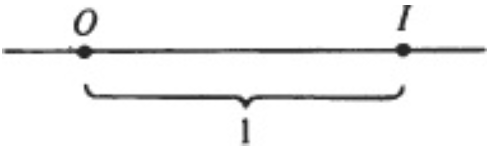
\includegraphics[width=0.3\textwidth]{pinter/assets/ch30-a-1.png}\par}

the interval $OI$ coincides with the unit interval on the $x$ axis. Let $\D$ be the set of real numbers such that $a\in\D$ if and only if the point $(a,0)$ is constructible from $\{O,I\}$. Prove the following
\begin{enumerate}
    \item If $a,b\in\D$, then $a+b\in\D$ and $a-b\in\D$.
    \item If $a,b\in\D$, then $ab\in\D$. (Hint: Use similar triangles. See the accompanying figure).
    
    {\centering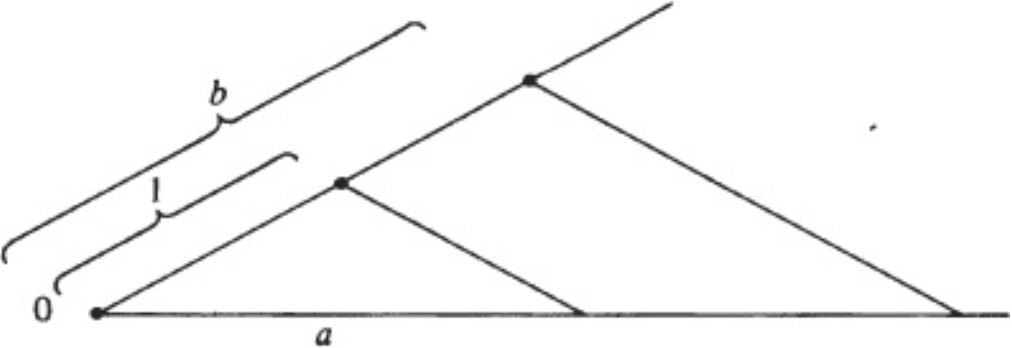
\includegraphics[width=0.5\textwidth]{pinter/assets/ch30-a-2.png}\par}
    \item If $a,b\in\D$, then $a/b\in\D$. (Use the same figure as in part 2).
    \item If $a>0$ and $a\in\D$, then $\sqrt{a}\in\D$. (Hint: In the accompanying figure, $AB$ is the diameter of a circle. Use an elementary property of chords of a circle to show that $x=\sqrt{a}$).
    
    {\centering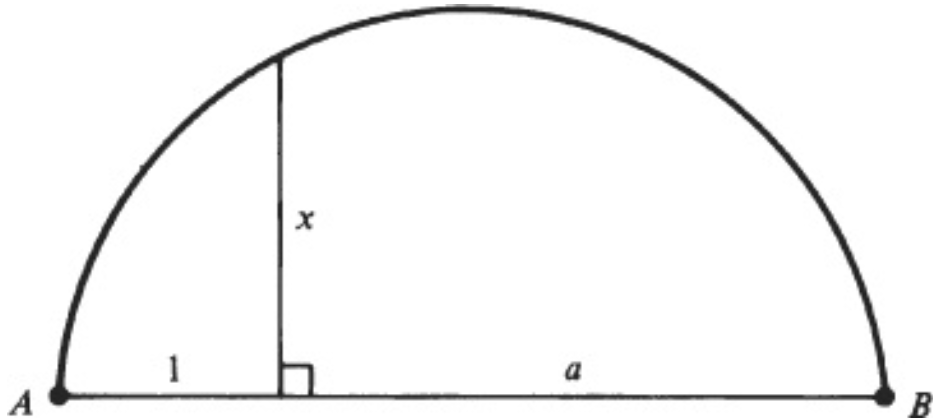
\includegraphics[width=0.5\textwidth]{pinter/assets/ch30-a-3.png}\par}

    It follows from parts 1 to 4 that $\D$ is a field, closed with respect to taking square roots of positive numbers. $\D$ is called the field of constructible numbers.
    \item $\Q\subset\D$.
    \item If $a$ is a real root of any quadratic polynomial with coefficients in $\D$, then $a\in\D$. (Hint: Complete the square and use part 4).
\end{enumerate}
\end{exercise}
\begin{proof}
 \begin{enumerate}
     \item Construct a circle around $A$ with radius $OB$. Without loss of generality, suppose $\lvert a\rvert>\lvert b\rvert$. If both $a$ and $b$ are positive, then take the furthest (from $O$) intersection of the circle with the $x$-axis. If $a$ is positive and $b$ is negative then take the closest intersection. Finally, if $a$ and $b$ are both negative, then take the furthermost point of the intersection. This gives us $a+b$. We can derive $a-b$ by using the same strategy but exchanging furthest for closest.
     \item
     \item
     \item 
     \item We have that $1\in\D$, since $a+b\in\D$, then all naturals are in $\D$. Furthermore, since all $a-b\in\D$ all integers are in $\D$. We can take this further by noticing that all quotients are in $\D$. Since $\Q$ are the quotients of all integers, then $\Q\in\D$. 
     \item
 \end{enumerate}
\end{proof}

\begin{exercise}{B Constructible points and constructible numbers}
Prove each of the following
\begin{enumerate}
    \item Let $\AAA$ be any set of points in the plane; $(a,b)$ is constructible from $\AAA$ if and only if $(a,0)$ and $(0,b)$ are constructible from  $\AAA$.
    \item If a point $P$ is constructible from $\{O,I\}$ [that is, from $(0,0)$ and $(1,0)$], then $P$ is constructible from $\Q\times\Q$.
    \item Every point in $\Q\times\Q$ is constructible from $\{O,I\}$. (Use ex.A.5. and the definition of $\D$).
    \item If a point $P$ is constructible from $\Q\times\Q$, it is constructible from $\{O,I\}$.

    By combining parts 2 and 4, we get the following important fact: Any point $P$ is constructible from $\Q\times\Q$ if and only if $P$ is constructible from $\{O,I\}$. Thus, we may define a point to be constructible if and only if it is constructible from $\{O,I\}$.
     \item A point $P$ is constructible if and only if both its coordinates are constructible numbers.
\end{enumerate}
\end{exercise}
\begin{proof}
 \begin{enumerate}
     \item 
     \item
     \item
     \item 
     \item
 \end{enumerate}
\end{proof}

\begin{exercise}{C Constructible angles}
An angle $\alpha$ is called constructible if and only if there exist constructible points $A,B$ and $C$ such that $\angle ABC=\alpha$. Prove the following:
\begin{enumerate}
    \item The angle $\alpha$ is constructible if and only if $\sin\alpha$ and $\cos\alpha$ are constructible numbers.
    \item $\cos\alpha\in\D$ if and only if $\sin\alpha\in\D$.
    \item If $\cos\alpha,\cos\beta\in\D$, then $\cos(\alpha+\beta),\cos(\alpha-\beta)\in\D$.
     \item $\cos(2\alpha)\in\D$ if and only if $\cos\alpha\in\D$.
     \item If $\alpha$ and $\beta$ are constructible angles, so are $\alpha+\beta,\alpha-\beta,(1/2)\alpha$ and $n\alpha$ for any positive integer $n$.
     \item The following angles are constructible: 30\degree, 75\degree, 22(1/2)\degree.
     \item The following angles are not constructible: 20\degree, 40\degree, 140\degree. (Hint: Use the proof of Theorem 3).
\end{enumerate}
\end{exercise}
\begin{proof}
 \begin{enumerate}
     \item 
    \item
    \item 
     \item
     \item
     \item 
     \item
 \end{enumerate}
\end{proof}

\begin{exercise}{D Constructible polygons}
A polygon is called constructible if and only if its vertices are constructible points. Prove the following:
\begin{enumerate}
    \item The regular $n$-gon is constructible if and only if the angle $2\pi/n$ is constructible. 
    \item The regular hexagon is constructible.
    \item The regular polygon of nine sides is not constructible.
\end{enumerate}
\end{exercise}
\begin{proof}
 \begin{enumerate}
     \item 
     \item
     \item
 \end{enumerate}
\end{proof}

\begin{exercise}{G Further properties of constructible numbers and figures}
Prove each of the following
\begin{enumerate}
    \item If the number $a$ is a root of an irreducible polynomial $p(x)\in\Q[x]$ whose degree is not a power of 2, then $a$ is not a constructible number.  
    \item Any constructible number can be obtained from rational numbers by repeated addition subtraction, multiplication, division, and taking square roots of positive numbers.
    \item $\D$ is the smallest field extension of $\Q$ closed with respect to square roots of positive numbers (that is, any field extension of $\Q$ closed with respect to square roots contains $\D$). (Use part 2 and exercise A).
    \item All the roots of the polynomial $x^4-3x^2+1$ are constructible numbers.

    A line is called constructible if it passes through two constructible points. A circle is called constructible if its center and radius are constructible.
    \item The line $ax+by+c=0$ is constructible if $a,b,c\in\D$.
    \item The circle $x^2+y^2+ax+by+c=0$ is constructible if $a,b,c\in\D$.
\end{enumerate}
\end{exercise}
\begin{proof}
 \begin{enumerate}
     \item 
     \item 
    \item
    \item 
    \item Suppose $a,b,c\in\D$. We have that $y=-(a/b)x-(c/b)$.
    \item
 \end{enumerate}
\end{proof}
\section*{Chapter 31. Galois Theory: Preamble}
\addcontentsline{toc}{section}{Chapter 31. Galois Theory: Preamble}


\begin{exercise}{A Examples of root fields over $\Q$}
\begin{enumerate}
    \item Show that $\Q(\sqrt{3},i)$ is the root field of $(x^2-2x-2)(x^2+1)$ over $\Q$.

    Comparing part 1 with the example, we note that different polynomials may have the same root field. This is true even if the polynomials are irreducible.
    \item Prove that $x^2-3$ and $x^2-2x-2$ are both irreducible over $\Q$. Then find their root fields over $\Q$ and show they are the same.
    \item Find the root field of $x^4-2$, first over $\Q$ then over $\R$.
    \item Explain: $\Q(i,\sqrt{2})$ is the root field of $x^4-2x^2+9$ over $\Q$, and is the root field of $x^2-2\sqrt{2}x+3$ over $\Q(\sqrt{2})$.
\end{enumerate}
\end{exercise}
\begin{proof}
 \begin{enumerate}
     \item This polynomial has as roots $i, -i, 1+\sqrt{3}, 1-\sqrt{3}$, all of which belong to $\Q(\sqrt{3}, i)$.
     \item The irreducibility of $x^2-3$ and $x^2-2x-2$ follows from Eisenstein's criterion using $p=3$ and $p=2$.

     We have that $x^2-3$ has as roots $\pm\sqrt{3}$, both of which are in $\Q(\sqrt{3})$, and $x^2-2x-2$ has roots $1\pm\sqrt{3}$, both of which belong to $\Q(\sqrt{3})$. Then the root fields of both polynomials are the same.
     \item In $\Q$, $x^4-2$ cannot be factorised further, so that its root field is $\Q(\sqrt[4]{2},i)$, whereas in $\R$, $x^4-2$ can be factorised into $x^4-2=(x^2-2)(x^2+2)=(x-\sqrt{2})(x+\sqrt{2})(x^2+2)$, so that its root field over $\R$ is $\R(i)=\C$, since the root of $x^2+2$ is $\sqrt{2}i$.
     \item Well, $x^4-2x^2+9$ over $\Q(\sqrt{2})$ can be factorized into $(x^2-2\sqrt{2}x+3)(x^2+2\sqrt{2}x+3)$. In this case, $x^2-2\sqrt{2}x+3$ has as roots $\sqrt{2}\pm i$ so that its root field is $\Q(\sqrt{2}, i)$ and $x^2+2\sqrt{2}x+3$ has as roots $-\sqrt{2}\pm i$ so that its root field is $\Q(\sqrt{2},i)$, so that only $(x^2-2\sqrt{2}x+3)$ or $(x^2+2\sqrt{2}x+3)$ defines the root field of the non-factored polynomial. 

     On the other hand, $x^4-2x^2+9$ cannot be factored over $\Q$, so that its roots are derived directly in there (the roots are the same as above) and its root field is $\Q(\sqrt{2},i)$.
 \end{enumerate}
\end{proof}

\begin{exercise}{B Examples of root fields over $\Z_p$}
\begin{enumerate}
    \item Show that, in any extension of $\Z_3$ which contains a root $u$ of $a(x)=x^3+2x+1\in\Z_3[x]$, it happens that $u+1$ and $u+2$ are the remaining two roots of $a(x)$. Use this fact to find the root field of $x^3+2x+1$ over $\Z_3$. List the elements of the root field.
\end{enumerate}
\end{exercise}
\begin{proof}
 \begin{enumerate}
     \item We have
     \begin{align*}
         (u+1)^3+2(u+1)+1 =& (u+1)(u^2+2u+1)+2u+2+1\\
         =& u^3+u^2+u+2u^2+2u+2+2u+2\\
         =& u^3+2u+1=0.
     \end{align*}
     Moreover,
     \begin{align*}
         (u+2)^2+2(u+2)+1 =& (u+2)(u^2+4u+4)+2u+4+1\\
         =& u^3+u^2+u+2u^2+2u+2+2u+2\\
         =& u^3+2u+1=0.
     \end{align*}
    So that the other roots of $x^3+2x+1$ are $u+1$ and $u+2$ as conjectured. The field $\Z_3(c)$ is isomorphic to $\quot{\Z_3[x]}{\langle x^3+2x+1\rangle}$, which are all the polynomials of degree less than 3 with coefficients in $\Z_3$. There are $3^3$ of these polynomials.
 \end{enumerate}
\end{proof}

\begin{exercise}{C Short questions relating to root field}
Prove each of the following
\begin{enumerate}
    \item Every extension of degree 2 is a root field.
    \item If $F\subseteq I\subseteq K$ and $K$ is a root field of $a(x)$ over $F$, then $K$ is a root field of $a(x)$ over $I$.
    \item The root field over $\R$ of any polynomial in $\R[x]$ is $\R$ or $\C$.
    \item If $c$ is a complex root of a cubic $a(x)\in\Q[x]$, then $\Q(c)$ is the root field of $a(x)$ over $\Q$. \textcolor{blue}{According to some online errata, this is false and one is encouraged to find a counterexample.}
    \item If $p(x)=x^4+ax^2+b$ is irreducible in $F[x]$, then $\quot{F[x]}{\langle p(x)\rangle}$ is the root field of $p(x)$ over $F$.
    \item If $K=F(a)$ and $K$ is the root field of some polynomial over $F$, then $K$ is the root field of the minimum polynomial of $a$ over $F$.
    \item Every root field over $F$ is the root field of some irreducible polynomial over $F$. [Hint: Use part 6 and Theorem 2].
    \item Suppose $[K:F]=n$, where $K$ is a root field over $F$. Then $K$ is the root field over $F$ of every irreducible polynomial of degree $n$ in $F[x]$ having a root in $K$. 
    \item If $a(x)$ is a polynomial of degree $n$ in $F[x]$, and $K$ is the root field of $a(x)$ over $F$, then $[K:F]$ divides $n!$.
\end{enumerate}
\end{exercise}
\begin{proof}
 \begin{enumerate}
     \item Suppose $K$ is an extension of $F$, with $[K:F]=2$. We can write $K=F(a)$ for a root $a$ of a polynomial $p(x)=x^2+bx+c$ of degree 2 in $F[x]$. But the roots of $p(x)$ are $b/2$ and $\pm\sqrt{b^2-4c}/2$. Since $[K=F(a):F]=2$ then it must be the case that $a=\sqrt{b^2-4c}/2$ or $a=-\sqrt{b^2-4c}/2$, but since $K=F(a)$ is a field, then we the negative of $a$ must also be in $K$ and so $K$ is the root field of $p(x)$.
    \item If $K$ is a root field of $a(x)$ over $F$, then $a(x)$ has coefficients in $F$, and $K$ is the smallest field containing all the roots of $a(x)$. Certainly all the coefficients of $a(x)$ are also in $I$, and furthermore, there is no smaller field containing the roots of $a(x)$, as otherwise this field would be the root field of $a(x)$ over $F$ as well.
    \item By the Fundamental Theorem of Algebra, we know that any univariate polynomial of degree greater than 0 has at least one complex root. If the polynomial has no complex roots, then $\R$ is the root field. If the polynomial has a complex root, then $\C=\R(i)$ is the root field, given that $\C$ contains the roots of all polynomials in $\R[x]$.
    \item Consider the polynomial $x^3+4x^2+6x-24$. The roots of this polynomial are two complex numbers of the form $a\pm ib$, where both $a$ and $b$ are irrational and a real number $c$ which is also irrational. Since the 
    \item Consider the polynomial $x^3+2$. This polynomial has as roots $-\sqrt[3]{2}$ and $1/2^{2/3}\pm i\sqrt{3}/2^{2/3}$. We cannot produce the real root as field operations on any of the complex roots, giving as the desired counterexample.
    \item If $K$ is the root field of some polynomial over $F$, then it is the smallest field that contains all the roots of such polynomial. We can identify $F(a)\cong\quot{F[x]}{\langle p(x)\rangle}$, where $p(x)$ is the minimal polynomial of $a$ over $F$. But we know that the polynomial of which $K$ is the root field of, must be a product of $p(x)$, and because the roots of such polynomial are only the roots of $p(x)$, then $K$ must the root field of $p(x)$ too.
    \item From part 6, we know that a root field $K=F(a)$ is the root field of the minimum polynomial of $a$ over $F$. For an arbitrary root field $K=F(a_1,\dots,a_n)$, we can represent $K$ as $F(a)$ by Theorem 2. Hence, $K$ is the minimum polynomial of $a$ over $F$, but minimum polynomials are also irreducible, so that any root field $K$ over $F$ is the root field of an irreducible polynomial.
    \item All the hypotheses of Theorem 7 are met so this is a Corollary to that Theorem.
    \item We start by stating some known facts. We know that a polynomial of degree $n$ has at most $n$ distinct roots, and that $[K:F]$ is the degree of $K$ over $F$. Furthermore, we can represent $K$ as a simple extension $F(c)$. We have that $[F(c):F]$ equals the minimum polynomial of $c$ over $F$. But we know that this is at most $a(x)$, as otherwise $K$ would not be a root field of $a(x)$, so that $[F(c):F]$ is at most $n$. Finally, since $n!$ contains the product of all naturals less than or equal to $n$, then it must be the case that $[K=F(c):F]$ divides $n!$.
 \end{enumerate}
\end{proof}

\begin{exercise}{D Reducing iterated extensions to simple extensions}
\begin{enumerate}
    \item Find $c$ such that $\Q(\sqrt{2},\sqrt{-3})=\Q(c)$. Do the same for $\Q(\sqrt{2},\sqrt[3]{2})$.
\end{enumerate}
\end{exercise}
\begin{proof}
 \begin{enumerate}
     \item We will use the result of Theorem 2 to solve this exercise. 
     
     First we consider $\Q(\sqrt{2},\sqrt{-3})$. We have that the minimum polynomial of $\sqrt{2}$ over $\Q$ is $x^2-2$ which has $\pm\sqrt{2}$ as roots. On the other hand, the minimum polynomial of $\sqrt{-3}$ is $x^2+3$, with roots $\pm\sqrt{-3}$. We then define $t=1\neq (-\sqrt{2}-\sqrt{2})/(-\sqrt{-3}-\sqrt{-3})$, so that $c=\sqrt{2}+\sqrt{-3}$ and $\Q(\sqrt{2},\sqrt{-3})=\Q(\sqrt{2}+\sqrt{-3})$.

     Now we consider $\Q(\sqrt{2},\sqrt[3]{2})$. The minimum polynomial of $\sqrt{2}$ is as above. On the other hand, the minimum polynomial of $\sqrt[3]{2}$ is $x^3-2$ which has $\sqrt[3]{2}$ and $-(1/2^{2/3})\pm i(\sqrt[3]{2}/2^{2/3})$ as roots. Defining $t=1\neq (a_i-\sqrt{2})/(\sqrt[3]{2}-b_j)$ for all $i$ and $j$, we get that $\Q(\sqrt{2},\sqrt[3]{2})=\Q(\sqrt{2}+\sqrt[3]{2})$, as required.
 \end{enumerate}
\end{proof}

\begin{exercise}{H An isomorphism extension Theorem (Proof of Theorem 3)}
Let $F_1,F_2,h,p(x),a,b$ and $\bar{h}$ be as in the statement of Theorem 3. To prove that $\bar{h}$ is an isomorphism, it must first be shown that it is properly defined: that is, if $c(a)=d(a)$ in $F_1(a)$, then $\bar{h}(c(a))=\bar{h}(d(a))$.
\begin{enumerate}
    \item If $c(a)=d(a)$, prove that $c(x)-d(x)$ is a multiple of $p(x)$. Deduce from this that $hc(x)-hd(x)$ is a multiple of $hp(x)$.
    \item Use part 1 to prove that $\bar{h}(c(a))=\bar{h}(d(a))$.
    \item Reversing the steps of the preceding argument, show that $\bar{h}$ is injective.
    \item Show that $\bar{h}$ is surjective.
    \item Show that $\bar{h}$ is a homomorphism.
\end{enumerate}
\end{exercise}
\begin{proof}
 \begin{enumerate}
     \item If $c(a)=d(a)$, then $c(a)-d(a)=0$. Since $p(x)$ is irreducible, and $a$ is a root of $p(x)$, then $p(x)$ is the minimum polynomial of $a$ in $F_1$. Hence, any polynomial whose root is $a$ is a multiple of $p(x)$ and $c(x)-d(x)$ is a multiple of $p(x)$.

     We have $c(x)-d(x)=p(x)q(x)$ for some polynomial $q(x)$. Then, $h(c(x)-d(x))=h(c(x))-h(d(x))=h(p(x)q(x))=h(p(x))h(q(x))$, as required.
     \item Evaluating $h(c(x))-h(d(x))=h(p(x))h(q(x))$ at $a$ gives us $\bar{h}(c(a))-\bar{h}(d(a))=\bar{h}(p(a))\bar{h}(q(a))=0$ so that $\bar{h}(c(a))=\bar{h}(d(a))$, as required.
     \item Suppose $\bar{h}(c(a))=\bar{h}(d(a))$. Then $\bar{h}(c(a))-\bar{h}(d(a))=0$ and $h(c(x))-h(d(x))$ is a multiple of $h(p(x))$ since it has $\bar{h}(a)$ as root. Hence, $c(x)-d(x)$ is a multiple of $p(x)$, and $c(a)-d(a)=p(a)q(a)=0$ so that $c(a)=d(a)$, as required.
     \item Since all elements of $F_2(b)$ are of the form $d_0+d_1b+\dots+d_nb^n$, and $h$ is an isomorphism, then there is an element of $F_1(a)$ corresponding to $h^{-1}(d_0)+\dots+h^{-1}(d_n)a^n$, as required.
     \item Since every element of $F_1(a)$ is of the form $c_0+c_1a+\dots+c_na^n$ and $\bar{h}$ maps this element to $h(c_0)+h(c_1)b+\dots+h(c_n)b^n$, then the homomorphism properties follow by the usual addition and multiplication properties of polynomials and the fact that $h$ is itself an isomorphism.
 \end{enumerate}
\end{proof}

\begin{exercise}{I Uniqueness of the root field}
Let $h:F_1\rightarrow F_2$ be an isomorphism. If $a(x)\in F_1[x]$, let $K_1$ be the root field of $a(x)$ over $F_1$, and $K_2$ the root field of $ha(x)$ over $F_2$.
\begin{enumerate}
    \item Prove: if $p(x)$ is an irreducible factor of $a(x),u\in K_1$ is a root of $p(x)$, and $\nu\in K_2$ is a root of $hp(x)$, then $F_1(u)\cong F_2(\nu)$.
    \item $F_1(u)=K_1$ if and only if $F_2(\nu)=K_2$.
    \item Use parts 1 and 2 to form and inductive proof that $K_1\cong K_2$.
    \item Draw the following conclusion: the root field of a polynomial $a(x)$ over a field $F$ is unique up to isomorphism.
\end{enumerate}
\end{exercise}
\begin{proof}
 \begin{enumerate}
     \item Since $p(x)$ is irreducible in $F_1[x]$, $u$ is a root of $p(x)$ and $v$ is a root of $hp(x)$, by Theorem 3, $h$ can be extended to an isomorphism between $F_1(u)$ and $F_2(v)$.
     \item We have that $F_1(u)=K_1$ if and only if $F_1(u)$ has all the roots of $a(x)$, but by exercise 1, there is an extension of $h$ such that $F_1(u)\cong F_2(v)$, but this is true if and only if $F_2(v)$ contains all the roots of $ha(x)$, that is, if $F_2(v)=K_2$, as required.
     \item Consider the following factorization of $a(x)=a_1(x)\dots a_n(x)$, where each $a_i(x)$ is irreducible. Now for the base case, if $u_1$ is a root of $a_1(x)$ and $v_1$ is a root of $ha_1(x)$, we can use exercise 1 to conclude that $F_1(u_1)\cong F_2(v_2)$. Now we can reason inductively by using $F_1(u_1)$ and $F_2(v_2)$ as the starting fields, and the extension of $h$ as the initial isomorphism. When we do this for all $a_i(x)$, we have that $K_1\cong K_2$, as required.
     \item This is exactly the content of the previous exercise. That is, any two extensions that are root fields of $a(x)$ have to be isomorphic.
 \end{enumerate}
\end{proof}

\begin{exercise}{K Normal extensions}
If $K$ is the root field of some polynomial $a(x)$ over $F, K$ is also called a normal extension of $F$. There are other possible ways of defining normal extensions, which are equivalent to the above. We consider the two most common ones here: they are precisely the properties expressed in Theorems 7 and 6. Let $K$ be a finite extension of $F$.
\begin{enumerate}
    \item Suppose that for every irreducible polynomial $p(x)$ in $F[x]$, if $p(x)$ has one root in $K$, then $p(x)$ must have all its roots in $K$. Prove that $K$ is a normal extension of $F$.
    \item Suppose that, if $h$ is any isomorphism with domain $K$ which fixes $F$, then $h(K)\subseteq K$. Prove that $K$ is a normal extension of $F$.
\end{enumerate}
\end{exercise}
\begin{proof}
 \begin{enumerate}
     \item Since $K$ is a finite extension of $F$, then we can write $K$ as a simple extension $F(c)$ for some $c$. Then if we take $p(x)$ to be the minimum polynomial of $c$ in $F$, and recalling that minimum polynomials are irreducible, we have that $F(c)$ is the root field of $p(x)$. That is, a normal extension of $F$.
     \item Because $K$ is a finite extension of $F$ we can write $K=F(c)$ for some $c$. Let $p(x)$ the minimum polynomial of $c$, and let $L$ be the root field of $p(x)$, we have that $F\subseteq K\subseteq L$. We want to prove that $K=L$. Let $a$ be a root in $L\setminus K$. Now consider the extension of $h$ to $\bar{h}:K\rightarrow L$, that sends $a$ to $c$. But because the homomorphism between two fields is injective, and we have that $h(K)\subseteq K$, then the homomorphism is surjective so that $K=L$. That is, $K$ is a normal extension of $F$.
 \end{enumerate}
\end{proof}
\subsection*{Chapter 32. Galois Theory: the Heart of the Matter}
\addcontentsline{toc}{subsection}{Chapter 32. Galois Theory: the Heart of the Matter}


\begin{exercise}{A Computing a Galois group}
\begin{enumerate}
    \item Show that $\Q(i,\sqrt{2})$ is the root field of $(x^2+1)(x^2-2)$ over $\Q$.
    \item Find the degree of $\Q(i,\sqrt{2})$ over $\Q$.
    \item List the elements of $Gal(\Q(i,\sqrt{2}):\Q)$ and exhibit its table.
    \item Write the inclusion diagram for the subgroups of $Gal(\Q(i,\sqrt{2}):\Q)$, and the inclusion diagram for the fields intermediate between $\Q$ and $\Q(i,\sqrt{2})$. Indicate the Galois correspondence.
\end{enumerate}
\end{exercise}
\begin{proof}
 \begin{enumerate}
     \item The roots of $x^2+1$ are $\pm i$ and the roots of $x^2-2$ are $\pm\sqrt{2}$, so that $\Q(i,\sqrt{2})$ is the root field of $(x^2+1)(x^2-2)$.
     \item We know that $[Q(i,\sqrt{2}:\Q]=[Q(i,\sqrt{2}):\Q(i)][\Q(i):\Q]=2\cdot 2=4$.
     \item Following a similar approach to the example in the chapter, we have that $e$ is the transformation that leaves the roots invariant, $\alpha$ transforms $\sqrt{2}$ into $-\sqrt{2}$, $\beta$ transforms $i$ into $-i$ and $\gamma$ transforms both $\sqrt{2}$ and $i$ into their negative counterparts. The multiplication table is the same as $Gal(\Q(\sqrt{2},\sqrt{3}):\Q)$.
     \item The Galois correspondence is the same as the correspondence between $Gal(\Q(\sqrt{2},\sqrt{3}):\Q)$ and the intermediate fields of $\Q(\sqrt{2},\sqrt{3})$. The main difference is that $\Q(\sqrt{6})$ is replaced by $\Q(i\sqrt{2})$, which is the fixfield of the subgroup $\{e,\gamma\}\in Gal(\Q(\sqrt{2},\sqrt{3}):\Q)$.
 \end{enumerate}
\end{proof}

\begin{exercise}{B Computing a Galois group of eight elements}
\begin{enumerate}
    \item Show that $\Q(\sqrt{2},\sqrt{3},\sqrt{5})$ is the root field of $(x^2-2)(x^2-3)(x^2-5)$ over $\Q$.
    \item Show that the degree of $\Q(\sqrt{2},\sqrt{3},\sqrt{5})$ over $\Q$ is 8.
    \item List the 8 elements of $\mathbf{G}=Gal(\Q(\sqrt{2},\sqrt{3},\sqrt{5}):Q)$ and write its table.
    \item List the subgroups of $\mathbf{G}$. (By Lagrange's Theorem, any proper subgroup of $\mathbf{G}$ has either two or four elements).
     \item For each subgroup of $\mathbf{G}$ find its fixfield.
     \item Indicate the Galois correspondence by means of a diagram like the one on page 329.
\end{enumerate}
\end{exercise}
\begin{proof}
 \begin{enumerate}
     \item We have that $\pm\sqrt{2}$ are the roots of $x^2-2$, $\pm\sqrt{3}$ the roots of $x^2-3$, and $\pm\sqrt{5}$ the roots of $x^2-5$, so that $\Q(\sqrt{2},\sqrt{3},\sqrt{5})$ is the root field of $(x^2-2)(x^2-3)(x^2-5)$ over $\Q$.
     \item We know that 
     \begin{align*}
         [\Q(\sqrt{2}&,\sqrt{3},\sqrt{5}):\Q]\\
         =& [\Q(\sqrt{2},\sqrt{3},\sqrt{5}):\Q(\sqrt{2},\sqrt{3})][\Q(\sqrt{2},\sqrt{3}):\Q]\\
         =& [\Q(\sqrt{2},\sqrt{3},\sqrt{5}):\Q(\sqrt{2},\sqrt{3})][\Q(\sqrt{2},\sqrt{3}):\Q(\sqrt{2})][\Q(\sqrt{2}):\Q]\\
         =& 2\cdot 2\cdot 2=8,
     \end{align*}
     as required.
     \item The 8 elements of $\bG$ are the automorphisms that change the roots $\sqrt{2},\sqrt{3}$ and $\sqrt{5}$ for its negative counterparts. Since there are 3 square roots, there are $2^3$ automorphisms including the automorphism that changes no square roots (the identity) and the one that changes all. 
     \item Taking the example on the book as reference, we can see that each element of $\bG$ with the identity element forms a subgroup of $\bG$, furthermore, that gives us 6 subgroups (and 8 if we count the trivial subgroups). Furthermore, for each pair in $\{2,3,5\}$, we can take the subgroup that includes the automorphism that send each square root to its negative and that takes their product to their negative. For example, the automorphisms that: take $\sqrt{2}$ to its negative, take $\sqrt{3}$ to its negative, and take $\sqrt{6}$ to its negative plus the identity form a subgroup of $\bG$. Since there are 3 elements in the set above, there are $C(3,2)=3$ such subgroups. Giving us a total of 11 subgroups of $\bG$.
     \item For each subgroup of order 2, their fixfield is simply the field extension of the element which is taken to its negative: $\sqrt{2}, \sqrt{3}, \sqrt{5},\sqrt{6}, \sqrt{10},\dots$. For the subgroups of order 4, the  fixfields are the combinations of those roots that are changed: $\Q(\sqrt{2},\sqrt{3}), \Q(\sqrt{2},\sqrt{5}),\dots$. Notice that, for example $\Q(\sqrt{6})\subseteq\Q(\sqrt{2},\sqrt{3})$.
     \item The correspondence follows directly from the previous exercise. The figure would have 4 hierarchies instead of 3 as in the book example.
 \end{enumerate}
\end{proof}

\begin{exercise}{H The group of automorphisms of $\C$}
\begin{enumerate}
    \item Prove: the only automorphism of $\Q$ is the identity function. [Hint: if $h$ is an automorphism, $h(1)=1$; hence $h(2)=2$, and so on].
    \item Prove: any automorphism of $\R$ sends squares of numbers to squares of numbers, hence positive numbers to positive numbers.
    \item Using part 2, prove that if $h$ is any automorphism of $\R$, $a<b$ implies $h(a)<h(b)$.
    \item Use parts 1 and 3 to prove that the only automorphism of $\R$ is the identity function.
     \item List the elements of $Gal(\C:\R)$.
     \item Prove that the identity function and the function $a+bi\rightarrow a-bi$ are the only autmorphisms of $\C$ which fix $\R$.
\end{enumerate}
\end{exercise}
\begin{proof}
 \begin{enumerate}
     \item Let $h$ be an automorphism of $\Q$. We will first prove by induction that for all $n\in\N$, $h(n)=n$. For the base case, notice that $h(1)=1$ by the properties of homomorphisms. Now suppose the statement holds for $n$. We then have $h(n+1)=h(n)+h(1)=n+1$, as required. By the properties of ring homomorphisms, we have that $h(-n)=-h(n)=-n$, so that $h$ maps every integer to itself. Finally, by the properties of ring homomorphisms, $h(n^{-1})=h(n)^{-1}=n^{-1}$. Notice that any rational can be represented as $m/n$ for integers $m$ and $n$. So that $h(m/n)=h(m)h(n)^{-1}=m/n$. That is, $h$ is the identity.
     \item Let $h$ be an automorphism of $\R$, and let $a\in\R$. We have $h(a^2)=h(aa)=h(a)h(a)=h(a)^2$, as required.
     \item Because $b>a$, there exists an element $x\in\R$ so that $b-a=x^2$. From 2, we know that $h(x^2)=h(x)^2$ so that $h(b-a)=h(b)-h(a)$ is positive and hence $h(b)>h(a)$.
     \item Suppose, for the sake of contradiction that there exists a real $x$ with $h(x)\neq x$. Suppose without loss of generality that $x>h(x)$. Then there exists a rational, $a$ so that $h(x)<a<x$. But notice that by 3, if $x>a$, then $h(x)>h(a)$, and by 1, $h(a)=a$, so that $h(x)<a<x$ is a contradiction.
     \item By Theorem 1, the degree of $Gal(\C:\R)=2$. Then, we know that the automorphisms of $\C$ which fix $\R$ are simply those automorphisms that send $a+bi$ to itself or that send it to $a-bi$.
     \item This is the same as the question above.
 \end{enumerate}
\end{proof}

\begin{exercise}{I Further questions relating to Galois groups}
Throughout this set of questions, let $K$ be a root field over $F$, let $\mathbf{G}=Gal(K:F)$, and let $I$ be any intermediate field. Prove the following:
\begin{enumerate}
    \item $I^\ast=Gal(K:I)$ is a subgroup of $\mathbf{G}$.
    \item If $H$ is a subgroup of $\mathbf{G}$ and $H^\circ=\{a\in K: \pi(a)=a\text{ for every }\pi\in H\}$, then $H^\circ$ is a subfield of $K$, and $F\subseteq H^\circ$.
    \item Let $H$ be the fixer of $I$, and $I'$ the fixfield of $H$. Then $I\subseteq I'$. Let $I$ be the fixfield of $H$, and $I^\ast$ the fixer of $I$. Then $H\subseteq I^\ast$.
    \item Let $I$ be a normal extension of $F$ (that is, a root field of some polynomial over $F$). If $\mathbf{G}$ is abelian, then $Gal(K:I)$ and $Gal(I:F)$ are abelian. (Hint: Use Theorem 4).
     \item Let $I$ be a normal extension of $F$. If $\mathbf{G}$ is a cyclic group, then $Gal(K:I)$ and $Gal(I:F)$ are cyclic groups.
     \item If $\mathbf{G}$ is a cyclic group, there exists exactly one intermediate field $I$ of degree $k$, for each integer $k$ dividing $[K:F]$.
\end{enumerate}
\end{exercise}
\begin{proof}
 \begin{enumerate}
     \item Let $g,h\in I^\ast$. We know that $I^\ast$ is closed under composition because if $g$ and $h$ fix $I$, then certainly $g\circ h$ and $h\circ g$ too. Furthermore, since $g$ moves only elements of $K$ that are not in $I$, then $g^{-1}$ moves only those elements that are originally moved, in other words, $g^{-1}$ fixes $I$, so that it is in $I^\ast$. Hence, $I^\ast$ is a subgroup of $\bG$.
     \item Let $a,b\in H^\circ$. For all $\pi\in H$, we have that $\pi(a-b)=\pi(a)-\pi(b)=a-b$ so that $a-b$ is also fixed by the elements of $H$. Furthermore, $\pi(ab)=\pi(a)\pi(b)=ab$, so that $ab$ is also fixed by the elements of $H$. As a result, $H^\circ$ is a subfield of $K$.

     To prove that $F\subseteq H^\circ$, notice that because $\bG=Gal(K:F)$, then $F$ is fixed by any element of $\bG$ and hence by any subgroup of $\bG$, so that $F$ is contained in $H^\circ$.
     \item By definition, if $H$ is the fixer of $I$, all elements of $H$ fix $I$. On the other hand, $I'$ the fixfield of $H$, contains all the elements in $K$ that are not moved by all elements of $H$. Hence for $a\in I$, $a\in I'$ and $I\subseteq I'$.

     If $I$ is the fixfield of $H$, then all the elements in $I$ are not moved by all the elements of $H$. Likewise, if $I^\ast$ is the fixer of $I$, then all the elements of $I^\ast$ fix $I$, as a result, $H\subseteq I^\ast$.
     \item We know that $Gal(K:I)$ is abelian because from exercise 1, $Gal(K:I)\subseteq Gal(K:F)$ an any subgroup of an abelian group is abelian.

     To conclude that $Gal(I:F)$ is abelian, notice that from Theorem 4, $Gal(I:F)\cong\quot{Gal(K:F)}{Gal(K:I)}$. But from group theory, we know that the quotient of an abelian group is abelian, then $Gal(I:F)$ is abelian as desired.
     \item Since $Gal(K:I)$ is a subgroup of $Gal(K:F)$, and we know that the subgroup of a cyclic group is cyclic, then $Gal(K:I)$ is cyclic.

     Again, by Theorem 4, we have that $Gal(I:F)\cong\quot{Gal(K:F)}{Gal(K:I)}$. But the quotient of a cyclic group is cyclic, so that $Gal(I:F)$ is cyclic, as desired.
     \item First, we know that the intermediate fields between $K$ and $I$ are identified by the subgroups of $\bG$ by the Galois correspondence. Hence, we can write this question in its group-only form as: ``If $\bG$ is cyclic, there exists exactly one subgroup of order $k$ for each integer dividing the order of $\bG$''. But this is a result from group theory, so that the desired result is fulfilled.
 \end{enumerate}
\end{proof}

\begin{exercise}{J Normal extensions and normal subgroups}
Suppose $F\subseteq K$, where $K$ is a normal extension of $F$. (This means simply that $K$ is the root field of some polynomial in $F[x]$: see Chapter 31 exercise K). Let $I_1\subseteq I_2$ be intermediate fields.
\begin{enumerate}
    \item Deduce from Theorem 4 that, if $I_2$ is a normal extension of $I_1$, then $I^\ast_2$ is a normal subgroup of $I^\ast_1$.
    \item Prove the following for any intermediate field $I$: Let ${h\in Gal(K:F)},\, g\in I^\ast,\, a\in I$, and $b=h(a)$. Then $[h\circ g\circ h^{-1}](b)=b$. Conclude that $hI^\ast h^{-1}\subseteq h(I)^\ast$.
    \item Use part 2 to prove that $hI^\ast h^{-1}=h(I)^\ast$.

    Two intermediate fields $I_1$ and $I_2$ are called conjugate if and only if there is an automorphism [i.e., an element $i\in Gal(K:F)$] such that $i(I_1)=I_2$.
    \item Use part 3 to prove that $I_1$ and $I_2$ are conjugate if and only if $I^\ast_1$ and $I^\ast_2$ are conjugate subroups in the Galois group.
    \item Use part 4 to prove that for any intermediate fields $I_1$ and $I_2$: if and only if $I^\ast_2$ is a normal subgroup of $I^\ast_1$, then $I_2$ is a normal extension of $I_1$.

    Combining parts 1 and 5 we have: $I_2$ is a normal extension of $I_1$ if and only if $I^\ast_2$ is a normal subgroup of $I^\ast_1$. (Historically, this result is the origin of the word ``normal'' in the term ``normal subrgroup'').
\end{enumerate}
\end{exercise}
\begin{proof}
 \begin{enumerate}
     \item We have that $I_1^\ast=Gal(K:I_1)$ and $I_2^\ast=Gal(K:I_2)$. Furthermore, if $I_1\subseteq I_2\subseteq K$, and $I_2$ is a normal extension of $I_1$ and $K$ is a normal extension of $I_1$ because $F\subseteq I_1\subseteq K$ and $K$ is a normal extension of $F$. Then by Theorem 4, we would have that $Gal(I_2:I_1)=\quot{Gal(K:I_1)}{Gal(K:I_2)}=\quot{I_1^\ast}{I_2^\ast}$ and $I_2^\ast$ is a normal subgroup of $I_1^\ast$.
     \item By definition, $h^{-1}(b)=a$, but $a\in I$, and $g\in I^\ast$, so that $g(a)=a$. Finally, by definition $h(a)=b$. Putting all of these together, we have $[h\circ g\circ h^{-1}](b)=b$. 

     Since the chosen $a, b$ and $g$ were arbitrary, that means that any element of $hI^\ast h^{-1}$ fixes any element of $I$ mapped by $h$, mathematically, $hI^\ast h^{-1}\subseteq h(I)^\ast$.
     \item We already proved that $hI^\ast h^{-1}\subseteq h(I)^\ast$. We will now prove that $hI^\ast h^{-1}$ has the same number of elements as $h(I)^\ast$. Since $h$ is an automorphism, $h(I)^\ast$ must have the same number of elements as $I^\ast$. Likewise, $hI^\ast h^{-1}$ must have the same elements as $I^\ast$. Hence, $h(I)^\ast$ and $hI^\ast h^{-1}$ have the same number of elements and using part 2, they are equal.
     \item ($\Rightarrow$) Suppose $I_1$ and $I_2$ are conjugate. Then there exists $h\in Gal(K:F)$ such that $h(I_1)=I_2$, which implies $h(I_1)^\ast=I_2^\ast$. By 3, we have $I_2^\ast= h(I_1)^\ast= hI_1^\ast h^{-1}$, so that $I_1^\ast$ and $I_2^\ast$ are conjugate, as desired.

     ($\Leftarrow$) Suppose $I_1^\ast$ and $I_2^\ast$ are conjugate. Then there exists $h\in Gal(K:F)$ such that $hI_1^\ast h^{-1}=I_2^\ast$. By 3, $I_2^\ast= hI_1^\ast h^{-1}= h(I_1)^\ast$. But then $I_2=h(I_1)$. which means that $I_1$ and $I_2$ are conjugate fields, as required.
    \item ($\Rightarrow$) We will use the following Lemma: a field extension is normal if and only if it equals all its conjugates. We will only prove the converse, as this is the only result we need for the exercise. For the proof, suppose a field $F$ equals all its conjugates, and let $K$ be a root field containing $F$. Furthermore, assume $F\neq K$. Take an irreducible polynomial so that some but not all its roots are in $F$. However, by Theorem 7 of Chapter 31, $K$ must contain all the roots of $p(x)$, and there must be an automorphism that permutes the roots of said polynomial. But because $F$ is its only conjugate then, by definition, all automorphisms send $F$ to itself. Hence, $F$ must contain all the roots of that polynomial, as all the automorphisms that permute the roots always send $F$ to itself. 

    For the proof of the exercise, let $I_2^\ast$ be a normal subgroup of $I_1^\ast$. By the definition of normal subgroup, $I_2^\ast$ is conjugate to itself. By exercise 4, $I_2$ is conjugate to itself, and by the lemma above, $I_2$ is a normal extension. Finally, because $I_2^\ast\subseteq I_1^\ast$, then $I_2\subseteq I_2$ which implies $I_2$ is a normal extension of $I_1$.
    
    ($\Leftarrow$) This is the content of exercise 1.
 \end{enumerate}
\end{proof}
\subsection*{Chapter 33. Solving Equations by Radicals}
\addcontentsline{toc}{subsection}{Chapter 33. Solving Equations by Radicals}


\begin{exercise}{A Finding radical extensions}
\begin{enumerate}
    \item Find radical extensions of $\Q$ containing the following complex numbers:
    \begin{enumerate}
        \item $(\sqrt{5}-\sqrt[5]{2})/(\sqrt[4]{3}+\sqrt[3]{4})$.
        \item $\sqrt{(1-\sqrt[9]{2})/\sqrt[3]{1-\sqrt{5}}}$.
        \item $\sqrt[5]{(\sqrt{3}-2i)^3/(i-\sqrt{11}}$.
    \end{enumerate}
    \item Show that the following polynomials in $\Q[x]$ are not solvable by radicals:
    \begin{enumerate}
        \item $2x^5-5x^4+5$.
        \item $x^5-4x^2+2$.
        \item $x^5-4x^4+2x+2$.
    \end{enumerate}
    \item Show that $a(x)=x^5-10x^4+40x^3-80x^2+79x-30$ is solvable by radicals over $\Q$, and give its root field. [Hint: Compute $(x-2)^5-(x-2)$].
    \item Show that $ax^8+bx^6+cx^4+dx^2+e$ is solvable by radicals over any field. [Hint: Let $y=x^2$; use the fact that every fourth degree polynomial is solvable by radicals].
    \item Explain why parts 3 and 4 do not contradict the principal finding of this chapter: that polynomial equations of degree greater than or equal to 5 do not have general solution by radicals.
\end{enumerate}
\end{exercise}
\begin{proof}
 \begin{enumerate}
     \item 
     \item
     \begin{enumerate}
         \item By Eisenstein's criterion, the polynomial is not reducible. Furthermore, the polynomial has two local optima at $x=0$ and $x=2$, so that it has three real roots and two complex roots, all denoted as $r_i$. Hence, we have that, if we denote $K$ as the root field of the polynomial, $[K:\Q]=[K:\Q(r_1)][\Q(r_1):\Q]=[K:\Q(r_1)]\cdot 5$. Hence, 5 is a factor of $[K:\Q]$, so that there is a 5-cycle in $[K:\Q]$. Finally, since the polynomial has two complex roots, we have the transposition given by $a+bi\to a-bi$ in $Gal(K:\Q)$ which implies that $Gal(K:\Q)\cong S_5$ so that the polynomial is unsolvable.
         \item As above, by Eisenstein's criterion, the polynomial is irreducible. Furthermore, it has two local optima, giving us 3 real roots and 2 complex roots. The rest of the proof follows as above.
         \item Same technique as above, though this time the optimum have no closed form. Nevertheless, this has no impact on the proof technique. 
     \end{enumerate}
     \item We have that $a(x)=x^5-10x^4+40x^3-80x^2+79x-30= (x-2)(x-3)(x-1)(x^2-4x+5)$, so that it has 2, 3 and 1 as real roots, and $2\pm i$ as complex roots and hence is solvable.
     \item If we do the substitution $y=x^2$, we obtain the polynomial given by $p(y)=ay^4+by^3+cy^2+dy+e$. Since every polynomial of fourth degree is solvable, then we can obtain the roots of the above polynomial by radicals. For any root $r_i$ of $p(y)$, we can substitute $\sqrt{r_i}$ which is a root of the original polynomial. Hence, the original polynomial is solvable by radicals.
    \item Neither 3 or 4 contradict the unsolvability of the quintic because the unsolvability of the quintic talks about the solution by radicals of a general quintic. Both 3 and 4 are specific cases of polynomials.
 \end{enumerate}
\end{proof}

\begin{exercise}{B Solvable groups}
Let $G$ be a group. The symbol $H\triangleleft G$ is commonly used as an abbreviation of ``$H$ is a normal subgroup of $G$''. A normal series of $G$ is a finite sequence $H_0,H_1,\dots,H_n$ of subgroups of $G$ such that $\{e\}=H_0\triangleleft H_1\triangleleft\dots\triangleleft H_n=G$. Such a series is called a solvable series if each quotient group $\quot{H_{i+1}}{H_i}$ is abelian. $G$ is called a solvable group if it has a solvable series.
\begin{enumerate}
    \item Explain why every abelian subgroup is, trivially, a solvable group.
    \item Let $G$ be a solvable group. with a solvable series $H_0,\dots,H_n$. Let $K$ be a subgroup of $G$. Show that $J_0=K\cap H_0,\dots,J_n=K\cap H_n$ is a normal series of $K$.
    \item Use the remark immediately preceding Theorem 2 to prove that $J_0,\dots,J_n$ is a solvable series of $K$.
     \item Use parts 2 and 3 to prove: every subgroup of a solvable group is solvable.
     \item Verify that $\{e\}\subseteq\{e,\beta,\delta\}\subseteq S_3$ is a solvable series for $S_3$. Conclude that $S_3$, and all of its subgroups, are solvable.
     \item In $S_4$, let $A_4$ be the group of all the even permutations, and let $B=\{e,(12)(34),(13)(24),(14)(23)\}$. Show that $\{e\}\subseteq B\subseteq A_4\subseteq S_4$ is a solvable series for $S_4$. Conclude that $S_4$ and all its subgroups are solvable.
\end{enumerate}
\end{exercise}
\begin{proof}
 \begin{enumerate}
     \item We have the chain given by $\quot{G}{\{e\}}\cong G$ which is abelian, giving us our desired chain.
     \item
     \item 
     \item
     \item
     \item
 \end{enumerate}
\end{proof}

\newpage
\section{Topoi}
\section*{Chapter 3 Arrows instead of epsilon}

\begin{exercise}{3.1 Monic arrows}
In any category 
\begin{enumerate}
    \item $g\circ f$ is monic if both $f$ and $g$ are monic.
    \item If $g\circ f$ is monic, then so is $f$.
\end{enumerate}
\end{exercise}
\begin{proof}
 \begin{enumerate}
     \item Suppose both $f$ and $g$ are monic. Then for any morphisms $l, h$, both $f\circ l = f\circ h$ and $g\circ l= g\circ h$ imply $l=h$. We have $(g\circ f) \circ l = (g\circ f) \circ h\implies g\circ (f\circ l) = g\circ(f \circ h) \implies g \circ l = g\circ h\implies l=h$, so that $g\circ f$ is monic.
     \item Suppose $g\circ f$ is monic. Then for any morphisms $l, h$, we have that $(g\circ f)\circ l=(g\circ f)\circ h$ implies $l=h$. Suppose now $f\circ l=f\circ h$, apply $g$ on both sides of the equation to get $(g\circ f)\circ l=(g\circ f)\circ h$, which implies $l=h$, as required.
 \end{enumerate}
\end{proof}

\begin{exercise}{3.3 Iso arrows}
\begin{enumerate}
    \item Every identity arrow is iso.
    \item If $f$ is iso, so is $f^{-1}$.
    \item $f\circ g$ is iso if $f, g$ are, with $(f\circ g)^{-1}=g^{-1}\circ f^{-1}$. 
\end{enumerate}
\end{exercise}
\begin{proof}
 \begin{enumerate}
     \item We have that $1\circ 1=1$, so that $1^{-1}=1$ is iso.
     \item Suppose $f$ is iso. Then we have $f^{-1}\circ f= f\circ f^{-1}=1$, which is the same as saying that $f^{-1}$ is iso.
     \item Suppose $f$ and $g$ are iso. We have, $(g^{-1}\circ f^{-1})\circ(f\circ g)= g^{-1}\circ (f^{-1}\circ f)\circ g= g^{-1}\circ g= 1$, and $(f\circ g)\circ(g^{-1}\circ f^{-1})= f^{-1}\circ (g^{-1}\circ g)\circ f= f^{-1}\circ f= 1$, as required.
 \end{enumerate}
\end{proof}

\begin{exercise}{3.4 Isomorphic objects}
\begin{enumerate}
    \item For any $\CCC$-objects

    i. $a\cong a$.
    
    ii. If $a\cong b$ then $b\cong a$.

    iii. If $a\cong b$ and $b\cong c$, then $a\cong c$. 
    \item \textbf{Finord} is a skeletal category.
\end{enumerate}
\end{exercise}
\begin{proof}
 \begin{enumerate}
     \item i. We proved that $1$ is an iso arrow. We have $1_a:a\rightarrow a$, so that $a\cong a$.

     ii. Suppose $a\cong b$. Then there exists a morphism $f:a\rightarrow b$, so that $f$ is iso. Since $f$ is iso, then we have the morphism $f^{-1}:b\rightarrow a$, which we proved is an iso arrow too. Then $b\cong a$. 

     iii. Suppose $a\cong b$ and $b\cong c$. Then there exist morphisms $f:a\rightarrow b$ and $g:b\rightarrow c$ so that $f$ and $g$ are iso. We have that $g\circ f:a\rightarrow c$ and, as we proved above, $g\circ f$ is iso, so that $a\cong c$.
     \item Recall that \textbf{Finord} has as objects all the finite ordinals and all the functions between them as arrows. Let $a, b$ be an arbitrary objects in \textbf{Finord}, so that $a\cong b$. Then there exists a function $f:a\rightarrow b$ so that $f$ is bijective. But every set in \textbf{Finord} has different cardinality, then if $a\cong b$, it must be the case that $a=b$ as otherwise, $f$ would not be bijective.
 \end{enumerate}
\end{proof}

\begin{exercise}{3.6 Terminal objects}
\begin{enumerate}
    \item Prove that all terminal $\CCC$-objects are isomorphic.
    \item Find terminals in $\mathbf{Set}^2, \mathbf{Set}^\rightarrow$, and the poset \textbf{n}.
    \item Show that an arrow $1\rightarrow a$ whose domain is a terminal object must be monic.
\end{enumerate}
\end{exercise}
\begin{proof}
 \begin{enumerate}
     \item Suppose $1$ and $1'$ are terminal objects. Then there exist unique arrows $I_{1'}:1'\rightarrow 1$ and $I_{1}:1\rightarrow 1'$. We have $I_{1'}\circ I_{1}=1_{1}$, as $1_{1}:1\rightarrow 1$ is unique. Likewise, $I_{1}\circ I_{1'}=1_{1'}$. Hence, both $I_{1}$ and $I_{1'}$ are bijections and inverse to each other, so that $1$ and $1'$ are isomorphic.
     \item $\mathbf{Set}^{2}$: any pair of singletons.

     $\mathbf{Set}^{\rightarrow}$: the identity function for any singleton.

     poset \textbf{n}: n-1.
     \item We say $f:1\rightarrow a$ is monic if the following diagram commutes implies $g=h$.
     
    \begin{tikzcd}[row sep=huge, column sep=huge]
    b \arrow[r, "g"] \arrow[d, "h"] & 1 \arrow[d, "f"]\\
    1 \arrow[r, "f"] & a
    \end{tikzcd}

    Since $1$ is terminal, then there exists only one arrow from $b$ to $1$. But this implies $g=h$, as required.
 \end{enumerate}
\end{proof}

\begin{exercise}{3.8 Products}
\begin{enumerate}
    \item Prove $\brackets{pr_a, pr_b}=1_{a\times b}$

    \begin{tikzcd}[row sep=huge, column sep=huge]
    & b\\
    a\times b \arrow[ur,"pr_b"] \arrow[dr,"pr_a"] \arrow[r,dashed,"\brackets{pr_a,pr_b}"] & a\times b \arrow[u,"pr_b"] \arrow[d,"pr_a"] \\
    & a
    \end{tikzcd}
    \item If $\brackets{f,g}=\brackets{k,h}$, then $f=k$ and $g=h$.
    \item Prove $\brackets{f\circ h,g\circ h}=\brackets{f,g}\circ h$

    \begin{tikzcd}[row sep=huge, column sep=huge]
    & & b\\
    d \arrow[r,"h"] \arrow[bend left=30,urr,"g\circ h"] \arrow[bend right=30,drr,"f\circ h"] & c \arrow[ur,"g"] \arrow[dr,"f"] \arrow[r,dashed,"\brackets{f,g}"] & a\times b \arrow[u,"pr_b"] \arrow[d,"pr_a"] \\
    & & a
    \end{tikzcd}
    \item We saw earlier that in \textbf{Set}, $A\cong A\times\{0\}$. Show that if category $\CCC$ has a terminal object $1$ and products, then for any $\CCC$-object $a$, $a\cong a\times 1$ and indeed $\brackets{1_a,I_a}$ is iso

    \begin{tikzcd}[row sep=huge, column sep=huge]
    & a \arrow[dl,"1_a"] \arrow[d,"\brackets{1_a,I_a}"] \arrow[dr,"I_a"] &\\
    a & a\times 1 \arrow[l,"pr_a"] \arrow[r, "pr_1"] & 1
    \end{tikzcd}
\end{enumerate}
\end{exercise}
\begin{proof}
 \begin{enumerate}
     \item From the above diagram, we have $pr_a\circ\brackets{pr_a,pr_b}=pr_a$ and $pr_b\circ\brackets{pr_a,pr_b}=pr_b$. This is also true if we replace $\brackets{pr_a,pr_b}$ for $1_{a\times b}$. Since $\brackets{pr_a,pr_b}$ is unique, then $\brackets{pr_a,pr_b}= 1_{a\times b}$.
     \item If $\brackets{f,g}=\brackets{k,h}$, then $pr_a\circ\brackets{f,g}=f=k=pr_a\circ\brackets{k,h}$, and $pr_b\circ\brackets{f,g}=g=h=pr_b\circ\brackets{k,h}$, as required.
     \item From the above diagram, we know that $pr_a\circ\brackets{f\circ h, g\circ h}=pr_a\circ\brackets{f, g}\circ h= f\circ h$ and $pr_b\circ\brackets{f\circ h, g\circ h}=pr_b\circ\brackets{f, g}\circ h= g\circ h$. Because $\brackets{f,g}\circ h$ and $\brackets{f\circ h, g\circ h}$ are unique in the sense that they produce the same output under $pr_a$ and $pr_b$, then they must be the same.
     \item We look for a function $f:a\times 1\rightarrow a$ so that $f\circ\brackets{1_a,I_1}=1_a$ and $\brackets{1_a,I_a}\circ f=1_{a\times b}$. We propose $f=pr_a$.

     We have $pr_a\circ\brackets{1_a,I_1}=1_a$. Furthermore, for $\brackets{1_a,I_1}\circ pr_a$, we can use the uniqueness property of products, so that if $pr_a\circ\brackets{1_a,I_a}\circ pr_a = pr_a\circ 1_{a\times b}$ and  $pr_1\circ\brackets{1_a,I_a}\circ pr_a = pr_1\circ 1_{a\times b}$, then $\brackets{1_a,I_a}\circ pr_a=1_{a\times b}$. We have $pr_a\circ\brackets{1_a,I_a}\circ pr_a = 1_a\circ pr_a=pr_a$. On the other hand, notice that both $pr_1\circ\brackets{1_a,I_a}\circ pr_a$ and $pr_1$ are functions from $a\times 1$ to $1$. But because $1$ is terminal, then this function is unique, so that $pr_1\circ\brackets{1_a,I_a}\circ pr_a = pr_1$, as required.

     As a result, $f$ is the inverse of $\brackets{1_a,I_a}$, so that $\brackets{1_a,I_a}$ is iso.
 \end{enumerate}
\end{proof}


\end{document}